	\documentclass[10pt,oneside]{CBFT_book}
	
	% Paquetes que cargan
	
	\usepackage{standalone}
	\usepackage{amssymb}
	\usepackage{amsmath}
	\usepackage{graphicx}
	\usepackage{libertine}
% 	\usepackage[bold-style=TeX]{unicode-math}
	\usepackage{lipsum}

	\usepackage[numbers]{natbib}
	\setcitestyle{square}

	\usepackage{polyglossia}
	\setdefaultlanguage{spanish}
	
	\usepackage{CBFT.estilo} % Cargo la hoja de estilo
	
	\title{CURSO BÁSICO DE FÍSICA TEÓRICA}
	\subtitle{Volumen 2: Física Teórica 1 [Electromagnetismo]}
	\author{E.F. Lavia}
	\date{\today}
	\version{versión 0.1}

	%###########################################################################
	%		DOCUMENTO 
	%###########################################################################
	
	\begin{document}
	\maketitle	
	
%	\pagenumbering{roman}
	\thispagestyle{empty}
	
	\tableofcontents
	
	\thispagestyle{empty}
	
	
% 	\listoffigures
	
% 	\listoftables

% 	\include{chaps/cft_prefacio}

	\clearpage

	%###########################################################################
	%		CAPITULOS DEL CURSO
	%###########################################################################
	
	\pagenumbering{arabic}
	
		\documentclass[10pt,oneside]{CBFT_book}
	% Algunos paquetes
	\usepackage{amssymb}
	\usepackage{amsmath}
	\usepackage{graphicx}
	\usepackage{libertine}
% 	\usepackage[bold-style=TeX]{unicode-math}
	\usepackage{lipsum}

	\usepackage{natbib}
	\setcitestyle{square}

	\usepackage{polyglossia}
	\setdefaultlanguage{spanish}
	



	\usepackage{CBFT.estilo} % Cargo la hoja de estilo

	% Tipografías
	% \setromanfont[Mapping=tex-text]{Linux Libertine O}
	% \setsansfont[Mapping=tex-text]{DejaVu Sans}
	% \setmonofont[Mapping=tex-text]{DejaVu Sans Mono}

	%===================================================================
	%	DOCUMENTO PROPIAMENTE DICHO
	%===================================================================

\begin{document}

% =================================================================================================
\chapter{Conceptos fundamentales de electromagnetismo}
% =================================================================================================


% =================================================================================================
% \section{Ecuaciones de Maxwell}
% =================================================================================================

La idea del curso es resolver las ecuaciones que describen matemáticamente el comportamiento clásico 
de los campos electromagnéticos, es decir las ecuaciones de Maxwell, en diversas situaciones.
Luego, la conexión con la fuerza que experimentarán las partículas cargadas por la acción de dichos
campos vendrá descripta por la fuerza de Lorentz.

Panorámicamente, lo dicho corresponde a trabajar con el set de ecuaciones
\[
	\divem{D} = 4 \pi \rho_\ell \qquad \divem{B} = 0 
\]
\[
	\rotorm{E} = - \frac{1}{c} \dpar{\vb{B}}{t} 
	\qquad 
	\rotorm{H} = \frac{4\pi}{c} \vb{J}_\ell + \frac{1}{c}\dpar{\vb{D}}{t},
\]
las cuales permiten determinar a los campos $\vb{E}, \vb{D}, \vb{B}, \vb{H}$ a partir de la densidad 
de carga $\rho$ y de corriente $\vb{J}$ (notemos que también los campos $\vb{D}$ y $\vb{B}$ influyen
en el comportamiento de $\vb{H}$ y $\vb{E}$).
Finalmente, la fuerza de Lorentz que actúa sobre una partícula de carga $q$ que se mueve con velocidad
$\vb{v}$ es
\[
	\vb{F} = q \left( \vb{E} + \frac{1}{c} \pv{v}{B} \right).
\]

Crudamente podemos decir que de esto trata el electromagnetismo clásico.
Las ecuaciones de Maxwell son lineales, de modo que vale la superposición aunque los campos tienen en
sí matemáticamente naturaleza diferente.
Los campo $\vb{E}, \vb{D}$ don ejemplos de vectores polares (aquellos que tienen bien definido el sentido,
como la fuerza, la posición y la velocidad) mientras que $\vb{B}, \vb{H}$ son ejemplos de vectores axiales,
que por el contrario tienen su sentido definido por una convención, como por ejemplo las velocidades
angulares.

De acuerdo con ello, el carácter de vector axial o polar tiene consecuencias en la transformación de
los mismos. Las transformaciones que se considerarán serán rotaciones, reflexiones espaciales y reflexiones
temporales. Las ecuaciones de Maxwell permanecen invariantes ante estas transformaciones.

\notamargen{Si multiplico vectorialmente dos vectores polares obtengo un vector axial.}

% Son ecuaciones lineales de modo que vale la superposición (con \vb{E}, \vb{B} y 
% cualquier vector relacionado linealmente con ellos).

El resto del capítulo recorrerá lo que es la construcción usual del electromagnetismo; primeramente considerar 
situaciones estáticas, independientes del tiempo, lo cual hace que aparezcan como fenómenos independientes la 
electricidad y el magnetismo y luego repasar someramente algunas propiedades matemáticas útiles para el
formalismo.

% =================================================================================================
\section{Electrostática}
% =================================================================================================

La ley de Coulomb establece que 
\[
	\vb{F}_{12} = k \: q_1 q_2 \frac{(\vb{x}_1 - \vb{x}_2)}{|\vb{x}_1 - \vb{x}_2 |^3}
\]
es la fuerza sobre la partícula en $\vb{x}_1$ debido a la partícula en $\vb{x}_1$. La constante $k$ está para ajustar
las unidades. En sistema gaussiano es $k=1$ y adimensional.
La Figura \ref{fig_ft1_ejescargas} ilustra la situación para el caso en que ambas cargas tienen igual signo; en ese
caso la fuerza $\vb{F}_{12}$ tiene la dirección del vector $\vb{x}_1 - \vb{x}_2$: apunta desde la fuente hacia el punto 
donde se evalúa.

\begin{figure}[!h]
	\begin{center}
	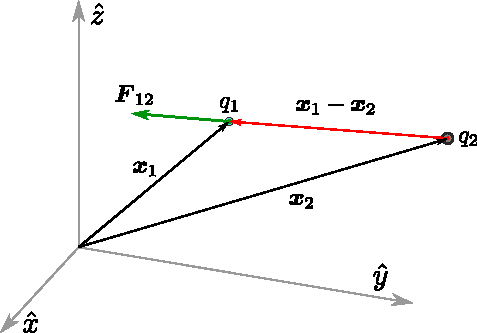
\includegraphics[width=0.5\textwidth]{images/fig_ft1_ejescargas.pdf}	 
	\end{center}
	\caption{Fuerza sobre la carga $q_1$ debida a la carga $q_2$.}
	\label{fig_ft1_ejescargas}
\end{figure} 

Cuando la carga $q_1$ es suficientemente pequeña como para no perturbar a la carga $q_2$ que origina la fuerza, se puede 
utilizar la ley de Coulomb para definir el campo eléctrico según
\[
	\vb{E}_{12}(\vb{x}_1) \equiv \lim_{q_1 \to 0} \frac{\vb{F}_{12}}{q_1}.
\]

Para una distribución discreta de $N$ cargas $q_i$ y tomando $\vb{x}_1 \equiv \vb{x}$ se tiene
\[
	\vb{E}(\vb{x}) = \sum_{i=1}^N \; q_i \frac{(\vb{x} - \vb{x}_i)}{|\vb{x} - \vb{x}_i |^3}.
\]
En el límite en que las cargas están lo suficientemente próximas como para considerar que forman se tiene una distribución
de carga de volumen $\rho(\vb{x})$, la expresión del campo adopta la forma de una integral
\[
	\vb{E}(\vb{x}) = \int_{V'} \rho(\vb{x}') \frac{(\vb{x} - \vb{x}')}{|\vb{x} - \vb{x}' |^3} \: dV' 
\]
donde $V'$ es el volumen de integración. En general \vb{x} es el llamdo punto campo y $\vb{x}'$ punto fuente.

\subsection{Conservación de la carga}

Aceptaremos el principio de conservación de la carga; la carga eléctrica no se genera ni se destruye. 
Considerando una región $\Omega$ en el espacio (cuya frontera está fija) la carga total encerrada en la
misma es 
\[
	Q(t) = \int_\Omega \rho(\vb{x}',t)\: d\Omega,
\]
siendo su variación temporal 
\[
	\dtot{Q(t)}{t} = \int_\Omega \dpar{\rho(\vb{x}',t)}{t} \: d\Omega,
\]
donde la derivada total se transforma en una derivada parcial debido a que el volumen es fijo.
\notamargen{Acá creo que la derivada debería ser la parcial desde el vamos. Check!}

La conservación de la carga nos dice que como la carga no aparece ni desaparece mágicamente, entonces
la variación de la carga contenida en $\Omega$ en cualquier instante de tiempo se debe al flujo neto de 
carga de la misma; es decir a la diferencia entre la que abandona la región y aquella que entra.
Como ilustra esquemáticamente la Figura \ref{conserv_carga}, la variación de carga $\Delta Q$ en un
dado $\Delta t$ corresponde a la diferencia entre las entrantes y las salientes.

La forma que tiene ese flujo se construye a partir del análisis ilustrado en el inserto de la figura.
Allí se ve un elemento pequeño $\delta \Omega$ que linda con la frontera de la región. Este elemento
$\delta V$ es lo suficientemente pequeño como para que en su interior el campo de velocidad de
las cargas sea constante. La {\it caja} $\delta V$ tiene un volumen que se puede expresar $\ell \delta S$
(longitud de la caja por área de la base). La longitud $\ell $ se elige como
$ \ell = v_n \delta t$, donde $v_n$ es la componente de la velocidad normal a la superficie. Así elegido, 
el volumen $\delta V = v_n \delta t \delta S$ representa el volumen que pasaría a través de $\delta S$ 
en el tiempo $\delta t$. En efecto, la partícula más lejana del borde $\delta S$ que está a distancia $\ell$ 
recorrerá en $\delta t$ justamente esa distancia (la velocidad $v$ es constante para todo el elemento).
Si la velocidad estuviese orientada hacia adentro, entonces tendríamos un bloque similar de carga 
entrante, y el razonamiento es el mismo.

La cantidad de carga $\delta Q$ que atraviesa el área $\delta S$ será entonces 
\[
	\delta Q = \rho \delta V = \rho v_n \delta S \delta t = \rho \vb{v} \cdot (\hat{n} \delta S) \delta t
\]
donde se ha expandido la velocidad normal. Entonces la variación de la carga en el elemento es
\[
	\frac{\delta Q}{\delta t} = \rho \vb{v} \cdot (\hat{n} \delta S).
\]

Si el producto escalar entre la velocidad y la normal es positivo entonces esto significa que la carga
abandona la superficie mientras que el caso contrario implica carga entrando en la misma. Entonces 
debemos ajustar la expresión anterior con un signo menos. Entonces, pasando al continuo
\[
	\dpar{Q}{t} = - \int_{\partial\Omega} \: \vb{J} \cdot d\vb{S}
\]
donde $\vb{J} = \rho \vb{v}$ es el vector densidad de corriente y $d\vb{S} = \hat{n}dS$ es el diferencial
de superficie vectorial.

Entonces, juntando las dos expresiones para la carga tenemos 
\[
	\int_\Omega \dpar{\rho(\vb{x}',t)}{t} \: d\Omega = - \int_{\partial\Omega} \: \vb{J} \cdot d\vb{S},
\]
y aplicando el teorema de la divergencia en el miembro derecho
\[
	\int_\Omega \dpar{\rho(\vb{x}',t)}{t} \: d\Omega = - \int_\Omega \: \divem{J} \: d\Omega,
\]
o bien 
\[
	\int_\Omega \left[ \dpar{\rho(\vb{x}',t)}{t} + \divem{J} \right] \: d\Omega = 0,
\]
y como esto vale para cualquier volumen $\Omega$ se sigue que el corchete debe ser nulo, de modo que se tiene
\[
	\dpar{\rho}{t} + \divem{J} = 0,
\]
que es la ecuación de continuidad de la carga.

% Entonces la carga que existe en una región depende de la tasa con la cual entra a la misma y aquella con la que la abandona.
% La carga total sale de una integral 
% \[
% 	Q = \int_{V'}  \rho(\vb{x}') dV'
% \]
% como muestra la imagen
\begin{figure}[htb]
	\begin{center}
	\includegraphics[width=0.25\textwidth]{images/fig_ft1_conserv.pdf}	 
	\end{center}
	\caption{}
	\label{conserv_carga}
\end{figure} 
% y si el volumen es fijo podemos tomar la derivada con respecto al tiempo que pasa el interior como
% derivada parcial,
% \[
% 	\dtot{Q}{t} = \int_{V'} \dpar{\rho}{t} (\vb{x}') dV' = - \int_{S\equiv\partial V'} \vb{J} \cdot d\vb{S}
% \]
% y el miembro extremo derecho  se debe a que si la carga varía es a consecuencia de que se va en
% forma de flujo. 
% Aplicando el teorema de la divergencia en el miembro derecho,
% \[
% 	\int_{V'} \dpar{\rho}{t} (\vb{x}') dV' = - \int_{V'} \nabla \cdot \vb{J} \; dV'
% \]
% lo cual vale para todo volumen y entonces esto significa que
% \[
% 	\dpar{\rho}{t} + \nabla \cdot \vb{J} = 0
% \]
% que es la ecuación de continuidad de la carga. 
\notamargen{Si fuera $\nabla \cdot \vb{J}=0$ esto significa que las líneas
de \vb{J} no tienen principio ni fin.Check!}

Si es $\divem{J}=0$ no se acumula carga; las líneas de $\vb{J}$ no tienen principio ni fin.
Los problemas de corrientes estacionarias cumplen esta condición. Esta condición en la ecuación de continuidad
nos dice que la distribución de carga no varía con el tiempo.

% =================================================================================================
\section{Interacción magnética}
% =================================================================================================

Cuando se da $\nabla \cdot \vb{J}=0$ hablamos de una corriente estacionaria (no hay acumulación de carga en
ninguna parte). Las corrientes estacionarias producen efectos magnéticos dados por la ley de Biot-Savart
\[
	\vb{B}(\vb{x}) = \frac{1}{c} \int_\Gamma \frac{I d\vb{\ell}' \times (\vb{x} - \vb{x}')}{|\vb{x} - \vb{x}'|^3} 
\]
que es válida para un circuito $\Gamma$, que es una curva --lineal-- que se recorre en sentido positivo (CCW).
Si no puede despreciarse el espesor de un circuito, hay que considerar una integral de volumen y la expresión es 
\[
	\vb{B}(\vb{x}) = 
	\frac{1}{c} \int_{V'} \frac{ \vb{J}(\vb{x}') \times (\vb{x} - \vb{x}')}{|\vb{x} - \vb{x}'|^3} \: dV'.
\]
Luego, la fuerza sobre un circuito lineal $\Gamma$ es
\[
	\vb{F} = \frac{1}{c} \int_\Gamma I d \vb{\ell} \times \vb{B},
\]
mientras que para un volumen se tiene
\[
	\vb{F} = \frac{1}{c} \int_V \vb{J} \times \vb{B} \: dV.
\]
La expresión del torque es
\[
	\vb{\Tau} = \frac{1}{c} \int_V \vb{x} \times (\vb{J} \times \vb{B}) \: dV.
\]

La transformación entre estas integrales puede hacerse merced al siguiente razonamiento,
% \begin{align*}
%  	I d\vb{\ell} \times \vb{B} = \vb{J}  \cdot d\vb{S} d\vb{\ell}  \times \vb{B} =
%   	\cos(\theta) dS \vb{J} d\ell \times \vb{B} = \\
% 	\vb{J} \times \vb{B}  \cos(\theta) dS d\ell  = \vb{J} \times \vb{B}  d\vb{S} \cdot d\vb{\ell}  = 
% 	\vb{J} \times \vb{B}  dV 
% \end{align*}
\[
  	I d\vb{\ell} \times \vb{B} = \vb{J}  \cdot d\vb{S} d\vb{\ell}  \times \vb{B} =
  	\cos(\theta) dS \vb{J} d\ell \times \vb{B} = 
\]
\[
	\vb{J} \times \vb{B}  \cos(\theta) dS d\ell  = \vb{J} \times \vb{B}  d\vb{S} \cdot d\vb{\ell}  = 
	\vb{J} \times \vb{B}  dV 
\]

\subsection{Fuerza de un circuito sobre otro}

La fuerza ejercida por el campo magnético de un circuito 2 sobre otro circuito 1 puede calcularse con un poco de 
paciencia como sigue
\[
	F_{12} = \frac{1}{c} \int_{\Gamma_1} I_1 d\vb{\ell}_1 \times \left\{
	\frac{1}{c} \int_{\Gamma_2} \frac{I_2 d\vb{\ell}_2 \times (\vb{x}_1 - \vb{x}_2)}{|\vb{x}_1 - \vb{x}_2|^3} 
	\right\}
\]
\[
	F_{12} = \frac{I_1 I_2}{c^2} \int_{\Gamma_1} \int_{\Gamma_2} d\vb{\ell}_1 \times \left\{
	\frac{d\vb{\ell}_2 \times (\vb{x}_1 - \vb{x}_2)}{|\vb{x}_1 - \vb{x}_2|^3} 
	\right\},
\]
y utilizando una identidad vectorial, 
\[
	F_{12} = \frac{I_1 I_2}{c^2} \int_{\Gamma_1} \int_{\Gamma_2} d\vb{\ell}_2  \left\{
	\frac{d\vb{\ell}_1 \cdot (\vb{x}_1 - \vb{x}_2)}{|\vb{x}_1 - \vb{x}_2|^3} 
	\right\} - \int_{\Gamma_1} \int_{\Gamma_2} \frac{ (\vb{x}_1 - \vb{x}_2)}{|\vb{x}_1 - \vb{x}_2|^3} 
	\left\{ d\vb{\ell}_1 \cdot d\vb{\ell}_2 \right\}
\]
Luego, se puede reescribir el primer término notando que 
\be
	\frac{ (\vb{x}_1 - \vb{x}_2)}{|\vb{x}_1 - \vb{x}_2|^3} = 
	\nabla_{\vb{x}_2} \frac{ 1 }{|\vb{x}_1 - \vb{x}_2|} =
	- \nabla_{\vb{x}_1} \frac{ 1 }{|\vb{x}_1 - \vb{x}_2|} ,
	\label{ident_vec_posicion}
\ee
de manera que la primer integral resulta 
\[
	- \int_{\Gamma_2} d\vb{\ell}_2 \int_{\Gamma_1} d\vb{\ell}_1 \cdot \nabla_{\vb{x}_1} \frac{ 1 }{|\vb{x}_1 - \vb{x}_2|} ,
\]
la cual es nula porque se está integrando un gradiente en una curva cerrada.
% \[
% 	\int_{\Gamma_1} d\vb{\ell}_1 \cdot \nabla_{\vb{x}_1} = 0.
% \]

Entonces, se tiene 
\[
	F_{12} = - \frac{I_1 I_2}{c^2} \int_{\Gamma_1} \int_{\Gamma_2} \frac{ (\vb{x}_1 - \vb{x}_2)}{|\vb{x}_1 - \vb{x}_2|^3} 
	\left( d\vb{\ell}_1 \cdot d\vb{\ell}_2 \right)
\]
que vale lo mismo si intercambiamos $\Gamma_1$ con $\Gamma_2$ en la integración, lo cual implica
que la fuerza sobre un circuito debida a otro es igual a la fuerza sobre este último debida al primero.
Esto quiere decir que vale el principio de acción y reacción en el caso de corrientes estacionarias.
Si las corrientes no son estacionarias no se tendrá, en general, este resultado. Con corrientes no
estacionarias se generará campo electromagnético y habrá emisión de radiación.


% =================================================================================================
\section{Teorema de Helmholtz}
% =================================================================================================

Nos dice que un campo vectorial está completamente determinado por su divergencia y su rotor.
Por ejemplo, para un campo eléctrico se tiene 
\[
	\vb{E} = \int_{V'} \rho \frac{\vb{x} - \vb{x}'}{|\vb{x} - \vb{x}'|^3} dV' = 
		- \int_{V'} \rho \nabla_{\vb{x}} \frac{ 1 }{|\vb{x} - \vb{x}'|} dV' = 
		- \nabla_{\vb{x}} \int_{V'}   \frac{ \rho }{|\vb{x} - \vb{x}'|} dV' = 
\]
donde la integral que ha resultado dentro del gradiente es la integral de Poisson. Entonces,
\[
	\vb{E} = - \nabla_{\vb{x}} \phi (\vb{x}),
\]
de modo que $\vb{E}$ es un gradiente y por ello 
\[
	\nabla  \times \vb{E} = 0.
\]

Esta última condición implica que el campo electrostático $\vb{E}$ es conservativo, cumple 
$\oint_\Gamma \vb{E}\cdot d\vb{\ell} = 0$, o lo que es lo mismo, $\vb{E}$ es irrotacional.
Hemos hecho la construcción de un potencial electrostático.

\notamargen{
Para el curso de indicial:
\[
	[\pv{A}{B}]_i = \epsilon_{ijk}A_jB_k
\]
\[
	[\rotorm{A}]_i = \epsilon_{ijk}\partial_jA_k
\]
\[
	\epsilon_{ijk}\epsilon_{\ell mn} = \delta_{i\ell}
	\delta_{jm} - \delta_{im}\delta_{j\ell}
\]}

% =================================================================================================
\section{Ley de Gauss}
% =================================================================================================

La idea es considerar el campo ejercido por una carga puntual $q$ en un punto de una superficie $S\equiv\partial\Omega$,
como se ilustra en la Figura \ref{fig_ft1_gauss}.

\begin{figure}[htb]
	\begin{center}
	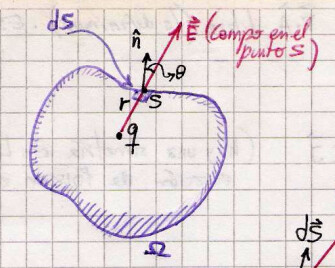
\includegraphics[width=0.35\textwidth]{images/fig_ft1_gauss.jpg}	 
	\end{center}
	\caption{}
	\label{fig_ft1_gauss}
\end{figure} 

El campo en el punto verifica
\[
	\vb{E} \cdot \hat{n} = q \frac{\cos(\theta)}{r^2}
\]
y teniendo en cuenta el diferencial de superifice $dS$
\[
	\vb{E} \cdot \hat{n} dS = q \frac{\cos(\theta)}{r^2} dS
\]
donde el factor $ \cos\theta dS / r^2 $ es el ángulo sólido subtendido por $dS$ desde el punto donde se halla $q$

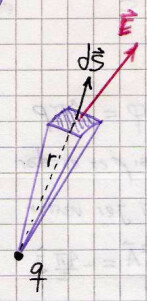
\includegraphics[width=0.15\textwidth]{images/fig_ft1_gauss_solid_angle.jpg}

Podemos escribir 
\[
	\vb{E} \cdot \hat{n} dS = q d\Omega
\]
donde $ d\Omega $ es el diferencial de ángulo sólido. Integrando para todo el volumen
\[
	\int_{S\equiv\partial V} \vb{E} \cdot \hat{n} \; dS = q \int_S d\Omega =
	\begin{cases}
	 0 \quad \textrm{carga exterior}\\
	 4\pi \quad \textrm{carga interior}
	\end{cases}
\]
y la integral es nula si la carga es exterior a $S$ o $4\pi$ si es interior.
En el caso de una cantidad de cargas internas se tendrá, evidentemente,
\[
	\int_S \vb{E} \cdot \hat{n} \; dS = 4\pi \sum_i q_i.
\]

Este hecho se conoce como La ley de Gauss y se expresa 
\[
	\int_S \vb{E} \cdot \hat{n} \; dS = 4\pi Q_n,
\]
donde $Q_n$ es la carga neta dentro de la superficie $S$. Al continuo pasa como 
\[
	\int_S \vb{E} \cdot \hat{n} \; dS = 4\pi \int_V \rho \: dV,
\]
de manera que usando el teorema de la divergencia se obtiene 
\[
	\int_V \divem{E} \; dV = \int_V 4\pi \rho \: dV,
\]
o bien
\[
	\divem{E} = 4\pi \rho.
\]

Lo que es vital en todo este razonamiento es el hecho de que el campo decaiga como $1/r^2$.
Luego, alguna `ley de Gauss' podrá aplicarse a cualquier campo con ese tipo de decaimiento.

Por otro lado si \vb{E} es el gradiente de un potencial $\phi$ la divergencia del campo
\[
	\divem{E} = \Nabla\cdot{(-\Nabla\phi)} = - \lapm\phi = 4\pi \rho
\]
conduce a la ecuación de Poisson para el potencial electrostático,
\[
	\lapm\phi = -4\pi \rho,
\]
cuyo caso particular en el caso $\rho=0$
\[
	\lapm\phi = 0,
\]
constituye la ecuación de Laplace.

Matemáticamente esto significa que la solución de la ecuación no homogénea (Poisson) es suma de 
una solución del homogéneo (Laplace) más una solución particular. 
La carga en el volumen está relacionada con la solución particular.

Por supuesto para resolver cualquiera de estas ecuaciones hace falta dar las correspondientes
condiciones de contorno. Usualmente serán de dos tipos: Dirichlet (valor del potencial en la
superifice) o Newmann (valor de la derivada normal del potencial sobre la superficie).

\subsection{Gauges}

Dado que $\divem{B}=0$ entonces existe un \vb{A} tal que 
\[
	\rotorm{A} = \vb{B}
\]
pero para caracterizar totalmente el \vb{A} tengo la libertad de definir a conveniencia
\[
	\divem{A} \equiv \; \textrm{``el gauge''}.
\]
Casos particulares importantes son el gauge de Coulomb,
\[
	\divem{A} = 0
\]
de manera que como 
\[
	\Nabla \times (\rotorm{A}) = \Nabla(\divem{A}) - \lapm{\vb{A}} = \frac{4\pi}{c}\vb{J}
\]
se llega para el potencial electromagnético, bajo el gauge de Coulomb, a que 
\[
	\lapm{\vb{A}} = - \frac{4\pi}{c}\vb{J} 
\]

	\begin{table}[ht]
	\centering
        \begin{tabular}{|c|c|}
		\hline
		Electrostática & Magnetostática \\
		\hline 
		 & \\
		$\displaystyle \vb{F}_{12} = \frac{q_1 q_2 ( \vb{x}_1 - \vb{x}_2 )}{ |\vb{x}_1 - \vb{x}_2|^3 } $
		& 
		$ \displaystyle d\vb{F}_{12} = \frac{1}{c^2} \frac{ I_1 d\vb{\ell}_1 \times J_2 d\vb{\ell}_2 \times ( \vb{x}_2 - \vb{x}_1 )}
		{ |\vb{x}_2 - \vb{x}_1|^3 }$
		\\
		 & \\
		\hline
		& \\
		$\displaystyle{\vb{E} = \int_{V'} \frac{\rho(\vb{x}')(\vb{x}-\vb{x}')}{|\vb{x}-\vb{x}'|^3} dV' 
		}$ & $\displaystyle{\vb{B} = \frac{1}{c} \int_{V'} \frac{\vb{J}(\vb{x}') \times 
		(\vb{x}-\vb{x}')}{|\vb{x}-\vb{x}'|^3} dV'}$ \\
		& \\
		\hline
		Ley de Gauss & Ley de Ampere \\
		& \\
		$\displaystyle{\int_S \vb{E}\cdot d\vb{S} = 4\pi Q_n}$ &
		$\displaystyle{\int_\Gamma \vb{B}\cdot d\vb{\ell} = \frac{4\pi}{c} I_c}$ \\
		& \\
		\hline
		Ecuaciones electrostáticas & Ecuaciones magnetostáticas \\
		&\\
		$\divem{E} = 4\pi\rho$ & $\divem{B} = 0$ \\
		&\\
		$\rotorm{E} = 0$ & $\rotorm{B} = \frac{4\pi}{c}\vb{J}$ \\
		& \\
		\hline
		& \\
		$\vb{E} = - \Nabla\phi$ & $\vb{B} = \rotorm{A}$ \\
		& \\
		\hline
		\end{tabular} 
		\caption{Recetario de ecuaciones básicas para la electrostática y la
		magnetostática.}
	\end{table} 

\notamargen{Estos comentarios sobre vectores irán en el apéndice matemático vectorial.}
La operación de tomar rotor y el producto vectorial cambian el carácter de los vectores: de
polares pasan a axiales y viceversa.

El laplaciano es la divergencia del gradiente, dos operaciones que no cambian el carácter de
un vector. Luego, el laplaciano preserva la simetría.

La fuerza general sobre una distribución de carga es
\[
	\vb{F} = \int_{V'} \rho \vb{E} \: dV' + \frac{1}{c} \int_{V'} \vb{J} \times \vb{B} \: dV'. 
\]

\notamargen{
A partir de la tabla hay mucho para mencionar. Por ejemplo, el hecho de la separación total
de fenómenos, que la fuerza magnética es una diferencial (no hay cargas puntuales magnéticas),
que el potencial en un caso es escalar mientras que en el otro es vectorial, etc.
}

\subsection{Delta de Dirac}

Una densidad de carga puntual se puede escribir mediante una delta de Dirac de acuerdo a
\[
	\rho(\vb{x}') = q\: \delta (\vb{x} - \vb{x}') = \begin{cases}
	                                               0 \qquad \vb{x} \neq \vb{x}' \\
	                                               \infty \qquad \vb{x} = \vb{x}'\\
	                                              \end{cases}
\]
siendo las dimensiones de la delta las de $1/L^3$ y cumpliéndose 
\[
	\int_{V'} \delta (\vb{x} - \vb{x}') dV' = 1.
\]

La delta de Dirac se puede aproximar con ciertas funciones matemáticas con gráficas como el 
siguiente 

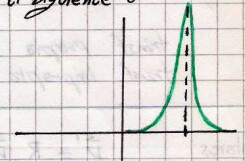
\includegraphics[width=0.25\textwidth]{images/fig_ft1_delta_dirac.jpg}

La delta de Dirac cumple las siguientes propiedades
\[
	\int f(\vb{x}) \delta(\vb{x} - \vb{x}_0) dx = f(\vb{x}_0)
\]
\[
	\int f(\vb{x}) \delta' (\vb{x} - \vb{x}_0) dx = -f'(\vb{x}_0)
\]
\[
	\int f(\vb{x}) \delta^n (\vb{x} - \vb{x}_0) dx = (-1)^n f^n(\vb{x}_0)
\]
\[
	\delta[f(x)] = \frac{\delta(\vb{x}-\vb{x}_0)}{|f'(\vb{x}_0)|} \qquad \qquad f(\vb{x}_0) = 0
\]

En coordenadas cartesianas es
\[
	\delta(\vb{x}-\vb{x}_0) = \delta(x-x_0)(y-u_0)(z-z_0)
\]
y para curvilíneas, como el elemento diferencial y el de volumen son  
\[
	d\vb{x} = h_1 dq_1 \hat{e}_1 + h_2 dq_2 \hat{e}_2 + h_3 dq_3 \hat{e}_3 
	\qquad 	dV = h_1 h_2 h_3 dq_1 dq_2 dq_3
\]
se tiene
\[
	\delta (\vb{x} - \vb{x}') = \frac{1}{h_1h_2h_3} \delta(q_1-q_1') \delta(q_2-q_2') \delta(q_3-q_3')
\]
donde $q_1, q_2$ y $q_3$ son coordenadas curvilíneas generales y $h_1h_2h_3$ es el jacobiano
de la transformación.
Puntualmente para coordenadas esféricas se tiene 
\[
	\delta (\vb{x} - \vb{x}') = \frac{1}{r^2 \sin\theta} 
	\delta(r-r') \delta(\theta-\theta') \delta(\varphi-\varphi')
\]
donde no está definido para $\theta=0$. Si $r_0=0$ entonces se tiene 
\[
	\delta(\vb{x}) = \frac{\delta(r)}{4\pi r^2}
\]
que involucra un factor de normalización.

Para un casquete esférico se tendrá $\rho(\vb{x}) = \sigma \delta(r-R) $ y para una corriente
circulando por un plano como ilustra la figura

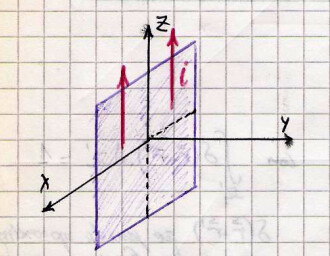
\includegraphics[width=0.25\textwidth]{images/fig_ft1_deltas_ejemplos.jpg}
se tiene $\vb{J} = g \delta(y) \hat{z}$. Estas deltas, al ser unidimensionales tienen unidades
de $1/L^{-1}$ de manera que las otras unidades serán llevadas por $\sigma$ y $g$.

\subsection{Vectores polares y axiales ante transformaciones}

Las transformaciones propias son aquellas con determinante 1 y las impropias las que tienen determinante
distinto de 1.
Entonces, para un vector polar $\vb{p}$ y siendo $R$ la matriz de la transformación y $|R|$ su determinante, 
se tiene 
\[
	\vb{p}' = R \: \vb{p},
\]
mientras que para un vector axial \vb{a}
\[
	\vb{a}' = |R| R \: \vb{a}.
\]

Aquí se ve que ante una transformación propia ambos vectores transforman igual pero ante una impropia 
hay un cambio asociado al determinante.

Un vector polar sufre reflexión especular mientras que un vector axial ({\it pseudovector})
sufre una antireflexión especular. Ver la figura.

\begin{figure}[htb]
	\begin{center}
	\includegraphics[width=0.6\textwidth]{images/fig_ft1_reflexvect.pdf}	 
	\end{center}
	\caption{A la izquierda está el comportamiento polar mientras que a la derecha
	se halla el comportamiento axial.}
\end{figure} 

Para un campo escalar, como podría ser la temperatura $T(\vb{x})$ una rotación deja invariante el valor
del campo 

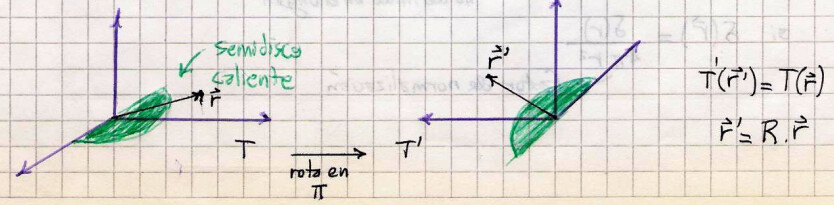
\includegraphics[width=0.8\textwidth]{images/fig_ft1_rotacion_escalar.jpg}

En el caso de un campo vectorial 

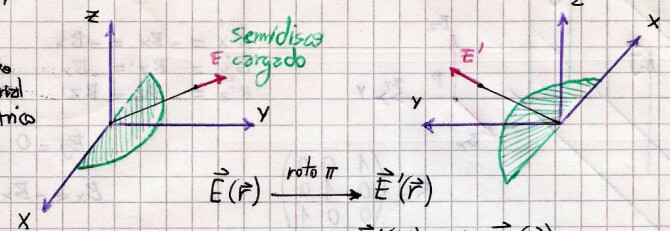
\includegraphics[width=0.8\textwidth]{images/fig_ft1_rotacion_vectorial.jpg}\\
se ve que 
\[
	\vb{E}'(\vb{x}') = R\vb{E}( R\vb{x}).
\]

En el caso de una simetría por reflexión como la de la figura 

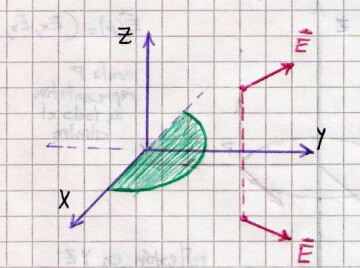
\includegraphics[width=0.4\textwidth]{images/fig_ft1_reflexion_vectorial.jpg}\\
el campo en una situación simétrica cumplirá 
\[
	\vb{V}(\vb{x}') = R \vb{V}(\vb{x})
\]
mientras que un campo escalar sería $T(\vb{x}')=T(\vb{x})$.

% Ejemplo eléctrico

\begin{ejemplo}{\bf Ejemplo de problema simétrico (eléctrico)}

Consideremos un plano infinito cargado con una densidad de carga $\sigma$, según se
ve en la figura bajo estas líneas. 
La idea es que el campo en un punto $P$ será 
\[
	\vb{E}(P) = (E_x, E_y, E_z), 
\]
es decir que en principio tendrá los tres componentes.

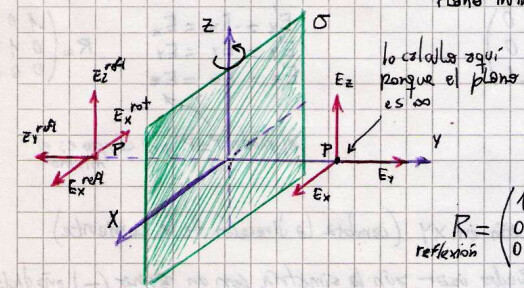
\includegraphics[width=0.4\textwidth]{images/fig_ft1_ej_plano_cargado.jpg}

Del otro lado del plano la situación es la misma de manera que se tiene una simetría de 
reflexión en $xz$. La matriz de una reflexión es 
\[
	R = \begin{pmatrix}
		1 & 0 & 0 \\
		0 & -1 & 0 \\
		0 & 0 & 1
	\end{pmatrix}
\]
y entonces se tienen las relaciones (compruébese en la figura)
\be
	E_x' = E_x, \qquad E_y' = -E_y, \qquad E_z' = E_z.
	\label{simetria_refl}
\ee

Luego, otra simetría es sencillamente rotar el plano un ángulo $\pi$ en torno a $\hat{z}$,
y esta rotación será \notamargen{poner matriz de rotación en apéndice}
\[
	R = \begin{pmatrix}
		-1 & 0 & 0 \\
		0 & -1 & 0 \\
		0 & 0 & 1
	\end{pmatrix}
\]
que implica 
\be
	E_x' = -E_x, \qquad E_y' = -E_y, \qquad E_z' = E_z.
	\label{simetria_rot}
\ee

Como ambas simetrías conllevan a la misma situación física, deben ser ciertas las relaciones 
\eqref{simetria_refl} y \eqref{simetria_rot} de modo que como $E_x = - E_x$ se debe cumplir 
que $E_x = 0$.

Se puede hacer el mismo razonamiento para la simetría de reflexión en torno a $xy$ puesto que
dicho plano separa dos semiespacios especularmente idénticos. En este caso como $P$ se halla
sobre dicho plano basta una rotación en un ángulo de $2\pi$, que deja el campo en el mismo
sitio para obtener la relación $E_z = - E_z$ lo cual implica que $\vb{E} = E_y \hat{y}$.
\end{ejemplo}

% Ejemplo magnético 

\begin{ejemplo}{\bf Ejemplo de problema simétrico (magnético)}

Consideremos un plano infinito por el cual circula una corriente cuya densidad de corriente \vb{J}
está mostrada en la figura bajo estas líneas. 
La idea es que el campo magnético \vb{B} en un punto $P$ será 
\[
	\vb{B}(P) = (B_x, B_y, B_z), 
\]
es decir que en principio tendrá los tres componentes.
 
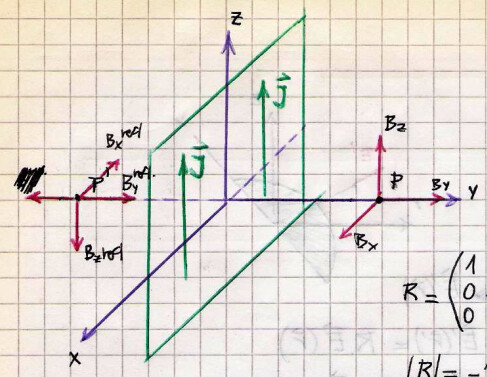
\includegraphics[width=0.4\textwidth]{images/fig_ft1_ej_plano_corriente.jpg}

Dado que este campo es un pseudovector, debe reflejarse {\it mal} en el plano, como se ilustra en
la figura. La reflexión en el plano $xz$ lleva a 
\be
	B_x' = -B_x, \qquad B_y' = B_y, \qquad B_z' = -B_z,
	\label{Bsimetria_refl}
\ee
que proviene de la matriz de reflexión $R$ del caso anterior (es la misma porque giramos en el
mismo sentido el mismo plano) a la cual se le ha multiplicado el determinante $|R|=-1$ de la misma
puesto que el campo \vb{B} es un pseudovector.

La rotación en torno a un ángulo $\pi$ del plano es también una simetría, representada por la misma
matriz de rotación $R$ del ejemplo anterior por lo cual se tendrán 
\be
	B_x' = -B_x, \qquad B_y' = -B_y, \qquad B_z' = B_z,
	\label{Bsimetria_rot}
\ee 
de lo cual se deduce que $ B_y = B_z = 0 $. El campo magnético sólo puede tener componente en $\hat{x}$,
es decir que se escribirá como $\vb{B} = B_x \hat{x}$.
Este hecho también puede deducirse cualitativamente utilizando la regla de la mano derecha.
\end{ejemplo}


\begin{ejemplo}{\bf Hilo cargado e hilo con corriente}

Consideraremos ahora dos situaciones geométricas idénticas (un hilo infinito) pero en primer lugar el
caso en que está cargado uniformemente y en segundo lugar el caso en que por el mismo circula una
corriente estacionaria $i$. 

En el caso del hilo cargado se quiere determinar las simetrías del campo $\vb{E}$ en un punto $\vb{P}$,

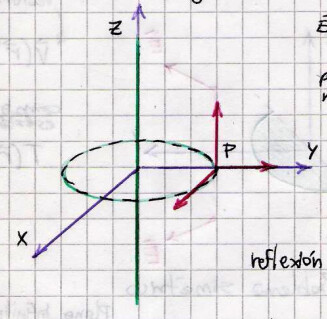
\includegraphics[width=0.4\textwidth]{images/fig_ft1_ej_hiloE.jpg}

El punto \vb{P} es representativo de todo el cilindro. La simetría de reflexión en $xy$ no hace que el
punto cambie ($\vb{P}' = \vb{P}$) pero el campo debe reflejarse, de lo cual se tiene 
\[
	E_x' = E_x, \qquad E_y' = E_y, \qquad E_z' = -E_z.
\]
Luego, la rotación en ángulo $2\pi$ implica que $E_z = -E_z$ y por ende el componente $z$ debe ser nulo.

Por otra parte, la simetría de reflexión en $yz$ de igual manera lleva a $E_x = -E_x$ de forma que
el campo \vb{E} de un hilo cargado solo tendrá componentes en $\hat{y}$.

En el caso del hilo con una corriente que circula por el mismo se debe notar que ahora la corriente tiene
dirección con lo cual la simetría de reflexión en $xy$ se verifica si incorporamos un signo menos que dé
cuenta del cambio en la dirección de la corriente

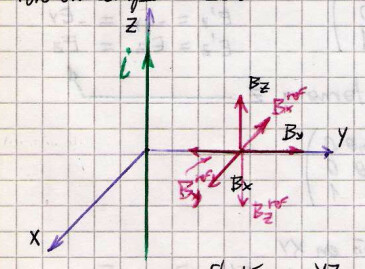
\includegraphics[width=0.4\textwidth]{images/fig_ft1_ej_hiloB.jpg}

Entonces por una parte tenemos la reflexión que, luego del añadido del signo extra, da las igualdades 
\[
	B_x' = B_x, \qquad B_y' = B_y, \qquad B_z' = -B_z,
\]
que al combinarse con las que resultan de que los puntos son el mismo $\vb{P}=\vb{P}'$ (o digamos que 
giramos en ángulo $2\pi$) resultan en que $B_z = -B_z$ y por ende $B_z$ es nulo.

La reflexión en $yz$ no requiere el signo menos extra por el cambio de la corriente, así que da sencillamente 
\[
	B_x' = B_x, \qquad B_y' = -B_y, \qquad B_z' = -B_z,
\]
y luego la igualdad de puntos establece 
\[
	B_x' = B_x, \qquad B_y' = B_y, \qquad B_z' = B_z,
\]
de modo que, igualando ambas expresiones, tiene que ser $ B_y = B_z = 0 $. Entonces el campo $\vb{B}$ sólo
tiene componentes en $\hat{x}$, es un campo anular.
\end{ejemplo}

\notamargen{En estos ejemplos creo que es más beneficiosa la notación de la carpeta, ecuaciones `triples'.}


Como se vió en el ejemplo anterior, una reflexión más una rotación permite eliminar componentes 
de campo.


Una simetría más una rotación-traslación permite eliminar dependencias.

Lo primero que debe hacerse es escribir bien la \vb{J} a partir del dato de la corriente
(que es el que se suele tener) mediante
\[
	i = \int_S \vb{J} \cdot d \vb{S}
\]
En cambio, para \vb{A} es más fácil usar
\[
	\vb{B} = \rotorm{A}
\]
y despejar de aquí la ecuación diferencial que emplear
\[
	\vb{A} = \frac{1}{c} \int_V \frac{\vb{J}}{|\vb{x}-\vb{x}'|} dV
\]


\section{El potencial vector}

Por la ley de Biot y Savart, el campo \vb{B} debido a una densidad 
de corriente en un volumen puede obtenerse a partir de
\be
	\vb{B} = 
	\frac{1}{c} \int_{V'} \frac{\vb{J}(\vb{x}') \times (\vb{x}-\vb{x}')}{|\vb{x}-\vb{x}'|^3} dV' .
	\label{campo_B}
\ee

Utilizando la identidad de \eqref{ident_vec_posicion}, con el gradiente respecto del punto campo,
y la identidad vectorial
\[
	\Nabla \times (\phi \vb{F} ) = \phi \rotorm{F} - \vb{F} \times \Nabla \phi
\]
la expresión \eqref{campo_B} para el campo magnético resulta en 
\[
	\vb{B} = \Nabla_x \times \frac{1}{c} \int_{V'} \frac{\vb{J}(\vb{x}')}{|\vb{x}-\vb{x}'|} dV'
\]
de modo que
\be
	\vb{A} = \frac{1}{c} \int_{V'} \frac{\vb{J}(\vb{x}')}{|\vb{x}-\vb{x}'|} dV'
	\label{potvec}
\ee
pero como el potencial vector se define a menos del gradiente de un escalar, resulta
\[
	\vb{A}' \equiv \vb{A} + \Nabla \psi
\]
es tan buen potencial vector como \vb{A} puesto que los rotores verifican $\rotorm{A}=\rotorm{A}'=\vb{B}$,
de lo cual extraemos en conclusión que el potencial vector está definido a menos del gradiente de una
función escalar.
\notamargen{Reacomodar estas cosas.}

Cada componente de \vb{A} en el caso de que $\Nabla\psi=0$ puede verse como una integral de Poisson.

Ahora bien, si se toma el rotor del campo \vb{B}, lo cual es tomar el rotor de \vb{A}, se tiene
\[
	\rotorm{B} = \Nabla\times\left( \frac{1}{c} \int_{V'} \frac{\vb{J}(\vb{x}')}{|\vb{x}-\vb{x}'|} dV' \right)
\]
y usando la identidad del rotor de un rotor (ver apéndices XXX) resulta descompuesto en dos términos de
acuerdo a
\[
	\rotorm{B} = 
	\Nabla\left( \Nabla \cdot \left[ \frac{1}{c} 
		\int_{V'} \frac{\vb{J}(\vb{x}')}{|\vb{x}-\vb{x}'|} dV' \right] \right) -
	\nabla^2 \left( \frac{1}{c} \int_{V'} \frac{\vb{J}(\vb{x}')}{|\vb{x}-\vb{x}'|} dV' \right),
\]
el gradiente de una divergencia y el laplaciano de un vector. Trabajaremos cada uno de ellos por 
separado. 

Dado que la divergencia es con respecto a las coordenadas de \vb{x} y la integración es con respecto
a las coordenadas \vb{x}' puede introducirse la misma bajo el signo integral y entonces
\[
	I_1 = \frac{1}{c} 
		\int_{V'} \vb{J}(\vb{x}') \Nabla \cdot \left[ \frac{ 1 }{|\vb{x}-\vb{x}'|} \right] dV'
		= - \frac{1}{c} 
		\int_{V'} \vb{J}(\vb{x}') \Nabla' \cdot \left[ \frac{ 1 }{|\vb{x}-\vb{x}'|} \right] dV'
\]
donde la última igualdad se debe al cambio de las coordenadas contra las cuales se deriva.
Ahora notando la siguiente expresión para la divergencia del integrando en el potencial vector,
\[
	\Nabla' \cdot \left[ \frac{ \vb{J}(\vb{x}') }{|\vb{x}-\vb{x}'|} \right] =
	\frac{ \Nabla' \cdot \vb{J}(\vb{x}') }{|\vb{x}-\vb{x}'|} +
	 \vb{J}(\vb{x}') \cdot \Nabla' \left[ \frac{ 1 }{|\vb{x}-\vb{x}'|} \right]
\]

Considerando que $\Nabla'\cdot\vb{J}(\vb{x}')=0$, lo cual se verifica si
la corriente es estacionaria se tiene 
\[
	I_1 = - \frac{1}{c} 
	\int_{V'} \Nabla' \cdot \left[ \frac{ \vb{J}(\vb{x}')  }{|\vb{x}-\vb{x}'|} \right] dV'
\]
expresión a la cual se puede aplicar el teorema de la divergencia en una superficie 
$ S' = \partial V' $ que englobe completamente a la distribución de corrientes dada por 
$\vb{J}$ (y esto siempre se puede hacer si \vb{J} está acotada) resultando en 
\[
	I_1 = \frac{1}{c} \int_{S'} 
	\frac{ \vb{J}(\vb{x}')  }{|\vb{x}-\vb{x}'|} \cdot \hat{n} dS' = 0.
\]

El segundo término es 
\[
	I_2 = \nabla^2 \left( \frac{1}{c} \int_{V'} \frac{\vb{J}(\vb{x}')}{|\vb{x}-\vb{x}'|} dV' \right)
\]
donde el laplaciano, por la misma razón, también puede ser llevado dentro de la integral lo 
cual resulta en 
\[
	I_2 = \frac{1}{c} \int_{V'} \vb{J}(\vb{x}') \: \nabla^2 \left( \frac{1}{|\vb{x}-\vb{x}'|} \right) dV'
	= \frac{4 \pi }{c} \int_{V'} \vb{J}(\vb{x}') \: \delta( \vb{x}-\vb{x}') dV',
\]
luego de utilizar el valor del laplaciano de la diferencia entre puntos campo y fuente. La
integral es nula salvo en el caso en el cual el punto \vb{x} se halle dentro de $V'$, lo cual 
suponemos que es cierto obteniéndose entonces 
\[
	I_2 = - \frac {4 \pi} {c} \vb{J}(\vb{x}).
\]

Juntando todos los resultados de estas excursiones, arribamos a 
\[
	\rotorm{B} = \frac{4 \pi} {c} \vb{J}(\vb{x}).
\]

Integrando esta ecuación de Maxwell sobre una superficie $S$ cuya frontera es una curva
cerrada $\Gamma$ se tiene 
\[
	\int_S \rotorm{B} \cdot d\vb{S} = \frac{4\pi}{c} \int_S \vb{J}(\vb{x}) \cdot d\vb{S}
\]
y por el teorema de Stokes arribamos a
\[
	\int_{\Gamma\equiv\partial S} \vb{B}\cdot d\vb{\ell} = \frac{4\pi}{c} I_\Gamma
\]
que es la ley de Ampere. Notemos que $I_\Gamma$ es la corriente concatenada por el lazo $\Gamma$.

Además, volviendo a la identidad vectorial del doble rotor, 
\[
	\rotorm{B} = \Nabla\times(\rotorm{A}) = \Nabla(\divem{A}) - \nabla^2 \vb{A} = \frac{4\pi}{c}\vb{J}
\]
que se simplifica utilizando el gauge de Coulomb, $\divem{A}=0$, para llegar a 
\[
	\nabla^2 \vb{A} = -\frac{4\pi}{c}\vb{J},
\]
que es una ecuación de Poisson vectorial para la magnetostática.

Magnetostática y electrostáctica son gobernadas por ecuaciones de Poisson para potenciales $\vb{A},\phi$ y
el problema entonces se reduce a resolverlas para luego hallar los campos por derivación.

\begin{ejemplo}{\bf Ejemplo de Gauss law y Ampere law}

Se tiene un hilo cargado con una densidad lineal de carga $ \lambda $, tomando una superficie gaussiana
cilindrica coaxial y concéntrica con el mismo 

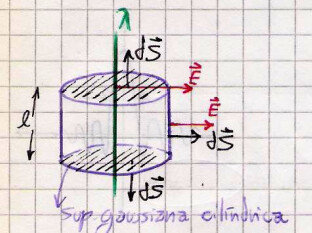
\includegraphics[width=0.4\textwidth]{images/fig_ft1_gausslaw.jpg}

se tiene 
\[
	\int \vb{E}\cdot d\vb{S} = 4 \pi Q,
\]
y dada la forma del campo en cada superficie se tiene
\[
	E 2 \pi r \ell = 4 \pi \lambda \ell
\]
de modo que 
\[
	E = \frac{2 \lambda}{r}.
\]

En el caso de un toro por el cual circula una corriente $i$ en cada vuelta de la espira se definen dos
circuitos $\Gamma_1$ y $\Gamma_2$ según al figura debajo

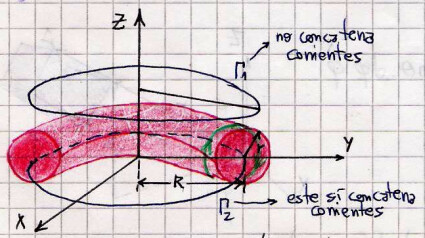
\includegraphics[width=0.4\textwidth]{images/fig_ft1_amperelaw.jpg}

El campo $\vb{B}$ estará en $\phiver$ y además no depende de $\vp$ por la simetría (en coordenadas
cilíndricas), entonces para un dado $r_0$ y $z_0$ será una constante en $\phiver$.
Entonces
\[
	\int_\Gamma \vb{B}\cdot d\vb{\ell} = \frac{4 \pi }{c} I_c
\]
y para los circuitos de la figura 
\[
	\int_{\Gamma_1} \vb{B}\cdot d\vb{\ell} = 0 \qquad \vb{B} = 0
\]
de modo que el campo magnético será nulo fuera. En cambio, dentro
\[
	\int_{\Gamma_1} \vb{B}\cdot d\vb{\ell} = \frac{4\pi}{c}Ni \qquad B = \frac{2Ni}{Rc}
\]

\notamargen{Estaría bueno hacer un análisis fino de las aproximaciones, hacer el cálculo
posta de los campos magnéticos y ver que las consideraciones de simetría funcionan.
Este ejemplo, pese a lo boludo, es muy ilustrativo.}

\end{ejemplo}


\section{Resolviendo problemas de potencial}

Estaremos interesados en resolver las ecuaciones de Poisson y de Laplace en un cierto recinto.
Para tener soluciones únicas necesitaremos condiciones de contorno de tipo Dirichlet o de tipo Newmann (derivada
normal en el contorno).


\subsection{Unicidad de problemas de potencial}

La unicidad de la solución permite la fabricación de problemas equivalentes para otras soluciones.
Si dos problemas satisfacen iguales condiciones de contorno entonces en el recinto encerrado por
ese contorno tienen igual solución.

Si en un recinto $R$
\be
	\phi_1|_{cont} = \phi_2|_{cont}
	\label{potnounico}
\ee
pero se da para el interior de $R$ que $\phi_1\neq\phi_2$ entonces se tiene sucesivamente
\[
	U \equiv \phi_1 - \phi_2 \qquad \qquad \Nabla U = \Nabla \phi_1 - \Nabla \phi_2
\]
\[
	\lapm{U} = \lapm{\phi_1} - \lapm{\phi_2} = -4\pi \rho + 4\pi\rho = 0
\]
\[
	\Nabla\cdot\left( U\Nabla U \right) = U\left( \Nabla\cdot\Nabla U \right) + \Nabla U \cdot \Nabla U
\]
\[
	\int_V \Nabla\cdot\left( U\Nabla U \right) dV = 
	\int_V U \lapm{U}  + (\lapm{U})^2 dV =  \int_V (\lapm{U})^2 dV
\]
llegando al último miembro porque el potencial $U$ cumple la ecuación de Laplace. Luego,
\[
	\int_V (\lapm{U})^2 dV = \int_S U\Nabla{U} \cdot d\vb{S} = 0
\]
habiéndose pasado a la integral de superficie por el teorema de la divergencia y anulando 
el valor global porque 
$U$ en el contorno es nula (recuérdese \eqref{potnounico}). Además, 
\[
	\Nabla{U} \cdot d\vb{S}  \longrightarrow \left.\dpar{U}{\hat{n}}\right|_{cont}
\]
luego,
\[
	\Nabla U = 0 \qquad \Nabla\phi_1 = \Nabla\phi_2 
\]
y entonces
\[
	\phi_1 = \phi_2 .
\]
a menos, por supuesto, de una constante.

\notamargen{Veo la idea acá pero esto hay que hacerlo con mucho cuidado.
Tal vez garabatear en papel y pasar los pasos importantes aquí.
Utilizar claramente las condiciones de contorno; Dirichlet o Newmann.}


Los problemas que siguen parecen ser correspondientes a cálculo de campos a lo F3, de manera que
tendrán que reubicarse luego. Suponemos que son guía 1.
\begin{ejemplo}{\bf Problema 6}

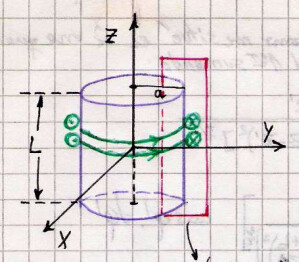
\includegraphics[width=0.3\textwidth]{images/fig_ft1_setproblemasG1_1.jpg}

La integral del campo magnético es
\[
	\vb{B}(\vb{x}) = \frac{1}{c}\int_\Omega  
	\frac{ \vb{J}(\vb{x}) \times (\vb{x}-\vb{x}')}{|\vb{x}-\vb{x}'|^3} d\Omega
\]
pero primeramente se busca obtener la corriente, cuya distribución es proporcional a la delta
de Dirac con alguna constante de proporcionalidad que hay que hallar. Entonces
\[
	I_T = \int_S \vb{J}\cdot d\vb{S} = \int_0^\infty \int_{-L/2}^{L/2} \alpha \delta(y-a) dy dz =
	\alpha \int_{-L/2}^{L/2} dz = \alpha L = I n L
\]
de lo cual se obtiene $\alpha = n L$ y donde se ha usado $n=N/L$.

Luego,
\[
	\vb{B}(\vb{x}) = \frac{1}{c} \int_{-L/2}^{L/2} \int_0^{2\pi} \int_0^a 
	\frac{ n I \delta(r'-a) r' \phiver \times ( -r'\cos\vp'\xver - r'\sin\vp'\yver + (z-z')\zver) }
	{({r'}^2 + [z-z']^2)^{3/2}} \: dr' d\vp' dz'
\]
y colapsando la delta en $r$,
\[
	\vb{B}(\vb{x}) = \frac{n I}{c} \int_{-L/2}^{L/2} \int_0^{2\pi} 
	\frac{ a' \phiver \times ( -a'\cos\vp'\xver - a'\sin\vp'\yver + (z-z')\zver) }
	{({a'}^2 + [z-z']^2)^{3/2}} \: d\vp' dz'
\]
donde el producto vectorial requiere previamente convertir $\phiver$ a cartesianas.
Entonces, usando la regla mnemotécnica sabida,
\[
	\begin{vmatrix}
	\xver & \yver & \zver \\
	 -\sin\vp' & -\cos\vp' & 0 \\
	 -a\cos\vp' & -a\sin\vp' & (z-z')\\
	\end{vmatrix}
	= \cos\vp'(z-z')\xver + \sin\vp'(z-z')\yver + a\zver
\]

Las integrales en $\cos\vp'$ y $\sin\vp'$ dan cero porque son trigonométricas entre 0 y 2$\pi$.
Luego
\[
	\vb{B}(0,0,z) = \frac{n I 2 \pi a^2}{ c } \int_{-L2}^{L/2} \frac{ dz'}{( a^2 + [z-z']^2)^{3/2}} \: \zver =
	\frac{2 \pi n I}{c } \left( \frac{L/2 + z}{a^2 + (z+L/2)^2 } + \frac{L/2 - z}{a^2 + (L/2 - z)^2} \right)
\]
\notamargen{Acá parece que se simplificaba el $a^2$.}
y se obtiene 
\[
	\vb{B}(0,0,z) = \frac{2 \pi n I}{c}\left( \cos\theta_2 + \cos\theta_1 \right)
\]

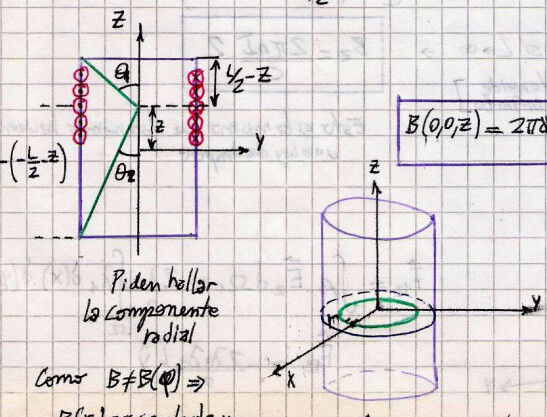
\includegraphics[width=0.4\textwidth]{images/fig_ft1_setproblemasG1_2.jpg}

Piden hallar la componente radial. Como $B$ no depende de $\vp, B(r_0)$ es constante y entonces situándose
en $\xver$ sabré que es válido en un círculo $r$
\[
	\vb{B}(\vb{x}) =  \frac{nIa}{c}\int_{-L2}^{L/2} \int_0^{2\pi} 
	\frac{\hat{\vp}\times (\vb{x}-\vb{x}')}{|\vb{x}-\vb{x}'|^3} d\vp'dz
\]
Ahora es
\[
	\vb{x}-\vb{x}' =
\]
pero como requiero únicamente el campo en $\rver$ me interesará la parte en $\zver$ pués $\phiver\times\zver=\rver$.
\[
	\rver = \cos\vp'\xver + \sin\vp'\yver,
\]
pero como estoy situado en $\xver$ me quedo únicamente con el primer sumando.
\[
	B_x(r,z) = \frac{anI}{c}\int_{-L2}^{L/2} \int_0^{2\pi} 
	\frac{ (z-z')\cos\vp' }{ ( a^2 + r^2 - 2ar\cos\vp + [z-z']^2 )^{3/2} } \: d\vp' dz' 
\]
y definiendo $b^2 \equiv a^2 + r^2 - 2ar\cos\vp$, se puede hacer la integral en $z'$ y  
\[
	B_x(r,z) = \frac{anI}{c} \int_0^{2\pi} 
	\left[ \frac{ 1 }{ b^2 + [z-L/2]^2 )^{1/2} } -  \frac{ 1 }{ b^2 + [z+L/2]^2 )^{1/2} }
	\right] \cos\vp' \: d\vp' dz' 
\]

Pero b es función de $\vp$ de modo que conviene aproximar con $L\gg a$ ( $r,a \ll L$, entonces $b \ll L$ y puedo
expandir con Taylor y $z \ll L$.
\[
	\frac{1}{\sqrt{ b^2 + (z \pm L/2 )^2 }} = \frac{2}{L} \frac{1}{\sqrt{ 1 + 4b^2/L^2 + 4z^2/L^2 \pm 4z/L }}
\]
y definiendo $\alpha \equiv 4b^2/L^2 + 4z^2/L^2$ y $\beta \equiv 4z/L$ se tiene 
\[
	\frac{2}{L}( \frac{1}{\sqrt{1 +(\alpha - \beta)}} - \frac{1}{\sqrt{\alpha + \beta}} ) \approx 
	1 - \frac{1}{2}(\alpha + \beta) + \frac{3}{8}(\alpha - \beta)^2 - 1 + \frac{1}{2}(\alpha + \beta) - \frac{3}{8}(\alpha + \beta)^2
	= \beta \left(1 - \frac{3}{2}\alpha \right)
\]
y regresando al cálculo de B
\[
	B_x(r,z) = \frac{a n I}{c} \int_0^{2\pi} \frac{2}{L}
	\left( \frac{4z}{L} \left( 1 - \frac{3}{2} \left[  \frac{4}{L^2}( r^2 - 2 a r \cos\vp'+ a^2 + z^2 ) 
	\right] \right) \right)
	\cos\vp'\:d\vp' 
\]
\[
	B_x(r,z) = \frac{8aznI}{L^2c}\frac{12 ar\pi}{L^2} = \frac{96 \pi n I}{c}\Frac{a^2zr}{L^4}
\]
\notamargen{Anoté que el término que multiplica al 3/2 sería un $\alpha$ (supongo ``el'' $\alpha$).
Chequearlo.}
y junto con
\[
	B_z = \frac{2 \pi n I}{ c }( \cos\theta_1 + \cos\theta_2 ).
\]

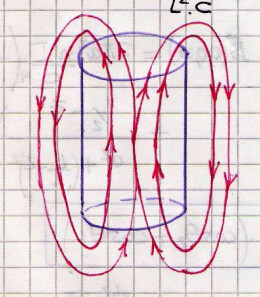
\includegraphics[width=0.2\textwidth]{images/fig_ft1_setproblemasG1_3.jpg}

Si $L \to \infty$ (caso de solenoide infinito) se tiene 
\[
	B_z = \frac{4 \pi n I}{ c },
\]
que es lo mismo que se obtiene haciendo una ley de Ampere.
 
\end{ejemplo}

\begin{ejemplo}{\bf Problema 8}

Acá esto es apenas un comentario.

\notamargen{Para un hilo cargado es $E = 2\lambda /r$}

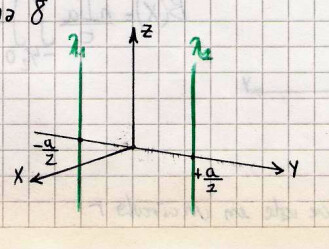
\includegraphics[width=0.3\textwidth]{images/fig_ft1_setproblemasG1_4.jpg} 

\[
	\vb{F}_{12} = \int \rho_1 \vb{E}_1 d\Omega_1 =
	\frac{2 \lambda_2 }{a} \int_\Omega \lambda_1 \delta(x) \delta(y+a/2) d\Omega_1
\]
\[
	\vb{F}_{12} = - \frac{2 \lambda_1 \lambda_2 }{a} L \yver
\]
 
\end{ejemplo}

\begin{ejemplo}{\bf Problema 5}

El potencial
\[
	\phi(r) = \frac{e}{r} \left( 1 + \frac{r}{a} \right) \euler^{-2r/a}
\] 
revienta en cero. No obstante se puede separar en dos potenciales uno de los cuales revienta y el otro no,
\[
	\phi(r) = \frac{e}{r} \euler^{-2r/a} +  \frac{e}{a} \euler^{-2r/a}
\]
donde el primer término es Yukawa, sumando y restando $e/r$ y agrupando
\[
	\phi(r) = \frac{e}{r} \left( \euler^{-2r/a} - 1\right) + \frac{e}{a} \euler^{-2r/a} + \frac{e}{r}
\]
donde el último término es el potencial de una carga en el origen que proviene de una densidad de
carga $\rho = e\delta(\vb{x})$. Definiendo al primer término como $\phi_1$ se puede despejar $\rho$
desde la ecuación de Poisson $ \lapm{\phi} = -4\pi \rho$,
\[
	\rho = -\frac{1}{4\pi r} \frac{1}{r} \dpar[2]{}{r}(r\phi_1)
\]
o bien
\[
	\rho = -\frac{1}{a^2 \pi r} \frac{e}{r} r \euler^{-2r/a}, 
\]
y hemos averiguado la densidad de carga de cada parte.

Entonces, por ser átomo neutro
\[
	Q = \int_V \rho dV + e = 0,
\]
y la integral puede hacerse en esféricas porque la dependencia es solamente en $r$.

\end{ejemplo}




% \bibliographystyle{CBFT-apa-good}	% (uses file "apa-good.bst")
% \bibliography{CBFT.Referencias} % La base de datos bibliográfica

\end{document}

	
		\documentclass[10pt,oneside]{CBFT_book}
	% Algunos paquetes
	\usepackage{amsmath}
	\usepackage{amssymb}
% 	\usepackage{amsbsy}

	\usepackage{graphicx}
% 	\usepackage{bm}
% 	\usepackage{libertine}
% 	\usepackage[bold-style=TeX]{unicode-math}
	\usepackage{lipsum}

	\usepackage{natbib}
	\setcitestyle{square}

	\usepackage{polyglossia}
	\setdefaultlanguage{spanish}


	\usepackage{CBFT.estilo} % Cargo la hoja de estilo

	% Tipografías
	% \setromanfont[Mapping=tex-text]{Linux Libertine O}
	% \setsansfont[Mapping=tex-text]{DejaVu Sans}
	% \setmonofont[Mapping=tex-text]{DejaVu Sans Mono}

	%===================================================================
	%	DOCUMENTO PROPIAMENTE DICHO
	%===================================================================

\begin{document}

% =================================================================================================
\chapter{Teorema de Green}
% =================================================================================================

% =================================================================================================
\section{Imágenes y método de Green}
% =================================================================================================

El método de las imágenes es un procedimiento gráfico de encontrar problemas equivalentes simulando
con cargas extras (cargas imagen) las condiciones de contorno.

\begin{figure}[htb]
	\begin{center}
	\includegraphics[width=0.6\textwidth]{images/fig_ft1_imagegreen1.pdf}	 
	\end{center}
	\caption{}
\end{figure} 

Los problemas que ilustra la figura satisfacen iguales condiciones de contorno en el recinto punteado,
entonces sus soluciones internas son la misma: $\phi_1 = \phi_2$ por unicidad.

\subsection{El Método de Green}

El concepto tras el método de Green es evaluar el $\phi$ de una carga puntual ante cierta configuración
de contornos conductores. Es una excitación elemental.

Restando entre sí
\[
	\Nabla\cdot(\phi\Nabla\psi) = \phi\lapm{\psi} + \Nabla\phi\cdot\Nabla\psi
\]
y
\[
	\Nabla\cdot(\psi\Nabla\phi) = \psi\lapm{\phi} + \Nabla\psi\cdot\Nabla\phi
\]
e integrando ambos miembros y utilizando el teorema de la divergencia, se llega a
\[
	\int_V \left[ \phi\lapm{\psi} - \psi\lapm{\phi}\right] dV =
	\int_S \left[ \phi\Nabla\psi - \psi\Nabla\phi \right] dS,
\]
que es la segunda identidad de Green.

Consideremos lo que llamaremos caso A, según vemos en figura, caracterizado según
\[
	\rho_{int} \qquad \vb{x}'\in R, \vb{x}\in R
\]
\begin{figure}[htb]
	\begin{center}
	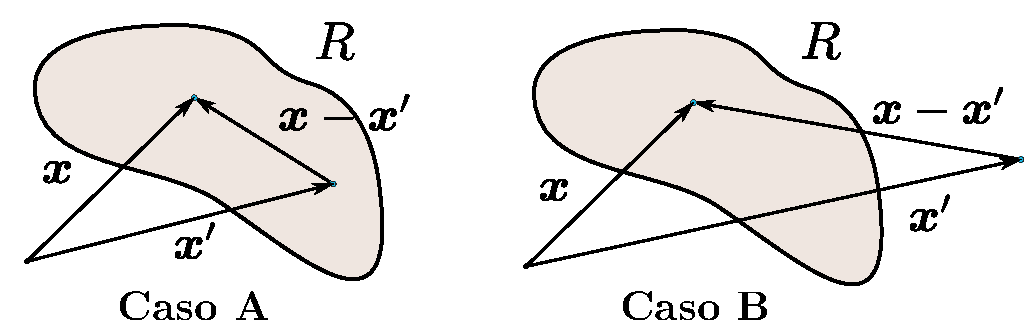
\includegraphics[width=0.8\textwidth]{images/fig_ft1_imagegreenCasos.pdf}	 
	\end{center}
	\caption{}
\end{figure} 
\[
	\psi = \frac{1}{|\vb{x}-\vb{x}'|} \qquad \lapm{\psi} = -4\pi \delta(\vb{x}-\vb{x}')
\]
\[
	-\phi(\vb{x})4\pi + \int_V 4\pi \frac{\rho(\vb{x}')}{|\vb{x}-\vb{x}'|} \; dV' =
	\int_S \left( \phi\dpar{\psi}{n}-\frac{1}{|\vb{x}-\vb{x}'|}\dpar{\phi}{n}\right)\; dS 
\]
donde estamos usando la abreviatura $\Nabla\phi\cdot\vb{n}=\partial\phi/\partial n$ que es la
derivada normal en la superficie. Despejando
\[
	\phi(\vb{x}) = \int_V \frac{\rho(\vb{x}')}{|\vb{x}-\vb{x}'|} \; dV' +
	\frac{1}{4\pi} \int_S \left( \frac{1}{|\vb{x}-\vb{x}'|}\dpar{\phi}{n} -\phi\frac{\partial}{\partial 
n} \left[\frac{1}{|\vb{x}-\vb{x}'|} \right] \right)\; dS ,
\]
donde la primer integral es debido a las cargas internas y la segunda al efecto de las cargas
fuera del reciento $R$.

Recordemos que las condiciones tipo Dirichlet corresponden a $\phi|_S$ y las tipo Neumann a
$\partial\phi/\partial \hat{n}|_S$.

El caso B, según figura, corresponde a
\[
	\rho_{int} \qquad \vb{x}'\notin R, \vb{x}\in R
\]
y 
\[
	\int_V \frac{\rho(\vb{x}')}{|\vb{x}-\vb{x}'|} \; dV' = 
	\frac{1}{4\pi} \int_S \left( \phi\frac{\partial}{\partial n} \left[\frac{1}{|\vb{x}-\vb{x}'|} \right]
	- \frac{1}{|\vb{x}-\vb{x}'|}\dpar{\phi}{n}  \right)\; dS ,
\]
la integral de superficie proviene de las cargas fuera de $R$ que producen campo en el interior
$R$.

Hemos tomado $\psi=1/|\vb{x}-\vb{x}'|$ que verifica [1]; interpretándose $\psi$ como el potencial
de una carga puntual unitaria.

\[
	\lapm{\frac{1}{|\vb{x}-\vb{x}'|}} = - 4\pi \delta( |\vb{x}-\vb{x}'| )
\]
podemos tomar
\[
	G \equiv \frac{1}{|\vb{x}-\vb{x}'|} + f( \vb{x}, \vb{x}')
\]
donde $G$ es la función de Green, el potencial de una carga unidad situada en $\vbx'$ calculado
en $\vbx$.
Luego, se tiene
\[
	\lapm{G} = -4\pi  \delta( \vb{x} - \vb{x}' ) + \lapm{f}
\]
donde $f$ satisface Laplace (si el reciento no incluye a $\vb{x}'$). 
Es decir que $\lapm{f( \vbx, \vbx' )} = 0$.

Entonces $f( \vb{x}, \vb{x}' )$ representan la o las imágenes necesarias para que
$G$ cumpla el contorno necesario $G_D|_S=0$.


% =================================================================================================
\section{Funciones de Green}
% =================================================================================================

El teorema de Green me da una expresión integral para el potencial $\phi$. En efecto,
\be
	\phi(\vb{x}) = \int_{V'} G(\vb{x},\vb{x}') \rho(\vb{x}')  \; dV' +
	\frac{1}{4\pi} \int_{S'} \left( G(\vb{x},\vb{x}')\dpar{\phi(\vbx')}{n} -\phi(\vbx')\frac{\partial}{\partial 
	n} G(\vb{x},\vb{x}') \right)\; dS' ,
	\label{green1}
\ee
y si $\vbx \notin V$, se tiene
\be
	0 = \int_{V'} G(\vb{x},\vb{x}') \rho(\vb{x}')  \; dV' +
	\frac{1}{4\pi} \int_{S'} \left( G(\vb{x},\vb{x}')\dpar{\phi}{n}(\vbx') -\phi(\vbx')\frac{\partial}{\partial 
	n} G(\vb{x},\vb{x}') \right)\; dS' .
	\label{green2}
\ee

Pero para poder utilizar \eqref{green1} necesito tener un solo tipo de condiciones de contorno,
de manera que según sean
\[
	\textrm{Dirichlet} \quad 	\begin{cases}
				G_D : \lapm{G_D} = -4\pi \delta(\vb{x},\vb{x}') \\
				G_D |_{contorno de R} = 0  \\
				\phi|_S \\
				\phi(\vb{x}) = \displaystyle \int_{V'} G_D \rho \; dV' - \frac{1}{4\pi}
				\int_{S} \phi|_S\frac{\partial}{\partial n} G_D \; dS'
			\end{cases}
\]
donde la condición de contorno de $G$ equivale, en el contexto físico del electromagnetismo, a
reemplazar el contorno por un conductor metálico puesto a tierra.
Entonces $G$ es el potencial de la configuración de conductores con el contorno puesto a tierra
frente a una carga puntual con magnitud unitaria.

La función de Green da la geometría del problema.

\[
	\dpar{\phi_1}{n}|_S - \dpar{\phi_2}{n}|_S = -4\pi\sigma \qquad \qquad \phi_2|_S = \phi_1|_S
\]

\[
	\textrm{Neumann} \quad 	\begin{cases}
				G_N : \lapm{G_N} = -4\pi \delta(\vb{x},\vb{x}') \\
				\Nabla G_N \cdot \hat{n}|_S = -\frac{4\pi}{S}  \\
				\left.\dpar{\phi}{n}\right|_S \\
				\phi(\vb{x}) = \displaystyle <\phi>|_S + \int_{V'} G_N \rho \; dV' + 
				\frac{1}{4\pi} \int_{S} G_N|_S \dpar{G_N}{n} \; dS
			\end{cases}
\]

\subsection{Función de Green libre}

La ecuación de Green libre
\[
	G(\vb{x}, \vb{x}') = \frac{1}{|\vb{x} - \vb{x}'|}
\]
que representa una superficie infinita con condición de contorno $\phi(|\vbx| \to \infty) = 0 $
lleva directo a la integral de Poisson. En efecto sería como no tener contornos (tenerlos en
infinito es no tenerlos).
Entonces 
\[
	\phi(\vb{x}) = \int_V G(\vbx,\vbx') \: \rho(\vbx') \:dV = 
	\int_{V'} \frac{ \rho(\vb{x}) }{|\vb{x}-\vb{x}'|} dV'
\]
que es la integral de Poisson. La ecuación de Poisson se recupera teniendo en cuenta
que
\[
	\nabla^2 \left( \frac{1}{|\vb{x} - \vb{x}'|} \right) = 4\pi \delta(\vb{x}-\vb{x}')
\]
% \[
% 	G(\vb{x}, \vb{x}') =  \frac{1}{|\vb{x} - \vb{x}'|} + f(\vb{x}, \vb{x}') \qquad 
% 	\textrm{con} \quad \lapm{f}(\vb{x}, \vb{x}') = 0 \quad \textrm{si} \quad \vb{x}\neq\vb{x}'
% \]
En este caso, Dirichlet y Neumann llevan a la misma solución porque potencial y campo son
nulos en los contornos.

\subsection{Sobre el caso de Neumann}

Para condiciones de Neumann se toma:
\[
	\Nabla G_N|_S = -\frac{4\pi}{S} = \left. \dpar{G}{n} \right|_S
\]
la integral 
\[
	- \frac{1}{4\pi} \int_S \phi|_S \left.\dpar{G}{n}\right|_S  dS
\]
no se puede anular con 
\[
	\left.\dpar{G}{n}\right|_S = 0
\]
salvo que el volumen de integración no contenga a $\vb{x}=\vb{x}'$ en cuyo caso:
se excluye $\vb{x}=\vb{x}'$ de la integración.
\[
	- \frac{1}{4\pi} \int_S \phi|_S \left.\dpar{G}{n}\right|_S  dS =
	\frac{1}{S} \int_S \phi|_S dS = <\phi>|_S
\]
que es el valor promedio de $\phi$ en la superficie $S$.

Se suele tomar la superficie $S \to \infty$ de modo que resulte nulo $<\phi>|_S$.
Se toma el volumen $V$ rodeado por dos superficies una cerrada y finita y la otra
en infinito entonces
\[
	<\phi>|_S = 0 \qquad \qquad \left. \dpar{G}{n}\right|_S = 0
\]
esto es el llamado {\it problema exterior}.

\subsection{Green para el problema externo de una esfera}

\notamargen{Este título sería ``Ejemplo método de imágenes''. En realidad este es un ejemplo
de cálculo de función de Green; así fue dado en la teoría.}

La configuración es una carga puntual $q$ frente a una esfera metálica de radio $a$ conectada a tierra.
La idea aquí es conocer dónde ubicar la imagen $ q' $ para que se verifique el contorno, es decir que
el potencial será ahora el correspondiente a las dos cargas 
\[
	\vp(\vbx) = \frac{q}{|\vbx - \vb{y}|} + \frac{q'}{|\vbx - \vb{y}'|} 
\]
y debe cumplir que 
\[
	\left. \vp(\vbx)\right|_{r=a} = 0,
\]
por la conexión a tierra. Para ajustar esta condición se tienen dos variables, la magnitud de la carga
$q'$ y su posición $\vb{y}'$.
No obstante, la simetría de la configuración establece ciertas restricciones para la posición $\vb{y}'$;
en efecto para el problema de una carga frente a una esfera el eje que une el centro de la esfera con
la carga es un eje de simetría de revolución; si la esfera gira en torno a ese eje la configuración es
la misma. Luego, la carga imagen debe ser tal que no rompa esa simetría: debe estar localizada en dicho
eje. Entonces $\vb{y}'$ y $\vb{y}$ son colineales y la posición incógnita requerida es solamente el
módulo $y'= |\vb{y}'|$.

Los módulos en los denominadores pueden expresarse en términos de la ley de los cosenos, como
\[
	\vp(\vbx) = \frac{q}{\sqrt{ x^2 + y^2 - 2 \: x \: y \:\cos{\gamma}} } +
	\frac{q'}{\sqrt{ x^2 + y'^2 - 2 \: x \: y' \cos{\gamma} }},
\]
donde $x, y$ son los módulos respectivos.

\begin{figure}[!htb]
	\begin{center}
	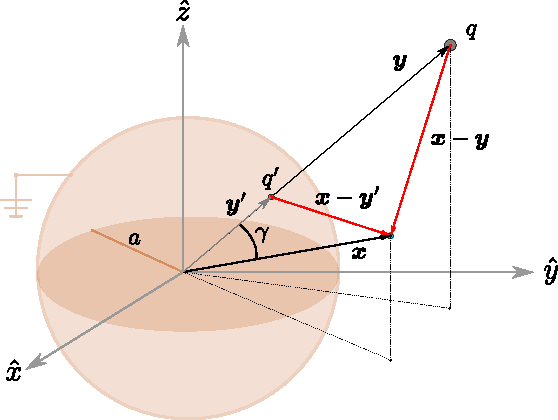
\includegraphics[width=0.5\textwidth]{images/fig_ft1_esfera_imagenes.pdf}
	\end{center}
	\caption{Geometría para el problema de la carga puntual $q$ frente a una esfera
	metálica de radio $a$ conectada a tierra.}
\end{figure} 

Luego, la condición de contorno evaluada sobre la superficie de la esfera $|\vb{x}| = a$ implica que 
\[
	\left. \vp(\vbx)\right|_{|\vb{x}| = a} = 
	\frac{q}{\sqrt{ a^2 + y^2 - 2 \: a \: y \:\cos{\gamma}} } +
	\frac{q'}{\sqrt{ a^2 + y'^2 - 2 \: a \: y' \: \cos{\gamma} }} = 0,
\]
y entonces se tienen que obtener ahora $q, y'$ a partir de esta ecuación que en realidad representan
infinitas direcciones dado que $ \gamma $ puede ser cualquier ángulo entre $0$ y $2\pi$.
Se necesitarán dos ecuaciones para resolver unívocamente el problema.
Si se eligen $\gamma = \pi$ y $\gamma = 0$ la ecuación anterior define el sistema
\notamargen{Parece ser una constante que si elegimos las cosas del modo más simétrico posible, las
expresiones resultan más sencillas.}
\[
	\begin{cases}
		\displaystyle \frac{q}{y-a} + \frac{q'}{a-y'} = 0 \\
		\\
		\displaystyle  \frac{q}{a+y} + \frac{q'}{a+y'} = 0 
	\end{cases}
\]
cuya solución es el par
\[
	q' = - \frac{a}{y} \: q, \qquad y' = \frac{a^2}{y},
\]
y entonces
\[
	\vp(\vbx) = \frac{q}{\sqrt{ x^2 + y^2 - 2 \: x \: y \:\cos{\gamma}} } -
	\frac{ ( a / y ) \: q }{ \sqrt{ x^2 + a^4 / y^2  - 2 \: x \:  ( a^2 / y ) \cos{\gamma} }}.
\]
El potencial en un punto $\vbx$ del espacio, debido a una carga en $\vb{y}$ depende de los módulos $x, y$ 
y del ángulo $\gamma$ entre dichos vectores.
\notamargen{Esta expresión, así como está, no se halla en ningún sistema de coordenadas en particular.}

Esta solución puede obtenerse un poco más heurísticamente, ver nota \ref{notas_carga_frente_a_esfera}.

Lo que sucede físicamente es que se induce carga sobre la superficie de la esfera.
Se querrá ver (luego?) cuál es la distribución de carga que se inducirá sobre la superficie.


\begin{figure}[htb]
	\begin{center}
	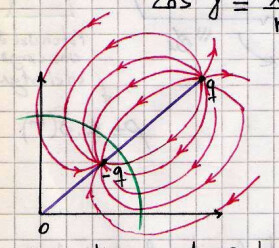
\includegraphics[width=0.4\textwidth]{images/fig_ft1_carga_induciendo_en_esfera.jpg}	 
	\end{center}
	\caption{}
\end{figure}

Este ejemplo ha servido también para mostrar la determinación de la funcion de Green para la configuración
dada por una esfera aterrizada (condiciones de Dirichlet), que sería
\[
	G(\vbx,\vb{y}) = \frac{1}{| \: \vbx - \vb{y} \:|} - \frac{a/|\vb{y}|}{| \:\vbx - ( a^2 / |\vb{y}| ) \hat{y} \: |} 
\]

% En este problema las condiciones adecuadas son las de Dirichlet, ver Figura,
% y podemos escribir la función de Green como 
% \[
% 	G = \frac{1}{|\vb{r} - D\hat{r}'|} - \frac{a/D}{|\vb{r} - a^2/D\hat{r}'|} \qquad G|_{r=a}
% \]
% sujeta a que 
% \[
% 	q' = -q a/D \qquad d = a^2/D
% \]
\begin{figure}[htb]
	\begin{center}
	\includegraphics[width=0.6\textwidth]{images/fig_ft1_green2.pdf}	 
	\end{center}
	\caption{$G_D$ es el potencial de la configuración (a) y se evalúa teniendo en cuenta la
	otra (b) que se resuelve casualmente por imágenes. La (c) se resuelve alterando las condiciones.}
\end{figure} 

El caso (c) de la Figura se resuelve con 
\[
	-\frac{V}{4\pi} \int_S \dpar{G}{n} dS = -\frac{V}{4\pi} \int_S \Nabla G\cdot d\vb{S} =
	-\frac{V}{4\pi} \int_V \lapm{G} \: dV	
\]
\[
	= -\frac{V}{4\pi} (-4\pi)\int_V \delta(\vb{x}-\vb{x}') \: dV	= V 
\]

\subsection{Algunos campos}

En distribuciones infinitas de carga la integral de Poisson diverge pero ello se debe a que en
realidad no existen distribuciones infinitas de carga.
% \begin{figure}[thb]
% 	\begin{center}
	\includegraphics[width=0.8\textwidth]{images/fig_ft1_campohilos.pdf}	 
% 	\end{center}
% 	\caption{}
% \end{figure} 

\begin{ejemplo}{\bf Problema 1}

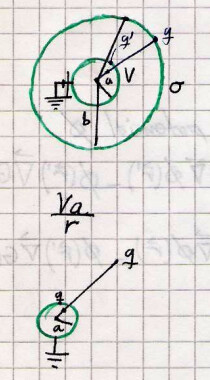
\includegraphics[width=0.2\textwidth]{images/fig_ft1_g1_p1_A.jpg} 

Primeramente se calculan los valores de la carga imagen, los cuales, para un
sistema de coordenadas esféricas, son
\[
	q'= -\frac{a}{r} q \qquad r'= \frac{a^2}{r}.
\]
Se ve que cumplen los límites razonables.
Luego, habría que hacer el potencial nulo mandando el engendro a tierra y luego se
le suma algo que de potencial $V$ en $r=a$.

La función de Green por imágenes será
\[
	G_D = \frac{1}{|\vbx - \vbx'|} - \frac{1}{r'|\vbx - a^2/r'^2 \vbx'|},
\]
la cual cumple que sobre la superficie es nula.

Subsecuentemente,
\[
	\rho(\vbx') = \sigma \delta(r-b), \phi(\vbx')|_S = V, \phi(\vbx')|_{S_{R\to\infty}} = 0 
\]
y
\[
	\int \rho(\vbx') \: dV = 4 \pi b^2 \sigma 
\]
\[
	\int \rho(\vbx') \: G_D( \vbx, \vbx')  \: dV = \int \frac{b^2 \sigma}{|\vbx - \vbx'|} \: dS
\]
siendo $b=|\vbx'|$. Poniendo manos a la obra en la integral (en esféricas)
\[
	\int \frac{b^2 \sigma}{|\vbx - \vbx'|} \: dS =
	\int dt \int d\Omega r^2 \sigma \delta(r'-b) 
	\left[ \frac{1}{|\vbx - \vbx'|} - \frac{1}{r'|\vbx - a^2/r'^2 \vbx'|} \right]
\]
\[
	\int d\Omega \sigma b^2
	\left[ \frac{1}{|\vbx - \vbx'|} - \frac{1}{r'|\vbx - a^2/r'^2 \vbx'|} \right]
\]
donde el primer término es el potencial de un casquete, que es 
\[
	\begin{cases}
	 \displaystyle \frac{4\pi b^2\sigma}{r} \quad \text{ si } \; r > b \\
	 \\
	 \displaystyle 4 \pi b^2 \sigma \quad \text{ si } \; a < r < b 
	\end{cases}
\]
y el segundo término se puede trabajar para llegar a
\[
	\frac{b^2 a }{r} \int d\Omega \sigma \frac{-1}{|a^2/r^2 \vbx - \vbx'|} 
\]
Pero recordemos que 
\[
	\dpar[2]{\vbx}{r} = \frac{a^2}{r} < a
\]

Juntando todo
\[
	\begin{cases}
	 \displaystyle \frac{4\pi b^2\sigma}{r} - \frac{a}{r} 4 \pi \sigma b \qquad \text{ si } \; r > b \\
	 \\
	 \displaystyle  4 \pi b^2 \sigma - \frac{a}{r} 4 \pi \sigma b \qquad \text{ si } \; a < r < b  
	\end{cases}	
\]

Y se tiene 
\[
	-\frac{ 1 }{ 4\pi } \int \phi(\vbx') \Nabla' G_D(\vbx,\vbx') dS' =
	\frac{ V }{ 4 \pi } \int \Nabla' G_D(\vbx,\vbx') dS' = V Q_n,
\]
donde en el último paso se ha usado el teorema de la divergencia. Luego, como
$Q_n = -a/r$ se tiene 
\[
	\phi = \frac{Va}{r}
\]
que entonces en $r=a$ es $V$.

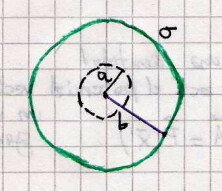
\includegraphics[width=0.2\textwidth]{images/fig_ft1_g1_p1_B.jpg} 

Esto conviene hacerlo integrando en esféricas con $\vbx \parallel \hat{z}$.

\end{ejemplo}

\begin{ejemplo}{\bf Comentario superposición}
 
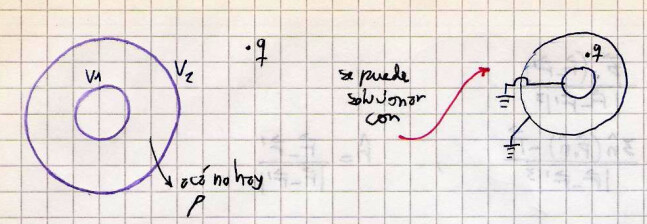
\includegraphics[width=0.5\textwidth]{images/fig_ft1_comentario_superposicion.jpg} 
 
\end{ejemplo}

% =================================================================================================
\section{Condiciones de contorno para el campo eléctrico}
% =================================================================================================

Consideraremos la superficie de separación entre dos medios 1 y 2, la cual puede estar cargada, y sobre
la misma imaginaremos un cilindro pequeño $\Sigma$ de tapas paralelas a la superficie y altura despreciable y 
asimismo, un circuito cerrado $\Gamma$ también de altura despreciable perpendicular a la superficie, ver figura.

La normal a la superficie es $\hat{n}$ mientras que $\hat{t}$ es un versor tangente a la misma.

\begin{figure}[!htb]
	\begin{center}
	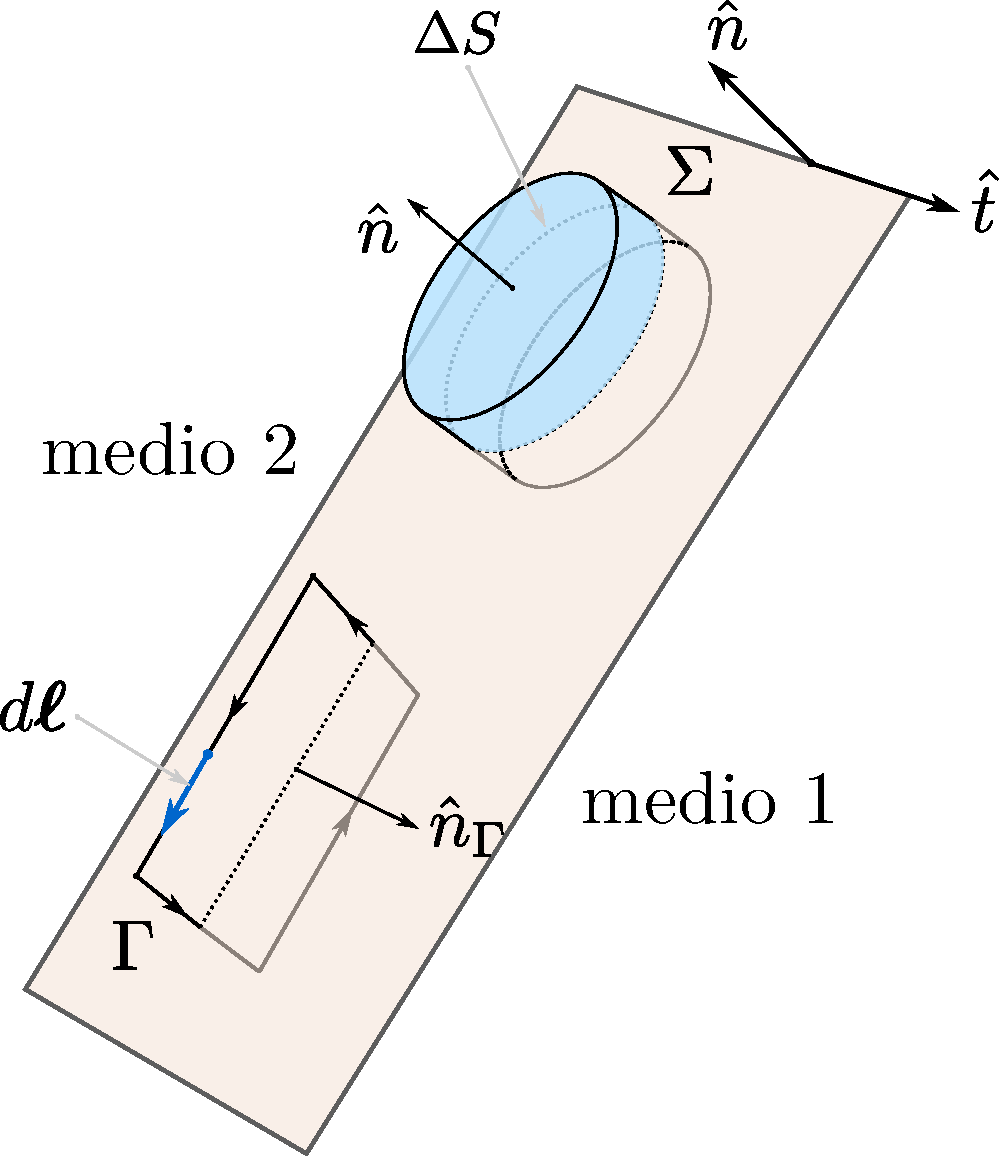
\includegraphics[width=0.4\textwidth]{images/fig_ft1_contornos_E.pdf} 
	\end{center}
	\caption{}
\end{figure} 

La ley de Gauss establece para el cilindro $\Sigma$ que 
\[
	\int_{S_\Sigma} \vb{E} \cdot d\vb{S} = 4 \pi \: Q_n,
\]
donde $ {S_\Sigma}$ es la superficie total del cilindro y $Q_n$ la carga neta encerrada.
Como la superficie lateral es despreciable, por serlo la altura, la integral de superficie se reduce a la
de las tapas. Si la densidad de carga sobre la superficie es $\sigma$ entonces
\[
	( \vb{E}_2 - \vb{E}_1 )\cdot \hat{n} \: \Delta S = 4 \pi \: \sigma \: \Delta S 
\]
o bien
\[
	( \vb{E}_2 - \vb{E}_1 )\cdot \hat{n} = 4 \pi \sigma 
\]
lo cual implica que la componente normal del campo $\vb{E}$ es discontinua si hay carga superficial presente.

\notamargen{No sé si no decir directamente que en electrostática es nula la integral de línea de E y ya.}
Por otra parte, como el rotor de $\vb{E}$ es nulo (en electrostática), el teorema de Stokes implica
\[
	\int_{S} \: \rotorm{E} = 0 = \int_{\Gamma} \vb{E} \cdot d\Bell
\]
y despreciando el aporte de las partes del circuito que son perpendiculares a la superficie, resulta
\[
	( \vb{E}_2 - \vb{E}_1 ) \cdot d\Bell  = 
	( \vb{E}_2 - \vb{E}_1 ) \cdot ( \hat{n}_\Gamma \times \hat{n} ) \: d\ell = 0
\]
donde en el miembro derecho se ha expresado la dirección del $d\Bell$ en función de los versores
normal y tangencial, y entonces
\[
	\hat{n}_\Gamma \cdot ( \hat{n} \times  ( \vb{E}_2 - \vb{E}_1 ) ) = 0,
\]
que indica que el segundo factor tiene que ser nulo, es decir 
\[
	 \hat{n} \times  ( \vb{E}_2 - \vb{E}_1 ) = 0
\]
y esto implica que la componente tangencial del campo es continua, sin importar que exista carga o no.
\notamargen{Acordate que harcodeaste con un pdf el $\ell$ bold.}

Entonces el trabajo yendo del medio 1 al 2 será nulo
\[
	W_{1\to 2} = 0 = q ( \phi_2 - \phi_1 ),
\]
lo cual implica que $\phi_2 = \phi_1$ porque la discontinuidad del campo es finita.
Como veremos luego, esto no vale en el caso de una capa dipolar.
\notamargen{Hay que ver la relación de esto con lo anterior; creo que no estoy entendiendo, o explicando,
bien.}

Resumiendo
\[
	E_{2\hat{n}} - E_{1\hat{n}} = 4 \pi \sigma \qquad \qquad E_{2\hat{t}} -E_{1\hat{t}} = 0
\]

Expresando el campo en términos del potencial, se tiene
\[
	-\Nabla\phi_2\cdot\hat{n} + \Nabla\phi_1\cdot\hat{n} = 4 \pi \sigma
\]
\[
	\frac{\Nabla(\phi_2-\phi_1)\cdot \hat{n}}{4 \pi} = \sigma
\]
\be
	\sigma = \frac{1}{4\pi}\dpar{(\phi_1-\phi_2)}{n}
	\label{densidad_de_carga}
\ee
esta es la densidad de carga inducida sobre la frontera entre medios.

\subsection{Carga puntual frente a esfera puesta a tierra}

Volvemos a este problema, recordando que el potencial fuera de la misma se hubo determinado por el método
de imágenes. Recordemos también que dentro de la esfera el potencial debe ser constante (no hay carga allí,
puesto que la imagen es un dispositivo virtual sin existencia física).
Consideramos dos secciones, interna y externa.

Por la simetría del problema la densidad de carga inducida tiene la simetría de revolución en torno al 
eje que pasa por $q, q'$ y el origen de coordenadas y será máxima en el punto de la esfera más cercano a
$q$.
Dado que el potencial es constante dentro de la esfera, e igual al valor que toma sobre la superficie, la
ecuación \eqref{densidad_de_carga} es 
\[
	\sigma = - \frac{1}{4\pi} \left.\dpar{\vp}{n}\right|_S.
\]
Ubicando nuestra esfera en el origen de un sistema de coordenadas esféricas, la normal externa $\hat{n}$
es claramente $\rver$ de modo que derivar normalmente es derivar con respecto a la dirección radial, es 
decir $\partial / \partial n \equiv \partial / \partial r$ y entonces 
\[
	\sigma = - \frac{1}{4\pi} \left.\dpar{\vp}{r}\right|_{r=a} =
	- \frac{q}{4 \pi a^2} \Frac{a}{y} 
	\frac{[ 1 - (a / y)^2 ]}{[\: 1 + (a / y)^2 - 2 \: (a/y) \: \cos \gamma \:]^{3/2}}.
\]
\notamargen{La definición de derivada normal puede ir para apéndice.}

Si consideramos ahora el problema interno; esto es, una carga q rodeada por una esfera conductora conectada
a tierra, se pueden hacer los mismos razonamientos que en el caso de la carga exterior y la solución es la
misma intercambiando $q'$ por $q$ y $y'$ por $y$.
Entonces, en ese caso el cálculo de la densidad utiliza $\hat{n} = -\rver$ y se tiene 
\[
	\sigma = \frac{1}{4\pi} \left.\dpar{\vp}{r}\right|_{r=a} =
	- \frac{q}{4 \pi a^2} \Frac{a}{y} 
	\frac{[ (a / y)^2 - 1 ]}{[\: 1 + (a / y)^2 - 2 \: (a/y) \: \cos \gamma \:]^{3/2}}
\]
\notamargen{Acá debiera estar claro que se invierte el significado de $y'$, ahora es mayor que $a$.}

La carga total inducida sobre una superficie se evaluará en general a través de
\[
	Q = \int_S \: \sigma \: dS.
\]

En el caso anterior del problema de la carga frente a una esfera a tierra se puede utilizar la ley de Gauss
para hallar en cada caso la carga total de una manera inmediata.

% \begin{figure}[hb]
% 	\begin{center}
	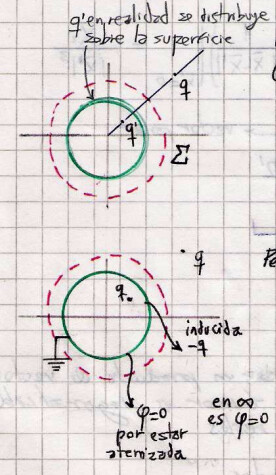
\includegraphics[width=0.25\textwidth]{images/fig_ft1_calculo_carga_fast.jpg}	 
% 	\end{center}
% 	\caption{}
% \end{figure} 

Situando una superficie gaussiana $\Sigma$ por fuera de la esfera, como se ve en la figura, resulta que la
carga encerrada neta es la misma con imagen o sin imagen. En efecto, en el problema real la carga encerrada
se distribuye sobre la superficie mientras que en el problema equivalente está concentrada en la posición
$y'$ y sabemos que es $q'$; luego como los dos problemas son equivalentes el lado derecho de la ley de 
Gauss debe ser idéntico y la carga inducida será la neta encerrada, que es $q'$, la carga imagen.

Procediendo de modo similar para el problema interno (ahora $q'$ está por fuera de la superficie $\Sigma$),
ahora la situación es diferente porque el campo sobre \Sigma es nulo (solo es no nulo fuera de la esfera
por la conexión a tierra). Entonces la ley de Gauss ya nos dice ahí que la carga neta es nula y ello
lleva a que la carga inducida sea $-q$ que no es igual a la carga imagen.


\subsection{Principio de superposición}

Consideremos la situación depicted en la figura

\begin{figure}[htb]
	\begin{center}
	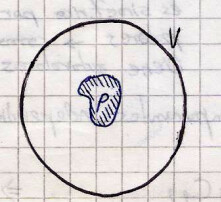
\includegraphics[width=0.2\textwidth]{images/fig_ft1_rho_rodeada_por_V.jpg}	 
	\end{center}
	\caption{}
\end{figure} 

Una cierta distribución de carga está rodeada por una superficie a potencial $V$.
El potencial en un punto $\vbx$ es
\[
	\vp(\vbx) = \int_\Omega \rho(\vbx') \: G_D(\vbx,\vbx') \: d\Omega 
	- \frac{1}{4\pi} \int \vp \dpar{G}{n} \: dS
\]
pero como el potencial sobre la superficie está fijo en $V$ la última integral es 
\[
	- \frac{1}{4\pi} \int \vp \dpar{G}{n} \: dS = - \frac{V}{4\pi} \int \Nabla G \cdot\hat{n} \: dS,
\]
la cual por el teorema de la divergencia resulta
\[
	- \frac{V}{4\pi} \int \Nabla G_D \cdot\hat{n} \: dS =
	- \frac{V}{4\pi} \int_V \Nabla \cdot (\Nabla G_D) \: dV =
	- \frac{V}{4\pi} \int_V \lapm{G_D} \: dV
\]
y recordando que la función de Green es solución de la ecuación de Poisson para una densidad dada por
la delta de Dirac, se tiene
\[
	- \frac{V}{4\pi} \int \Nabla G_D \cdot\hat{n} \: dS = 
	V \int \delta(\vbx - \vbx') \: dV = V,
\]
de manera que 
\[
	\vp{\vbx} = \int_\Omega \rho(\vbx') \: G_D(\vbx,\vbx') \: d\Omega  + V,
\]
lo cual puede una manera de ver el principio de superposición.


\textbf{Notas importantes sobre el principio de superposición}

La ecuación de Poisson es muchas veces inútil porque en general no se tiene la distribución de cargas
$ \rho(\vbx) $. Esto sucede en general con conductores pués la carga allí se distribuye acomodándose
para alcanzar el equilibrio.

Para campos y potenciales vale superposición.
Pero cada problema de potencial (con su ecuación de poisson) incluye además de la ecuación las condiciones
de contorno. 
Dados dos problemas
\[
	\nabla^2 \vp_1 = - 4 \pi \rho_1 \qquad + \qquad \text{CC}_1
\]
y
\[
	\nabla^2 \vp_2 = - 4 \pi \rho_2 \qquad + \qquad \text{CC}_2
\]
la suma de soluciones $ \vp = \vp_1 + \vp_2 $ con $\rho = \rho_1 + \rho_2 $
\be
	\nabla^2 \rho = - 4 \pi \rho \qquad + \qquad \text{CC}
	\label{problema_potencial_suma}
\ee
donde hay que asegurarse de que $ \text{CC} $ sea la suma de las condiciones del problema 1 y las del
problema 2.
Desde el otro punto de vista, si tengo un problema como \eqref{problema_potencial_suma} y lo quiero
pensar como la superposición de dos potenciales $ \vp = \vp_1 + \vp_2 $ puedo generarme unas condiciones
de contorno artificiales que tengan en cuenta las influencias mutuas.

\notamargen{Habría que entender bien este tema que es crucial. Imagino que working los ejemplos podría
recuperar lo que alguna vez supe.}

\subsection{Condiciones de contorno para medios magnéticos}

Para los medios magnéticos
\[
	\rotorm{H} = \frac{4 \pi}{c} \vb{J}_l
\]
\[
	\int_S (\rotorm{H}) \cdot d\vb{S} = \int_S \frac{4 \pi}{c} \vb{J}_l \cdot d\vb{S} = 
	\frac{4 \pi}{C} \vb{g}_l\cdot \hat{s} d\ell
\]
donde hicimos la transformación
\[
	\int \vb{H}\cdot d\ell = (\vb{H}_2-\vb{H}_1)\cdot d\ell
\]
y donde recordemos que la altura de $\Gamma$ tiene a cero.
\[
	\frac{4 \pi}{c} \vb{g}_l \cdot \vb{s} = ( -\vb{H}_2 + \vb{H}_1 )\cdot( \hat{n} \times \hat{s} ) d\ell
\]
\[
	\frac{4 \pi}{c} \vb{g}_l \cdot \vb{s} \; d\ell = (\vb{H}_1 -\vb{H}_2 \times \hat{n})\cdot \hat{s} 
d\ell
\]

\begin{figure}[htb]
	\begin{center}
	\includegraphics[width=0.4\textwidth]{images/fig_ft1_contorno2.pdf}	 
	\end{center}
	\caption{}
\end{figure} 

de manera que 
\[
	\frac{4 \pi}{c} \vb{g}_l = \hat{n} \times ( \vb{H}_2 - \vb{H}_1 )
\]
\[
	\hat{n}\times\hat{s} = \frac{d\vb{\ell}}{d\ell} 
\]
\[
	B_{2\hat{n}} - B_{1\hat{n}} = 0 \qquad \qquad H_{2\hat{t}} - H_{1\hat{t}} = \frac{4 \pi}{c} g_l
\]
\[
	\int_S \vb{B}\cdot d\vb{S} = 0 \Rightarrow (\vb{B}_2 - \vb{B}_1 )\cdot\hat{n} = 0
\]

% =================================================================================================
\section{Desarrollo multipolar}
% =================================================================================================

Si se conoce la distribución de carga el potencial se obtiene integrando
\be
	\phi(\vb{x}) = \int_{V'} \frac{ \rho( \vbx' ) }{| \vbx -\vbx' | } \; dV'.
	\label{integral_potencial}
\ee

No obstante, esta expresión puede ser muy complicada porque en el denominador depende de la variable 
$\vbx'$ sobre la cual se está integrando. 
Resulta conveniente entonces hacer un desarrollo del denominador, que es una función de $\vbx'$, en
torno a un punto que se toma como origen de una esfera que engloba a la distribución de carga.
Luego, ese dearrollo será válido en puntos externos a dicha esfera.

\notamargen{Se necesita una serie que converja, y que lo haga rápido.
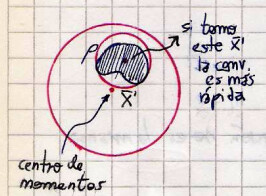
\includegraphics[width=0.3\textwidth]{images/fig_ft1_expansion_multipolar.jpg}}

Entonces, desarrollando en torno a $\vbx'=0$ (el origen de coordenadas) se tienen
\[
	\frac{ 1 }{| \vbx -\vbx' | } = 
	\frac{ 1 }{| \vbx |} + \left.\partial_i \left( \frac{ 1 }{| \vbx -\vbx' | } \right)\right|_{\vbx'=0} x_i' +
	\frac{1}{2} \: \left. \partial_j \partial_i \left( \frac{ 1 }{| \vbx -\vbx' | } \right)\right|_{\vbx'=0} x_i' x_j' + ...,
\]
o bien 
\[
	\frac{ 1 }{| \vbx -\vbx' | } = 
	\frac{ 1 }{| \vbx |} + \frac{x_i \: x_i'}{| \vbx |^3} +
	\frac{1}{2} \frac{ x_i \: x_i' \: x_j \: x_j' }{ | \vbx |^5 } + ...,	
\]
\notamargen{Chequear la expansión, tal vez ponerla en vectorial o hacerla bien en el Apéndice.
Juntar huevos y hacer el término siguiente.}
Luego, introduciendo la misma en \eqref{integral_potencial} resulta
\begin{multline*}
 	\phi(\vb{x}) =
	\frac{ 1 }{| \vbx |} \int_{V'} \rho( \vbx' ) \: dV' + 
	\frac{x_i }{| \vbx |^3} \: \int_{V'} \: x_i' \: \rho( \vbx' ) \: dV' + \\
	\frac{1}{2} \frac{ x_i  \: x_j  }{ | \vbx |^5 } 
	\int_{V'} \: (\: 3 x_i' \: x_j' - \delta_{ij}|\vbx|^2 \:) \: \rho( \vbx' ) \: dV' + ...,
\end{multline*}
% \[
% 	\phi(\vb{x}) =
% 	\frac{ 1 }{| \vbx |} \int_{V'} \rho( \vbx' ) \: dV' + 
% 	\frac{x_i }{| \vbx |^3} \: \int_{V'} \: x_i' \: \rho( \vbx' ) \: dV' +
% 	\frac{1}{2} \frac{ x_i  \: x_j  }{ | \vbx |^5 } 
% 	\int_{V'} \: (\: 3 x_i' \: x_j' - \delta_{ij}|\vbx|^2 \:) \: \rho( \vbx' ) \: dV' + ...,
% \]

Se tiene un desarrollo de diferentes órdenes 
\[
	\phi(\vb{x}) = \phi^{(0)}(\vbx) + \phi^{(1)}(\vbx) + \phi^{(2)}(\vbx) + \phi^{(3)}(\vbx) + ...
\]
que se conocen según
\[
	\frac{ 1 }{| \vbx |} \int_{V'} \rho( \vbx' ) \: dV' = \frac{ Q }{| \vbx |} \qquad \text{ Orden monopolar }
\]
\[
	\frac{x_i }{| \vbx |^3} \: \int_{V'} \: x_i' \: \rho( \vbx' ) \: dV' = 
	\frac{x_i \: p_i }{| \vbx |^3} \: \qquad \text{ Orden dipolar }
\]
\[
	\frac{1}{2} \frac{ x_i  \: x_j  }{ | \vbx |^5 } 
	\int_{V'} \: (\: 3 x_i' \: x_j' - \delta_{ij}|\vbx|^2 \:) \: \rho( \vbx' ) \: dV' =
	\frac{1}{2} \frac{ x_i  \: Q_{ij} \: x_j  }{ | \vbx |^5 } \qquad \text{ Orden cuadrupolar }
\]
% \[
% 	\qquad \text{ Orden octupolar }
% \]

El último término, matricialmente sería
\[
	\frac{1}{2} \frac{\vb{x}^t Q \vb{x}}{|\vb{x}|^5}.
\]

Los momentos son el momento monopolar,
\[
	Q = \int_V \rho(\vb{x}) dV, 
\]
que es la carga total, el momento dipolar,
\[
	\vb{p} = \int_V \vb{x} \: \rho(\vb{x}) \: dV
\]
y el momento cuadrupolar
\[
	Q_{ij} = \int_V  \rho(\vb{x}) \left[ 3 x_i x_j - \delta_{ij} |\vb{x}|^2 \right] \: dV
	= 3 \int_V  \rho(\vb{x}) x_i \: x_j  \: dV - \delta_{ij} \int_V  \rho(\vb{x})  |\vb{x}|^2  \: dV
\]
\[
	Q_{ij} = 3 C_{ij} - \delta_{ij} C_{ll},
\]
donde esta última expresión permite ver que el momento cuadrupolar es de traza nula ($C_{ll}$ es la traza).

El momento cuadrupolar refleja apartamiento de la esfera perfecta, los momentos dipolar y cuadrupolar
indican desbalance de carga.
Asimismo $Q_{ij} = Q_{ji}$ es simétrico por ser producto de vectores polares.
Es siempre diagonalizable y tiene autovalores reales. 
Tiene traza nula,
\[
	Q_{xx} + Q_{yy} + Q_{zz}  = 0
\]

El tensor diagonalizado tendrá tres componentes independientes.


Se da también que $Q_{ij} (i\neq j)$ mide desbalance lejos de los ejes.
Una esfera con $\rho$ uniforme tiene todos los momentos multipolares nulos salvo el monopolo.

\begin{figure}[htb]
	\begin{center}
	\includegraphics[width=0.8\textwidth]{images/fig_ft1_multipolo2.pdf}	 
	\end{center}
	\caption{}
\end{figure}

\notamargen{El comentario en pag. 12 de la carpeta -recuadrado en rojo- induce algo diferente;
pide simetría en el plano perpendicular al vector. Me parece a mí que lo que debiera verse es
una simetría en la distribución de carga.}
Una simetría de reflexión implica que el $\vb{p}_\perp = 0$ donde la notación significa perpendicular
al plano. Esto es así porque no hay desbalance. Para una simetría de revolución $Q_{xx}=Q_{yy}$ entonces
el $Q_{ij}$ puede darse con un sólo número.

Si en una distribución dada, los momentos multipolares hasta el orden $\ell -1$ son nulos entonces
el momento multipolar de orden $\ell$ no depende del origen de coordenadas.
Así, por ejemplo, cuando el monopolo es nulo el momento dipolar no depende del centro de momentos.

\begin{figure}[htb]
	\begin{center}
	\includegraphics[width=0.6\textwidth]{images/fig_ft1_multipolo3.pdf}	 
	\end{center}
	\caption{}
\end{figure}

En la figura vemos que no ambos no tienen desbalance de carga respecto del origen; el disco uniformemente
cargado tendrá monopolo no nulo y dipolo nulo (siempre respecto del origen), los anillos cargados con carga
opuesta tendrán monopolo y dipolo nulos (respecto del origen y de cualquier otro punto). Pero si muevo las
distribuciones se tendrá desbalance el disco pero no los anillos.

\begin{figure}[htb]
	\begin{center}
	\includegraphics[width=0.3\textwidth]{images/fig_ft1_multipolo4.pdf}	 
	\end{center}
	\caption{}
\end{figure}

Para átomos en general son monopolo, dipolo neutros; el cuadrupolo se da con un solo número. 
En la Figura tenemos un elipsoide con densidad de carga $\rho$ uniforme. Tiene simetría de revolución
de modo que el momento cuadripolar es un número. $Q_{zz} = 0 $ puesto que una esfera no tiene
desbalance, entonces $\overleftrightarrow{Q} = 0 $ 

Para una esfera uniformemente cargada todos los momentos dipolares más allá del monopolo valen
cero, lo cual se ve por ley de Gauss.

En general en las aplicaciones uno se queda con tres términos; monopolo, dipolo y cuadrupolo y se
busca que esa expresión converja rápido. En general tomando como centro el centro de la distribución
la convergencia es más rápida.


% =================================================================================================
\section{Dipolo eléctrico}
% =================================================================================================

Se obtiene como límite de 
\[
	\phi(\vb{x}) = \frac{ q }{| \vbx - \vbx_+ |}  - \frac{ q }{| \vbx - \vbx_- |}.
\]
\notamargen{No sé si corresponde hacer mención a que el potencial del dipolo se obtiene como 
límite en el caso de que la distancia entre cargas tiende a la nulidad.}

El potencial de un dipolo es
\[
	\phi(\vb{x}) = \frac{ \vb{p}\cdot\vb{x} }{|\vb{x}|^3} 
\]
si está en el origen, y
\[
	\phi(\vb{x}) = \frac{ \vb{p}\cdot(\vb{x}-\vb{x}_0) }{|\vb{x} - \vb{x}_0|^3} 
\]
si está en un punto $\vb{x}_0$. Para calcular el campo hay que tomar el gradiente de esta expresión,
multiplicarlo por $-1$, lo cual es un poco trabajoso, pero ahí vamos.
Usando que el segundo miembro es a su vez un gradiente [poner esa cuenta en el apéndice matemático]
se tiene 
\[
	\vb{E}(\vb{x}) = -\Nabla \phi(\vbx) = 
	-\Nabla \left( \frac{ \vb{p}\cdot(\vb{x}-\vb{x}_0) }{|\vb{x} - \vb{x}_0|^3} \right) =
	\Nabla \left( \vb{p} \cdot \Nabla\left( \frac{ 1 }{|\vb{x} - \vb{x}_0|} \right) \right),
\]
luego se utiliza la identidad para el gradiente de un producto escalar notando que como uno de
los vectores en el escalar es a su vez un gradiente se tiene una expresión más sencilla 
[otra cuenta de apéndice]
\notamargen{La identidad es $\Nabla(\pe{A}{B}) =$ cuatro términos, dos rotores y dos
términos del tipo convectivo.}
En efecto, el primer término se anula por involucrar el producto vectorial de un gradiente, el
segundo y tercero porque $\vb{p}$ es independiente de $\vbx$ reduciéndose la expresión a
\[
	\vb{E}(\vb{x}) = (\vb{p}\cdot\Nabla) \Nabla\left( \frac{ 1 }{|\vb{x} - \vb{x}_0|} \right)
\]
que implica que el operador $\Nabla$ que multiplica al momento dipolar se aplica sobre el gradiente
de $1/|\vb{x} - \vb{x}_0|$. Ahora restauramos ese último valor y la cuenta se 
puede hacer más fácilmente en indicial [la hago como nota al final]. 
Finalmente
\[
	\vb{E}(\vb{x}) = \frac{3 \vb{p}\cdot\hat{n} }{|\vb{x} - \vb{x}_0|}  \hat{n} - 
		\frac{ \vb{p} }{|\vb{x} - \vb{x}_0|^3}	
\]
donde 
\[
	\hat{n} = \frac{\vb{x}-\vb{x}_0}{|\vb{x}-\vb{x}_0|}.
\]

\begin{figure}[htb]
	\begin{center}
	\includegraphics[width=0.3\textwidth]{images/fig_ft1_dipolar2.pdf}	 
	\end{center}
	\caption{Dipolo centrado en el origen.}
\end{figure}

Si hacemos una transformación ortogonal de cartesianas a esféricas para un dipolo con \vb{p} en 
el eje $z$, se tiene 
\[
	\begin{pmatrix}
	 p_r \\ p_\theta \\ p_\vp
	\end{pmatrix} =
	\begin{pmatrix}
	 \sin \theta \cos \vp & \sin \theta \sin \vp & \cos \theta \\
	 \cos \theta \cos \vp & \cos \theta \sin \vp & -\sin \theta \\
	 -\sin \vp & \cos \vp & 0
	\end{pmatrix}
	\begin{pmatrix}
	 0 \\ 0 \\ p
	\end{pmatrix}
\]
\notamargen{Pasarla al apéndice esta matriz.}
y para este caso particular son el potencial
\[
	\phi(\vb{x}) = \frac{p\hat{z}\cdot r\hat{r}}{r^3} = \frac{p}{r^2} \cos(\theta)
\]
y el campo
\[
	\vb{E}(r,\theta) = \frac{2 p\cos(\theta)}{r^3} \hat{r} + \frac{p\sin(\theta)}{r^3} \hat{\theta}
\]
que tiene simetría de revolución, puesto que no depende de $\phiver$.

Las líneas de campo cumplen que un diferencial de arco $d\Bell$ a través de una línea de campo es tal que 
\[
	d \Bell \parallel \vb{E} \quad \Rightarrow \quad  \vb{E} \times d\Bell = 0
\]
la línea de campo sigue la dirección del campo. 

En coordenadas curvilíneas generales es
\[
	d\Bell = h_1 dq_1 \hat{e}_1 + h_2 dq_2 \hat{e}_2 + h_3 dq_3 \hat{e}_3
\]
y para un campo cualquiera $\vb{E} = E_1 \hat{e}_1 + E_2 \hat{e}_2 + E_3 \hat{e}_3$ se verificarán
\[
	\frac{h_1 dq_1}{E_1} = \frac{h_2 dq_2}{E_2} = \frac{h_3 dq_3}{E_3}
\]
En el caso de esféricas $ h_1 = 1, h_2 = r, h_3 = r \sin \theta $ y evaluando el producto vectorial
resulta $ dr/r = 2 \cotg \theta \: d\theta $, las líneas de campo, en el caso del dipolo no tendrán componente
en $\phiver$ (como es de esperar).

\subsection{Independencia del origen para el momento dipolar}

Queremos ver el hecho de que si los momentos de orden $\ell-1$ son nulos entonces el momento de orden $\ell$
no depende del origen.
Escribimos el momento dipolar de orden $\ell$ como
\[
	Q^{\ell}_{\alpha\beta\gamma} \propto \int \rho(\vbx) \: x^\alpha y^\beta z^\gamma  \: d^3x
\]
donde $\ell = \alpha + \beta + \gamma$.
Trasladamos el origen del sistema de coordenadas $\vbx'= \vbx - \vbx_0$, entonces
\[
	Q^{\ell}_{\alpha\beta\gamma} \propto \int \rho(\vbx') \: (x'+x_0)^\alpha (y'+y_0)^\beta (z'+z_0)^\gamma  \: d^3x',
\]
y usamos combinatoria allí
\[
	( x + c )^n = \sum_{r=0}^n \left( \frac{n}{r} \right) x^{n-r} c^r,
\]
\notamargen{Poner el símbolo correcto del combinatorio}
donde $(n r) = n! / ( (n-r)! r! )$ de manera que 
\[
	Q^{\ell}_{\alpha\beta\gamma} \propto \sum_{rst}^{\alpha\beta\gamma} 
	\left( \frac{\alpha}{r} \right) \left( \frac{\beta}{s} \right) \left( \frac{\gamma}{t} \right)
	x_0^r \: y_0^s \: z_0^t \:
	\int \rho(\vbx') \: {x'}^\alpha {y'}^\beta {z'}^\gamma  \: d^3x'
\]
donde $0\leq r\leq \alpha, 0\leq s\leq \beta$ y $0\leq t\leq \gamma$.
Si $r=s=t=0$ entonces tenemos el multipolo de orden \ell calculado en el sistema $X'Y'Z'$.

Esto es general; si en una distribución monopolo y dipolo son nulos entonces el cuadripolo no depende
del origen de coordenadas.  
\notamargen{Esto ya se dijo mucho, cansa.}

\begin{ejemplo}{\bf Disco con carga uniforme}

El momento dipolar nulo respecto del origen, pero no respecto de otro punto porque el momento monopolar 
no es nulo.

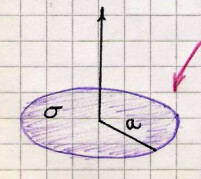
\includegraphics[width=0.25\textwidth]{images/fig_ft1_disco_cargado.jpg}	 


\end{ejemplo}

\begin{ejemplo}{\bf Aros cargados}


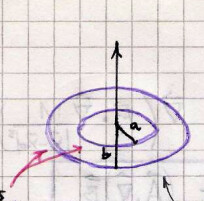
\includegraphics[width=0.25\textwidth]{images/fig_ft1_aros_cargados.jpg}

En este caso la carga total es nula, el monopolo es nulo entonces.
\[
	\lambda_A = \frac{Q}{2 \pi a } \qquad \lambda_B = \frac{Q}{2 \pi b }
\]
de manera que 
\[
	|\lambda_A| = | \lambda_B | \: \frac{b}{a}
\]
El dipolo será nulo respecto del origen y respecto a otros puntos también.
El tensor cuadripolar está caracterizado por un sólo número (luego consideramos a los átomos neutros
monopolar y dipolarmente) $ Q_n = e^{-1} Q_{zz}$.
\notamargen{Algunos momentos cuadripolares nucleares:
Para el $^{14}\mathrm{N}$ es $Q= 7.1\cdot 10^{-2}$ y para el $^{35}\mathrm{Cl}$ es $Q= -7.9\cdot 10^{-2}$}
\end{ejemplo}

\subsection{Momento cuadripolar de un elipsoide}

\[
	\frac{x^2}{A^2} + \frac{y^2}{B^2} + \frac{z^2}{C^2} = 1
\]
y la componente $Q_{11}$ del tensor (que es de traza nula) es
\[
	Q_{xx} = \int \rho( \vbx ) ( 3x^2 - r^2 ) \: d^3x = \rho \int ( 2 x^2 - y^2 - z^2 ) d^3x
\]
donde el tercer término es porque consideramos densidad constante (un elipsoide uniformemente cargado).
Para integrar se hace un cambio de coordenadas
\[
	x'= \frac{x}{A}; \quad y'= \frac{y}{B}; \quad z'= \frac{z}{C};
\]
y entonces se tienen
\[
	Q_{xx} = \frac{q}{5}(2A^2-B^2-C^2) \qquad 
	Q_{yy} = \frac{q}{5}(2B^2-C^2-A^2)  \qquad 
	Q_{zz} = \frac{q}{5}(2C^2-A^2-B^2)
\]
siendo q la carga total. Si el eje $z$ es el de revolución, entonces $A=B$ y se dan
\[
	Q_{xx} = Q_{yy} = \frac{q}{5}(A^2-C^2) \qquad \qquad Q_{zz} = \frac{2q}{5}(C^2-A^2)
\]

\notamargen{Observaciones marginales:
$C_{ij}$ tiene más términos de los que necesito para describir un potencial.
$Q_{ij} = C_{ij}-$ traza, usamos tensor de traza nula.}

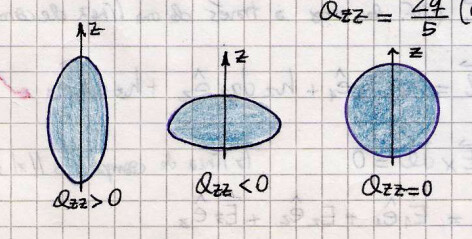
\includegraphics[width=0.4\textwidth]{images/fig_ft1_3elipsoides.jpg}	


\subsection{Interacción de un campo externo con una distribución de carga}

Si tenemos un campo \vb{E} con sus fuentes lejos,


% \begin{figure}[!h]
% 	\begin{center}
	\includegraphics[width=0.4\textwidth]{images/fig_ft1_dipolar3.pdf}	 
% 	\end{center}
% 	\caption{}
% \end{figure}


y que cumple $\divem{E}=0$ y $\rotorm{E}=0$ (irrotacionalidad), se da la siguiente fuerza sobre la distribución
\[
	\vb{F} = \int_V \rho(\vb{x}) \: \vb{E}(\vb{x}) \: dV,
\]
y si \vb{E} no varía demasiado en $V$, entonces podemos representar bien por una serie
\[
	E^\ell(\vb{x}) = E^\ell + x_j \partial_j E^\ell + \frac{1}{2} x_j x_k \partial_j\partial_k E^\ell
\]
entonces 
\[
	F_i = \int_V \rho E_i dV \approx E_i \int_V \rho dV + \int_V \rho  x_j \partial_j E_i dV +
		\frac{1}{2} \int_V \rho x_j x_k \partial_j\partial_k E_i dV 
\]
\notamargen{En la carpeta puse que la integral del cuadrupolo da: $Q_{kj} \partial_k \partial_j E_i$.}
o bien 
\[
	F_i = \int_V \rho E_i dV \approx E_i q + (\vb{p}\cdot\Nabla) E_i  +
		\vb{x}\cdot\left[ (\vb{x}\cdot\Nabla)\Nabla E_i\right]
\]
de lo cual extraemos que el campo interactúa con la carga, el gradiente del campo interactúa con el dipolo
y la divergencia del campo interactúa con el cuadrupolo.
Un campo uniforme entonces no hace fuerza sobre un dipolo.
Para un campo inhomogéneo, el torque $\vb{\Tau} = \vb{x} \times \vb{F}$ se puede escribir como 
\[
	\vb{\Tau} = q\vb{x} \times \vb{E} = \vb{p} \times \vb{E}
\]
donde $\vb{p}\equiv q\vb{x}$ es el momento dipolar y vemos que el torque tiende a centrar el dipolo
según la dirección del campo \vb{E} aunque no lo logra por la agitación térmica.

En la carpeta escribí que reescribía un término de la expansión como
\[
	\frac{1}{2} x_j x_k \partial_j\partial_k E_i =
	\frac{1}{2} \left[ x_j x_k \partial_j\partial_k E_i - \frac{1}{3} r^2 \delta_{ik} \partial_j \partial_k E_i
	\right]
\]
calculo que para lograr que seaa el cuadrupolo la integral. Es la componente sub-$i$ del Laplaciano.


La energía de un dipolo será
\[
	U = -\vb{p}\cdot\vb{E}
\]
entonces
\[
	\vb{F} = -\Nabla U = \Nabla(\vb{p}\cdot\vb{E}) = (\vb{p}\cdot\Nabla)\vb{E} + (\vb{E}\cdot\Nabla)\vb{p}
	+ \vb{p}\times(\rotorm{E}) + \vb{E}\times(\Nabla\times\vb{p})
\]
siendo los últimos tres términos nulos según lo que consideramos previamente de manera que
\[
	\vb{F} = (\vb{p}\cdot\Nabla)\vb{E}.
\]

\subsection{Capa dipolar}

El potencial de un dipolo es
\[
	\phi(\vb{x}) = \frac{ \vb{p}\cdot(\vb{x}-\vb{x}_0) }{|\vb{x} - \vb{x}_0|^3} 
\]
y el potencial de una capa dipolar
\[
	\phi(\vb{x}) = \int_S \frac{ \vb{D}(\vb{x}')\cdot(\vb{x}-\vb{x}') }{|\vb{x} - \vb{x}'|^3} \: dS'
\]
siendo $\vb{D}$ el momento dipolar por área que viene de acuerdo a la definición
\[
	D = \lim_{\substack{\sigma\to\infty \\ \epsilon\to 0}} \: \sigma \: \epsilon
\]
refiérase a la ilustración bajo esta línea. Pero antes algunas cuentas con los dedos
\[
	\delta \phi = \frac{ \delta \vb{p}\cdot(\vb{x}-\vb{x}_0) }{|\vb{x} - \vb{x}_0|^3} 
\]
\[
	\delta \vb{p}(\vbx') = \vb{D}(\vbx') \delta S'
\]
\[
	\int_S d \phi(\vb{x}) = 
	\int_{S'} \frac{ \vb{D}(\vb{x}')\cdot(\vb{x}-\vb{x}') }{|\vb{x} - \vb{x}'|^3} \: dS'
\]

% \begin{figure}[htb]
% 	\begin{center}
	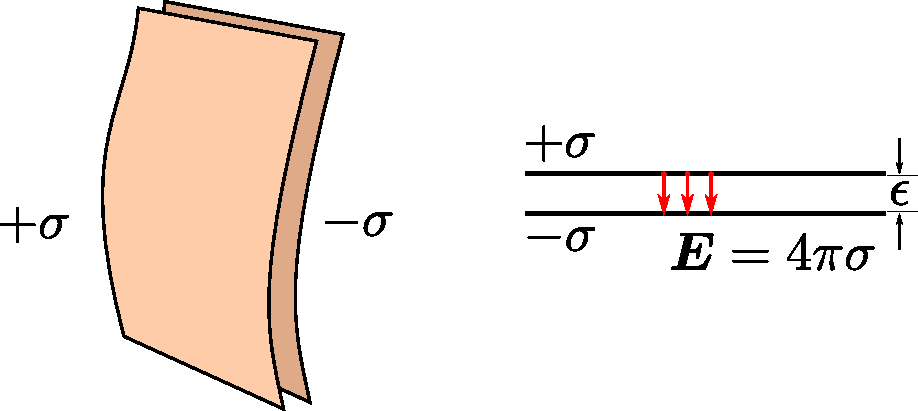
\includegraphics[width=0.75\textwidth]{images/fig_ft1_campo_dipolar3.pdf}	 
% 	\end{center}
% 	\caption{}
% \end{figure}

Veamos algún detalle más sobre la capa dipolar, que está ilustrado en la Figura siguiente.
\[
	\frac{ \vb{D}\cdot(\vb{x}-\vb{x}')}{|\vb{x} - \vb{x}'|^3} dS = 
	\frac{ D \cdot(\vb{x}-\vb{x}')}{|\vb{x} - \vb{x}'|^3} d\vb{S} = 
	- \frac{ D \cos(\theta)}{|\vb{x} - \vb{x}'|^2} dS = 
	- \frac{ D \cos(\theta)}{r^2} dS  
\]

\begin{figure}[htb]
	\begin{center}
	\includegraphics[width=0.6\textwidth]{images/fig_ft1_campo_dipolar1.pdf}	 
	\end{center}
	\caption{}
\end{figure}

\[
	\frac{ \vb{D}\cdot(\vb{x}-\vb{x}')}{|\vb{x} - \vb{x}'|^3} dS = - D d\Omega
\]
puesto que
\[
	\phi(\vb{x}) = -D \int_S d\Omega \qquad \qquad \frac{\cos(\theta)}{r^2}dS \equiv d\Omega
\]

Para las condiciones de contorno se da lo siguiente
\[
	E_2^{\hat{n}} - E_1^{\hat{n}} = 4\pi\sigma
\]
\[
	- \Nabla (\phi_2 - \phi_1)\cdot \hat{n} = 4\pi\sigma
\]
\[
	\dpar{\phi_1 - \phi_2}{\hat{n}} = 4\pi\sigma
\]
\[
	\phi_1 - \phi_2 = 4\pi\sigma\:\epsilon
\]

Y el cálculo del trabajo
\[
	W_{1\to 2} = - q \: 4 \pi \sigma \:\epsilon = q\:( \phi_1 - \phi_2 )
\]
desde donde deducimos que el potencial tiene un salto al surcar la capa dado por 
\[
	\phi_2 - \phi_1 = 4\pi D
\]
Entonces, asociado a una capa dipolar hay un salto de $4\pi D$.

\notamargen{Acá hay que trabajar mejor esto de la capa dipolar en referencia a las BC.
Además saber si lo del $W$ de 1 a 2 es usar la integral de línea por un camino perpendicular
a la surface.}

Para dos chapas infinitas de carga uniforme $\sigma$ pero opuesta el campo eléctrico es nulo 
en todas partes salvo en el interior, donde vale $4\pi\sigma$ (véase ilustración abajo).
Luego el potencial tiene un salto de $4\pi\sigma d$ que se produce a lo largo de la distancia
$d$.

\begin{figure}[htb]
	\begin{center}
	\includegraphics[width=0.4\textwidth]{images/fig_ft1_campo_dipolar2.pdf}	 
	\end{center}
	\caption{}
\end{figure}

Si se considera el límite $\sigma \to \infty$ y $d\to 0$ se tiene una capa dipolar y lo 
que sucede es que la subida apreciable dada por la recta se colapsa a un escalón.


\subsection{Momento dipolar por unidad de volumen}

El potencial de un dipolo es
\[
	\phi(\vb{x}) = \frac{ \vb{p}\cdot(\vb{x}-\vb{x}') }{|\vb{x} - \vb{x}'|^3} 
\]
Suponiendo una distribución continua de dipolos dada por $\vb{P}(\vbx)$, el potencial total debido
a la misma se obtiene de la integración
\[
	\phi(\vb{x}) = \int_V \frac{ \vb{P}(\vb{x}')\cdot(\vb{x}-\vb{x}') }{|\vb{x} - \vb{x}'|^3}  \: dV,
\]
donde $\vb{P}$ es la llamada polarización, el momento dipolar por unidad de volumen, siendo $V$ un volumen
que incluye a la zona de polarización (ver Figura).
\begin{figure}[htb]
	\begin{center}
	\includegraphics[width=0.3\textwidth]{images/fig_ft1_dipolarvol.pdf}	 
	\end{center}
	\caption{}
\end{figure}
Este volumen debe incluir a la misma aunque puede no coincidir con ella.
El potencial se puede escribir como 
\[
	\phi(\vb{x}) = \int_V \vb{P}(\vb{x}')\cdot \Nabla' \left(\frac{1}{|\vb{x} - \vb{x}'|} \right)\: dV
\]
Luego, usando la identidad ID 1 (apéndice) la anterior integral resulta en
\[
	\phi(\vb{x}) = \int_V  \Nabla' \cdot \left( \frac{\vb{P}(\vb{x}')}{|\vb{x} - \vb{x}'|} \right) \: dV
	- \int_V \frac{ \Nabla' \cdot \vb{P}(\vb{x}') }{|\vb{x} - \vb{x}'|} \: dV
\]
y si usamos el teorema de la divergencia en la primera integral se tiene
\[
	\phi(\vb{x}) = \int_S \frac{\vb{P}(\vb{x}')}{ |\vb{x} - \vb{x}'|} \: dS
	- \int_V  \frac{  \Nabla' \cdot \vb{P}(\vb{x}') }{|\vb{x} - \vb{x}'|} \: dV, 
\]
lo que habilita a pensar que el borde del cuerpo polarizado tiene una densidad de carga
de polarización
\[
	\sigma_P = \vb{P}\cdot\hat{n},
\]
y que en el interior existe una carga de polarización volumétrica
\[
	\rho_P = - \Nabla\cdot\vb{P},
\]
siempre y cuando $\divem{P}\neq 0$, es decir que la polarización no sea homogénea.

\begin{ejemplo}{\bf Problema 3}
 
\end{ejemplo}

\begin{ejemplo}{\bf Problema 4}
 
\end{ejemplo}

% =================================================================================================
\section{Desarrollo multipolar para el campo magnético}
% =================================================================================================

Haremos una especie de desarrollo multipolar del potencial vector \vb{A},
\[
	\vb{A}(\vb{x}) = \frac{1}{c} \int_V \frac{\vb{J}(\vb{x}')}{|\vb{x}-\vb{x}'|} \: dV' 
\]
quedándonos a primer orden para $\vbx$ en torno a $\vb{x}'=0$. Es decir, se empleará
\[
	\frac{1}{|\vb{x}-\vb{x}'|} \approx \frac{1}{|\vb{x}|}  + \frac{\vb{x}\cdot\vb{x}'}{|\vb{x}|^3} 
\]
lo cual conduce a
\notamargen{Recordar que Biot \& Savart es para densidad de corriente estacionaria,
i.e. $\divem{J}=0$}
% \[
% 	\vb{A}(\vb{x}) = \frac{1}{c} \int_V \frac{\vb{J}(\vb{x}')}{|\vb{x}|} \: dV' 
% 	+ \frac{1}{c} \frac{ \vb{x} \: }{|\vb{x}|^3} \cdot \int_V \vb{x}' \vb{J}(\vb{x}') \: dV' 
% \]
\[
	\vb{A}(\vb{x}) = \frac{1}{c|\vb{x}|} \int_V \vb{J}(\vb{x}') \: dV' 
	+ \frac{1}{c} \frac{ \vb{x} \: }{|\vb{x}|^3} \cdot \int_V \vb{x}' \vb{J}(\vb{x}') \: dV' 
\]
donde el primer término es nulo lo cual se verá a continuación. En notación indicial la integral
que interesa es 
\[
	\int_V J_i (\vb{x}') \: dV',
\]
luego notemos que 
\[
	\partial_k ( J_k x_i ) = ( \partial_k  J_k ) x_i + J_k \partial_k x_i 
\]
donde el primer término es nulo por ser la divergencia de $\divem{J}$ y el segundo es la delta
de Kronecker de tal forma que
\be
	\partial_k ( J_k x_i ) = J_k \delta_{ki} = J_i. 
	\label{expresion_J}
\ee
El teorema de la divergencia entonces nos asegura que
\[
	\int_V \partial_k ( J_k x_i ) \: dV = \int_S J_k x_i \: dS
\]
donde debe notarse que si la superficie es tal que engloba a todas las corrientes $J$ entonces
ya no hay corriente sobre la superficie y el integrando es nulo.

Se quiere ver que vale 
\[
	\int_V J_i \: x_k \: dV = - \int_V J_k \: x_i \: dV,
\]
y para ello veamos qué le pasa a la divergencia de un tensor de tercer rango, que se puede
escribir
\[
	\partial_l( x_i J_l x_k ) =  \partial_l( x_i J_l ) \: x_k + x_i J_l \:\partial_l( x_k )
\]
usando el resultado anterior \eqref{expresion_J} es
\[
	\partial_l( x_i J_l x_k ) = J_i \: x_k + x_i J_k,
\]
y como es
\[
	\int_V (J_i \: x_k + x_i J_k ) \: dV = 0.
\]
\notamargen{Parece que acá termina la cosa. No me queda nada claro.}
% puede verse porque sale integrando con alguna identidad (?)
% y usando que $\divem{J}=0$. 

Por otra parte, dado que 
\[
	\vbx \times ( \vbx'\times \vb{J}) = (\pe{x}{J})\: \vbx'- \vb{J} \: (\pe{x}{x'} )
\]
se puede aplicar esto en la integración del segundo término
\[
	\int_V x_i J_k x_i' \: dV' = \int_V x_i J_i x_k' \: dV' - \int_V \vbx \times ( \vbx' \times \vb{J} )_k \: dV'
\]
donde el primero aquí será nulo porque es idéntico al anterior, y entonces
\[
	\int_V x_i J_k x_i' \: dV' = - \frac{1}{2} \: \vbx \times \int_V  ( \vbx' \times \vb{J} )_k \: dV',
\]
quedando en deuda la explicación del $1/2$.

\notamargen{Esto habrá que hacerlo bien. La notación está muy poco consistente.}

Este término que resultó nulo correspondería al orden monopolar y su nulidad refleja la no existencia 
de monopolos magnéticos.

Esto conduce a 
\[
	\vb{A}(\vb{x}) = \frac{1}{|\vb{x}|^3} 
	\left[ \left(\frac{1}{2c} \int_V \vb{x}'\times \vb{J} \: dV \right) \times \vb{x} \right] 
\]
y si definimos el corchete como \vb{m} (momento magnético) entonces
\[
	\vb{A}(\vb{x}) = \frac{\vb{m} \times \vb{x} }{|\vb{x}|^3}
\]
en el origen, y 
\[
	\vb{A}(\vb{x}) = \frac{\vb{m} \times (\vb{x}-\vb{x}') }{|\vb{x}-\vb{x}'|^3}
\]
desplazado hacia $\vb{x}'$, las cuales son expresiones a primer orden y que utilizan el gauge de Coulomb, 
$\divem{A}=0$.

De esta manera tendremos
\[
	\mathcal{M}(\vb{x}') = \frac{1}{2c} \left[ \vb{x}' \times \vb{J}(\vb{x}')\right]
\]
que es la magnetización o densidad de momento magnético, y entonces el momento magnético pasa a ser 
\[
	\vb{m} = \int_v \mathcal{M}(\vb{x}') \:dV'.
\]

Ahora se querrá ver qué le pasa al rotor de $\vb{A}$. Para ello se usa la identidad vectorial I2 del apéndice.
Considerando $\vb{m} = \vb{M}$ y $\vb{N} = \vbx / |\vbx|^3 $ se tiene 
\[
	\Nabla \times \left( \frac{\vb{m} \times \vb{x} }{|\vb{x}|^3} \right) =
	\vb{m} \: ( \Nabla \cdot \vbx / |\vbx|^3 ) - \vb{N} \: ( \divem{m} ) +
	( \vbx / |\vbx|^3 \cdot \Nabla ) \: \vb{m} - ( \vb{m} \cdot \Nabla ) \: \vbx / |\vbx|^3,
\]
donde los dos primeros términos son nulos \footnote{El segundo es nulo porque $\vb{m}$ no depende de $\vbx$}. 
Entonces
\[
	\rotorm{A} = -( \vb{m} \cdot \Nabla ) \: \frac{\vbx}{|\vbx|^3} + 4 \pi \delta(\vb{x}) \: \vb{m},
\]
pero el segundo término con la delta no se considerará porque estamos lejos de la distribución de
corrientes\footnote{El término con la delta de Dirac cobra importancia en análisis microscópicos y
cuánticos}. Luego,
\[
	\rotorm{A} = \Nabla \times \left( \frac{\vb{m} \times \vb{x} }{|\vb{x}|^3} \right) =
	-(\vb{m}\cdot\Nabla)\frac{\vb{x}}{|\vb{x}|^3}.
\]
Recordando la expresión para el momento dipolar del campo eléctrico (buscarla) como
\[
	\vb{E}^{(2)} = - ( \vb{p}\cdot\Nabla) \frac{\vbx}{|\vbx|^3},
\]
que llevaba a $\vb{E}^{(2)} = ( 3 (\vb{P}\cdot \hat{n}) \hat{n} - \vb{P} )/ |\vbx|^3$, por analogía
se tendrá
\[
	\vb{B} = \frac{3 (\vb{m}\cdot\hat{n})\hat{n} - \vb{m}}{|\vb{x}|^3},
\]
que nos dice que bien lejos cualquier distribución de corriente localizada \vb{B} se presenta como el 
campo magnético de un dipolo magnético dado por \vb{m}(\vb{x}). Esta aproximación corresponde, por 
supuesto, al primer orden del desarrollo.
El momento magnético puede pensarse entonces como una espirilla.

\subsection{Interpretacion del momento magnético}

Se puede pensar al \vb{m} como una espira plana, lo cual nos provee de una noción intuitiva del 
momento dipolar magnético. 
Entre un punto $\vbx$ del borde y un diferencial de arco $d\Bell$ queda definido un triángulo infinitesimal
cuya área $dA$ será 
\[
	dA = \frac{ 1 }{ 2 } x \: \sin(\alpha) \: d\ell, 
\]
que no es otra cosa que el área de un triángulo (base por altura sobre dos), siendo el área orientada
\[
	\vb{A} = \frac{1}{2} \int_\Gamma \vb{x}\times d\Bell  
\]
y entonces
\[
	\vb{m} = \frac{I}{c}\vb{A}
\]
\begin{figure}[htb]
	\begin{center}
	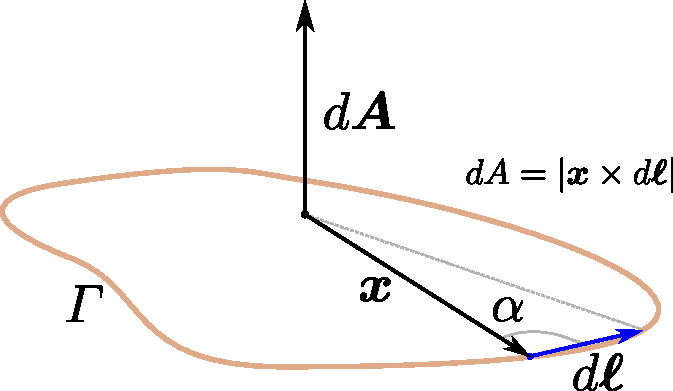
\includegraphics[width=0.5\textwidth]{images/fig_ft1_mmag.pdf}	 
	\end{center}
	\caption{}
\end{figure}

Para convertir un volumen a espira hacemos la transformación del modo usual,
\[
	\vb{m} = \frac{1}{2c} \int_V  \vb{x} \times \vb{J}(\vb{x})  \:dV =
		\frac{I}{2c} \int_\Gamma  \vb{x} \times \:d\Bell
\]
usando que
\[
	\vb{J} \: dV = J \: d\Bell \: dS = \frac{I}{dS} \: d\Bell \: dS = I \: d\Bell 
\]

A modo de ejemplo, para una espira circular de radio $r$ es
\[
	m = \frac{i}{c} \pi r^2.
\]

\subsection{Interacción del campo magnético con una distribución de corriente}

La idea es considerar la fuerza sobre una distribución de corrientes debida a un campo
externo homogéneo.
Hacemos una expansión de Taylor del campo \vb{B} con $|\vb{x}|\ggg|\vb{x}'|$,
\[
	\vb{B} = \vb{B}_0 + (\vb{x}\cdot\Nabla)\vb{B}
\]
y entonces como la fuerza es
\[
	\vb{F} = \frac{1}{c} \int_V \vb{J}(\vb{x}') \times \vb{B}(\vb{x}') \: dV'
\]
\begin{figure}[htb]
	\begin{center}
	\includegraphics[width=0.5\textwidth]{images/fig_ft1_campocorr.pdf}	 
	\end{center}
	\caption{}
\end{figure}
resulta que
\[
	\vb{F} =  \frac{1}{c} \int_V \vb{J} \times \vb{B}_0 \: dV' +
		\frac{1}{c} \int_V \vb{J} \times (\vb{x}'\cdot\Nabla)\vb{B} \: dV'
\]
siendo el primer término nulo.

Mediante identidades vectoriales podemos llegar a una expresión
\[
	\vb{F} = - \Nabla \times \frac{1}{c} \int_V \vb{J}(\vb{x}'\cdot\vb{B}) dV'
\]
y utilizando la demostración previa de que 
\[
	\int \: (\vbx \cdot \vbx') \: \vb{J} \: dV = 
	- \frac{1}{2} \: \vbx \times \int \: \vbx \times \vb{J} \: dV,
\]
resulta que 
\[
	\vb{F} = \Nabla \times \vb{B} \times \frac{1}{2c} \int_V \vb{x} \times \vb{J} \: dV
\]
y entonces, identidades vectoriales mediante,
\[
	\vb{F} = \Nabla\times(\pv{B}{m}) = (\pe{m}{\Nabla})\vb{B} = \Nabla(\pe{m}{B})
\]
Si el campo es homogéneo la fuerza es nula.
Por otra parte, como $\vb{F} = -\Nabla U$ se puede definir energías para los dipolos
de acuerdo con el esquema
\[
	F_m = \Nabla(\pe{m}{B}) \quad \Rightarrow \quad U_m = -\pe{m}{B}
\]
\[
	F_e = \Nabla(\pe{p}{E}) \quad \Rightarrow \quad U_e = -\pe{p}{E}
\]
siendo $U_{m,e}$ la energía de los dipolos en campos externos.

La fuerza de un campo $\vb{B}$ externo sobre una distribución de corrientes es el gradiente de cierta
energía
\[
	\vb{F} = \Nabla(\vb{m}\cdot\vb{B}) = (\vb{m}\cdot\Nabla)\vb{B}
\]
de donde se ve claramente que si \vb{B} es uniforme entonces la fuerza es nula.
\vb{m} es una constante que depende de la distribución de corrientes.

\begin{ejemplo}{\bf Problema 6b}

Ahora $ a \ll L $ y por la simetría de rotación son convenientes coordenadas cilíndricas.
La simetría reclama que no hay dependencia en $ \vp $ ni componente $B_\vp$ de manera que
\[
	\vb{B}(r,z) = B_z(r,z) \zver + B_r(r,z) \rver
\]
Considerando una expansión de Taylor para $r$ pequeños
\[
	B_z(r,z) \approx B_z(0,z) + \left.\dpar{B_z}{r}\right|_{r=0} r\qquad \qquad 
	B_r(r,z) \approx B_r(0,z) + \left.\dpar{B_r}{r}\right|_{r=0} r
\]

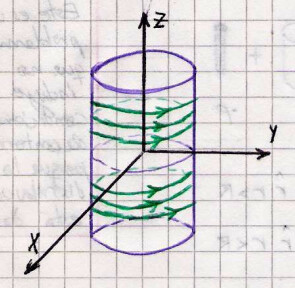
\includegraphics[width=0.4\textwidth]{images/fig_ft1_problema_6b.jpg}

La simetría dice también que  $B_r(0,z) = 0$ y utilizando la divergencia nula $\divem{B}=0$ del campo en
cilíndricas se tiene 
\[
	\frac{1}{r} \dpar{rB_r}{r} + \dpar{B_z}{z} = 0,
\]
o bien
\[
	\dpar{B_r}{r} = - \dpar{B_z}{r} - \left.\dpar{B_z}{r}\right|_{r=0}
\]
y evaluando en $r=0$ se obtiene [CHECK ESTO]
\[
	\left. \dpar{B_r}{r} \right|_{r=0} = 
	- \frac{1}{2} \left. \dpar{B_z}{r} \right|_{r=0}
\]
Se obtiene una expresión algo más general que la que se hubo obtenido (la de la clase pasada, que es la
del capítulo 1)  que utilizaba $ L \to \infty $.
 
\end{ejemplo}

\begin{ejemplo}{\bf Problema 11}

Este es un problema que no incluye condiciones de contorno porque la distribución de carga está dada.
Es un cilindro infinito.
Si hacemos el potencial $\vp$ aquí vemos que revienta lo cual se debe a que la distribución de carga
es infinita.

El arreglo es el de la figura

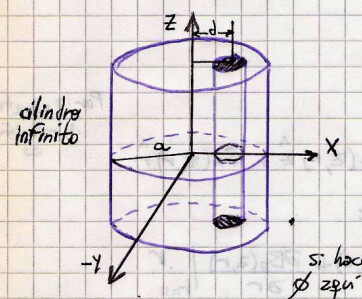
\includegraphics[width=0.375\textwidth]{images/fig_ft1_problema_11a.jpg}

También se puede pensar de la siguiente forma

\includegraphics[width=0.5\textwidth]{images/fig_ft1_problema_11b.jpg}

El campo para un cilindro de radio $R$ centrado en $r=0$ es 
\[
	\vb{E}  = 
	\begin{cases} 
		\displaystyle \frac{2 \pi a^2 \rho }{r} \rver & \qquad r \geq R  \\
		\\
		2 \pi r \rho \rver & \qquad r < R
	\end{cases}
\]
Escribiendo el campo interno como 
\[
	2 \pi r \rho \rver = 2 \pi \rho \: \vb{x},
\]
donde $\vbx = r \rver $ es el vector que vive en el plano horizontal, se puede trasladar el cilindro
así 
\[
	2 \pi \rho ( \vb{x} + d \xver )
\]
y entonces el campo dentro del cilindro es
\[
	\vb{E} = 2 \pi \rho d \xver.
\]

\notamargen{Hay que mirar la práctica porque esto está confuso.}

Para la parte (b) se considera

\includegraphics[width=0.2\textwidth]{images/fig_ft1_problema_11c.jpg}

\includegraphics[width=0.3\textwidth]{images/fig_ft1_problema_11d.jpg}

\[
	B(r) 2 \pi r = \frac{4\pi}{c} \pi r^2 j,
\]
pero $\vb{B}$ es en $\phiver$ y entonces
\[
	\vb{B} = \frac{2\pi r j}{c} \frac{\phiver}{r} = \frac{2\pi j}{c} ( -y \xver + x \yver )
\]
de manera que el campo total, que es la suma de los campos del cilindro grande
y del pequeño, será
\[
	\vb{B} = \frac{2\pi j}{c}( -y \xver + d\yver + x \yver ) - \frac{2\pi j}{c}( -y \xver + x \yver ),
\]
o bien
\[
	\vb{B} = \frac{2\pi j}{c} d \yver.
\]
 
\end{ejemplo}

\begin{ejemplo}{\bf Problema 13}

Esfera central a tierra, esfera externa con densidad superficial $\sigma$.
La siguiente equivalencia es posible

\includegraphics[width=0.5\textwidth]{images/fig_ft1_problema_13a.jpg}

Luego, esto se resuelve así, usando la simetría esférica y la ley de Gauss $ \int \vb{E}\cdot d\vb{S} = 4 \pi Q$
se tienen
\[
	4 \pi r^2 E = \begin{cases} 
	               0 \\
	               4 \pi a^2 \sigma
	              \end{cases}
	\qquad 
	4 \pi r^2 E = \begin{cases} 
	               0 \\
	               4 \pi b^2 \sigma'
	              \end{cases} 
\]
\[
	\vb{E} = \begin{cases}
	          \displaystyle 4 \pi \frac{\sigma a^2 + \sigma' b^2 }{r^2} \rver \quad & r > b \\ 
	          \\
	          \displaystyle 4 \pi \frac{\sigma' b^2}{r^2} \rver \quad & a < r < b \\
	          \\
	          0 & r < a 
	         \end{cases}
\]
El potencial será
\[
	V = \begin{cases}
	          \displaystyle 4 \pi \frac{\sigma a^2 + \sigma' b^2 }{r} + C_1 \quad & r > b \\ 
	          \\
	          \displaystyle 4 \pi \frac{\sigma' b^2}{r}  + C_2 \quad & a < r < b \\
	          \\
	          C_3 & r < a 
	         \end{cases}
\]
y al pedir continuidad para el mismo, se tienen 
\[
	C_1 = 0, \qquad C_2 = 4 \pi \sigma, \qquad C_3 = 0 
\]
donde en la última está metida la $\sigma'$ que hace nulo el potencial $V$ sobre la esfera
interna. Así, finalmente
\[
	V = \begin{cases}
	          \displaystyle 4 \pi \frac{\sigma a (a-b)}{r} \quad & r > b \\ 
	          \\
	          \displaystyle 4 \pi \frac{\sigma a (r-b)}{r} \quad & a < r < b \\
	          \\
	          0 & r < a 
	         \end{cases}
\]

Una serie de diagramitas a descular siguen:

\includegraphics[width=0.5\textwidth]{images/fig_ft1_problema_13b.jpg}
 
\end{ejemplo}



% =================================================================================================
\section{Perturbación por un conductor sobre un campo eléctrico uniforme}
% =================================================================================================

Se tiene un campo uniforme con $Q,R \to \infty$ pero con $2Q/R^2 = cte$, según se ve en la Figura.


El potencial $\phi$ de la esfera es constante por ser conductor.
Puedo definir 
\[
	\phi|_{esf} \equiv 0
\]
pues $\phi(\infty)\neq 0 $ porque hay densidad de carga $\rho$ en el infinito.

\begin{figure}[htb]
	\begin{center}
	\includegraphics[width=0.4\textwidth]{images/fig_ft1_perturbacion1.pdf}	 
	\end{center}
	\caption{}
\end{figure}
Para la carga superior,
\[
	\phi_1 = \frac{-Q}{|\vb{x} - R\hat{z}|} + \frac{a/R Q}{|\vb{x} - a^2/R\hat{z}|}
\]
mientras que para la inferior
\[
	\phi_2 = \frac{Q}{|\vb{x} + R\hat{z}|} + \frac{ a/R Q}{|\vb{x} + a^2/R\hat{z}|}
\]

Recordemos que
\[
	(1+\alpha)^{(-1/2)} \approx 1 - \frac{1}{2}\alpha \qquad \alpha \ll 1
\]
y podemos trabajar el denominador
\[
	|\vb{x} - R\hat{z}| = \sqrt{ x^2 + R^2 - 2Rx\cos(\theta)}
\]
\[
	\frac{1}{|\vb{x} - R\hat{z}|} = \frac{1}{\sqrt{ x^2 + R^2 - 2Rx\cos(\theta)}} =
	\frac{1}{R(1 + x^2/R^2 - 2x/R\cos(\theta))^(1/2)}
\]
\[
	\frac{1}{|\vb{x} - R\hat{z}|} \approx \frac{1}{R}\left(1+ \frac{x}{R} \cos(\theta) \right)
\]
de manera que luego
\begin{multline*}
	\phi(r) \approx Q\left[ \frac{1}{R}\left(1+ \frac{x}{R} \cos(\theta) \right) + 
	\frac{a}{Rx}\left(1+ \frac{a^2}{Rx} \cos(\theta) \right) + \right. \\
	\left. \frac{1}{R}\left(1 - \frac{x}{R} \cos(\theta) \right) -
	\frac{a}{Rx}\left(1 - \frac{a^2}{Rx} \cos(\theta) \right) \right]
\end{multline*}
\[
	\phi(x) \approx -\frac{2Qx}{R^2} \cos(\theta) + \frac{2a^3Q}{R^2x^2}\cos(\theta)
\]
y haciendo $x\equiv r$ y tomando el límite,
\[
	\phi(r) = -E_0 r \cos(\theta) + E_0\frac{a^3}{r^2} \cos(\theta)
\]
y la carga total sobre la esfera es nula puesto que estuvo aislada todo el tiempo.
Respecto de la Figura, si hacemos un Gauss en la zona indicada se obtiene $Q_n=0$,
entonces $\phi(r=a)=0$.

\begin{figure}[htb]
	\begin{center}
	\includegraphics[width=0.2\textwidth]{images/fig_ft1_perturbacion3.pdf}	 
	\end{center}
	\caption{}
\end{figure}

El segundo término es como un dipolo puntual,
\[
	E_0\frac{a^3}{r^2} \cos(\theta) = E_0\frac{a^3 \hat{z}\cdot\vb{r}}{r^3} 
\]
donde
\[
	\vb{p} \equiv E_0 a^3 \hat{z}
\]



\begin{notasfinales}

\label{notas_carga_frente_a_esfera}
\item{ \bf Sobre el problema de la carga frente a la esfera conductora a tierra}

Decíamos que esta solución se puede obtener de manera más heurística, como lo hace Jackson? [CITA],
a partir de la expresión en 
\[
	\frac{q}{\sqrt{ a^2 + y^2 - 2 \: a \: y \:\cos{\gamma}} } +
	\frac{q'}{\sqrt{ a^2 + y'^2 - 2 \: a \: y' \: \cos{\gamma} }} = 0,
\]
se podría intentar forzar que el segundo denominador sea idéntico al primero para lo cual se puede multiplicar
arriba y abajo por el factor $(y/a) $
\[
	\frac{q}{\sqrt{ a^2 + y^2 - 2 \: a \: y \:\cos{\gamma}} } +
	\frac{q' (y/a) }{ y/a \sqrt{ a^2 + y'^2 - 2 \: a \: y' \: \cos{\gamma} }} = 0
\]
lo que conduce a
\[
	\frac{q}{\sqrt{ a^2 + y^2 - 2 \: a \: y \:\cos{\gamma}} } +
	\frac{q' (y/a) }{\sqrt{ y^2 + y^2y'^2/a^2 - 2 \: y^2/a \: y' \: \cos{\gamma} }} = 0
\]
y esta ecuación se satisface si $ y y'= a^2 $ y si $ q = - q' (y/a)$, que es justamente la solución
encontrada previamente de un modo más tradicional.

También es interesante considerar algunos casos límite y ver que se recuperan resultados y comportamientos
familiares. Si $ q $ está localizada muy cerca de la superficie de la esfera, i.e. $ |\vb{y}| \approx a + \varepsilon $
resultan $ y' \approx a - \varepsilon $ y $ q' \approx -q + ( \varepsilon / a ) q $ que son exactamente los
resultados para una carga frente a un plano conductor (si despreciamos la cantidad infinitesimal $( \varepsilon / a )$).
Muy cerca de la superficie de la esfera la carga {\it ve} un plano infinito.


\end{notasfinales}


% \bibliographystyle{CBFT-apa-good}	% (uses file "apa-good.bst")
% \bibliography{CBFT.Referencias} % La base de datos bibliográfica

\end{document}

	
		\documentclass[10pt,oneside]{CBFT_book}
	% Algunos paquetes
	\usepackage{amssymb}
	\usepackage{amsmath}
	\usepackage{graphicx}
% 	\usepackage{libertine}
% 	\usepackage[bold-style=TeX]{unicode-math}
	\usepackage{lipsum}

	\usepackage{natbib}
	\setcitestyle{square}

	\usepackage{polyglossia}
	\setdefaultlanguage{spanish}


	\usepackage{CBFT.estilo} % Cargo la hoja de estilo

	% Tipografías
	% \setromanfont[Mapping=tex-text]{Linux Libertine O}
	% \setsansfont[Mapping=tex-text]{DejaVu Sans}
	% \setmonofont[Mapping=tex-text]{DejaVu Sans Mono}

	%===================================================================
	%	DOCUMENTO PROPIAMENTE DICHO
	%===================================================================

\begin{document}

% =================================================================================================
\chapter{Método de separación de variables}
% =================================================================================================

Al resolver una PDE (partial differential equation) se termina en general en un problema de
Sturm-Liouville, que lleva a autovalores y autofunciones.

Un problema regular de Sturm-Liouville está representado por una ecuación del tipo
\[
	\dtot{}{x}\left[ r(x) \dtot{f}{x} \right] + [ q(x) + \lambda p(x)] f = 0,
\]
donde $p(x)$ es una función peso que definenla ortogonalidad (muchas veces vale 1).
Las condiciones de contorno en el intervalo $(a,b)$ serán
\[	
	f(a) + \dtot{f}{x}(a) = \qquad \qquad f(b) + \dtot{f}{x}(b) =
\]

En el (a,b) las condiciones de ortogonalidad se leen
\[
	\int_a^b \: U_n^*(\xi) U_m(\xi) p(\xi) d\xi = 0 \qquad n \neq m
\]
Asimismo, si están normalizadas, se puede escribir
\[
	\int_a^b \: U_n^*(\xi) U_m(\xi) p(\xi) d\xi = \delta_{nm}
\]
Luego, cualquier $f$ (well behaved) en el $(a,b)$ se puede poner como
\[
	f(x) \equiv \sum_{n=1}^N a_n U_n(x)
\]
Entonces
\[
	M_N = \int_a^b \: \left| f(x) - \sum_{n=1}^N \: U_n(x') \right|^2 \: dx,
\]
y esta expresión es mínima cuando los $a_n$ son
\[
	a_n = \int_a^b \: U_n^*(x') \: f(x') \: p(x') \: dx'
\]

Entonces,
\[
	f(x) = \sum_{n=1}^\infty \: U_n(x')
\]
es correcto porque la serie converge. Luego, integrando en $x'$
\[
	f(x) = \int_a^b \left[ \sum_{n=1}^\infty \: U_n^*(x') \: f(x') \: p(x') \: dx' \right] U_n(x)
\]
y donde
\[
	f(x) = \int_a^b \left[ \sum_{n=1}^\infty \: U_n^*(x') U_n(x) \right] \: f(x') \: p(x') \: dx'
\]
es claro que esto debe tener comportamiento de delta de Dirac, y
\[
	\sum_{n=1}^\infty \: U_n^*(x') U_n(x) = \delta(\vbx-\vbx')
\]
es la llamada condición de clausura.

% =================================================================================================
\section{Separación en coordenadas cartesianas}
% =================================================================================================

Separamos los problemas en regiones donde vale $\lapm{\phi} = 0$ entonces las fronteras tendrán la
$\rho(\vb{x}')$ en general en forma de $\sigma,\lambda$.

Para coordenadas cartesianas la ecuación de Laplace $\lapm{\phi} = 0$, adquiere la forma
\[
	\dpar[2]{\phi}{x} + \dpar[2]{\phi}{y}  + \dpar[2]{\phi}{z}  = 0,
\]
que intentaremos resolver a partir de un {\it ansatz} 
\[
	\phi(x,y,z) = X(x) \: Y(y) \: Z(z)
\]
lo que conduce a 
\[
	\frac{1}{X}\dtot[2]{X}{x} + \frac{1}{Y}\dtot[2]{Y}{y} + \frac{1}{Z}\dtot[2]{Z}{z} = 0.
\]
Para que esta solución valga, cada término tiene que ser una constante, entonces primeramente
\[
	\frac{1}{X} \dtot[2]{X}{x} = - \alpha^2
\]
lleva a 
\[
	\frac{1}{Y}\dtot[2]{Y}{y} + \frac{1}{Z}\dtot[2]{Z}{z} = \alpha^2,
\]
y 
\[
	\frac{1}{Y} \dtot[2]{Y}{y} = - \beta^2,
\]
conduce a
\[
	\frac{1}{Z}\dtot[2]{Z}{z} = \alpha^2 + \beta^2 = \gamma^2
\]
donde cada una de estas ecuaciones es una versión simplificada de Sturm-Liouville. En estos
casos particulares son osciladores armónicos; uno en cada dirección.
Luego suponiendo $\alpha,\beta \int \mathbb{R}>0$ será $\gamma \in \mathbb{R}$ y la solución 
general es
\[
	\phi(x,y,z) = \sum_{m=0}^\infty \sum_{n=0}^\infty A_{m,n} \euler^{\pm i\alpha_m x}
	\euler^{\pm i\beta_n y} \euler^{\pm i\sqrt{\alpha_m^2 + \beta_n^2 }z}.
\]
donde $A_{m,n}$ es una constante general. 
Las condiciones de contorno permitirán fijar las constantes y entonces la solución tendrá
diversas formas. 

Según la conveniencia del problema particular será
\[
	\euler^{\pm \gamma x_i } = \cosh( \gamma x_i ) + \sinh( \gamma x_i )
\]
\[
	\euler^{\pm i k x_i } = \cos( k x_i ) + i \sin( k x_i )
\]

\subsubsection{Algunos tips}

Queremos resolver la ecuación de Poisson, 
en el caso de cargas tipo (puntuales, lineales y superficiales)

\includegraphics[width=0.4\textwidth]{images/fig_ft1_tips_separacion.jpg}

podemos resolver $\nabla^2 \vp = 0$ que es más sencilla y separamos en dos
regiones \textcircled{I} y \textcircled{II} donde me preocupo solamente
por Laplace.
Si las fuentes son más complejas que esto nos remitiremos a la función
de Green.

\begin{ejemplo}{\bf Potencial en una caja}

En este caso interesa el potencial $V$ dentro de la caja. El exterior está fuera del ámbito
de la resolución.

\includegraphics[width=0.4\textwidth]{images/fig_ft1_potencial_caja.jpg}

Se plantea para el potencial 
\begin{multline*}
	\phi(x,y,z) =  \sum_{\alpha,\beta} \:
	\left[ A_\alpha\sin( \alpha x) + B_\alpha\cos( \alpha x) \right]
	\left[ C_\beta\sin( \beta y) + D_\beta\cos( \beta y) \right]\times \\
	\left[ E_\gamma\sinh( \gamma z) + F_\gamma\cosh( \gamma z) \right]
\end{multline*}
Utilizando que el potencial es nulo en los contornos indicados (ver figura) resulta
\[
	\phi(0,0,0) = 0 \qquad \longrightarrow \qquad F_\gamma = 0
\]
\[
	B_\alpha = 0 \qquad D_\beta = 0
\]
\notamargen{Tal vez poner que esto es por las tapas laterales.}

Entonces, juntando todas las constantes en una única constante $A$ el potencial será la 
suma siguiente
\[
	\phi(x,y,z) =  \sum_{\alpha,\beta} \:
	A_{\alpha\beta} \: \sin( \alpha x) \: \sin( \beta y) \: \sinh( \gamma z)
\]
donde dada la relación $\gamma^2 = \alpha^2 + \beta^2$ este índice se ha absorbido junto a los
otros dos de manera que solo es una doble sumatoria.

Para satisfacer las condiciones de potencial nulo en $x=a$ y en $y=b$ se deben cumplir
\[
	\alpha = n \frac{\pi}{a} \qquad \beta = m \frac{\pi}{b}
\]
para todo natural $n, m$. Luego
\[
	\gamma = \pi \sqrt{ \frac{n^2}{a^2} + \frac{m^2}{b^2} }.
\]
Entonces, cambiando los índices de la sumatoria a
\[
	\phi(x,y,z) =  \sum_{n,m} \:
	A_{nm} \: \sin\left( n \frac{\pi}{a} x \right) \: \sin\left( m \frac{\pi}{b} y \right)
	\: \sinh\left( \pi \sqrt{ \frac{n^2}{a^2} + \frac{m^2}{b^2} } z \right)
\]

Finalmente sobre la tapa superior será $\phi(x,y,c) = V(x,y)$ de manera que, mediante un
cálculo rutinario llegamos a
\[
	A_{nm} = \frac{4}{ a b \sinh( \pi \sqrt{ n^2/a^2 + m^2/b^2} c )} \:
	\int_0^a \int_0^b \: V( x,y) \: \sin\left( n \frac{\pi}{a} x \right) \: 
	\sin\left( m \frac{\pi}{b} y \right) \: dy dx.
\]

\end{ejemplo}

\begin{ejemplo}{\bf Problema 2}

El problema a resolver está en el sketch de abajo

\includegraphics[width=0.4\textwidth]{images/fig_ft1_problema2_sep_A.jpg}

Queremos que no haya carga en las regiones en las cuales se subdividiráel
espacio nos ocuparemos del laplaciano.

El sistema coordenado a utilizar está mostrado abajo

\includegraphics[width=0.4\textwidth]{images/fig_ft1_problema2_sep_B.jpg}

La densidad de carga se puede escribir según
\[
	\rho(\vbx) = \lambda \delta(x) \delta(z) = \sigma \delta(z)
\]
donde hemos definido una densidad $\sigma$.
La solución será de la forma
\[
	\Phi = X \: Y \: Z,
\]
donde $Y$ será una constante porque el problema no depende de $y$.
Como las funciones trigonométricas se anulan en puntos y $Z$ necesita
esto se eligen
\[
	Z \propto \cos( k_z z ), \sin( k_z z )
\]
y $X \propto \euler^{- K x} $ porque el potencial podría ir decreciendo
en $x$ --aunque es infinito--.
Donde $K=k_z$ y $k_y=0$. Hay una simetría en $xy$ de reflexión, entonces el
potencial es par. Luego, para la base de funciones usaré funciones pares
(cosenos).
Luego,
\[
	\phi(z=\pm a/2) = 0,
\]
por ser planos conductores a tierra. Entonces hacer que se cumpla
\[
	\cos(\pm a/2 K) = 0,
\]
necesita $k_n = ( 2n + 1 ) \pi / a$ (nos alcanza con $\mathbb{N}$ más el cero).
La base de funciones será
\[
	\phi_I = \sum \: A_n^I \: \euler^{-K_n x} \: \cos(K_n z) \qquad 
	x > 0
\]
\[
	\phi_{II} = \sum \: A_n^{II} \: \euler^{K_n x} \: \cos(K_n z) \qquad 
	x < 0
\]

Ahora pediremos condiciones en la superficie de seperación, la continuidad
del potencial
\[
	\phi_I( x=0 ) = \phi_{II}( x=0 )
\]
Entonces, para el campo resultan
\[
	\sum_n^\infty A_n^{I} \cos(k_nz) = 
	\sum_n^\infty A_n^{II} \cos(k_nz)
\]
es decir $A_n^{I}= A_n^{II} \equiv A$, y para las derivadas del potencial
\[
	- \dpar{\phi_I}{x} - \left( - \dpar{\phi_{II}}{x} \right) = 
	4 \pi \lambda \delta(z) |_{x=0}
\]
\[
	2 \sum_n \: k_n A_n \cos( k_n z ) = 4 \pi \lambda \delta(z)
\]

Para despejar el coeficiente se utilizan las propiedades de ortogonalidad,
tomando el producto escalar en ambos miembros de la anterior ecuación,
\notamargen{El período es $a$ pues hay nodos en $\pm a/2$. Se multiplica 
por coseno y se integra.}
\[
	a k_m A_m = 4 \pi \lambda \int_{-a/2}^{a/2} \cos( k_m z ) \delta{z} dz
\]
y como la integral da uno,
\[
	A_n = \frac{ 4 \lambda }{ 2 n + 1 }
\]

Ahora considero el plano $xy$.

\includegraphics[width=0.4\textwidth]{images/fig_ft1_problema2_sep_C.jpg}

Se propone una fórmula 
\[
	\phi = X Y Z,
\]
donde $X$ es una $\euler^{ikx}$, $Y$ es una constante y para $Z$
se toma $ \sinh( k |z - a/2| ) $ porque un solo cero es necesario.
Entonces tenemos prescripciones para cada zona que son 
\[
	\phi_I = \int_{-\infty}^{\infty} \: 
	\sinh( k|z-a/2| ) \: A_k^I \: \euler^{ikx} \: dk
\]
\[
	\phi_{II} = \int_{-\infty}^{\infty} \: 
	\sinh( k|z-a/2| ) \: A_k^{II} \: \euler^{ikx} \: dk
\]

Entonces, de la evaluación de los contornos 
\[
	\phi_I(z=0) = \phi_{II}(z=0)
\]
surgen
\[
	A_k^{I} = A_k^{II} \equiv A_k
\]
y asimismo
\[
	- 2 \int A_k \euler^{ikx} k \cosh( ka/2 ) \: dk 
	- 2 \int A_k \euler^{ikx} k \cosh( ka/2 ) \: dk = 4 \pi \lambda \delta(x)
\]
lo cual nos lleva a
\[
	- 2 \int A_k \euler^{ikx} k \cosh( ka/2 ) \: dk
	= 4 \pi \lambda \delta(x),
\]
y multiplico por $\int \euler{-ik'x} dx$
\notamargen{
Usaremos la expresión de la delta en Fourier:
\[
	2 \pi \delta(k-k') = \int \: \euler^{ i (k - k') x} \: dx
\]}
lo cual lleva a 
\[
	A_k = \frac{-\lambda}{k'\cosh(ka/2)},
\]
y volviendo todo a $k$ sin primar
\[
	\phi = -\lambda \int dk \: \euler^{ikx} \:
	\frac{\sinh( k|z-a/2|)}{k'\cosh(ka/2)}
\]

Para este caso obtenemos para el potencial una integral, contrariamente
a lo que teníamos para el otro caso donde aparecía una serie.

Queremos ver la relación entre ambas,
\[
	\sinh( k |z-a/2 |) = \sum_{n} A_n \cos(k_n z)
\]
Sacamos de una tabla la forma del $A$, que es
\[
	A_n = - \frac{4k}{a} \frac{\cosh( ka/2 )}{ ( k^2 + k_n^2 ) }
\]
y obtenemos, a menos de una constante,
\[
	\int \frac{ \euler^{ i k x } }{ ( k^2 + k_n^2 ) } \: dx
\]
Por residuos se tiene 
\[
	\int \frac{ \euler^{ i k x } }{ ( k - i k_n )( k + i k_n ) } \: \mathrm{Res}(f, \text{den.})
\]

\includegraphics[width=0.4\textwidth]{images/fig_ft1_problema2_sep_D.jpg}

Usamos residuos para evaluar la integral. Vemos que da
\[
	\frac{2 \pi i \euler^{-k_n} }{ 2 i k_n }
\]

En el caso de $x>0$ se tendrá
\[
	\phi = 4 \lambda \sum_n \frac{\cos(k_nz)}{2n +1} \euler^{- k_n x}
\]

Para calcular las cargas inducidas, véase figurin bajo estas líneas, será

\includegraphics[width=0.4\textwidth]{images/fig_ft1_problema2_sep_E.jpg}

\[
	\left. \dpar{\phi^{II}}{z} \right|_{z=-a/2} = 4 \pi \sigma_{\text{ind}}
\]
donde
\[
	\sigma = \frac{ \lambda \euler^{ \pi |x|} }{a( 1 + \euler^{-})} 
\]
y entonces
\[
	\int \sigma dx = \frac{Q^{\text{ind}}}{L} = - \frac{\lambda}{2}
\]

\end{ejemplo}



Lo que sucede en las direcciones x, y son condiciones periódicas de potencial que requieren
dos ceros.
% Se da que $A_{m,n}$ es una constante general y hay condiciones periódicas en $x,y$
% \[
% 	A\euler^{\pm i\alpha x} = A_\alpha \cos(\alpha x) + B_\alpha \sin(\alpha x)
% \]
% corresponde a condiciones de potencial periódicas, cuando necesito dos ceros por ejemplo (ver ilustración
% lateral --que falta--)
% \[
% 	A\euler^{\pm \gamma z} = A_\gamma \cosh(\gamma z) + B_\gamma \sinh(\gamma z)
% \]
% corresponde a atravesar densidades de carga.

\section{Separación en coordenadas esféricas}

Para coordenadas esféricas es
\[
	\frac{1}{r} \frac{\partial}{\partial r}\left( r^2 \dpar{\phi}{r} \right) + 
	\frac{1}{r^2 \sin(\theta)}\frac{\partial}{\partial\theta}\left(\sin(\theta)\dpar{\phi}{\theta}\right)+
	\frac{1}{r^2 \sin(\theta)} \dpar[2]{\phi}{\varphi} = 0
\]
proponiéndose la separación
\[
	\phi(r,\theta,\varphi) = R(r) \: \Theta(\theta) \: Q(\varphi)
\]
resulta en 
\[
	\frac{\sin^2\theta}{R} \dtot{}{r}\left( r^2 \dtot{R}{r} \right) + 
	\frac{\sin\theta}{\Theta} \dtot{}{\theta}\left( \sin(\theta)\dtot{\Theta}{\theta}\right) =
	- \frac{1}{Q} \dtot[2]{Q}{\vp} 
\]
\notamargen{Las coordenadas convenientes dependerán de los contornos.
Recordemos que siempre la cosa es resolver la ecuación más sus BC.}
Procediendo como en el caso anterior, se tiene primeramente
\[
	\frac{1}{Q} \dtot[2]{Q}{\vp} = - \alpha^2,
\]
un oscilador armónico en $\vp$ de manera que 
\[
	Q = \euler^{\pm i\alpha \varphi},
\]
donde en principio $\alpha \in \mathbb{R}$ pero podemos ir más lejos y como 
\[
	\cos \alpha\vp = \cos (\alpha\vp \pm 2\pi)
\]
se sigue que $\alpha \in \mathbb{Z}$ y podemos llamarlo $m^2 \equiv \alpha^2 \in \mathbb{Z}$.
Estamos suponiendo que tenemos un recinto de integración que abarca todo el rango de $\vp$
de $0$ a $2\pi$. Debe tenerse presente que esta solución no sirve si la distribución no
abarca todo el intervalo angular mencionado.

Luego,
\[
	- \frac{1}{\Theta \sin\theta } \dtot{}{\theta}\left( \sin(\theta)\dtot{\Theta}{\theta}\right) +
	\frac{m^2}{\sin^2\theta} = \beta^2,
\]
que merced al cambio de variables $x = \cos\theta$, que implica $d/d\theta = - \sin\theta d/dx$ lleva
la ecuación anterior a la forma
\[
	\dtot{}{x}\left[ (1-x^2)\dtot{\Theta}{x} \right] + \left[ \beta^2 - \frac{m^2}{1-x^2} \right] \Theta = 0,
\]
la cual es claramente un problema de Sturm-Liouville. Con respecto a $r$ se tiene
\[
	\frac{1}{R} \dtot{}{r}\left( r^2 \dtot{R}{r} \right) = \beta^2
\]
donde un nuevo cambio de variables $R(r) = U(r)/r$ conduce a
\[
	\dtot[2]{U}{r} - \frac{\beta^2 U }{r^2}= 0
\]

Si el problema tiene simetría azimutal ($m=0$) se tendrá\footnote{Si $m=0$ significa sencilamente
que no depende del ángulo $\vp$, o sea que hay simetría de revolución.}:
\be
	\dtot{}{x}\left[ (1-x^2)\dtot{P}{x} \right] + \beta^2 P = 0,
	\label{sep_spherical_P}
\ee
la cual tiene un punto singular en $x^2=1$ que corresponde al coseno en $0$ o en $\pi$ (el eje polar).
Este problema se evita con 
\be
	\beta^2 = \ell ( \ell + 1 ), \qquad \ell \in \mathbb{N}
	\label{cond_pol_lag}
\ee
porque la serie sólo se mueve entre $z \in (-1,1)$ y entonces con la condición \eqref{cond_pol_lag} las funciones
aque salen de la ecuación \eqref{sep_spherical_P} no presentan singularidades.
La serie que da $P$ se corta. Son los polinomios de Legendre. Tenemos una nueva restricción entonces que es el
eje polar $-1<z<1$. Se reescribe la \eqref{sep_spherical_P} como
\[
	\dtot{}{x}\left[ (1-x^2)\dtot{P}{x} \right] +  \ell ( \ell + 1 ) P = 0.
\]

Las funciones $P$ son los polinomios de Legendre $P_\ell$ que forman un conjunto completo y son ortogonales
entre sí. Se pueden construir con la fórmula de Rodrigues
\[
	P_\ell (x) = \frac{1}{2^\ell \ell!} \frac{d^\ell}{d x^\ell} [x^2 - 1]^\ell, 
\]
donde se cumple $P_\ell(x=1) = 1$ y además las condiciones de ortogonalidad son
\[
	\int_{-1}^{+1} P_{\ell'}(x) P_\ell (x) \: dx= \frac{2}{2\ell + 1} \: \delta_{\ell\ell'}
\]
Se ve [¿?]
\[
	(\ell+1) P_{\ell+1} - (2\ell+1) x P_{\ell} + \ell P_{\ell-1} = 0
\]
\[
	\dtot{P_{\ell+1}}{x} - x \dtot{P_{\ell}}{x} - (\ell+1) P_{\ell} = 0
\]
\[
	(x^2-1) \dtot{P_{\ell}}{x} - \ell x P_{\ell} + \ell P_{\ell-1} = 0
\]
y
\[
	\dtot[2]{U}{r} - \frac{\ell(\ell+1)}{r^2} U = 0
\]
de manera que su solución será del tipo
\[
	U(r) = A r^{\ell+1} + B R^{-\ell}.
\]

siendo
\[
	Y(\theta,\varphi) = \Theta(\theta) Q(\varphi)
\]
un armónico esférico.


si usamos $0\leq \varphi \leq 2\pi$ de modo que $\alpha\in\mathbb{Z}$ y entonces $\alpha=m$, con simetría
azimutal es $m=0$ (rotación en $\varphi$), 
\[
	Q = G\varphi + H \qquad\qquad  G,H \quad ctes.
\]
Para las otras funciones será
\[
	R(r) = A_\ell r^\ell + B_\ell R^{-\ell-1}
\]
\[
	\Theta(\theta) = C_\ell P_\ell^m (\cos(\theta)) + D_\ell Q_\ell^m (\cos(\theta))
\]
siendo $P_\ell^m$ polinomio de Legendre, que verifica la fórmula de Rodrigues
\[
	P_\ell (x) = \frac{1}{2^\ell \ell!} \frac{d^\ell}{d x^\ell} [x^2 - 1]^\ell
\]
con $P_\ell(\cos(\theta))$ polinomio de Legendre de primera especie, y $Q_\ell(\cos(\theta))$ de segunda
especie.
Los $\{ P_\ell\}$ son un conjunto completo y ortogonal en $-1 \leq x \leq 1$ o bien en $0\leq \theta\leq \pi$.

Los $\{ Q_\ell^m(\cos(\theta))\}$ tienen problemas en $\theta=0,\theta=\pi$ (eje $z$) de manera que si está el
eje $z$ no podemos usar $Q_\ell^m$; en estos problemas sólo podemos usar $P_\ell^m(\cos(\theta))$.
Luego, la solución total será
\[
	\phi(r,\theta,\phi) = [ \: R(r) \: ] [ \: \Theta(\theta) \: ] [ \: Q(\vp) \: ],
\]
o bien
\[
	\phi(r,\theta,\phi) = \sum_{\ell=0}^{\infty}\sum_{m=-\infty}^{\infty} \left[ A_\ell r^\ell + 
	B_\ell r^{-\ell-1} \right] \left[ C_\ell P_\ell^m + D_\ell Q_\ell^m \right] \left[ E_m \cos(m\phi) + 
	F_m \sin(m\phi) \right]
\]
y en el caso particular $m=0$
\[
	\phi(r,\theta,\phi) = \sum_{\ell=0}^{\infty}\sum_{m=-\infty}^{\infty} \left[ A_\ell r^\ell + 
	B_\ell r^{-\ell-1} \right] \left[ C_\ell P_\ell^m + D_\ell Q_\ell^m \right] \left[ G_0 \phi + 
	H_0 \right]	
\]
Las constantes $A_\ell, B_\ell, C_\ell, D_\ell, E_m, F_m$ se ajustan con el $\phi (r\to\infty)$, 
$\phi (r\to 0)$, $\phi (z = 1)$ y $\phi (z = -1)$.

Lo que permite esquivar el problema del punto singular en $x \equiv \cos(\theta)=1$ es
\[
	\beta^2 = \ell(\ell + 1) \qquad - \ell < m < \ell \qquad \alpha^2 = m^2
\]

Recordemos las sumas de series
\[
	\frac{1}{1-z} = \sum_{\ell=0}^{\infty} z^\ell \qquad \frac{1}{1+z} = \sum_{\ell=0}^{\infty} (-1)^\ell 
	z^\ell	\qquad |z|<1,
\]
el polinomio asociado de Legendre
\[
	P_\ell^m (x) =) \frac{(-1)^m}{2^\ell \ell!} [1-x^2]^{m/2} \frac{d^{\ell + m}}{dx^{\ell + m}} 
			[x^2 -1]^\ell
\]
que cumple
\[
	P_\ell (1) = 1 \qquad  \qquad P_\ell (-1) = (-1)^\ell \qquad  \forall \ell
\]
con 
\[
	\int_{-1}^1 [P_\ell (x)]^2 \: dx = \frac{2}{ 2\ell + 1 }
\]
siendo la ortogonalidad
\[
	\int_0^\pi P_{\ell'}^m (\cos(\theta)) P_\ell^m (\cos(\theta)) \sin(\theta) \: d\theta = 
	\delta_{\ell\ell'}
\]
\[
	\int_{-1}^{+1} P_{\ell'}^m (x) P_\ell^m (x) \: dx= \frac{2}{2\ell + 1}
	\frac{(\ell + m)!}{(\ell - m)!} \: \delta_{\ell\ell'}
\]

En esféricas las constantes de separación están asociadas
\[
	R(r) \; \mathrm{con} \; \ell \qquad \Theta(\theta) \; \mathrm{con} \; \ell,m \qquad
	Q(\phi) \; \mathrm{con} \; m
\]


\begin{ejemplo}{\bf Problema de separación esférica}

Ya este problema, ver figura, tiene simetría de revolución. Entonces será $m = 0$ 

\includegraphics[width=0.4\textwidth]{images/fig_ft1_ejemplo_sep_sphe_A.jpg}

\be
	\vp(r,\theta) = \sum_{\ell=0}^\infty \: \left[ 
	A_\ell r^\ell + B_\ell r^{-(\ell+1)}
	\right] P_\ell \cos\theta
	\label{potencial_azimutal}
\ee
En dos secciones diferentes se tendrá
\[
	r> a \qquad \quad 
		\vp_I(r,\theta) = \sum_{\ell=0}^\infty \: 
	B_\ell r^{-(\ell+1)} P_\ell \cos\theta
\]
\[
	r< a \qquad \quad 
	\vp(r,\theta) = \sum_{\ell=0}^\infty \:
	A_\ell r^\ell P_\ell \cos\theta
\]

Entonces, cada potencial tiende al valor $V(x)$
\[
	\vp_I(r,\theta)_{r=a} \to V(x) \qquad 
	\vp_{II}(r,\theta)_{r=a} \to V(x)
\]

El escalón refleja la imparidad, de manera que sólo aparecerán
términos impares. Ahora queremos desarrollar el escalón en
polinomios de Legendre

\includegraphics[width=0.4\textwidth]{images/fig_ft1_ejemplo_sep_sphe_B.jpg}

El gráfico de arriba tiene también el cambio de variables $x\equiv \cos\theta$,
\[
	\frac{V(x)}{V} = \sum_{\ell=0}^\infty \: c_\ell P_\ell 
\]
con $\ell$ impar. El coeficiente 
\[
	c_\ell = \frac{2\ell + 1}{2} \: \int_{-1}^{1} P_\ell (x) \: dx
	= ( 2 \ell + 1 ) \int_{0}^{1} P_\ell (x) \: dx,
\]
y usando la fórmula de Rodrigues
\[
	c_\ell = \frac{2\ell + 1}{2^\ell \ell! } \: 
	\int_{0}^{1} \: \dtot[\ell]{ ( x^2 - 1 )^\ell }{x} \: dx
\]
se viene 
\[
	c_\ell = \Frac{-1}{2}^{(\ell -1)/ 2}
	\frac{(2\ell +1)(\ell -2)!!}{2((\ell+1)/2)!}
\]
donde el doble factorial es sobre los impares. Hemos hallado los coeficientes.
Reemplazando para los primeros
\[
	c_1 = 3/2 \qquad c_3 = -7/8 \qquad c_5 = 11/16,
\]
Entonces 
\[
	A_\ell = V a^{-\ell} c_\ell \qquad \qquad 
	B_\ell = V a^{\ell+1} c_\ell
\]

\end{ejemplo}




% =================================================================================================
\section{Detalles sobre solución de problemas de potencial}
% =================================================================================================

Si el potencial es par en una coordenada, entonces uso funciones pares (cosenos). 
La continuidad del potencial
\[
	\phi_I(x=0) = \phi_{II}(x=0) = 
\]
y salto en el campo
\[
	\left.\dpar{\phi_I}{x} - \dpar{\phi_{II}}{x}\right|_{x=0} = -4\pi\sigma|_{x=0}
\]

\begin{figure}[htb]
	\begin{center}
	\includegraphics[width=0.4\textwidth]{images/fig_ft1_potencial.pdf}	 
	\end{center}
	\caption{}
\end{figure} 
Si tengo condiciones periódicas en la coordenada irán senos y cosenos trigonométricos, entonces se
discretizan $m,n$ y tengo $\sum_n \sum_m$ una serie de Fourier.

Si tengo condiciones no periódicas en la coordenada irán seno, coseno hiperbólicos entonces tengo
$\int dk$ integral de Fourier.

En general tomo
\[
	\alpha^2 + \beta^2 = \gamma^2
\]
pudiéndose discretizar los $k's$ luego. Se considera $\alpha^2 \equiv k_{\hat{e}_1}^2$ y así siguiendo
con las otras dos.

Sobre la ecuación de salto en el campo aplicamos ortogonalidad y despejamos coeficientes en función
de $\sigma$.

Detalle: el salto en el campo se hace siguiendo la normal, como se ilustra abajo
\begin{figure}[htb]
	\begin{center}
	\includegraphics[width=0.3\textwidth]{images/fig_ft1_potencialsketch.pdf}
	\end{center}
	\caption{}
\end{figure} 
\[
	E_I^{\hat{n}} - E_{II}^{\hat{n}} = 4 \pi \sigma \qquad\qquad 
	- \dpar{\phi_I}{x} + \dpar{\phi_{II}}{x} = 4 \pi \sigma
\]

Para $k_{\hat{e}_1}^2$ en el caso discreto
\[
	\sum_{m=0}^\infty \cos(k_m e_1) + \sin(k_m e_1)
\]
pero en el continuo 
\[
	\int_{\infty}^{\infty} \euler^{ike_1} dk
\]
usamos $exp(ike_1)$ para que la integral converja en lugar de $(\cos(ke_1) + \sin(ke_1))$.

\subsection{Desarrollo distancia entre puntos}

\begin{figure}[thb]
	\begin{center}
	\includegraphics[width=0.4\textwidth]{images/fig_ft1_expansiones1.pdf}	 
	\end{center}
	\caption{}
\end{figure} 

Es útil el desarrollo
\[
	\frac{1}{|\vb{r} - \vb{r}'|} = \frac{1}{\sqrt{r^2 + r'^2 -2rr'\cos(\gamma)}}
	= \sum_{\ell=0}^\infty \frac{r^\ell_{<}}{r^\ell_{>}} P_\ell (\cos(\gamma))
\]
en polinomios de Legendre para el ángulo entre vectores en coordenadas esféricas.
En coordenadas esféricas, donde $\gamma=\gamma(\theta,\phi)$ es el ángulo entre vectores,
que surge del teorema del coseno.

\subsection{Prolongación analítica}

Consiste en {\it prolongar} una solución restringida por ejemplo en el eje polar a todo el
resto del espacio pegándole los polinomios de Legendre.

Como ejemplo vemos un anillo con carga $Q$ distribuida uniformemente. Hay un plano
de simetría perpendicular al eje de simetría.

\includegraphics[width=0.3\textwidth]{images/fig_ft1_prolongacion_A.jpg}

A partir de la prescripción \eqref{potencial_azimutal}
\[
	r > a \quad \vp_1(\vbx) = \sum_{n=0}^{\infty} B_{2n} r^{-(2n+1)} P_{2n}( \cos\theta )
\]
\[
	r < a \quad \vp_2(\vbx) = \sum_{n=0}^{\infty} A_{2n} r^{2n} P_{2n}( \cos\theta )
\]
y hay que ver las condiciones de contorno. Me quedaré con los coeficientes
pares porque es simétrico el potencial por la simetría en $\theta$,

\includegraphics[width=0.3\textwidth]{images/fig_ft1_prolongacion_B.jpg}

y por ello sólo me aparecerán coeficientes pares.
Los potenciales están evaluados en el eje polar que son dos ángulos theta,
\[
	\vp_1(\theta=0^\circ,180^\circ) = 
	\sum_{n=0}^{\infty} \: B_{2n} r^{-(2n + 1)} \qquad
	\vp_2(\theta=0^\circ,180^\circ) = 
	\sum_{n=0}^{\infty} \: A_{2n} r^{2n}
\]
una serie de potencias para el potencial $V(\vbx = \zver)$ de un anillo (que
es un caso ya resuelto en F3).

Luego, multiplicando esta serie de potencias por los polinomios de Legendre
tendremos el $V$ para todo el espacio.
El cálculo elemental da
\[
	\vp(\vbx)(\theta=0^\circ,180^\circ) = \frac{Q}{\sqrt{r^2 + a^2}} =
	\frac{Q}{r \sqrt{1 + a^2 / r^2 }}
\]
Entonces
\[
	\vp_1(\theta=0^\circ,180^\circ) =
	\frac{Q}{r} \sum_{n=0}^{\infty} \: (-1)^n \Frac{a}{r}^{2n}
	\frac{(2n-1)!!}{2^n n!}
\]
\[
	\vp_2 =
	\frac{Q}{a} \sum_{n=0}^{\infty} \: (-1)^n \Frac{r}{a}^{2n}
	\frac{(2n-1)!!}{2^n n!}
\]

Ahora para todo el espacio es
\[
	\vp_1(r>a) =
	\frac{Q}{r} \sum_{n=0}^{\infty} \: (-1)^n \Frac{a}{1}^{2n}
	\frac{(2n-1)!!}{2^n n!} \: r^{-2n} \: P_{2n}( \cos\theta )
\]
\[
	\vp_2(r<a) =
	\frac{Q}{a} \sum_{n=0}^{\infty} \: (-1)^n \Frac{r}{a}^{2n}
	\frac{(2n-1)!!}{2^n n!} \: \: P_{2n}( \cos\theta )
\]

En notación compacta
\[
	\vp(\vbx) = Q \sum_{n=0}^{\infty} \: (-1)^n \frac{(2n-1)!!}{2^n n!}
	\Frac{r_<}{r_>}^{2n+1} \: P_{2n}(\cos\theta) .
\]

\notamargen{A partir de aquí están los barruntos de las notas de final. Habría
que consolidar con lo transcripto desde la carpeta.}
Lo ponemos en serie (pasamos un cálculo de F3 a una serie)
\[
	\phi(r,\phi/2) = \frac{Q}{\sqrt{r^2 + a^2}} = \sum_{\ell=0}^\infty Q \frac{a^\ell}{r^{\ell + 1}} 
	P_\ell (0) \qquad r > a
\]
\[
	\phi(r,\phi/2) = \frac{Q}{\sqrt{r^2 + a^2}} = \sum_{\ell=0}^\infty Q \frac{r^\ell}{a^{\ell + 1}} 
	P_\ell (0) \qquad r < a
\]
y $P_\ell(0)$ tiene términos pares solamente (los impares son nulos).

\begin{figure}[htb]
	\begin{center}
	\includegraphics[width=0.3\textwidth]{images/fig_ft1_expansiones2.pdf}	 
	\end{center}
	\caption{}
\end{figure} 

Entonces
\[
	\phi(r,\phi/2) = \frac{Q}{a} \sum_{n=0}^\infty \frac{r^{2n}}{a^{2n}} P_{2n} (0) 
\]
con 
\[
	P_{2n} (0) = (-1)^n \frac{(2n-1)!}{2^n n!}
\]
por lo tanto para todo el espacio será

\begin{figure}[htb]
	\begin{center}
	\includegraphics[width=0.4\textwidth]{images/fig_ft1_expansiones3.pdf}	 
	\end{center}
	\caption{}
\end{figure} 

\[
	\phi(r,\phi/2) = \frac{Q}{a} \sum_{n=0}^\infty \left( \frac{r}{a}\right)^{2n} P_{2n} (0) P_{2n} 
	(\sin(\theta)) \qquad r < a
\]
El hecho de que sólo vivan $\ell$ pares viene porque $\phi$ es par pues hay simetría de reflexión en el
plano $xy$, lo que sucede de $(0,\pi/2)$ es igual a lo que sucede de $(\pi/2, \pi)$.

Los problemas con simetría de revolución en torno a $\hat{z}$ pueden ser resueltos con el método de
prolongación analítica. La idea central es que si dos soluciones del potencial coinciden en un conjunto
de puntos (como ser el eje azimutal) entonces deben ser la misma solución.

\subsection{Comentario multipolos}

Estos dos problemas son equivalentes, pero multipolarmente tienen desarrollos diferentes.
El problema es que el metal a tierra tendrá carga hasta el infinito y entonces no podemos tener un
radio de convergencia.

\begin{ejemplo}{\bf Problema esfera y aro}

La situación del problema puede verse en la ilustración dada por el figurín siguiente

\includegraphics[width=0.5\textwidth]{images/fig_ft1_problema_esfera_anillada_A.jpg}

La situación física que se observa qes que habrá simetría azimutual, dado que la distribución
es la misma para todo ángulo $\vp$. Entonces será $m=0$.
Además, como el eje polar forma parte de la solución también se descartará $Q^m_\ell$
dado que se necesita regularidad en $-1,1$.

Entonces, el candidato es
\[
	\phi^{I,II} = \sum_\ell \: ( A_\ell^{I,II} r^\ell + B_\ell^{I,II} r^{-\ell-1}) P_\ell(\cos\theta)
\]
donde hemos establecido las dos regiones ilustradas aquí abajo

\includegraphics[width=0.4\textwidth]{images/fig_ft1_problema_esfera_anillada_B.jpg}

Luego, requeriremos regularidad en $r \to \infty$ para $\phi^{II}$ y en $r=0$ para $\phi^{I}$
lo cual conduce a
\[
	A_\ell^{II} = 0 \qquad B_\ell^{I} = 0
\]

Entonces
\[
	\phi^{I} = \sum_\ell \: A^I_\ell \: r^\ell \: P_\ell(\cos\theta) \qquad \qquad 
	\phi^{II} = \sum_\ell \: B^{II}_\ell \: r^{-\ell-1} \: P_\ell(\cos\theta)
\]
y del contorno en $b$ se tiene
\[
	\phi^{I}(r=b) = \phi^{II}(r=b) = \qquad 
	A^{I}_\ell \: b^{-\ell-1} = B^{II}_\ell \: b^{-\ell-1} \equiv \frac{C_\ell}{b}
\]
\[
	\phi^{I} = \frac{1}{b} \: \sum_\ell \: C_\ell \: \Frac{r}{b}^{\ell} \: P_\ell(\cos\theta) \qquad\qquad 
	\phi^{II} = \frac{1}{r} \: \sum_\ell \: C_\ell \: \Frac{b}{r}^{\ell} \: P_\ell(\cos\theta)
\]

El análisis de $\rho(r,\theta,\vp)$ tal que $\int \rho dV = q$ en principio nos dice que no 
dependerá de $\vp$ y tendremos una forma
\[
	\rho = f(\theta) \delta(r-b) \qquad \rho = \alpha(r,\theta) \delta(\theta-\pi/2) \delta(r-b)
\]
la cual por integración
\[
	\rho = \frac{q}{2 \pi r^2 \sin \theta } \: \delta(\theta-\pi/2) \delta(r-b)
\]
\notamargen{En este caso el $\sin\theta$ podría no estar [¿?].}
lo cual conduce a una 
\[
	\sigma = \frac{\lambda}{b} \: \delta(\theta-\pi/2)
\]

Las derivadas del potencial serán
\[
	\dpar{\phi^{I}}{n} = \dpar{\phi^{I}}{r} = 
	\frac{1}{b} \: \sum_\ell \: C_\ell \: \ell \: \Frac{r}{b}^{\ell-1} b \: P_\ell(\cos\theta) 
\]
\[
	\dpar{\phi^{II}}{n} = \dpar{\phi^{II}}{r} =
	- \frac{1}{r} \: \sum_\ell \: C_\ell \: {\ell+1} \: \Frac{b}{r}^{\ell+1} \: b^{-1} \: P_\ell(\cos\theta)
\]
y al evaluarlas en $r=b$
\[
	\left.\dpar{\phi^{I}}{r} \right|_b = 
	\frac{1}{b^2} \: \sum_\ell \: C_\ell \: \ell \: P_\ell(\cos\theta) 
	\qquad 
	\left.\dpar{\phi^{II}}{r} \right|_b =
	- \frac{1}{b^2} \: \sum_\ell \: C_\ell \: (\ell+1) \: P_\ell(\cos\theta)
\]
por lo tanto
\[
	 \left. -\left( \dpar{\phi^{II}}{n} - \dpar{\phi^{I}}{n} \right) \right|_b =
	 \frac{1}{b^2} \: \sum_\ell \: C_\ell \: (2\ell+1) \: P_\ell(\cos\theta) = 
	 \frac{4\pi \lambda}{b} \delta(\theta-\pi/2)
\]
\[
	\sum_\ell \: C_\ell \: (2\ell+1) \: P_\ell(\cos\theta) = 
	4\pi \lambda b \delta(\theta-\pi/2)
\]
y ahora necesitaríamos encontrar $C_\ell$ para lo cual multiplicaremos ambos miembros
y haremos uso de las condiciones de ortogonalidad de los polinomios [ver equaciones
tal y tal]
\[
	\sum_\ell \: C_\ell \: (2\ell+1) \: \int_0^\pi \sin\theta P_{\ell'}(\cos\theta) P_\ell(\cos\theta) d\theta = 
	4\pi \lambda b \int_0^\pi \sin\theta P_{\ell'}(\cos\theta) \delta(\theta-\pi/2) d\theta
\]
que resulta en
\[
	C_{\ell'} \: (2\ell'+1) \frac{2}{2\ell'+1} = 
	4\pi \lambda b \: P_{\ell'}(0)
\]
y de lo cual se desprende que ahora podemos escribir
\[
	\phi^{I} = 2\pi\lambda \: \sum_\ell \: \Frac{r}{b}^{\ell} \: P_{\ell}(0) \: P_\ell(\cos\theta) 
	\qquad \qquad 
	\phi^{II} = 2\pi\lambda \: \sum_\ell \: \Frac{b}{r}^{\ell+1} \: P_{\ell}(0) \: P_\ell(\cos\theta)
\]

Luego,
\[
	P_{\ell+1}(x) (\ell+1) - (2\ell+a) x P_{\ell}(x) + \ell P_{\ell-1}(x) = 0
\]
y para sucesivos
\[
	P_{\ell+1}(0) (\ell+1) + \ell P_{\ell-1}(0) = 0 \qquad 
	P_{\ell+2}(0) (\ell+2) + (\ell+1) P_{\ell}(0) = 0
\]
\[
	P_{\ell+2}(0) = -\frac{(\ell+1)}{(\ell+2)} P_{\ell}(0)
\]
\[
	P_0(x) = 1 \qquad P_1(x) = x \qquad \qquad 
	P_0(0) = 1 \qquad P_1(0) = 0
\]
y se ve que los $P_\ell$ que aportarán serán los pares, de manera que
\[
	P_{2}(0) = -\frac{1}{2} \qquad 
	P_{4}(0) = \left( -\frac{3}{4}  \right) \left( -\frac{1}{2}  \right)\qquad 
	P_{6}(0) = \left( -\frac{5}{6}  \right)\left( -\frac{3}{4}  \right) \left( -\frac{1}{2}  \right)
\]
\[
	P_{2n}(0) = (-1)^n \frac{(2n-1)!!}{(2n)!!}
\]
tras lo cual
\[
	\phi^{I} = 2\pi\lambda \: \sum_n \: (-1)^n \frac{(2n-1)!!}{(2n)!!} 
	\: \Frac{r}{b}^{2n} \: P_{2n}(\cos\theta) 
\]
\[
	\phi^{II} = 2\pi\lambda \: \sum_n \: (-1)^n \frac{(2n-1)!!}{(2n)!!} 
	\: \Frac{b}{r}^{2n+1} \: P_{2n}(\cos\theta)
\]

Ahora se {\it mete} a tierra la esfera por imágenes, ver ilustración siguiente

\includegraphics[width=0.45\textwidth]{images/fig_ft1_problema_esfera_anillada_C.jpg}

Con ello
\[
	\lambda = \frac{dq}{b \: d\theta} \qquad \lambda' = \frac{dq'}{b' \: d\theta}
\]
y
\[
	\lambda'= -\frac{b}{a}\lambda.
\]

Deberíamos obtener, si hacemos la superposición,
\[
	\phi^{I} = 2\pi\lambda \: \sum_n \: (-1)^n \frac{(2n-1)!!}{(2n)!!} 
	\: \Frac{ r^{4n+1} - a^{4n+1} }{ r^{2n+1} b^{2n} } \: P_{2n}(\cos\theta) 
\]
\[
	\phi^{II} = 2\pi\lambda \: \sum_n \: (-1)^n \frac{(2n-1)!!}{(2n)!!} 
	\: \Frac{ b^{4n+1} - a^{4n+1} }{r^{2n+1} b^{2n} } \: P_{2n}(\cos\theta)
\]

También se puede llegar directamente a la resolución por seperación de variables en
la configuración

\includegraphics[width=0.3\textwidth]{images/fig_ft1_problema_esfera_anillada_D.jpg}

Es similar de entrada
\[
	\phi^{I,II} = \sum_\ell \: ( A_\ell^{I,II} r^\ell + B_\ell^{I,II} r^{-\ell-1}) P_\ell(\cos\theta).
\]


\end{ejemplo}



% =================================================================================================
\section{Armónicos esféricos}
% =================================================================================================

Considérese el problema de Sturm-Liouville siguiente
\[
	\dtot{}{x} \left[ (1-x^2) \dtot{P}{x} \right] + \left[ e(e+1) - \frac{m^2}{1-x^2} \right] P = 0
\]
para $ 0 \leq \vp \leq 2\pi$ y $-1 \leq x \leq 1$. Como $ \ell \geq 0$ y $ -\ell \leq m \leq \ell$
se tendrán 
\[
	P_{\ell m} = (-1)^m (1-x)^{m/2} \dtot[m]{}{x} P_\ell(x) =
	\frac{(-1)^m}{2^\ell \ell!} (1-x)^{m/2} \dtot[{\ell+m}]{}{x} (x^2-1)^\ell
\]
y entonces
\[
	P_{\ell, -m} = (-1)^m \frac{(\ell -m)!}{(\ell + m)!} P_{\ell m}(x)
\]
con $\phi_m = \euler^{im\vp}$.
La condición de ortogonalidad nos dice que
\[
	\int_{-1}^1  P_{\ell' m}(x) \: P_{\ell m}(x) \: dx = 
	\frac{2}{2\ell +1} \frac{(\ell + m)!}{(\ell - m)!} \delta_{\ell\ell'}
\]
y de lo cual deducimos que 
\[
	 P_{\ell m}(x)\phi_m(x).
\]
Estas expresiones se presentan en forma conjunta y normalizada. Son los armónicos
esféricos.
\[
	Y_{\ell,m}(\theta,\varphi) = \sqrt{ \frac{ 2\ell + 1}{4\pi} \frac{(\ell-m)! }{(\ell+ m)! } }
	P_\ell^m(\cos(\theta)) \euler^{i m \varphi}
\]
Los armónicos esféricos son un conjunto ortonormalizado en 
\notamargen{En la carpeta tenía $x$ en lugar de $\cos(\theta)$.}
\[
	- 1 \leq \cos(\theta) \leq 1 , \qquad 0 \leq \varphi \leq 2\pi
\]

Se verifica también
\[
	Y_{\ell,-m}(\theta,\varphi) = (-1) Y_{\ell,m}^*(\theta,\varphi).
\]

La ortonormalidad es
\[
	\int_0^{2\pi} d\varphi \int_0^\pi \sin(\theta) 
	Y_{\ell,m}(\theta,\varphi) Y_{\ell,m}^*(\theta,\varphi) d\theta 
	= \delta_{\ell'\ell}\delta_{m'm}
\]
mientras que la completitud
\[
	\sum_{\ell=0}^\infty \sum_{m=-\ell}^\ell Y_{\ell,m}(\theta,\varphi) Y_{\ell,m}^*(\theta,\varphi) = 
	\delta(\varphi 	-\varphi') \delta(\cos(\theta)-\cos(\theta'))
\]
nos dice que solo es diferente de cero esta suma cuando los ángulos primados y 
sin primar son iguales.
Entonces una función $f$ cualquiera $\in L^2$ se puede expresar en armónicos esféricos,
\[
	f(\theta,\varphi) = \sum_{\ell=0}^\infty \sum_{m=-\ell}^\ell A_{\ell,m} Y_{\ell,m}(\theta,\varphi)
\]
donde 
\[
	A_{\ell,m} = 	\int_0^{2\pi} d\varphi \int_0^\pi \sin(\theta) f(\theta,\vp)
	Y_{\ell,m}(\theta,\varphi) Y_{\ell,m}^*(\theta,\varphi) \: d\theta, 
\]
y como el potencial es $L^2$, entonces en coordenadas esféricas es
\[
	\phi(r,\theta,\varphi) = 
	\sum_{\ell=0}^\infty \sum_{m=-\ell}^\ell 
	[A_{\ell,m}r^\ell + B_{\ell,m} r^{-(\ell+1)}] Y_{\ell,m}(\theta,\varphi)
\]
donde la parte radial no se ha inmutado. Esta es la solución de la ecuación de Laplace en coordenadas
esféricas, que será la solución general para un problema de potencial en dichas coordenadas.

El figurín siguiente muestra anillos con carga, según se indica, centrados en un sistema de
coordenadas. Son problemas con simetría de revolución en torno al eje $\hat{z}$ y permiten ser
resueltos con el método de la prolongación analítica.

\includegraphics[width=0.5\textwidth]{images/fig_ft1_eje_proble_prolonga.jpg}

Ahora consideraremos la siguiente figura

\includegraphics[width=0.5\textwidth]{images/fig_ft1_ejez_separacionEsfericas.jpg}
\\
y la evaluación del potencial 
\[
	\frac{1}{|\vbx - \vbx'|} = \sum_{\ell} \: 
	[ \: A_\ell r^\ell + B_\ell r^{-(\ell +1 )} \: ] \: P_\ell ( \cos \gamma )
\]
Claramente hay simetría de revolución si la carga $q$ se hallase sobre el eje $z$. 
En este caso el problema no puede depender de $\vp$ y ello se ve en que 
$P_\ell ( 1 ) = 1$ para todo $\ell$.

La siguiente figurita explicita lo que sucede
\begin{figure}[bht]
	\begin{center}
	\includegraphics[width=0.7\textwidth]{images/fig_ft1_armesf1.pdf}	 
	\end{center}
	\caption{Figurin}
\end{figure}

Se ve que si $q$ está en $\hat{z}$ entonces la simetría de revolución implica que
$\gamma $ se transforma en el $\theta$ de esféricas.  
Si, además,  $\gamma $ es nulo entonces se tiene simetría de revolución en
torno al eje determinado por la recta que contiene a ambos puntos.

\begin{figure}[tb]
	\begin{center}
	\includegraphics[width=0.2\textwidth]{images/fig_ft1_armesf2.pdf}	 
	\end{center}
	\caption{}
\end{figure} 

Con respecto al inverso de la distancia recíproca resulta
\[
	\frac{1}{|\vb{x}-\vb{x}'|} = \frac{1}{\sqrt{r^2 + {r'}^2  - 2rr'\cos(\gamma)}} \Rightarrow
	\frac{1}{\sqrt{r^2 + {r'}^2  - 2rr'\cos(\theta)}}
\]
donde $|\vb{x}|=r$ y $|\vb{x}'|=r'$. Así
\[
	\left. \frac{1}{|\vb{x}-\vb{x}'|} \right|_{\gamma=0} = \frac{1}{\sqrt{r^2 + r'^2 -2rr'}}=
	\frac{1}{|r-r'|}
\]
Esto define dos zonas \textcircled{1} $r'>r$ y \textcircled{2} $r'<r$.
Serán $\phi_1 = \sum_\ell A_\ell r^\ell$ y $\phi_2 = \sum_\ell B_\ell r^{-(\ell+1)}$.
Entonces, si $r'<r$ será
\[
	\frac{1}{|r-r'|} = \frac{1}{r(1 - r'/r )} = \frac{1}{r} \sum_{\ell=0}^\infty \left(\frac{r'}{r}\right)^\ell = 
	\sum_{\ell=0}^\infty \frac{r'^\ell}{r^{\ell+1}}
\]
en cambio si es $r'>r$
\[
	\frac{1}{|r-r'|} = \frac{1}{r'(1 - r/r' )} = \frac{1}{r'} \sum_{\ell=0}^\infty \left(\frac{r}{r'}\right)^\ell = 
	\sum_{\ell=0}^\infty \frac{r^\ell}{r'^{\ell+1}}
\]
de manera que
\[
	\left. \frac{1}{|\vb{x}-\vb{x}'|} \right|_{\gamma=0} = \sum_{\ell=0}^\infty  \frac{r_<^\ell}{r_>^{\ell+1}}
\]
donde $r_<$ y $r_>$ son el mayor y el menor $r$ para cada región.
Con esta notación se puede escribir una única fórmula.
Además podemos pensar en $1 = P_\ell( 1 ) \forall \ell$ que también es $ 1 = P_\ell(\cos 0 )$, 
lo cual nos lleva a 
\[
	\left. \frac{1}{|\vb{x}-\vb{x}'|} \right|_{\gamma=0} = \sum_{\ell=0}^\infty  \frac{r_<^\ell}{r_>^{\ell+1}}
	P_\ell(\cos 0)
\]
que es la descomposición en polinomios de Legendre del $\phi$ de una carga unitaria
en $\hat{z}$ y evaluado en $\hat{z}$.

Hacemos de esta manera prolongación analítica,
\[
	\frac{1}{|\vb{x}-\vb{x}'|}  = \sum_{\ell=0}^\infty  \frac{r_<^\ell}{r_>^{\ell+1}}
	P_\ell(\cos \gamma)
\]
y decimos que será el $\phi$ de una carga unitaria en cualquier parte
(descompuesto en polinomios de Legendre).
Aquí $\gamma=\gamma(\theta,\varphi)$ de modo que $\cos\gamma$  será una función muy complicada de los ángulos
esféricos, en efecto,
\[
	\cos\gamma = \cos \theta \cos \theta' + \sin \theta \sin \theta' \cos( \vp - \vp').
\]
Se separará el espacio en las dos regiones definidas previamente,
y entonces tendremos
\be
	r < r': \qquad 
	\phi_1(r,\theta,\varphi) = 
	\sum_{\ell=0}^\infty \sum_{m=-\ell}^\ell 
	A_{\ell,m}r^\ell  Y_{\ell,m}(\theta,\varphi)
	\label{phi_1}
\ee
\be
	r > r': \qquad 
	\phi_2(r,\theta,\varphi) = 
	\sum_{\ell=0}^\infty \sum_{m=-\ell}^\ell 
	D_{\ell,m} r^{-(\ell+1)} Y_{\ell,m}(\theta,\varphi)
	\label{phi_2}
\ee

Con estas prescripciones aplicaremos las condiciones de contorno: el potencial será nulo en el infinito,
en la superficie será continuo y no habrá divergencias en el interior de la esfera.

\[
	\phi_1(r=a) = \phi_2(r=a)
\]
\be
	\left( \dpar{\phi_2}{r} - \dpar{\phi_1}{r} \right)_{r=a} = - 4 \pi \sigma
	\label{contorno_2}
\ee
donde esta última $\sigma$ cumple que\footnote{Es una delta de Dirac adecuada para que se cumpla lo que
se tiene que cumplisr}
\[
	\int \sigma dS = q \qquad \sigma = \frac{q}{a^2} \delta(\cos\theta'' - \cos\theta') \delta(\vp''-\vp')
\]

Luego, usando la relación para la $\delta $ anterior se tienen
\[
	\sigma = \frac{q}{a^2} \: Y_{\ell,m}(\theta'',\varphi'') Y_{\ell,m}^*(\theta',\varphi')
\]
y evaluando 
\[
	\phi_1(r'=a) = \phi_2(r'=a)
\]
se tiene $D_{\ell m} = A_{\ell m} a^{2\ell +1}$ puesto que las ecuaciones \eqref{phi_1} y \eqref{phi_2}
son iguales término a término ya que los armónicos independientes son linealmente independientes.

Utilizando la \eqref{contorno_2} con la $\sigma$ definida se llega a que
\[
	\: \sum_{\ell,m} \: 
	\left[ D_{\ell m}(\ell +1) a^{-(\ell + 2)} + A_{\ell m} \ell a^{\ell - 1 } \right] 
	Y_{\ell,m}(\theta,\varphi) =
	\frac{4 \pi q}{a^2} \: \sum_{\ell,m} \: Y_{\ell,m}^*(\theta',\varphi') \: Y_{\ell,m}(\theta,\varphi).
\]
Otra vez usando que son funciones linealmente independientes, se tiene
\[
	\frac{D_{\ell m}^{\ell +1}}{a^{\ell + 2}} + A_{\ell m} \ell a^{\ell - 1 } = 
	\frac{4 \pi q}{a^2} \: Y_{\ell,m}^*(\theta',\varphi')
\]

Ya tenemos los ceoficientes y entonces podemos expresar
el potencial $\phi$ descompuesto en armónicos esféricos como
\[
	\frac{1}{|\vb{x}-\vb{x}'|}  = \sum_{\ell=0}^\infty \sum_{m=-\ell}^\ell \frac{r_<^\ell}{r_>^{\ell+1}}
	\frac{4\pi}{2\ell+1} Y_{\ell,m}(\theta,\varphi) Y_{\ell,m}^*(\theta',\varphi')
\]
que es el potencial de una carga puntual unitaria con armónicos esféricos.
Con esta expresión debiera hacerse más sencilla la integral de Poisson, pero no
tanto porque como sumamos sobre $\ell$ y $m$ la expresión es simétrica por los
índices.

El polinomio $P_\ell$ en función del $\cos\gamma$ se puede escribir utilizando
el {\it teorema de adición} de los armónicos esféricos ha sido usado
\[
	P_\ell(\cos \gamma) = \sum_{m=-\ell}^\ell \frac{4\pi}{2\ell+1} Y_{\ell,m}(\theta,\varphi) 
	Y_{\ell,m}^*(\theta',\varphi')
\]

Ahora, si reemplazamos en la integral de Poisson se tiene
\[
	\phi(\vb{x})= \int_{V'} \rho(\vb{x}')\left[ \sum_{\ell=0}^\infty \sum_{m=-\ell}^\ell 
	\frac{r_<^\ell}{r_>^{\ell+1}}\frac{4\pi}{2\ell+1} Y_{\ell,m}(\theta,\varphi) 
	Y_{\ell,m}^*(\theta',\varphi')\right] dV',
\]
que se puede cosmetizar como
\[
	\phi(\vb{x})= 4\pi \sum_{\ell=0}^\infty \sum_{m=-\ell}^\ell \frac{1}{2\ell+1} \left[
	\int_{V'} \rho(\vb{x}') Y_{\ell,m}^*(\theta',\varphi') {r'}_<^\ell dV' \right] 
	\frac{Y_{\ell,m}(\theta,\varphi) }{r_>^{\ell+1}},
\]
definiéndose el corchete como $q_{\ell m}$ coeficiente multipolar de orden $\ell,m$, así
\[
	\phi(\vb{x})= 4\pi \sum_{\ell=0}^\infty \sum_{m=-\ell}^\ell \frac{q_{\ell m}}{2\ell+1} 
	\frac{Y_{\ell,m}(\theta,\varphi) }{r_>^{\ell+1}},
\]
es el desarrollo multipolar para el potencial $\phi$.

Entonces, definiendo 
\[
	\phi_{\ell m}(\vb{x})= 
	4\pi \frac{q_{\ell m}}{2\ell+1}\frac{Y_{\ell,m}(\theta,\varphi) }{r_>^{\ell+1}}
\]
se tiene para el campo eléctrico
\[
	\vb{E}(\vb{x}) = - \Nabla \phi(\vb{x})= 
	-\Nabla \sum_{\ell,m} \phi_{\ell m}(\vb{x}) =
	\sum_{\ell,m} \vb{E}_{\ell m}(\vb{x})
\]
que es una suma de campos multipolares
\[
	\vb{E}_{\ell m}(\vb{x}) = - \Nabla \phi_{\ell m}(\vb{x}).
\]

\subsection{Relación de los multipolos esféricos y los cartesianos}

El operador gradiente en coordenadas esféricas es Apéndice XXX.
Entonces
\[
	E_r^{\ell m} = \frac{4\pi(\ell+1)}{ 2\ell+1 } 
	\frac{Y_{\ell,m}(\theta,\varphi) }{r^{\ell+2}} \: q_{\ell m}
\]
\[
	E_\theta^{\ell m} = \frac{-2\pi}{2\ell+1} \frac{1}{r^{\ell+2}}
	\dpar{Y_{\ell,m}(\theta,\varphi) }{\theta} \: q_{\ell m}
\]
\[
	E_\vp^{\ell m} = \frac{-4\pi}{2\ell+1} \frac{ i m}{r^{\ell+2}\sin\theta} 
	Y_{\ell,m}(\theta,\varphi) \: q_{\ell m}
\]
De aquí, reemplazando sale la relación entre desarrollos
\[
	q_{00} = \frac{q}{\sqrt{4\pi}} \qquad \qquad Y_{00} = Y_{00}^* = \frac{1}{\sqrt{4\pi}}
\]
\[
	\ell = 1 \qquad 
	\begin{cases}
	q_{1,1} = - \sqrt{\frac{3}{4\pi}}( p_x -i p_y ) \\
	\\
	 q_{1,-1} = \sqrt{\frac{3}{4\pi}}( p_x + i p_y ) \\
	 \\
	 q_{1,0} = \sqrt{\frac{3}{4\pi}} \: p_z
	\end{cases}
	\qquad 
	Y_{11} = -\sqrt{\frac{3}{8\pi}}  \sin\theta \: \euler^{i\vp}
\]
\[
	(-1)^m q_{\ell m}^* = q_{\ell,-m}
\]
\[
	\begin{cases}
	q_{20} = \frac{1}{2} \sqrt{\frac{5}{4\pi}} Q_{33} \\
	\\
	 q_{21} = - \frac{1}{3} \sqrt{\frac{15}{2\pi}}( Q_{13} -i Q_{23} ) \\
	 \\
	 q_{22} = - \frac{1}{12} \sqrt{\frac{15}{2\pi}}( Q_{11} - 2 i Q_{12} - Q_{22} )	 
	\end{cases}
	\quad 
	Y_{20} = \sqrt{\frac{5}{4\pi}}\left(  \frac{3}{2} \cos^2\theta - \frac{1}{2} \right)	
\]
donde en estas últimas expresiones los índices numéricos representan las
coordenadas de acuerdo con $1,2,3 \equiv x,y,z$.

% =================================================================================================
\section{Separación de variables en cilíndricas}
% =================================================================================================

Se propone
\[
	\phi(\rho,\phi,z) = R(\rho) Q(\phi) Z(z)
\]
de modo que el laplaciano en cilíndricas (ver Apéndice XXX) conduce a
\[
	\frac{1}{R} \dtot[2]{R}{\rho} + \frac{1}{R\rho} \dtot{R}{\rho} + \frac{1}{Q\rho^2} \dtot[2]{Q}{\phi} 
				+ \frac{1}{Z} \dtot[2]{Z}{z} = 0.
\]
Entonces
\[
	\frac{1}{Z} \dtot[2]{Z}{z} = k^2
\]
donde la naturaleza de $k$ dependerá también de las condiciones de contorno
del problema.
Entonces podemos escribir
\[
	\frac{\rho^2}{R} \dtot[2]{R}{\rho} + 
	\frac{\rho}{R} \dtot{R}{\rho} + 
	\frac{1}{Q} \dtot[2]{Q}{\phi} 
	+ \rho^2 k^2 = 0.
\]
y hacemos
\[
	\frac{1}{Q} \dtot[2]{Q}{\phi} = -\nu^2
\]
donde la constante se toma negativa por la condición de que $Q$ sea periódica
en $2\pi$.


Donde los primeros dos términos conducen a la ecuación de Bessel, el tercero es igual a $-\nu^2$ y el
cuarto a $k^2$. Sacamos
\[
	Z = \euler^{\pm kz}
\]
\[
	Q = \euler^{\pm i \nu \phi}
\]
donde si $0\leq \phi \leq 2\pi$ entonces $\nu \in \mathbb{Z}$. Si en cambio la variable $\phi$ no corre 
entre $0$ a $2\pi$ se dará que $\nu \notin \mathbb{Z}$.

\begin{center}
	\begin{tabular}{|c|c|}
	\hline
	$ \nu \in \mathbb{Z} $ & $ \nu \notin \mathbb{Z}  $ \\
	\hline
	$J_\nu(k\rho)$ & $J_\nu(k\rho)$ \\
	$J_{-\nu}(k\rho)$ & $N_\nu(k\rho)$ \\
	\hline
	\end{tabular} 
\end{center}
donde 
\[
	N_\nu(k\rho) \equiv \frac{ J_\nu(k\rho) \cos(\nu\pi) - J_{-\nu}(k\rho)}{\sin(\nu\pi)}
\]
siendo $J_\nu(k\rho)$ la función de Bessel de primera especie, $N_\nu(k\rho)$ la función de Bessel de segunda 
especie (Neumann).
$N_\nu(k\rho)$ tiene problemas en el origen de modo que no sirve si el dominio incluye al eje $\hat{z}$, en 
cambio $J_\nu(k\rho)$ tiene problemas en $\rho\to \infty$.

También se suelen definir
\[
	H^{(1)}_\nu(k\rho) = J_\nu(k\rho) + i N_\nu(k\rho)
\]
\[
	H^{(2)}_\nu(k\rho) = J_\nu(k\rho) - i N_\nu(k\rho)
\]
que son las funciones de Bessel de tercera especie o bien Hankel de primera y segunda especie respectivamente.

\subsubsection{Cambio de signo de la constante de separación}

\[
	... + \underbrace{\frac{1}{Z} \dtot[2]{Z}{z}}_{-k^2} =  0
\]
entonces nos lleva a
\[
	Z = \euler^{\pm i k z} \qquad \qquad Q = \euler^{\pm i \nu \phi}
\]
y entonces a las funciones de Bessel modificadas
\[
	I_\nu(k\rho) = i^{-\nu} J_\nu(k\rho)
\]
\[
	K_\nu(k\rho) = \frac{\pi}{2}i^{\nu+1} H_\nu^{(1)}(k\rho),
\]
donde son respectivamente las de primera y segunda especie y vemos que tienen argumento imaginario.
Las $I_\nu(k\rho)$ tendrán problemas en $\rho\to\infty$ y $K_\nu(k\rho)$ problemas en $\rho=0$ (en el eje 
$\hat{z}$).
Si atravesamos densidades de carga en $\hat{z}$ entonces usamos Bessel
\[
	Z = \euler^{\pm k z} \quad \Rightarrow \quad J_\nu^{(1)}(k\rho) ; N_\nu^{(2)}(k\rho)
\]
pero bajo condiciones periódicas en $\hat{z}$ se usan Bessel modificadas
\[
	Z = \euler^{ \pm i k z} \quad \Rightarrow \quad I_\nu^{(1)}(k\rho) ; K_\nu^{(2)}(k\rho)
\]
y esto último se da por ejemplo en tapas del cilindro.
La función de Bessel de primera especie se puede expresar como serie según
\[
	J_\nu^{(1)}(k\rho) = \left(\frac{x}{2}\right)^\nu \sum_{j=0}^\infty \frac{(-1)^j}{j!\Gamma(j+\nu +1)} 
		\left(\frac{x}{2}\right)^{2j}
\]

Las funciones de Bessel tienen infinitos ceros,
\[
	J_\nu(x_{\nu n}) = 0 \qquad \mathrm{con} \; n\in\mathbb{N}, \nu \quad \mathrm{fijo} 
\]
siendo $x_{\nu n}$ un cero de $J_\nu$. Así
\[
	\sqrt{\rho} J_\nu(x_{\nu n} \rho/a) 
\]
con $\nu \geq 0$ fijo es un conjunto ortonormal completo en $0 \leq \rho \leq a$ siendo $a$ el radio del 
cilindro.
\[
	f(\rho) = \sum_{n=1}^{\infty}  A_{x_{\nu n}} J_{\nu}( x_{\nu n} \rho/a )
\]
con $0 \leq \rho \leq a$. Así $f(\rho=a)=0$,
\[
	A_{\nu n} = \frac{2}{a^2 J_{\nu +1}^2 (x_{\nu n})} \int_0^a \rho f(\rho) J_\nu (x_{\nu n} \rho/a) 
	d\rho
\]
la ortogonalidad
\[
	\int_0^a \rho  J_\nu (x_{\nu n'} \rho/a)  J_\nu (x_{\nu n} \rho/a)  d\rho = 
	\frac{a^2}{2}[J_{\nu+1}(x_{\nu n})]^2 \delta_{nn'}.
\]

Para $k$ sea $\phi(\rho=a)=0$ entonces 
\[
	J_\nu(ka) = 0 \Rightarrow ka=x_{\nu n} \Rightarrow J_\nu (x_{\nu n} \rho/a)
\]
y $k=\frac{x_{\nu n}}{a}$ si $0\leq \rho \leq a$ y si está acotado en $\rho$ entonces es discreto y se
suma $\sum_{n=1}^\infty$ y $\nu\to m \in \mathbb{Z}$ si $0 \leq \phi \leq 2\pi$ y si no está acotado en
$\rho$ entonces usamos 
\[
	\int_0^\infty dk
\]
y la completitud
\[
	\int_0^\infty x J_\nu(kx) J_\nu(k'x) dx = \frac{1}{k} \delta (k-k')
\]
y $k$ en general será función de $n\in \mathbb{N}$ por condición periódica en tapas (en $\hat{z}$) o en
cilindros (en $\hat{\rho}$).
\[
	\phi(\rho,\phi,z) = \sum_{\nu=0}^\infty \sum_{n=1}^\infty
	[A_{\nu k}\begin{cases} J_\nu(k\rho)  \\ I_\nu(k\rho) \end{cases} + 
	B_{\nu k} \begin{cases} N_\nu(k\rho)  \\ K_\nu(k\rho) \end{cases} ]
	[C_k \begin{cases} \euler^{\pm kz} \\ \euler^{\pm ikz} \end{cases}]
	[D_{k\nu} \euler^{\pm i \nu \phi}]
\]
donde $k=k(n)$ y usamos $\sin(kz)+\cos(kz)$ si hay discretización.



% \bibliographystyle{CBFT-apa-good}	% (uses file "apa-good.bst")
% \bibliography{CBFT.Referencias} % La base de datos bibliográfica

\end{document}

	
		\documentclass[10pt,oneside]{CBFT_book}
	% Algunos paquetes
	\usepackage{amssymb}
	\usepackage{amsmath}
	\usepackage{graphicx}
% 	\usepackage{libertine}
% 	\usepackage[bold-style=TeX]{unicode-math}
	\usepackage{lipsum}

	\usepackage{natbib}
	\setcitestyle{square}

	\usepackage{polyglossia}
	\setdefaultlanguage{spanish}


	\usepackage{CBFT.estilo} % Cargo la hoja de estilo

	% Tipografías
	% \setromanfont[Mapping=tex-text]{Linux Libertine O}
	% \setsansfont[Mapping=tex-text]{DejaVu Sans}
	% \setmonofont[Mapping=tex-text]{DejaVu Sans Mono}

	%===================================================================
	%	DOCUMENTO PROPIAMENTE DICHO
	%===================================================================

\begin{document}

% =================================================================================================
\chapter{Medios materiales}
% =================================================================================================

% % =================================================================================================
% \section{Medios materiales}
% % =================================================================================================

Digamos, un poco {\it sketchi} que los medios se pueden agrupar, según sus propiedades
según el siguiente esquema.

\begin{itemize}
 \item Dieléctricos
 \item Medios magnéticos
	$\begin{cases}
	 \text{imán inducido}
		\begin{cases}
		\text{paramagnético} \\
		\text{diamagnético}
		\end{cases} \\
	 \text{imán permanente} \quad \text{ferromagnético}
	\end{cases}$
 \item Conductor
	$\begin{cases}
	 \text{perfecto} \\
	 \text{buen conductor} \\
	 \text{mal conductor}
	\end{cases}$
\item Plasmas (gas ionizado)
\end{itemize}

Podemos hacer una suerte de tabla comparativa entre eléctrico y magnético
(pero lo armaremos después con minipage)

\section{Campos estáticos en medios materiales}

\notamargen{Esta subsección tal vez mejor sería que fuera llamada
``polarización eléctrica''.}

En la picture de acá abajo tenemos un átomo esféricamente simétrico, un medio y un vector
de polarización. Entonces vemos en la vista zoom cómo se induce un dipolo

\includegraphics[width=0.6\textwidth]{images/fig_ft1_medios_campos_estaticos.jpg}

Habrá una componente dipolar paralela al campo eléctrico externo.
Esto nos lleva a la constante dieléctrica del medio (dependerá decrecientemente 
de la temperatura).

Supondremos que las propiedades macroscópicas para dos campos se satisfacen para los
campos vistos microscópicamente
\[
	\vb{\mathcal{E}}(\vbx) \to \rotorm{\mathcal{E}} = 0
\]
El campo macro \vb{E} será un promedio estadístico de su versión microscópica
\[
	\vb{E}(\vbx) = \langle \vb{\mathcal{E}}(\vbx)  \rangle =
	\frac{1}{\Delta V} \int_V \vb{\mathcal{E}}( \vbx + \vb{\chi} ) \: d^3\chi,
\]
donde $\chi$ es una coordenada que barre el volumencillo $\Delta V$.
Como vale la linealidad, se tiene $ \rotorm{\mathcal{E}} = 0 $ que conduce a
$ \rotorm{ E } = 0 $ de manera que $ \vb{E} = - \nabla \phi(\vbx) $.
El vector \vb{D} no cumple esto último.

Se construye así
\[
	\vb{P}(\vbx) = \sum_i \: N_i \langle p_i \rangle,
\]
donde la polarización  
\[
	\vb{P} = \frac{\delta \vb{p}}{\delta V}
\]
es el momento dipolar eléctrico por unidad de volumen. 

\includegraphics[width=0.45\textwidth]{images/fig_ft1_medios_picturete.jpg}	

Luego, un {\it cacho} de potencial $ \phi $ será
\[
	\delta \phi(\vbx,\vbx') = \frac{\rho_L(\vbx')}{|\vbx - \vbx'|} \delta V' +
	\vb{P}(\vbx')\cdot\frac{(\vbx - \vbx')}{|\vbx - \vbx'|^3} \delta V'
\]
de manera que el potencial
\[
	\phi(\vbx) = \int \delta \phi(\vbx,\vbx') \: d^3x' =
	\int \frac{\rho_L(\vbx')}{|\vbx - \vbx'|} \: dV' +
	\int \vb{P}(\vbx')\cdot\frac{(\vbx - \vbx')}{|\vbx - \vbx'|^3} \: dV'
\]

Ahora el último término se puede escribir como
\[
	\int_V \frac{\vb{P}(\vbx')\cdot ( \vbx - \vbx')}{|\vb{x}-\vb{x}'|^3} dV' =
	-\int_V \vb{P}(\vbx')\cdot \Nabla\left( \frac{ 1 }{ |\vb{x}-\vb{x}'| } \right) dV' 
\]
y considerando integración por partes en esta última 
\notamargen{Hay que hacer partes con sumo detalle aquí y justificar que el surface term
se arroja a los chanchos.}
\[
	\int_{V'} \frac{\rho_L(\vbx')}{|\vb{x}-\vb{x}'|} \: dV' -
	\int_{V'} \frac{ \divem{P} }{|\vb{x}-\vb{x}'|} \: dV' 
\]
que se pueden consolidar en
\[
	\phi(\vbx ) = \int_{V'} \frac{1}{|\vb{x}-\vb{x}'|}
	\left[ \: \rho_L(\vbx') - \divem{P}(\vbx') \:\right] \: dV',
\]
donde el volumen $V'$ abarca todas las fuentes (incluso las de polarización). Entonces
considerando que
\[
	\divem{P} = -\rho_P,
\]
se puede definir una densidad de carga total 
\[
	\rho_T = \rho_L + \rho_P.
\]
Entonces, el potencial se escribe como
\[
	\phi(\vbx ) = \int_{V'} \frac{\rho_T}{|\vb{x}-\vb{x}'|} \: dV'.
\]

De esta forma se puede construir un vector $\vb{D}$ siguiendo
esta línea de razonamiento:
\[
	\begin{cases}
	\rotorm{E}  = 0 \\
	\divem{E} = 4\pi\rho_T = 4 \pi ( \rho_L + \rho_P )
	\end{cases}
\]
y pasando de miembros
\[
	\divem{E} -  4 \pi \rho_P = 4 \pi \rho_L 
\]
\[
	\divem{E} + 4 \pi \divem{P} = \Nabla\cdot(\vb{E} + 4\pi\vb{P} )
\]
de modo que
\[
	\vb{D} \equiv \vb{E} + 4 \pi \vb{P} \qquad \qquad \divem{D} = 4\pi\rho_L
\]
donde \vb{D} es el llamado vector desplazamiento y estas expresiones valen para todo medio.

En la situación depicted en la figurilla siguiente

\includegraphics[width=0.4\textwidth]{images/fig_ft1_rhoP_nocompensada.jpg}

se tendrá una compensación exacta si \vb{P} es uniforme, de manera que $\divem{P}=0$. En caso
contrario existirá una $\rho_P$ no nula en el interior.

{\bf escrachos}

\notamargen{No sé qué pasaba con la parte de la integral de superficie.}
% Cuando se construye el potencial llegamos a 
% \[
% 	\int_V \frac{\vb{P}\cdot ( \vbx - \vbx')}{|\vb{x}-\vb{x}'|^3} dV =
% 	\int_V \vb{P}\cdot \frac{ 1 }{ |\vb{x}-\vb{x}'| } dV 
% \]
% y esta integral por partes lleva a lo de más abajo.


Luego el potencial es, posteriormente a haber hecho partes
es
\[
	\phi( \vb{x}) = \int_S \frac{\vb{P}(\vb{x}')}{|\vb{x}-\vb{x}'|} d\vb{S}' - 
	\int_V \frac{\Nabla\cdot\vb{P}(\vb{x}')}{|\vb{x}-\vb{x}'|}  dV'
\]
\[
	\qquad \vb{P}\cdot\hat{n} = \sigma_P \qquad \Rightarrow \qquad \divem{P} = -\rho_0
\]

Por la linealidad
\[
	\vb{P} = \xi_e \vb{E} \qquad \text{MLIH}
\]
\[
	\vb{D} = ( 1 + 4\pi\xi_e ) \vb{E} 
\]
\[
	\vb{D} = \epsilon \vb{E}
\]
donde $\xi_e$ es la susceptibilidad eléctrica y $\epsilon$ es la permitividad eléctrica.
Los contornos entre medios se resuelven según
\[
	\hat{n} \times (\vb{E}_2 -\vb{E}_1) = 0 \qquad 
	(\vb{D}_2 -\vb{D}_1)\cdot\hat{n} = 4 \pi \sigma_L \qquad 
	(\vb{P}_2 -\vb{P}_1)\cdot\hat{n} = - \sigma_P,
\]
que provienen del rotor de \vb{E}, la divergencia de \vb{D} y la divergencia
de \vb{P} respectivamente.

\subsection{Magnetismo en la materia}
\notamargen{Esta sección fue antes ``imanes inducidos''.}

Los dipolos magnéticos inducidos son de dirección opuesta al campo externo $\vb{B}$ 
(diamagnetismo).
Aquellas sustancias con momento magnético permanente se orientan en la dirección del
campo \vb{B} (paramagnético).

\includegraphics[width=0.4\textwidth]{images/fig_ft1_imaninducidos.jpg}

Microscópicamente se tiene un campo $\vb{b}$ que verifica $\divem{b}=0$ de manera 
que el campo total será un promedio en la región, i.e.
\[
	\vb{B} = \langle \vb{b} \rangle = 
	\frac{1}{\Delta V} \int_{\Delta V} \: \vb{b} \: (\vbx + \vb{\xi} ) \: d^3\xi,
\]
donde $\Delta V$ es microscópicamente grande pero macroscópicamente chico.
La linealidad permite que la divergencia de \vb{B} sea nula de modo que existe \vb{A}
tal que su rotor es \vb{B}.
Entonces,
\[
	\vb{M}(\vbx) = \sum_i N_i(\vbx_i) \langle \vb{m}_i \rangle
\]
donde $N_i$ es un tipo de moléculas y $ \langle \vb{m}_i \rangle$ es un momento magnético
medio. La sumatoria vale para ciertos tipos de moléculas [¿?].

Por otro lado la magnetización se puede interpretar/definir como
\[
	\vb{M} = \frac{\delta \vb{m}}{\delta V},
\]
que es el momento dipolar magnético por unidad de volumen. Luego el potencial 
\[
	\delta\vb{A} = \frac{ \delta \vb{m} \times ( \vbx - \vbx') }{|\vbx - \vbx'|}
\]
se evalúa con la misma idea que la del dipolo para polarización.
Queda por incorporar el asuntete de 
\[
	\frac{1}{c} \int_V c \vb{M} \times \Nabla\frac{ 1 }{|\vb{x}-\vb{x}'|}  dV'
	= \frac{1}{c} \int_V \frac{ c(\rotorm{M}) }{|\vb{x}-\vb{x}'|}  dV'
\]
usando partes.

\notamargen{Tenía este figurín por allí. Sería bueno ver si es una
idea importante.
\includegraphics[width=0.375\textwidth]{images/fig_ft1_imaninducidos_nota.jpg}
}

El potencial vector puede escribirse como
\[
	\vb{A}( \vb{x}) = \frac{1}{c} \int_V 
	\left[ \frac{ \vb{J}_L(\vb{x}') }{|\vb{x}-\vb{x}'|} +
	\frac{ c \vb{M} \times (\vb{x}-\vb{x}') }{|\vb{x}-\vb{x}'|^3} \right] dV',
\]
y con el trick usual la segunda integral se convierte a 
\[
	\vb{A}( \vb{x}) = \frac{1}{c} \int_V 
	\left[ \frac{ \vb{J}_L(\vb{x}') }{|\vb{x}-\vb{x}'|} +
	\frac{ c \divem{M} }{|\vb{x}-\vb{x}'|} \right] dV'
\]
mientras que con la definición de las corrientes total y de magnetización es
\[
	\vb{A}( \vb{x}) = \frac{1}{c} \int_V 
	\frac{ \vb{J}_L(\vb{x}') + \vb{J}_M(\vb{x}' ) }{|\vb{x}-\vb{x}'|} dV'
\]
que vale para toda región donde haya corrientes libres (o desplazamientos
microscópicos de carga) más medios magnetizados.

Tenemos, por otra parte, la otra construcción
\[
	\vb{A}( \vb{x}) = \frac{1}{c} \int_S 
	\frac{ \vb{M}\times\hat{n} }{|\vb{x}-\vb{x}'|} d\vb{S}' - 
	\frac{1}{c} \int_V \frac{ c(\rotorm{M}) }{|\vb{x}-\vb{x}'|}  dV'
\]
que debiéramos consolidar de alguna manera.
Cuando tenemos volumen y superficie son pertinentes:
\[
	\rotorm{M} = \frac{1}{c}\vb{J}_M \qquad \qquad \vb{M}\times\hat{n} = \frac{1}{c}\vb{g}_m
\]

Para la ecuación del rotor tendremos
\[
	\rotorm{B} = \frac{4\pi}{c}\vb{J}  = \frac{4\pi}{c}( \vb{J}_L + \vb{J}_M )
\]
\[
	\rotorm{B} - 4\pi \rotorm{M} = \frac{4\pi}{c}\vb{J}_L
\]
\[
	\Nabla\times( \vb{B} - 4\pi\vb{M} ) = \frac{4\pi}{c}\vb{J}_L 
\]
de modo que
\[
	\vb{H} = \vb{B} - 4 \pi \vb{M} \qquad \qquad \divem{M} = \frac{1}{c}\vb{J}_M  
\]
donde \vb{H} es la intensidad de campo magnético.
\notamargen{Se puede hacer un parangón con \vb{D} según se vio para sustancias polarizadas.}

Por la linealidad
\[
	\vb{M} = \chi_M \vb{H} \qquad \text{MLIH}
\]
\[
	\vb{B} = ( 1 + 4\pi\chi_M ) \vb{H} 
\]
\[
	\vb{B} = \mu \vb{H}
\]
donde $\xi_M$ es la susceptibilidad magnética y $\mu$ es la permeabilidad magnética.
Si $\mu > 1 $ es un medio paramagnético y $\mu < 1$ es diamagnético.


Si hay linealidad e isotropía
\[
	\vb{P} = \chi_e \: \vb{E} \qquad \qquad \vb{D} = ( 1 + 4 \pi \chi_e ) \vb{E}
\]
donde el paréntesis es $\varepsilon$ es la permitividad eléctrica.
Si hay isotropía
\[
	\begin{pmatrix}
		p_x \\
		p_y \\
		p_z
	\end{pmatrix} 
	=
	\begin{pmatrix}
		\varepsilon & 0 & 0 \\
		0 & \varepsilon & 0 \\
		0 & 0 & \varepsilon
	\end{pmatrix} 
	\begin{pmatrix}
		E_x \\
		E_y \\
		E_z
	\end{pmatrix} 
\]

\subsubsection{Condiciones de contorno con medios}

Los contornos entre medios se resuelven según
\[
	\hat{n} \times (\vb{H}_2 -\vb{H}_1) = \frac{4 \pi}{c} \vb{g}_L \qquad 
	(\vb{B}_2 -\vb{B}_1)\cdot\hat{n} = 0 
\]
donde $\vb{g}_L$ se refiere a densidad de corriente superficial.

\includegraphics[width=0.4\textwidth]{images/fig_ft1_contornos_medios.jpg}

Aplicando teorema de Stokes sobre el rotor de $\vb{H}$ para el circuitito
diminuto se tiene
\[
	\int_S \rotorm{H}\cdot \hat{n} \: dS = (\vb{H}_2 - \vb{H}_1) \cdot d\Bell
\]
pero como 
\[
	\frac {d\Bell} {d\ell} = d\hat{\ell} = \hat{n}_0 \times \hat{n}
\]
y será (tendiendo a cero la superficie del circuitito)
\[
	(\vb{H}_2 - \vb{H}_1) \cdot ( \hat{n}_0 \times \hat{n} ) d\ell =
	d\ell \hat{n}_0 \cdot [ \: \hat{n} \times (\vb{H}_2 - \vb{H}_1) \: ]
\]
Como la orientación de $\hat{n}_0$ es arbitraria los dos miembros son iguales y
entonces
\[
	\hat{n} \times (\vb{H}_2 - \vb{H}_1) = \frac{4\pi}{c} \vb{g}_L 
\]
que nos dice que el componente tangencial de \vb{H} no es continuo cuando circula
por el borde una $\vb{g}_L$.


Si esta es nula se tiene
\[
	\begin{cases}
	B_{n2} = B_{n1} \\
	\\
	\displaystyle B_{t2} = \frac{\mu_2}{\mu_1}\: B_{t1}
	\end{cases}
	\qquad 
	\begin{cases}
	\displaystyle H_{n2} = \frac{\mu_2}{\mu_1}\: H_{n1} \\
	\\
	H_{t2} = H_{t1} 
	\end{cases}
\]

\subsection{Imán permanente}

Hay magnetización \vb{M} aún en ausencia de campo. No es un medio lineal de modo que
\[
	\vb{M}	 \neq \xi_M \vb{H} \Rightarrow \vb{B} \neq \mu \vb{H}
\]
El campo \vb{M} es fuente de campo. El asunto es que $\vb{M}$ tiene el problema de
la discontinuidad, pero $ \vb{M} = 0 $ fuera del medio.
La relación entre \vb{B},\vb{H} depende de la historia del medio.
\[
	\frac{1}{c}\vb{J}_M = \rotorm{M}
\]
si \vb{J}$_L=0$ entonces 
\[
	\rotorm{H} = 0 \qquad \Rightarrow \vb{H} = -\Nabla\phi_m
\]
que es un potencial escalar magnético.
\[
	\Nabla\cdot( \vb{H} + 4\pi\vb{M} ) = \divem{B} = 0
\]
\[
	\divem{H} = -4\pi\divem{M}
\]
\[
	-\nabla^2 \phi_m = -4\pi\divem{M}
\]
\[
	\nabla^2 \phi_m = -4\pi\rho_m
\]
donde se ha definido cargas ficticias de magnetización.
Se deduce una $ \sigma = \vb{M} \cdot \hat{n} $.

\[
	\divem{M} \equiv -\rho_m \qquad \qquad \vb{M}\cdot\hat{n} \equiv \sigma_m
\]
\[
	\phi_m = \frac{1}{c} \int_{S'} \frac{\vb{M}}{|\vb{x}-\vb{x}'|} \cdot d\vb{S}' -
		\frac{1}{c} \int_{V'} \frac{\divem{M}}{|\vb{x}-\vb{x}'|} dV' 
\]
\[
	\vb{A}( \vb{x}) = \frac{1}{c} \int_S \frac{ \vb{M}\times\hat{n} }{|\vb{x}-\vb{x}'|} d\vb{S}' - 
		\frac{1}{c} \int_V \frac{ c(\rotorm{M}) }{|\vb{x}-\vb{x}'|}  dV'
\]
Estas dos soluciones son equivalentes.
\[
	\phi_m = \frac{1}{c} \int_{V'} \frac{\rho_L}{|\vb{x}-\vb{x}'|}  dV' +
		\frac{1}{c} \int_{V'} \frac{ \vb{P}\cdot(\vb{x}-\vb{x}')}{|\vb{x}-\vb{x}'|^3} dV' 
\]
pero el integrando del segundo término se puede reescribir como 
\[
	-\vb{P}\cdot\Nabla\left(\frac{1}{|\vb{x}-\vb{x}'|}\right)
\]
de manera que 
\[
	\phi_m = \frac{1}{c} \int_{V'} \frac{\rho_L}{|\vb{x}-\vb{x}'|}  dV' -
		\frac{1}{c} \int_{V'} \frac{ \divem{P}) }{|\vb{x}-\vb{x}'|} dV' 
\]
\[
	\phi_m = \frac{1}{c} \int_{V'} \frac{1}{|\vb{x}-\vb{x}'|}( \rho - \divem{P} )  dV'
\]
se puede asociar
\[
	\divem{P} = \rho_P.
\]

% Sueltos:
% \[
% 	\vb{A}( \vb{x}) = \frac{1}{c} \int_V \left[ \frac{ \vb{J}_L(\vb{x}') }{|\vb{x}-\vb{x}'|} +
% 		\frac{ c \vb{M} \times (\vb{x}-\vb{x}') }{|\vb{x}-\vb{x}'|^3} \right] dV'
% \]
% \[
% 	\vb{A}( \vb{x}) = \frac{1}{c} \int_V \left[ \frac{ \vb{J}_L(\vb{x}') }{|\vb{x}-\vb{x}'|} +
% 		\frac{ c \divem{M} }{|\vb{x}-\vb{x}'|} \right] dV'
% \]
% \[
% 	\vb{A}( \vb{x}) = \frac{1}{c} \int_V \frac{ \vb{J}_L(\vb{x}') + \vb{J}_M(\vb{x}' ) }{|\vb{x}-\vb{x}'|}	
% \]

\begin{figure}[htb]
	\begin{center}
	\includegraphics[width=0.6\textwidth]{images/fig_ft1_magnetizaciones.pdf}	 
	\end{center}
	\caption{}
\end{figure}


% =================================================================================================
\section{Polarización y magnetización de medios}
% =================================================================================================

La polarización y la magnetización suelen depender de los campos externos, es decir 
$\vb{P}=\vb{P}(\vb{E})$ y $\vb{M}=\vb{M}(\vb{H})$.
Una sustancia lineal admite un desarrollo del tipo
\[
	\vb{M} \approx M_{0i} + \left.\dpar{M_i}{H_j}\right|_{H=0} H_j
\]
\[
	\vb{P} \approx P_{0i} + \left.\dpar{P_i}{E_j}\right|_{E=0} E_j
\]
y como en general vale que $\vb{M}_0=0, \vb{P}_0=0$  se da que 
\[
	\vb{M} = \sum_i \sum_j \left( \left.\dpar{M_i}{H_j}\right|_{H=0} H_j \right) 
\]
\[
	\vb{M} = 
	\begin{pmatrix}
	 \displaystyle{\dpar{M_x}{H_x}} & \displaystyle{\dpar{M_x}{H_y}} & \displaystyle{\dpar{M_x}{H_z}} \\
	 \displaystyle{\dpar{M_y}{H_x}} & \displaystyle{\dpar{M_y}{H_y}} & \displaystyle{\dpar{M_y}{H_z}} \\
	 \displaystyle{\dpar{M_z}{H_x}} & \displaystyle{\dpar{M_z}{H_y}} & \displaystyle{\dpar{M_z}{H_z}}
	\end{pmatrix}
	\begin{pmatrix}
	 \displaystyle{H_x} \\
	 \\
	 H_y \\
	 \\
	 H_z
	\end{pmatrix}
\]
y ahí se ve explícitamente que tienen que ser tensores,
\[
	\vb{M} = \overleftrightarrow{\xi}_M \vb{H} \qquad\qquad 
	\vb{P} =  \overleftrightarrow{\xi}_e \vb{E}.
\]

Estos tensores son, respectivamente, los tensores de susceptibilidad magnética y
eléctrica. En el caso en que sean escalares (isotropía [¿?]) la susceptibilidad
eléctrica solo puede tomar valores positivos mientras que la magnética puede
tomar también valores negativos.

\subsubsection{Medios magnéticos de muy alta permeabilidad}

Consideremos un caso especial donde
\[
	\vb{g}_L = 0.
\]
Entonces
\[
	\hat{n}\times\vb{H}_1 = \hat{n}\times\vb{H}_2
\]
\[
	\vb{B}_1\cdot\hat{n} = \vb{B}_2\cdot\hat{n} \qquad
		\mu_1\vb{H}_1\cdot\hat{n} = \mu_2\vb{H}_2\cdot\hat{n}
\]
\[
	H_{2n} = \frac{\mu_1}{\mu_2} H_{1n} \quad \text{si} \; \mu_1 \gg \mu_2 \Rightarrow H_2 \gg H_1
\]
En el límite $\vb{H}_2 \perp$ superficie del medio y es similar al \vb{E} a la salida de un
conductor; las superficies de materiales de permeabilidad muy alta son aproximadamente {\it equipotenciales}.

\begin{figure}[htb]
	\begin{center}
	\includegraphics[width=0.9\textwidth]{images/fig_ft1_medios1.pdf}	 
	\end{center}
	\caption{}
\end{figure}

Para medio anisótropo
\[
	D_i = \epsilon_{ij} E_j \qquad \text{es decir} \quad \vb{D} = \overleftrightarrow{\epsilon} \vb{E}
\]
\notamargen{Esto estaba en las inmediaciones
\includegraphics[width=0.35\textwidth]{images/fig_ft1_picdipolitos.jpg}
}

\subsubsection{Consideraciones en medios magnéticos}

Fuera de un imán permanente 
\[
	\rotorm{B} = 0 = \frac{4\pi}{c}\vb{J}_T
\]
y entonces parecería que podemos definir un
\[
	\vb{B} = -\Nabla \phi_m^B,
\]
pero fallará en la superficie de separación donde hay \vb{J}$_m$ y por ende \vb{J}$_T$. Lo que sí funciona
es
\[
	\rotorm{H} = 0 = \frac{4\pi}{c}\vb{J}_L
\]
que vale dentro y fuera del imán.
\begin{figure}[htb]
	\begin{center}
	\includegraphics[width=0.25\textwidth]{images/fig_ft1_medios2.pdf}	 
	\end{center}
	\caption{}
\end{figure}

Entonces
\[
	\vb{H} = -\Nabla \phi_m^H,
\]
y
\[
	\divem{H} = -\Nabla(\Nabla \phi^H_m ) = -4\pi \divem{M} = 4\pi\rho_M
\]
\[
	-\nabla^2 \phi_m^H = 4\pi\rho_M
\]
una ecuación de Poisson para el potencial $\phi_m^H$.

\[
	(\vb{B}_2 - \vb{B}_1)\cdot\hat{n} = 0
\]
\[
	(-\Nabla \phi^2_H + \Nabla \phi^1_H - 4\pi \vb{M})\cdot\hat{n} = 0
\]
\[
	(-\Nabla \phi^2_H + \Nabla \phi^1_H )\cdot\hat{n} = 4\pi \vb{M}\cdot\hat{n} = 4\pi \sigma_M
\]

\begin{ejemplo}{\bf Problema 5 (imán esférico)}

Calculamos todo de varias maneras

\includegraphics[width=0.25\textwidth]{images/fig_ft1_imanesferico_A.jpg}

Bola \textcircled{1}
\[
	\vb{m} = \int \vb{M} \: dV = \frac{4 \pi a^3 }{3} M_0 \hat{z}
\]

Bola \textcircled{2}
\[
	\rotorm{H} = 0 \qquad \qquad \divem{H} = 4 \pi \rho_m
\]
\[
	\vb{m} = \int \rho_m \vbx dV = \hat{z} \int \rho_m \: z \: dV
\]
Se tienen además
\[
	\rho_m = - \divem{M} \qquad \sigma_M = \vb{M}\cdot{\hat{n}}
\]
y como \vb{M} es constante en el interior, no hay $\rho_m$ en el volumen.
Habría que escribir bien la magnetización \vb{M}.
Usaremos una función escalón

Consideramos una función escalón $ \Theta $ de tal manera que 
\[
	\vb{M} = M_0 \hat{z} \Theta(a-r)
\]
donde 
\[
	M_0 \hat{z} = M_0 ( \cos\theta \hat{r} - \sin\theta \hat{\theta} ) \Theta(a-r)
\]
según puede verse en el figurín bajo estas líneas (se ve solo el tetón).

\includegraphics[width=0.25\textwidth]{images/fig_ft1_imanesferico_B.jpg}

Entonces,
\[
	\divem{M} = M_0 \left( 
	 \frac{1}{r^2}\dpar{}{r}[ r^2 \cos\theta \Theta(a-r) ] -
	 \frac{1}{r\sin\theta}\dpar{}{\theta}[ \sin^2\theta \Theta(a-r) ]
	\right) = - M_0 \cos\theta \delta(r-a)
\]
donde $ M_0 \cos\theta = \sigma_M $ resultado que es consistente con la cuenta de
$\sigma = \vb{M}\cdot\hat{n}$.

Finalmente,
\[
	\vb{m} = \int \rho_m z dV = M_0 \int_0^{2\pi} \int_0^\pi \: a^3\cos^2\theta \sin\theta d\theta d\vp
	= 2 \pi M_0 a^3 \int_{-1}^1 x^2 dx = \frac{4\pi}{3} M_0 a^3 \zver
\]

Bola \textcircled{3}. Se ilustra en la postal siguiente

\includegraphics[width=0.25\textwidth]{images/fig_ft1_imanesferico_C.jpg}
Desde
\[
	\vb{J}_m = c \rotorm{M}
\]
se deduce
\[
	\vb{g}_m = c \vb{M}\times \hat{n} = c M_0 \zver\times\rver = cM_0\sin\theta \phiver
\]
\[
	\vb{m} = \frac{1}{2c}\int \pv{x}{J}_m \: dV = \frac{I}{2c} \int \vbx \times d\Bell =  
	\frac{I \text{ Area }}{c}\zver
\]
y hemos obtenido el resultado de \vb{m} como área por corriente.

Para el anillete mostrado en el cartón

\includegraphics[width=0.25\textwidth]{images/fig_ft1_imanesferico_D.jpg}

\[
	d\vb{m} = \frac{\text{seccion}}{c} du =
	\frac{1}{c} \pi a^2 \sin^2\theta \: a \: \vb{g}_m d\theta
\]
o bien, integrando,
\[
	\vb{m} = \zver \int_0^\pi \: M_0 \pi a^3 \sin^3\theta \: d\theta = 
	\zver \left( \frac{4 \pi }{3} a^3 M_0 \right)
\]
con lo cual el potencial resulta
\[
	\phi_M = \int \: \frac{ \rho_m }{ | \vbx - \vbx' | } \: dV
\]
o en full splendor
\[
	\phi_M = \int \int M_0 \: \cos\theta
	\left[ \sum_{\ell=0}^\infty \sum_{m=-\ell}^\ell \frac{4\pi}{2\ell+1} 
	Y_{\ell m}^*(\theta',\vp') Y_{\ell m}(\theta,\vp) 
	\frac{r_<^\ell}{r_>^{\ell+1}} \right]
	a^2 \sin\theta \: d\theta d\vp.
\]

Aquí hay simetría en torno a \vp de manera que el problema no puede depender de esta
coordenada. Los armónicos esféricos pasan a ser los polinomios de Legendre. Puedo ver
que $\cos\theta$ es un armónico $Y_{10}$ y por ortogonalidad se va toda la doble
sumatoria y sobreviven solamente $\ell=1, m=0$.

\notamargen{Valen $\cos\theta = Y_{10} \sqrt{ 4 \pi / 3 }$.}
Usando esta información tenemos
\[
	\phi_M = M_0 a^2 \Frac{r_<}{r_>^2} \sqrt{ \frac{ 4\pi }{ 3 } } \frac{4\pi}{3} 
	Y_{10}^*(\theta,\vp) =
	M_0 \frac{4\pi}{3} a^2 \frac{r_<}{r_>^2} \cos\theta
\]
solución que es válida en todo el espacio.
\[
	\phi_{M} = \begin{cases}
		\displaystyle M_0 \frac{ 4 \pi a^2 }{3} \frac{r}{a^2} \cos\theta \qquad r < a \\
		\\
		\displaystyle M_0 \frac{ 4 \pi a^2 }{3} \frac{a}{r^2} \cos\theta \qquad r > a
	\end{cases}
\]
donde el último caso $r>a$ se puede escribir como
\[
	M_0 \frac{ 4 \pi }{3} \Frac{a}{r}^3 z = \frac{\pe{m}{r}}{|x|^3}
\]

Recordemos que si $ r>a $ es $\vb{B}=\vb{H}$ mientras que para $r<a$ es $\vb{B} = \vb{H} + 4\pi \vb{M}$.

Si introducimos este imán pelota en un medio tengo una alteración en el contorno.
Aquí hay que usar separación de variables.
\[
	\phi_I = \sum_\ell \: A^I_\ell \: r^\ell \: P_\ell(\cos\theta)
\]
\[
	\phi_{II} = \sum_\ell \: \frac{B^{II}_\ell}{r^{\ell+1}} \: P_\ell(\cos\theta)
\]
donde en $I$ se ha tirado una parte de la solución porque diverge en cero, mientras que en $II$ se tira
en cambio la parte que corresponde.

Los contornos salen de evaluar
\[
	\phi_I(a,\theta) = \phi_{II}(a,\theta)
\]
lo cual conduce a 
\[
	A^I_\ell = \frac{B_\ell^{I}}{a^{2\ell+1}}
\]

En el caso de los campos $\vb{B}$ se tendrá $B_{nII} = B_{nI}$ que conduce a [¿?]
\[
	\mu H_{nI} = H_{nII} + 4 \pi M_{nI}
\]
donde el lhs no se puede plantear en un imán permanente y el rhs implica que para plantear
esto mismo en el caso $II$ necesito conocer $M$ pero conozco $\mu$.
\[
	- \mu \dpar{\phi_{II}}{r} + \dpar{\phi_{II}}{r} = 4 \pi M_0 \cos\theta = 4 \pi \sigma_M
\]
donde esta última ecuación es casi una de contorno como para el campo \vb{E}  pero ojo que
está el $\mu$. Viene de que $\vb{H} = - \nabla\phi$.
Luego,
\[
	\sum_{\ell=0}^\infty \: 
	\left[ \mu(\ell+1) \frac{B^{II}_\ell}{a^{\ell+2}} + \ell a^{\ell-1} A_\ell^I \right] 
	P_\ell (\cos\theta) =  4 \pi \sigma_M
\]
y ahora se aplica ortogonalidad multiplicando por $P_{\ell'}$ e integrando, entonces
\[
	c_\ell \frac{2}{2\ell +1} \delta_{\ell\ell'} = \frac{4\pi M_0}{2\ell'+1} \delta_{\ell 1}
	\qquad \qquad  2 \mu \frac{B_1}{a^3} + A_1 = 4 \pi M_0
\]
y de estas dos ecuaciones se obtienen los coeficientes
\[
	A^I_\ell = \frac{B_\ell^{I}}{a^{2\ell+1}}
\]
sumados a
\[
	4\pi M_0 = (1+2\mu) A \qquad A_1 = \frac{4 \pi M_0}{1+2\mu} \qquad B_1 = \frac{4 \pi M_0 a^3}{1+2\mu}
\]

Finalmente,
\[
	\phi = \begin{cases}
		\displaystyle \frac{4 \pi M_0}{1+2\mu}\: r \:\cos\theta \quad \qquad r < a \\
			\\
		\displaystyle \frac{4 \pi M_0}{1+2\mu}\: \frac{a^3}{r^2} \:\cos\theta \quad \qquad r > a
		\end{cases}
\]
donde otra vez la última expresión, para $ r > a $, tiene la forma $ \pe{m}{x}/|x|^3$ donde
$\vb{m} = 4 \pi M_0 a^3 \zver /(1+2\mu)$.

Un momento dipolar magnético diferente al inicial es porque hubo momento inducido
\[
	\vb{m}_{\text{ind}} = \vb{m}_T - \vb{m} =
	\left( \frac{4 \pi a^3}{1+2\mu} M_0 - \frac{4 \pi a^3}{3} M_0 \right) \zver
\]
\[
	\vb{m}_{\text{ind}} = \Frac{1-\mu}{1 + 2\mu} \frac{8\pi}{3} a^3 M_0 \zver
\]
 
\end{ejemplo}

\subsection{Desarrollo dipolar del campo magnético}

El potencial vector de un dipolo es
\[
	\vb{A}(\vb{x}) = \frac{\vb{m}\times(\vb{x}-\vb{x}')}{|\vb{x}-\vb{x}'|^3} = \vb{m} \times \Nabla 
		\frac{1}{|\vb{x}-\vb{x}'|}
\]
Supongo que integrando esto en volumen y usando partes se arriba a
\[
	\vb{A}(\vb{x}) = \int_{V'} \frac{\rotorm{\vb{M}}}{|\vb{x}-\vb{x}'|} dV' -
	\int_{V'} \Nabla \times \frac{\vb{M}}{|\vb{x}-\vb{x}'|} \: dV'
\]
Entonces, usando la identidad {\bf ID 3} del apéndice se convierte en
\[
	\vb{A}(\vb{x}) = \int_{V'} \frac{\rotorm{\vb{M}}}{|\vb{x}-\vb{x}'|} dV' +
			\int_{S'} \frac{\vb{M}\times\hat{n}}{|\vb{x}-\vb{x}'|} dS'
\]
y se pueden pensar que el término de volumen se debe a una corriente de magnetización 
$\vb{J}_M$ y el de superficie a una corriente superficial $\vb{g}_M$, de modo que
se tiene
\[
	\vb{A}(\vb{x}) = \frac{1}{c} \int_{V'} \frac{\vb{J}_M}{|\vb{x}-\vb{x}'|} dV' +
			\frac{1}{c} \int_{S'} \frac{\vb{g}_M}{|\vb{x}-\vb{x}'|} dS'
\]
El término de superficie puede ser fácil si se conoce $\vb{M}$ sobre la superficie.
Este componente se puede dejar de lado si se toma una región de integración que
engloba a toda la distribución.
\notamargen{Esto puede ser el kid de lo que no entendía y de esos dibujillos en
la carpeta
\includegraphics[width=0.2\textwidth]{images/fig_ft1_regionintegracion.jpg}
}

Las unidades de $\vb{g}_M$ tienen que ser de corriente sobre longitud ($q/(t\ell)$ 
o bien $i/\ell$).

Me falta descular esta expresión, pero tendría que ser la expresión anterior luego
de cosmética y tirar el término de superficie. Veremos
\[
	\vb{A}(\vb{x}) = \int_{V'} \vb{\mathcal{M}}(\vb{x}') \times \Nabla 
			\left(\frac{1}{|\vb{x}-\vb{x}'|}\right) dV'
\]
Es el potencial vector de una distribución de momento dipolar magnético con densidad
$ \vb{M}(\vb{x}')$

% =================================================================================================
\subsection{Campo externo sobre distribución}
% =================================================================================================

Se quiere ver la maquinaria matemática para evaluar el efecto de un campo externo sobre
una configuración de carga.
Recuérdese que un campo homogéneo no hace fuerza sobre un dipolo.
El punto de partida es la integral del potencial
\[
	W = \int \rho(\vbx) \phi(\vbx) d^3x
\]
y el potencial
\[
	\phi(\vbx) = \phi(0) + \vbx \cdot \Nabla\phi(0) + 
	\frac{1}{2} x_i x_j \partial_i \partial_j \phi(0) + ...
\]
\[
	\phi(\vbx) = \phi(0) + \vbx \cdot \vb{E}(0) + 
	\frac{1}{2} x_i x_j \partial_i \vb{E}_j(0) + ...
\]

Implantando esta expansión en la integral previa,
\[
	W = \phi(0) \int \rho(\vbx) d^3x - \vb{E}(0) \int \vbx \rho(\vbx) d^3x 
	- \frac{1}{6} Q_{ij}  \partial_i \vb{E}_j(0)
\]
\[
	W = q \phi - \pe{p}{E} - \frac{1}{6} Q_{ij} \partial_i \vb{E}_j 
\]
Tomando el gradiente, con su signo, $ \vb{F} = - \Nabla W $ y
entonces
\[
	F_k = - \partial_k W =
	-q \:\partial_k \phi + p_i \partial_k E_i + \frac{1}{6} Q_{}ij\partial_i\partial)j E_k
\]
entonces $ \partial_k E_j = \partial_j E_k $ puesto que el carácter irrotacional del
campo externo hace que puedan intercambiarse los índices en la expresión.
El primer término del rhs es $q\vb{E}$.


% =================================================================================================
\section{Consideraciones energéticas}
% =================================================================================================

Aquí la idea es construir la configuración carga a carga. Evaluando el trabajo de
generar el potencial total.
Recordemos [¿?]
\[
	\vb{F} = q \vb{E} = q (-\Nabla\phi) = - \Nabla U
\]
\[
	\Delta U = W = \int_\Gamma \vb{F}\cdot d\vb{\ell} \rightarrow \Delta U = 
	- \int_\Gamma \Nabla (q\phi) \cdot d\vb{\ell} = -q \Delta \phi
\]
\[
	\delta U = \vb{F}\cdot\delta\vb{x} \qquad\qquad  \frac{\delta U}{\delta x} = F_t
\]
donde el subíndice es por tangencial.

Se empieza con $W_1 = 0 $. Luego
\[
	W_2 = q_2 \frac{q_1}{r_{12}} = \frac{1}{2}( W_2^a + W_2^b ) =
	\frac{1}{2}\left( q_1 \frac{q_2}{r_{12}} + q_2 \frac{q_1}{r_{21}} \right)
\]
\[
	W_3 = q_2 \frac{q_1}{r_{12}} + q_3 \frac{q_1}{r_{13}} + q_2 \frac{q_3}{r_{23}}
\]
\[
	W_3 = \frac{1}{2}\left( q_1 \frac{q_2}{r_{12}} + q_1 \frac{q_3}{r_{13}} + q_2 \frac{q_1}{r_{21}}
		+ q_2 \frac{q_3}{r_{23}} + q_3 \frac{q_1}{r_{31}} + q_3 \frac{q_2}{r_{32}} \right)
\]
\[
	W_N = \sum_{i\neq j}^N \frac{1}{2}\frac{q_i q_j}{r_{ij}} =
	\sum_{i,j}^N \frac{1}{2} q_i \phi_{ij}[ 1 - \delta_{ij}]
\]
siendo $\phi_{ij}$ el potencial sobre $q_i$ debido a $q_j$.
Entonces,
\[
	W_N = \frac{1}{2} \sum_i^N  q_i \phi_i 
\]
es el potencial de todas las cargas producido en la posición de $q_i$.
La versión continua será, evidentemente,
\[
	W = \frac{1}{2} \int_V \rho(\vb{x}) \phi(\vb{x}) dV
\]
Supongamos ahora la presencia de un medio material.
Se quiere ver que trabajo $W$ debe hacerse para modificarlo en un $\Delta \rho$.
\[
	\delta W = \frac{1}{2} \: \rho \: \delta V \phi,
\]
o bien
\[
	\Delta(\delta W) = \delta q \: \phi =  \delta \rho \: dV \: \phi.
\]
Se integra en todo el volumen,
\[
	\delta W = \int \: \delta \rho\: \phi \: dV.
\]
que satisface $\divem{D}=4\pi\rho_L$ de modo que
\[
	\delta W = \frac{1}{2}\frac{\Nabla\cdot(\delta\vb{D})}{4\pi} \delta V \phi 
\]
o bien
\[
	\delta W = \frac{1}{4\pi} \int \: \Nabla \cdot \delta \vb{D} \: \phi \: dV.
\]
y usando identidades (la de siempre -ponerla en Apéndice- o partes)
\[
	\delta W = \frac{1}{4\pi} \left( 
	\int \: \Nabla \cdot ( \delta \vb{D} \: \phi ) \: dV -
	\int \: \delta\vb{D} \cdot \Nabla \phi \: dV
	\right)
\]
Ahora se presupone que se integra en todo el espacio. La superficie en el infinito
tiene $\phi,\vb{D}$ tendiendo a cero y me olvido de esa integral. Entonces, reemplazando
el gradiente del potencial por el campo, se tiene
\[
	\delta W =  \frac{1}{4\pi}  \int \: \delta\vb{D} \cdot \vb{E} \: dV =
	\frac{1}{4\pi}  \int \: \left( \int_0^D \vb{E} \cdot \delta\vb{D} \right) \: dV
\]
y esto es el trabajo necesario para formar la configuración en presencia de medios
materiales.
Resquechos de la otra deducción [habría que consolidar] siguen a continuación:
\[
	\Nabla\cdot(\delta\vb{D}\phi) = \delta\vb{D} \cdot \Nabla\phi  + \phi \Nabla\cdot\delta\vb{D}
\]
\[
	\delta W = \frac{1}{8\pi} \delta V [\Nabla\cdot(\delta\vb{D}\phi) - \delta\vb{D} \cdot \Nabla\phi ]
\]
\[
	W = \frac{1}{8\pi}\left( \int_V \Nabla\cdot(\vb{D}\phi)dV + \int_V \vb{D}\cdot\vb{E} dV \right)
\]
pero la primera integral se pasa a una de superficie según
\[
	\int_S \vb{D}\phi dS
\]
y si la misma es muy grande tiende a cero. Entonces quedamos en que 
\[
	W = \frac{1}{8\pi} \int_V \vb{D}\cdot\vb{E} dV
\]
que es el trabajo necesario para formar una configuración en presencia de medios materiales. Vale
para medios lineales, sin imponer isotroía u homogeneidad.

Este cálculo es a temperatura constante, el medio material no altera su $\epsilon$.
Es un proceso isotérmico. Uno asume que $\epsilon=\epsilon(\vb{x})$ y no varía con el tiempo.
En la práctica $\epsilon$ varía con la temperatura.

\subsection{Medios anisótropos}

Consideremos un medio lineal anisótropo
\[
	D_i = \varepsilon_{ij} E_j
\]
con el tensor de segundo rango $\varepsilon_{ij}$. En este caso
\[
	\delta W = \frac{1}{4\pi} \int  \varepsilon_{ij} E_i \delta E_j \qquad \qquad
	W =  \frac{1}{4\pi} \int \varepsilon_{ij} dV \int_0^E E_i \delta E_j
\]
en la cual el campo \vb{E} desde cero a su valor final es paralelo a si mismo en todo
momento.

\includegraphics[width=0.25\textwidth]{images/fig_ft1_mediolinealanisotropo.jpg}

Entonces
\[
	\frac{\delta E_i}{\cos\alpha_i} = \frac{\delta E_j}{\cos\alpha_j}
\]
\[
	\delta E_j = a_{ij} \delta E_i 
\]
con $a_{ij} = \cos\alpha_j / \cos\alpha_i$. Entonces $E_j = a_{ij} E_i = a^{ij} E_i$ y 
\notamargen{¿Qué será el $a$ contravariante?}
\[
	 \int_0^E E_i \delta E_j =  a^{ij} \int_0^E E_i \delta E_i = \frac{1}{2}  a^{ij} E_i^2
\]
de modo que también
\[
	\int_0^E E_i \delta E_j = \frac{1}{2} E_i E_j,
\]
y entonces
\[
	W = \frac{1}{4\pi} \int \frac{1}{2} \varepsilon_{ij} E_i E_j  dV =
	\frac{1}{8\pi} \int \pe{E}{D} \: dV.
\]

Esta expresión vale para medios lineales isótropos o no homogéneos o no homogéneos.
Es decir, es bastante general.
Traemos cargas desde el infinito pensando que el medio material no cambia su constante
(temperatura constante), por ello indirectamente hemos supuesto un proceso isotérmico.
Este trabajo ha incrementado la función libre de Helmholtz.

% =================================================================================================
\section{Interpretación termodinámica de U}
% =================================================================================================

El incremento de energía a T constante
\be
	\delta W = U = \frac{1}{8 \pi} \vb{E}\cdot\vb{D} = \frac{1}{8 \pi} \epsilon_{ij}E_i E_j	\qquad
	\text{con} \; \epsilon_{ij} = \epsilon_{ji} \; \text{tensor simétrico}
	\label{energíaEM}
\ee
Pero $\epsilon$ es función de T la temperatura y entonces no podemos decir que
\[
	dU = dW
\]
valga en general, pues también hay variación del calor (a no ser que sea un proceso isotérmico) de modo que 
la energía que representa \eqref{energíaEM} es la energía libre de Helmholtz a T constante.
\[
	dU = dQ - dW \qquad \qquad F = U - TS
\]
\[
	dF = dU - TdS - SdT
\]
pero al ser la última cero, resulta
\[
	dF|_T = dU - T.dS = \frac{1}{8\pi} \int_V \vb{E}\cdot\delta\vb{D} dV
\]
\[
	dF = \frac{1}{8\pi} \int_V \vb{E}\cdot\delta\vb{D} dV - SdT
\]
de modo que como el primer término es $\partial F / \partial D |_T$ resulta que 
la entropía es
\[
	S = -\left.\dpar{F}{T}\right|_D
\]

Si es un medio isótropo entonces $\vb{D} = \epsilon \vb{E}$ y, se puede escribir 
\[
	F = \frac{1}{8\pi} \int_V \frac{1}{\epsilon}\vb{D}\cdot\vb{D} dV
\]
entonces
\[
	S = \left.\dpar{F}{T}\right|_D	= \frac{1}{8\pi} \int_V \vb{D}\cdot\vb{D} 
		\dpar{}{T} \left( \frac{1}{\epsilon} \right) dV
\]
\[
	=  - \frac{1}{8\pi} \int_V \vb{D}\cdot\vb{D} \frac{1}{\epsilon^2} \dpar{\epsilon}{T}  dV =
	-\frac{1}{8\pi} \int_V \vb{E}\cdot\vb{D} \frac{1}{\epsilon} \dpar{\epsilon}{T} \: dV. 
\]
\notamargen{Estamos queriendo ver el calor absorbido por el sistema si el campo E crece a su valor final.}
De esta manera  
\[
	U = F + TS = \frac{1}{8\pi} \int_V \vb{D}\cdot\vb{D} \frac{1}{\epsilon} dV  +
	\frac{1}{8\pi} \int_V \vb{E}\cdot\vb{D} \frac{1}{\epsilon} \dpar{\epsilon}{T}  dV 
\]
\[
	U = \frac{1}{8\pi} \int_V \frac{1}{\epsilon} \left[ \vb{D}\cdot \left( \vb{D} + 
		\vb{E} \dpar{\epsilon}{T} T \right) \right] dV  = \frac{1}{8\pi} \int_V \frac{1}{\epsilon}
		\vb{D}\cdot \vb{E} \left[ \epsilon + T \dpar{\epsilon}{T}  \right] dV,
\]
\notamargen{Agitación térmica tiende a desorientar dipolos.}
y finalmente para medios lineales e isótropos
\[
	U = \frac{1}{8\pi} \int_V \frac{1}{\epsilon} \vb{D}\cdot \vb{E} \dpar{ (T \epsilon) }{T} dV
\]
y la segunda ley de la termodinámica es
\[
	\delta Q = T.dS = \frac{1}{4\pi} \int_V \vb{E}\cdot\delta\vb{D} \frac{T}{\epsilon}
	\dpar{\epsilon}{T} dV
\]
con $\epsilon > 0, T > 0,$ (lo cual vale siempre) $ \partial \epsilon / \partial T < 0$ si el $\epsilon$ 
decrece con T el cuerpo se enfría $\delta Q < 0$.
\notamargen{Isotropía implicará noigual dirección de \vb{D,E} pero no pueden ser opuestos [¿?].}

Este análisis está en el libro de Panofsky y en el Landau de electrodinámica de los medios.

\subsection{Fuerza entre placas de un condensador}

Sea un medio inmerso en un sistema aislado del exterior. Entonces tendremos $dW_e + dW_m =0$ de lo
cual deducimos
\[
	dW_m = \vb{F}\cdot d\vbx = -dW_e,
\]
o bien
\[
	\vb{F} = - \nabla W_e|_q
\]
que pasa para un sistema aislado a carga constante.
Para un condensador
\[
	W_e = \frac{1}{2c} Q^2 \qquad \qquad -\Nabla W_e = \frac{1}{2} \frac{Q^2}{C^2} \Nabla C = \vb{F}
\]
que es la energía electrostática proveniente de Helmholtz.
\[
	\vb{F}\cdot d\vbx + \delta W_e|_V + dW_B = 0
\]
donde el segundo y tercer término son a tensión constante y el trabajo de la batería, respectivamente.
Entonces
\[
	\vb{F} = \nabla W_e|_V,
\]
que es un proceso a $V$ constante; la fuerza tiende a aumentar la energía libre de Helmholtz del
sistema, aunque la fuerza entre placas continúa siendo la misma.
La ilustración ilustra

\includegraphics[width=0.25\textwidth]{images/fig_ft1_fuerza_placas_condensador.jpg}

La fuerza tiende a deformar el condensador, pero aumenta la capacidad.
Luego,
\[
	W_e = \frac{1}{2} C V^2
\]
\[
	\vb{F} = \nabla W_e|_V = \frac{1}{2} V^2 \Nabla C = \frac{1}{2} \frac{Q^2}{C^2} \Nabla C
\]


% =================================================================================================
\section{Teorema de Thomson}
% =================================================================================================

Consideremos una zona del espacio donde hay un campo eléctrico con un conductor.
Al llegar al equilibrio se redistribuyen las cargas para hacer mínimo la energía libre de
Helmholtz $F$ del sistema.

La variación de la energía para un sistema de $ n $ electrodos será
\[
	\delta W = \int_V \: \phi \: \delta\rho \: dV  =
	\sum_{i=1}^n \: \int \: \phi_i \: \delta\rho_i \: dV =
	\sum_{i=1}^n \: \phi_i \: \int \:  \delta\rho_i \: dV = 0
\]
donde $\delta\rho$ es la variación de la densidad de carga y donde se ha sumado en los 
equipotenciales $\phi_i$ para cada conductor $i$-ésimo. La última igualdad se hace 
cero porque los conductores están aislados y su carga neta no varía su distribución.

\[
	\delta W = \frac{1}{8\pi} \int_V \vb{E}\cdot\delta\vb{D} dV = \frac{1}{8\pi} \int_V \left( 
-\Nabla\phi\cdot\delta\vb{D}  dV \right)  = 
\]
\[
	\delta W = \frac{1}{8\pi} \int_V \left[ \phi \Nabla\cdot\delta\vb{D} - 
			\Nabla\cdot\delta(\vb{D}\phi) \right] dV
\]
\[
	\delta W = \frac{1}{8\pi} \sum_i^N \int_V \phi_i 4\pi \delta p_i dV - 
		\frac{1}{8\pi} \int_{\partial V} \vb{D}\phi \cdot d\vb{S} =
		\frac{1}{2} \sum_i^N  \phi_i \int_V \delta \rho_i dV = 0
\]
y la integral de superficie la podemos dejar desvanecerse. Se suma sobre cada conductor 
que se halla a $\phi$ constante $\phi_i$.
La carga total en cada conductor no varía porque están aislados y por estar en 
equilibro $\delta \rho_i = 0 \forall i$.

\subsection{Teorema de Earnshaw}

Un sistema de interacciones electrostáticas nunca pueden llegar a un equilibrio estable.
El $\phi$ no tiene mínimo ni máximo en el interior de una región (estamos excluyendo los
límites de la región).

Sea una región (ilustrada en la pic) donde 
\[
	\hat{n}\cdot\Nabla\phi |_s < 0 \Rightarrow \int_S \hat{n}\cdot\Nabla\phi\cdot d\vb{S} < 0 \Rightarrow
\]

\includegraphics[width=0.15\textwidth]{images/fig_ft1_volume.pdf}	

\[
	\int_V \Nabla\cdot(\Nabla\phi) dV = \int_V \nabla^2 \phi \: dV = 0
\]
entonces no vale lo que supusiéramos (que era negativo).

\notamargen{Pic tomada de la carpeta
\includegraphics[width=0.32\textwidth]{images/fig_ft1_energiaPic.jpg}}

% =================================================================================================
\section{Esfera con magnetización uniforme}
% =================================================================================================
\[
	\vb{M} = M_0 \hat{z} \qquad \divem{M}= 0 = \rotorm{M}
\]
usando el $\phi_m$ se llega a
\[
	\vb{H}_I = -\frac{4\pi}{3}\vb{M} \qquad \vb{B}_I = \frac{8\pi}{3}\vb{M}
\]
donde $I$ es por interior de esfera y afuera el $\phi_m$ es el de un dipolo con 
\[
	\vb{m} = \frac{4\pi}{3}a^3\vb{M}
\]
y esto vale no solo para grandes distancias sino incluso hasta la superficie (no hay multipolos
subsiguientes).

\begin{figure}[htb]
	\begin{center}
	\includegraphics[width=0.6\textwidth]{images/fig_ft1_magnetiz1.pdf}	 
	\end{center}
	\caption{}
\end{figure} 

En las figuras vemos las líneas de \vb{B} que son continuas, no nacen ni mueren, pero las
de \vb{H} nacen y mueren en la superficie, por la $\sigma_M = \vb{M}\cdot\hat{n}$.
\vb{H} es menos intenso que \vb{B} pues
\[
	\vb{H} = \vb{B} - 4\pi \vb{M}
\]
de manera que en el interior \vb{H} y \vb{B} tienen sentidos opuestos.

% =================================================================================================
\section{Histéresis}
% =================================================================================================

Los campos fundamentales son $\vb{E},\vb{B}$, en realidad $\vb{D},\vb{H}$ se introducen para tener
en cuenta en promedio los efectos de $\rho, \vb{J}$ de las cargas y corrientes atómicas.

Para medios magnéticos (diamagnéticos o paramagnéticos) hay relación lineal
\[
	\vb{B} = \mu \vb{H}
\]
pero para ferromagnéticos es $\vb{B} = f(\vb{H})$ con $f$ no lineal. Se verifica un fenómeno
de histéresis; \vb{B} es una función multivaluada de \vb{H} y $f$ depende de la historia del material.

\begin{figure}[htb]
	\begin{center}
	\includegraphics[width=0.6\textwidth]{images/fig_ft1_magnetiz3.pdf}	 
	\end{center}
	\caption{}
\end{figure} 

\vb{H} se conoce como campo desmagnetizante.


% =================================================================================================
\section{Esfera ferromagnética en campo externo}
% =================================================================================================

Si sumergimos la esfera en un $\vb{B}_0$ uniforme tendremos
\[
	\vb{H}_I = \vb{B}_0 - \frac{4\pi}{3} \vb{M} \qquad \vb{B}_I = \vb{B}_0 + \frac{8\pi}{3} \vb{M}
\]
y podemos eliminar \vb{M} de manera que 
\[
	2\vb{H}_I + \vb{B}_I = 3\vb{B}_0
\]

\begin{figure}[htb]
	\begin{center}
	\includegraphics[width=0.6\textwidth]{images/fig_ft1_magnetiz2.pdf}	 
	\end{center}
	\caption{}
\end{figure} 

Vemos en la figura en P el punto de trabajo del imán esférico. Subimos $\vb{B}_0$ hasta saturar la
esfera y luego cuando $\vb{B}_0 = 0$ nos hallamos en P. Hemos recorrido el camino ABP.

Usando la curva de histéresis relacionamos $\vb{B}_I, \vb{H}_I$ y entonces
\[
	\vb{B}_I = 3 \vb{B}_0  - 2 \vb{H}_I.
\]

Un imán es tanto más estable cuando $\vb{H}_I$ es pequeño; en el caso de $\vb{M} \parallel$ superficie,
por ejemplo.

% \bibliographystyle{CBFT-apa-good}	% (uses file "apa-good.bst")
% \bibliography{CBFT.Referencias} % La base de datos bibliográfica

\end{document}

	
		\documentclass[10pt,oneside]{CBFT_book}
	% Algunos paquetes
	\usepackage{amssymb}
	\usepackage{amsmath}
	\usepackage{graphicx}
% 	\usepackage{libertine}
% 	\usepackage[bold-style=TeX]{unicode-math}
	\usepackage{lipsum}

	\usepackage{natbib}
	\setcitestyle{square}

	\usepackage{polyglossia}
	\setdefaultlanguage{spanish}


	\usepackage{CBFT.estilo} % Cargo la hoja de estilo

	% Tipografías
	% \setromanfont[Mapping=tex-text]{Linux Libertine O}
	% \setsansfont[Mapping=tex-text]{DejaVu Sans}
	% \setmonofont[Mapping=tex-text]{DejaVu Sans Mono}

	%===================================================================
	%	DOCUMENTO PROPIAMENTE DICHO
	%===================================================================

\begin{document}

% =================================================================================================
\chapter{Fenómenos dependientes del tiempo}
% =================================================================================================

% =================================================================================================
\section{Ley de Faraday e inducción}
% =================================================================================================

En un circuito $\Gamma$ se induce una fuerza electromotriz (fem) dada por
\[
	\mathcal{E} = \int_\Gamma \vb{E}\cdot d\vb{\ell}
\]
y por otra parte
\[
	\int_\Gamma \vb{E}\cdot d\vb{\ell} = - k \: \dtot{}{t}\left( \int_S \vb{B}\cdot d\vb{S} \right)
\]
donde el signo menos es la ley de lenz; la fem se opone el cambio de flujo.
Esta propiedad no puede depender de que exista o no circuito.
Si el circuito permanece rígido, la derivada temporal pasa directamente adentro como derivada
parcial y se tiene
\[
	\int_\Gamma \vb{E}\cdot d\Bell = - k \: \left( \int_S \dpar{\vb{B}}{t} \cdot d\vb{S} \right)
\]
la cual, por aplicación del teorema de Stokes en una superficie que englobe al circuito,
conduce a
\[
	\int_S \rotorm{E} \cdot d\vb{S} = - k \: \left( \int_S \dpar{\vb{B}}{t} \cdot d\vb{S} \right),
\]
o bien
\[
	\rotorm{E} = -\frac{1}{c} \dpar{\vb{B}}{t},
\]
que nos dice que si en un punto hay variación temporal de \vb{B} se está produciendo un
campo \vb{E} no conservativo.

\[
	\mathcal{E} = -\frac{1}{c} \frac{d}{dt}\left( \int_S \vb{B}\cdot d\vb{S} \right)
\]
siendo $S=\partial\Gamma$ y donde 
\[
	\mathcal{E} = \int_\Gamma \vb{E}\cdot d\vb{\ell}
\]
siendo \vb{E} un campo irrotacional medido en el frame donde $\Gamma$ está en reposo.
El signo menos es la ley de lenz, la FEM se opone el cambio de flujo.

Pero la variación de flujo puede deberse a variación de \vb{B} o a deformación del circuito.
\[
	\frac{d}{dt}\int_S \vb{B}\cdot d\vb{S} = \int_S \dpar{\vb{B}}{t}\cdot d\vb{S} +
	\int_\Gamma \vb{B}\times\vb{V} \cdot d\vb{\ell}
\]
y entonces
\[
	\int_\Gamma \vb{E}'\cdot d\vb{\ell} = -\frac{1}{c} \int_S \dpar{\vb{B}}{t}\cdot d\vb{S} +
	\frac{1}{c} \int_\Gamma \vb{B}\times\vb{V} \cdot d\vb{\ell}
\]
\[
	\int_\Gamma [\vb{E}'- \vb{B}\times\vb{V} ] \cdot d\vb{\ell} = -\frac{1}{c} \int_S \dpar{\vb{B}}{t}\cdot d\vb{S}
\]
y si $\vb{E} = \vb{E}'- \vb{B}\times\vb{V}$ es el campo medido en el laboratorio se llega a la 
ley de Faraday,
\[
	\int_\Gamma \vb{E}\cdot d\vb{\ell} = -\frac{1}{c} \int_S \dpar{\vb{B}}{t}\cdot d\vb{S}
\]
y usando el teorema de Stokes a su forma diferencial
\[
	\rotorm{E} = -\frac{1}{c} \dpar{\vb{B}}{t}
\]
siendo este campo \vb{E} claramente no conservativo.

\subsection{Corrección a las ecuaciones}

Entonces resultan las siguientes cuatro ecuaciones
\[
	\divem{D} = 4 \pi \rho \qquad \qquad \rotorm{E} = -\frac{1}{c} \dpar{\vb{B}}{t}
\]
que son las leyes de Coulomb y Faraday en forma diferencial. Asimismo
\[
	\divem{B} = 0 \qquad \qquad \rotorm{H} = \frac{4\pi}{c} \vb{J}
\]
que es la no existencia de monopolos magnéticos y la ley de Ampere. En el último caso con $\divem{J}=0$
que es para corrientes estacionarias.

Justamente por ello la ecuación relacionada con la ley de Ampere está incompleta así puesto que se dedujo
para corrientes estacionarias. Maxwell introduce la continuidad aproximadamente en 1865.
Entonces, como 
\[
	\divem{J} + \dpar{\rho}{t } = 0 
\]
se sigue que 
\[
	\divem{J} + \frac{\partial}{\partial t} \frac{\divem{D}}{4\pi} =
	\Nabla\cdot\left[ \vb{J} + \frac{1}{4\pi} \dpar{\vb{D}}{t} \right]
\]
que es posible pensar como una nueva densidad de corriente \vb{J}. 
Entonces la ley de Ampere completa es:
\[
	\rotorm{H} = \frac{4\pi}{c} \vb{J} + \frac{1}{c}\dpar{\vb{D}}{t}
\]
siendo $\partial\vb{D}/\partial t$ la llamada corriente de desplazamiento. 
Las cuatro ecuaciones están ahora completas y constituyen las {\it ecuaciones de Maxwell}.

Estas ecuaciones son lineales de manera que vale superposición para ellas. No obstante no vale
superposición para campos relacionados no linealmente con $\vb{D}, \vb{E}, \vb{H}$ y $\vb{B}$.

\subsection{Potenciales}

\be
	\divem{D} = 4 \pi \rho \qquad \qquad \rotorm{E} = \frac{1}{c} \dpar{\vb{B}}{t}
	\label{maxwell_e}
\ee
\be
	\divem{B} = 0 \qquad \qquad \rotorm{H} = \frac{4\pi}{c} \vb{J} + \frac{1}{c}\dpar{\vb{D}}{t}
	\label{maxwell_m}
\ee
Dado que $\divem{B} = 0$ al igual que en magnetostática, podemos derivar \vb{B} del potencial 
vector \vb{A}, pero \vb{E} no tiene rotor nulo, entonces no existe $\phi$ potencial escalar.

Tomando
\[
	\rotorm{E} + \frac{1}{c}\dpar{\vb{D}}{t} = 
	\rotorm{E} + \frac{\partial}{\partial t}\left( \frac{1}{c} 
	\rotorm{A}\right) = \Nabla\times\left[ \vb{E} + \frac{1}{c}\dpar{\vb{A}}{t}\right] = 0
\]
podemos pensar en un potencial general $\Phi$ tal que 
\[
	- \Nabla \Phi = \vb{E} + \frac{1}{c}\dpar{\vb{A}}{t}
\]
o bien 
\[
	\vb{E}  = -\Nabla \Phi - \frac{1}{c}\dpar{\vb{A}}{t},
\]
donde por supuesto $\Phi$ no tiene significado de trabajo como sí lo tenía el potencial
electrostático.

Podemos expresar las ecuaciones de Maxwell \eqref{maxwell_e} y \eqref{maxwell_m} en
términos de estos potenciales $\vb{A},\Phi$,
\[
	\divem{E} = 4\pi\rho \rightarrow 
	\Nabla\cdot\left( -\Nabla \Phi - \frac{1}{c}\dpar{\vb{A}}{t} \right) = 4\pi\rho
\]
\[
	\rotorm{B} - \frac{1}{c}\dpar{E}{t} =  \frac{4\pi}{c} \vb{J}  \rightarrow
	\Nabla\times(\rotorm{A}) - \frac{1}{c}\frac{\partial}{\partial t}\left( 
	-\Nabla \Phi - \frac{1}{c}\dpar{\vb{A}}{t} \right)=  \frac{4\pi}{c}\vb{J}
\]
de manera que resultan dos ecuaciones para los potenciales, pero acopladas
\[
	\nabla^2 \Phi + \frac{1}{c} \frac{\partial}{\partial t}\divem{A} = -4 \pi \rho
\]
\[
	\nabla^2 \vb{A} - \frac{1}{c^2} \dpar[2]{\vb{A}}{t} -\Nabla \left( \divem{A} + \frac{1}{c}
	\dpar{\Phi}{t} \right) = -\frac{4\pi}{c} \vb{J}
\]
Así como están son de difícil resolución.

\subsection{Cambio de Gauge}

Podemos desacoplarlas utilizando la arbitrariedad de los potenciales
\be
	\rotorm{A} = \vb{B} \qquad -\Nabla\Phi - \frac{1}{c} \dpar{\vb{A}}{t} = \vb{E}
	\label{ecs_potencial_em}
\ee
si le sumamos una función al potencial vector,
\[
	\vb{A} \rightarrow \vb{A}'= \vb{A} + \Nabla \Lambda,
\]
se da que 
\[
	\rotorm{A} = \rotorm{A'}
\]
pero
\[
	- \Nabla\Phi - \frac{1}{c}\dpar{\vb{A}}{t} - \frac{1}{c}\dpar{\Nabla\Lambda}{t} = \vb{E}
\]
lo cual vale si y sólo si
\[
	-\Nabla\left( \Phi + \frac{1}{c} \dpar{\Lambda}{t} \right) -\frac{1}{c}\dpar{\vb{A}}{t}   = \vb{E}
\]
de manera que requiero 
\[
	\Phi \rightarrow \Phi'= \Phi - \frac{1}{c} \dpar{\Lambda}{t}
\]
y estas dos ecuaciones fijan la transformación de gauge. Como con $\vb{A'}, \Phi'$ siguen valiendo las 
\eqref{ecs_potencial_em}, requiero que 
\[
	\divem{A'} + \frac{1}{c}\dpar{\Phi'}{t} = 0 = \divem{A} + \frac{1}{c}\dpar{\Phi}{t} + \nabla^2 \Lambda
	- \frac{1}{c^2} \dpar[2]{\Lambda}{t}
\]
entonces
\[
	\divem{A} + \frac{1}{c}\dpar{\Phi}{t} = -\left(\nabla^2 \Lambda - \frac{1}{c^2} \dpar[2]{\Lambda}{t}\right)
\]
y si usamos los nuevos potenciales, ahora sin apóstrofes para no confundir con notación redundante,
\[
	\nabla^2 \vb{A} - \frac{1}{c^2}\dpar[2]{\vb{A}}{t} = -\frac{4\pi}{c}\vb{J}
\]
\[
	\nabla^2 \Phi - \frac{1}{c^2}\dpar[2]{\Phi}{t} = -\frac{4\pi}{c}\rho
\]
ambos potenciales satisfacen sendas ecuaciones de onda. El {\it gauge} de Lorentz o ``condición de
Lorentz'' es
\[
	\divem{A} + \frac{1}{c} \dpar{\Phi}{t} = 0.
\]

Podemos imponer también 
\[
	\divem{A} = 0
\]
el {\it gauge} de Coulomb y entonces
\[
	\nabla^2 \Phi = -4\pi\rho
\]
vemos que el potencial $\phi$ cumple la ecuación de Poisson.
No obstante, veremos luego que la condición de Lorentz es invariante relativista mientras
que la de Coulomb no lo es.
El campo se describirá como el estacionario (electrostático) entonces
\[
	\dpar{\Phi}{t} = 0
\]
y entonces
\[
	\divem{A} + \frac{1}{c} \dpar{\Phi}{t} = 0
\]
siendo cada uno de los términos nulos por sí mismo.
Los resultados físicos deben ser independientes del gauge.

% =================================================================================================
\section{Conservación de la energía (teorema de Poynting)}
% =================================================================================================

Sea una región con volumen fijo. Existen \vb{E}, \vb{B} solamente que varían con el tiempo.
Pareciera que la energía debiera conservarse.
\[
	\vb{F} = q \left( \vb{E} + \frac{1}{c} \pv{v}{B} \right)
\]
entonces
\[
	\delta W = \vb{F}\cdot d\vb{\ell} = q \vb{E}\cdot d\vb{\ell} 
\]
dado que \vb{B} no hace trabajo por ser perpendicular la fuerza la velocidad.
\[
	\delta U = q \vb{E}\cdot d\vb{\ell} 
\]
para una carga $q$ es
\[
	\dtot{U}{t} = q \vb{E}\cdot \vb{v} 
\]
y para una distribución de cargas,
\[
	\dtot{U}{t} = \int_V \rho \vb{E}\cdot \vb{v}  dV = \int_V \vb{J}\cdot \vb{E} dV
\]
que no es otra cosa que la potencia entregada por los campos \vb{E}, \vb{B} dentro del volumen
$V$. Es una conversión de energía electromagnética en energía mecánica o térmica.

\[
	\int_V \vb{J}\cdot \vb{E} dV = \int_V \left[ \frac{c}{4\pi}(\rotorm{H})\cdot\vb{E} - 
		\frac{1}{4\pi}\dpar{\vb{D}}{t}\cdot\vb{E} \right] dV
\]
Si usamos la identidad
\[
	\Nabla\cdot(\pv{E}{H}) = \vb{H}\cdot(\rotorm{E}) - \vb{E}\cdot(\rotorm{H}),
\]
podemos escribir
\[
	= \int_V \frac{c}{4\pi} \left( \left[ \vb{H}\cdot(\rotorm{E}) - \Nabla\cdot(\pv{E}{H}) \right] - 
		\frac{1}{4\pi}\dpar{\vb{D}}{t}\cdot\vb{E}  \right) dV
\]
\[
	= - \frac{1}{4\pi}\int_V \left[ \vb{H}\cdot\dpar{\vb{B}}{t} + \dpar{\vb{D}}{t}\cdot\vb{E} \right] dV - 
		\int_V \frac{c}{4\pi}  \Nabla\cdot(\pv{E}{H}) dV
\]
\[
	= - \frac{1}{8\pi}\frac{d}{dt} \int_V \left[ \vb{H}\cdot\vb{B} + \vb{D}\cdot\vb{E} \right] dV - 
		 \frac{c}{4\pi} \int_S (\pv{E}{H}) dS
\]
siendo $S\equiv\partial V$. Si denominamos ahora
\[
	\vb{S} \equiv \frac{c}{4\pi}(\pv{E}{H}) \qquad \text{vector de Poynting}
\]
\[
	U = \frac{1}{8\pi}\left( \vb{H}\cdot\vb{B} + \vb{D}\cdot\vb{E} \right) \qquad \text{Densidad de energía EM}
\]
resulta que 
\[
	\pe{J}{E} = -\dpar{U}{t} - \divem{S}
\]
entonces la conservación de la energía por unidad de volumen es
\[
	-\pe{J}{E} = \dpar{U}{t} + \divem{S}
\]
e integrada
\[
	\int_V \dpar{U}{t} dV + \int_V \divem{S} dV = - \int_V \pe{J}{E} dV = -\int_S \vb{S}\cdot d\vb{S}
\]
donde se ha aplicado el teorema de Gauss en el miembro derecho. Así
\[
	\int_V \dpar{U}{t} dV + \int_V \divem{S} dV = -\int_S \vb{S}\cdot d\vb{S}
\]
siendo el primer término del LHS la variación de la energía total, el segundo la potencia entregada por
los campos sobre las fuentes y el RHS el flujo de energía a través de la región transportado por el
vector de Poynting.
Notemos que $\pe{J}{E}$ es el trabajo hecho por unidad de tiempo y por volumen por los campos.
Localmente la conservación de la energía es
\[
	\dtot{U_cam}{t} + \dtot{Umec}{t} = -\int_S \vb{S}\cdot d\vb{S}.
\]
\vb{S} y $U$ no están relacionados linealmente con \vb{E} y \vb{H}.

\subsection{Conservación del momento}

En el discreto se tiene
\[
	\vb{F} = \dtot{\vb{P}}{t} = q\vb{E} + q\frac{1}{c} \pv{v}{B} 
\]
y pasando al continuo
\[
	\dtot{\vb{P}_M}{t} = \int_V \left[ \rho\vb{E} + \frac{1}{c} \pv{J}{B}  \right] dv
\]
\[
	\dtot{\vb{P}_M}{t} = \int_V \left[ \frac{1}{4\pi} (\divem{D}) \vb{E} + 
	\frac{1}{c} \left( \frac{c}{4\pi}\rotorm{H} - \frac{1}{4\pi}\dtot{\vb{D}}{t} \right)\times {B} \right] dv
\]
\[
	\dtot{\vb{P}_M}{t} = \int_V \left[ \frac{1}{4\pi} (\divem{D}) \vb{E} +  
	\frac{1}{4\pi} (\Nabla\times\vb{H}\times\vb{B}) - \frac{1}{4\pi c}\dtot{\vb{D}}{t}\times {B} \right] dv
\]
Ahora, usando las siguientes cuentas auxiliares
\[
	\dpar{}{t}(\pv{D}{B}) = \dpar{\vb{D}}{t}\pv{}{B} + \pv{D}{}\dpar{\vb{B}}{t}
\]
\[
	\epsilon\mu\dpar{}{t}(\pv{E}{H}) = \epsilon\mu\dpar{\vb{D}}{t}\pv{}{B} + \epsilon\mu\pv{D}{}\dpar{\vb{B}}{t}
\]
y ahora volviendo
\[
	\dtot{\vb{P}_M}{t} = \frac{1}{4\pi} \int_V \left[  (\divem{D}) \vb{E} + (\Nabla\times\vb{H}\times\vb{B}) 
	-\frac{1}{c}\epsilon\mu \left( \dpar{}{t}(\pv{E}{H}) - \pv{E}{}\dpar{\vb{H}}{t} \right) \right] dv	
\]
haciendo un pase de miembros y expresando \vb{H} en términos de \vb{E} es
\begin{multline*}
	\dtot{\vb{P}_M}{t} + \frac{\epsilon\mu }{4\pi c} \int_V \dpar{}{t}(\pv{E}{H}) dV = \\
	\frac{1}{4\pi} \int_V \left[  (\divem{D}) \vb{E} - \epsilon \pv{E}{}(\Nabla\times\vb{E}) +
	\rotorm{H}\times\vb{B} + \vb{H}(\divem{B}) \right] dV	 
\end{multline*}
donde el último término en el integrando del RHS es cero y se lo puedo sumar por ello.
Prosiguiendo
\begin{multline*}
	\dtot{\vb{P}_M}{t} + \frac{\epsilon\mu }{4\pi c} \dtot{}{t}\int_V (\pv{E}{H}) dV = \\
	\frac{1}{4\pi} \int_V \left[  (\divem{D}) \vb{E} - \pv{D}{}(\Nabla\times\vb{E}) +
	\vb{H}(\divem{B}) - \vb{B}(\rotorm{H}) \right] dV	
\end{multline*}
y con algunads identidades más
\[
	= \frac{1}{4\pi} \int_V \Nabla\left( \left[ \vb{D}\vb{E} - \frac{1}{2}\mathbb{1}( \pe{D}{E}) \right] + 
		\left[ \vb{H}\vb{B} - \frac{1}{2}\mathbb{1}(\pe{H}{B}) \right] \right) dV
\]
donde los primeros términos dentro de cada corchete son productos tensoriales (su resultado no es un
número sino un tensor).

Hemos encontrado que se puede definir la conservación como flujo de un tensor de segundo rango,
\[
	T_{ik} = \frac{1}{4\pi}\left[ \epsilon E_iE_k + \mu H_iH_k - \frac{1}{2}\delta_{ik}
	( \epsilon E^2 + \mu H^2)\right]
\]
que es el tensor de esfuerzos de Maxwell.

Entonces
\[
	\int_V (\rho\vb{E} + \frac{1}{c}(\pv{J}{B}) ) dV + 
	\dtot{}{t}\left( \frac{1}{4\pi c}\int_V (\pv{D}{B})dV\right) = \int_S T \cdot d\vb{S}
\]
con la normal saliente. Luego, localmente la conservación del momento lineal es
\[
	\dtot{\vb{P}_mec}{t} + \dtot{\vb{P}_cam}{t}  = \int_S T \cdot d\vb{S}
\]
donde el RHS es la fuerza por unidad de área a través de $S$ que actúa sobre las partículas y
los campos dentro de $V$.
Definiendo
\[
	\frac{1}{c^2} \vb{S}=  \vb{g} = \frac{1}{4\pi c}(\pv{D}{B})
\]
se tiene que \vb{g} es una densidad de flujo de momento y también puede expresarse
\[
	\vb{g} = \frac{\epsilon\mu}{4\pi c}(\pv{E}{H}).
\]

Observemos que el tensor de Maxwell es un tensor cartesiano.



% =================================================================================================
\section{Tensor de Maxwell}
% =================================================================================================

Se consideran sistemas interactuantes a distancia

\includegraphics[width=0.3\textwidth]{images/fig_ft1_PicsMaxwellA.jpg}

y la idea es encerrar al cuerpo con una superficie cerrada $\Sigma$ lo que nos permitira conocer
el campo total sobre esa superficie.
Tenemos la siguiente ecuación que no sé bien que
\[
	F_i(b) = \int_V f_i(b) \: dV = \int_V \partial_j T_{ij} \: dV = \int_S T_{ij} \hat{n}_j dS.
\]

El tensor T será diagonal si una de las direcciones es paralela al campo. Con el T puede calcularse
la fuerza que hacen los campos \vb{E}, \vb{B} sobre una cierta distribución de cargas y corrientes,
con tal de evaluar su flujo en alguna superficie que las contenga (como se ve en la figura)

\begin{figure}[htb]
	\begin{center}
	\includegraphics[width=0.4\textwidth]{images/fig_ft1_maxwell.pdf}	 
	\end{center}
	\caption{}
\end{figure} 


y con tal de que 
\[
	\dtot{}{t}\left(\int_V \vb{g} dV \right) = 0 \qquad \qquad \vb{g} =  \frac{1}{4\pi c}(\pv{E}{B})
\]
puesto que en ese caso será
\[
	\vb{F} = \int_S T \cdot d\vb{S}.
\]

En este caso se suele definir el concepto de presión de radiación
\[
	\vb{R}_rad \equiv \dtot{\vb{F}}{S} T\cdot\hat{n}.
\]

T es un tensor con autovalores reales; coincidiendo sus autovectores con la dirección del campo.
Es independiente del sentido del campo, depende del valor absoluto de los mismos.
\[
	T_{ik} = \frac{1}{4\pi} \left[ \epsilon E_iE_k - \frac{1}{2}\delta_{ik} \epsilon E^2 \right] 
\]
es el tensor eléctrico y
\[
	T_{ik} = \frac{1}{4\pi} \left[ \mu H_iH_k - \frac{1}{2}\delta_{ik} \mu H^2  \right] 
\]
el tensor magnético.

\subsection{Ejemplos del tensor de Maxwell}

Respecto de la figura, donde vemos que el campo penetra en el recinto y la tensión es hacia adentro,
\begin{figure}[htb]
	\begin{center}
	\includegraphics[width=0.4\textwidth]{images/fig_ft1_tensorM1.pdf}
	\includegraphics[width=0.5\textwidth]{images/fig_ft1_tensorM2.pdf}	
	\end{center}
	\caption{}
\end{figure} 
escribimos 
\[
	d\vb{S} = -dS\hat{y} \qquad \vb{F}_{\text{sobre}\:-q} = -F\hat{y}
\]
\[
	T|_S = \begin{pmatrix}
	        -E_y^2	& 0 	& 0 \\
		0	& E_y^2	& 0 \\
		0	& 0	& -E_y^2
	       \end{pmatrix}
\]
la fuerza atractiva hacia afuera del recinto.
\begin{figure}[htb]
	\begin{center}
	\includegraphics[width=0.8\textwidth]{images/fig_ft1_tensorM3.pdf}	 
	\end{center}
	\caption{}
\end{figure} 

En este otro caso, el campo sale del recinto y la tensión es hacia afuera pués la $\hat{n}$
ha cambiado de sentido.
\[
	T\cdot d\vb{S} \propto \hat{y} \qquad \vb{F}_{\text{sobre}\:+q} = F\hat{y}
\]
es una fuerza atractiva hacia afuera del recinto.
\begin{figure}[htb]
	\begin{center}
	\includegraphics[width=0.4\textwidth]{images/fig_ft1_tensorM4.pdf}	 
	\end{center}
	\caption{}
\end{figure} 

Aquí abajo el campo es tangencial al recinto, la tensión penetra en él.

\begin{figure}[htb]
	\begin{center}
	\includegraphics[width=0.9\textwidth]{images/fig_ft1_tensorM5.pdf}	 
	\end{center}
	\caption{}
\end{figure} 

Se llega al concepto de T cuando pensamos en campos para justificar las interacciones.
Este concepto es válido también para el campo magnético.
Para medios materiales, lineales e isótropos, se tendrán consecuentemente los siguientes tensores
eléctrico y magnético estáticos [electro- y magneto-estáticos], respectivamente,
\[
	T_{ik} = \frac{1}{4\pi} \left[ E_iD_k - \frac{1}{2}\delta_{ik} \pe{D}{E}(1-b_e) \right] 
\]
\[
	T_{ik} = \frac{1}{4\pi} \left[ H_iB_k - \frac{1}{2}\delta_{ik} \pe{H}{B}(1-b_m)  \right] .
\]
Se definen la electrofricción y magnetofricción, $b_e,b_m$, respectivamente como
\[
	b_e = \frac{\rho}{\varepsilon} \dtot{\varepsilon}{\rho}  = \int_S T_{ij} n_j \: dS
\]
hallándose la $b_m$ con una definición análoga.
La fuerza total de este término es nula pero el efecto es tender a reventar el medio.

Para el vacío el $T_{ij}$ es simétrico y con elementos reales, por lo tanto es diagonalizable 
con autovalores reales.
Para diagonalizarlo podemos usar razonamientos físicos o matemáticos.

Cuando T está diagonalizado la traza no es nula y figura el cuadrado del campo eléctrico,
o sea que no depende de la dirección sino solo del valor absoluto de la intensidad.
Cuando se diagonaliza, haciendo
\[
	| T - \lambda \mathbb{1} | = 0
\]
se tienen $\lambda_1 = E^2 / 8\pi$ y $\lambda_{2,3} = - E^2 / 8\pi$, donde el
autovector de $\lambda_1$ corresponde a la dirección de \vb{E} y $\lambda_{2,3}$
a las direcciones perpendiculares.

El siguiente figurín ilustra

\includegraphics[width=0.3\textwidth]{images/fig_ft1_tensorMax_B.jpg}

donde se tiene
\[
	d\vb{F} = T d\vb{S} = \frac{E^2}{8\pi} dS \hat{e}_x,
\]
o bien en palabras; el campo $\vb{E}$ por unidad de área en la dirección de la normal a la superficie
por el elemento de superficie transmite una tensión a través de la superficie.

\begin{ejemplo}{}

Considerando el siguiente dibujo vemos que se quiere obtener la fuerza sobre $q$ para lo cual se
encierra la carga (con una semiesfera al infinito) y calcula el flujo resultante

\includegraphics[width=0.3\textwidth]{images/fig_ft1_tensorMax_C.jpg}

Queda un plano sobre el cual solamente hay $E_x\hat{x}$.
Entonces
\[
	F_x = -\frac{4d^2q^2}{8\pi} \int_{\text{Plano xy}} \: \frac{dy dz}{( \: d^2 + y^2 + z^2 \: )^3} = 
	- \frac{q^2}{( 2 d )^2}.
\]
En este caso las dos cargas tienen signos opuestos. Sobre el plano el campo es perpendicular,
se transmite entonces una tensión a través del mismo plano; existe una fuerza atractiva.

Para dos cargas iguales

\includegraphics[width=0.3\textwidth]{images/fig_ft1_tensorMax_D.jpg}

se tiene en $x=0$
\[
	\vb{E} = \frac{ 2 q ( y \yver + z \zver )}{( d^2 + y^2 + z^2 )^{3/2}}
\]
el campo es paralelo al plano. Entonces la interacción es repulsiva porque se ejerce una presión a
través de $dS$ que empuja a $q$. El tensor es
\[
	T(0,y,z) = \frac{1}{4\pi}\begin{pmatrix}
	        -\frac{E^2}{2} & 0 & 0 \\
		0 & E_y^2 - \frac{E^2}{2} & E_y E_z \\
		0 & E_y E_z & E_z^2 - \frac{E^2}{2} 
	\end{pmatrix}
\]
Inmediatamente se llega, para la fuerza sobre la carga de la derecha, a
\[
	F_x = - \frac{q^2}{ 8 \pi } \int \frac{ 4 ( y^2 + z^2 ) }{( d^2 + y^2 + z^2 )^3} dy dz = 
	- q^2 \int_0^\infty \frac{ \rho^3 }{(d^2 + \rho^2)^3} d\rho = 
	\frac{q^2}{(2d)^2},
\]
que recupera el resultado de la ley de Coulomb (previo pasaje a cilíndricas de la integral
y buscando el resultado en una tabla).

\end{ejemplo}

\begin{ejemplo}{\bf Cables paralelos por los que circula corriente}

Se analizará fuerza por unidad de longitud dada la extensión infinita de los cables.

\includegraphics[width=0.3\textwidth]{images/fig_ft1_cablesParalelosCorriente.jpg}

\[
	\vb{B}(\eta) = \vb{B}^1(\eta) + \vb{B}^2(\eta) = - \frac{4I}{c} \frac{y}{(d/2)^2 + y^2} \xver
\]
Los cables se atraerán si las corrientes son paralelas. Los cables se repulsan si las
corrientes son antiparalelas (sentido contrario).

La siguiente figurita  ilustra

\includegraphics[width=0.25\textwidth]{images/fig_ft1_cablesParalelosCorrienteB.jpg}

que si cambio de normal $\hat{n}$ cambio dirección de la fuerza (debida al flujo del tensor
de Maxwell, no al flujo del campo que será nulo).
 
\end{ejemplo}

\begin{ejemplo}{\bf Fuerza en imán polar}

En este ejemplo se desprecia el flujo lateral y el interior (que es mucho más pequeño).
La ilustración muestra una pieza polar de imán.

\includegraphics[width=0.4\textwidth]{images/fig_ft1_imanPolar.jpg}
 
Luego, el tensor es
\[
	T_{ij} = \frac{1}{4\pi} \left[ H_i B_j - \frac{1}{2} \delta_{ij} \vb{H}\cdot\vb{B} \right].
\]
 
\end{ejemplo}


\notamargen{Un campo ejerce una presión en una dirección perpendicular al campo.}
\[
	d\vb{F}|_{\parallel} = T\cdot d\vb{S}|_{\parallel} \rightarrow \frac{E^2}{8\pi} dS|_{\parallel}
\]
el campo eléctrico transmite una tensión $E^2/8\pi$ paralela a la dirección del campo.
El tensor diagonalizado es 
\[
	T = \frac{1}{4\pi}\begin{pmatrix}
	        E^2/2	& 0 	& 0 \\
		0	& -E^2/2	& 0 \\
		0	& 0	& -E^2/2
	       \end{pmatrix}
\]
En cambio, el tensor no diagonalizado es
\[
	T = \frac{1}{4\pi}\begin{pmatrix}
	        \frac{1}{2}( E_x^2 - E_y^2 -E_z^2 ) & E_x E_y	& E_x E_z \\
		E_x E_y	& \frac{1}{2}( E_y^2 - E_z^2 -E_x^2 ) & E_y E_z \\
		E_x E_z & E_y E_z & \frac{1}{2}( E_z^2 - E_x^2 -E_y^2 )
	       \end{pmatrix}
\]

Si se elige uno de los ejes a lo largo del campo $\vb{E}$ se diagonaliza el tensor, lo cual es
un razonamiento matemático.

% =================================================================================================
\section{Método cuasiestacionario}
% =================================================================================================

Se aproximan campos y fuentes con frecuencias bajas, es decir cuando $\omega \approx 0$.
Observemos que se desarrollará la parte espacial pero la temporal quedará como está.
Se considera
\[
	\vb{E}(\vb{x},t) = \vec{\mathbb{E}} \euler^{i\omega/c \hat{n}\cdot\vb{x}} \euler^{-i\omega t}
\]
y se desarrollará la parte espacial en torno a $\omega=0$. Comencemos el show,
\[
	\vb{E}(\vb{x},t) = \vec{\mathbb{E}} + \omega\frac{i\hat{n}\cdot\vb{x}}{c} \vec{\mathbb{E}} +
			\omega^2 \frac{i^2(\hat{n}\cdot\vb{x})^2}{c^2} \vec{\mathbb{E}}
\]
y si le {\it pegamos} la parte temporal será
\[
	\vb{E}(\vb{x},t) = \underbrace{ \vec{\mathbb{E}} \euler^{-i\omega t} }_{\vb{E}^{(0)}} + 
	\underbrace{\omega\frac{i\hat{n}\cdot\vb{x}}{c} \vec{\mathbb{E}}\euler^{-i\omega t}}_{\vb{E}^{(1)}} +
	\underbrace{\omega^2\frac{i^2(\hat{n}\cdot\vb{x})^2}{c^2}\vec{\mathbb{E}}\euler^{-i\omega t}}_{\vb{E}^{(2)}}
\]

Para el campo \vb{B} puede hacerse una descomposición análoga,
\[
	\rotorm{}(\vb{E}^0 + \vb{E}^1 + \vb{E}^2) = -\frac{1}{c} \dpar{}{t}(\vb{B}^0 + \vb{B}^1 + \vb{B}^2)
\]
\[
	0 + \underbrace{\rotorm{E}^1}_{\propto \omega } + \underbrace{\rotorm{E}^2}_{\propto \omega^2 } = 
	\underbrace{\frac{i\omega}{c}\vb{B}^0}_{\propto \omega } + \underbrace{\frac{i\omega}{c}
	\vb{B}^1}_{\propto \omega^2 } + \underbrace{\frac{i\omega}{c}\vb{B}^2}_{\propto \omega^3 }
\]
\[
	-\frac{1}{c}\dpar{\vb{B}}{t} = -\frac{1}{c}(-i\omega)\vec{\mathbb{B}}\euler^{-i\omega t}
	-\frac{1}{c}\omega(-i\omega)\frac{i\hat{n}\cdot\vb{x}}{c}\vec{\mathbb{B}}\euler^{-i\omega t}
	-\frac{1}{c}\frac{\omega^2}{2}(-i\omega)\frac{i^2(\hat{n}\cdot\vb{x})^2}{c^2}\vec{\mathbb{B}}\euler^{-i\omega t}
\]
\[
	-\frac{1}{c}\dpar{\vb{B}}{t} = \frac{i\omega}{c}\vb{B}^{(0)} 
	+ \frac{i\omega}{c} \underbrace{\frac{i\omega}{c}\vec{\mathbb{B}}\euler^{-i\omega t}}_{\vb{B}^{(1)}}
	+ \frac{i\omega}{c} \underbrace{ \left.\frac{\omega^2}{2}\frac{i^2(\hat{n}\cdot\vb{x})^2}	
	{c^2}\vec{\mathbb{B}} \euler^{-i\omega t}\right.}_{\vb{B}^{(2)}}
\]
Esto establece una equivalencia entre órdenes,
\[
	\rotorm{E}^{(0)} = 0 \qquad \qquad \rotorm{E}^{(1)} = -\frac{1}{c}\dpar{\vb{B}^{(0)}}{t}
\]
donde el orden cero es el de los campos estáticos.

\begin{sidewaystable}
	%\centering A table
	\begin{center}
	\begin{tabular}{|c|c|c|}
	\hline
	Orden cero & Orden uno & Orden dos \\
	\hline
	& & \\
	$\displaystyle{ \divem{}\epsilon\vb{E}^0 = 4\pi\rho^0 }$ & $ \divem{}\epsilon\vb{E}^{(1)} = 4\pi\rho^{(1)} $ 
	& $ \divem{}\epsilon\vb{E}^{(2)} = 4\pi\rho^{(2)} $  \\
	& & \\
	$ \rotorm{}\vb{E}^{(0)} = 0 $ & $\displaystyle{\rotorm{}\vb{E}^{(1)} = -\frac{1}{c} \dpar{\vb{B}^{(1)}}{t} }$ 
	& $ \displaystyle{ \rotorm{}\vb{E}^0 = -\frac{1}{c} \dpar{\vb{B}^{(2)}}{t} }$  \\
	& & \\
	$ \divem{}\vb{B}^{(0)} = 0 $ & $\divem{}\vb{B}^{(1)} = 0  $ & $ \divem{}\vb{B}^{(2)} = 0 $  \\
	& & \\
	$ \displaystyle{ \rotorm{}\frac{1}{\mu}\vb{B}^{(0)} = \frac{4\pi}{c}\vb{J}^{(0)} } $ 
	& $ \displaystyle{ \rotorm{}\frac{1}{\mu}\vb{B}^{(1)} = \frac{4\pi}{c}\vb{J}^{(1)} + 
	\frac{1}{c}\dpar{\epsilon\vb{E}^{(0)}}{t} } $ 
	& $ \displaystyle{ \rotorm{}\frac{1}{\mu}\vb{B}^{(2)} = \frac{4\pi}{c}\vb{J}^{(2)} +
	\frac{1}{c}\dpar{\epsilon\vb{E}^{(1)}}{t} } $  \\
	& & \\
	$ \divem{}\vb{J}^{(0)} = 0 $ & $\displaystyle{ \divem{}\vb{J}^{(1)} = -\dpar{\rho^{(0)}}{t} }$ 
	& $\displaystyle{ \divem{}\vb{J}^{(2)} = -\dpar{\rho^{(1)}}{t} } $  \\
	& & \\
	\hline
	\end{tabular} 
	\end{center}  
	%\caption{A caption}
\end{sidewaystable}

Consideramos $\omega/c \ell \ll 1$ con $\ell$ alguna longitud característica del sistema.
Esta es la aproximación del sistema para poder usar cuasiestacionario.

En general, en el método cuasiestacionario se alternarán para un mismo campo el valor constante
(no necesariamente cero) y alguna función de $(\vb{x}, t)$. Es decir, que si $E_par = cte.$
entonces $E_impar \neq cte.$ y si $B_impar \neq cte.$ entonces $B_par = cte.$

Recordemos que la nomenclatura de corrientes en 
\[
	\rotorm{H} = \frac{4\pi}{c}\vb{J} + \frac{1}{c}\dpar{\vb{D}}{t}
\]
es corriente de conducción y de desplazamiento respectivamente.

Cuando un conductor no es perfecto vale la ley de Ohm,
\[
	\vb{J} = \sigma \vb{E} \qquad  \delta = \frac{c^2}{2\pi\omega\sigma}
\]
donde $\delta$ es la profundidad pelicular, una longitud de penetración.



% \bibliographystyle{CBFT-apa-good}	% (uses file "apa-good.bst")
% \bibliography{CBFT.Referencias} % La base de datos bibliográfica

\end{document}

	
		\documentclass[10pt,oneside]{CBFT_book}
	% Algunos paquetes
	\usepackage{amssymb}
	\usepackage{amsmath}
	\usepackage{graphicx}
% 	\usepackage{libertine}
% 	\usepackage[bold-style=TeX]{unicode-math}
	\usepackage{lipsum}

	\usepackage{natbib}
	\setcitestyle{square}

	\usepackage{polyglossia}
	\setdefaultlanguage{spanish}


	\usepackage{CBFT.estilo} % Cargo la hoja de estilo

	% Tipografías
	% \setromanfont[Mapping=tex-text]{Linux Libertine O}
	% \setsansfont[Mapping=tex-text]{DejaVu Sans}
	% \setmonofont[Mapping=tex-text]{DejaVu Sans Mono}

	%===================================================================
	%	DOCUMENTO PROPIAMENTE DICHO
	%===================================================================

\begin{document}

% =================================================================================================
\chapter{Ondas planas}
% =================================================================================================

Lejos de las fuentes de campo las ecuaciones de Maxwell son
\begin{align*}
	\divem{E} = 0 \qquad \qquad &\rotorm{E} = -\frac{1}{c}\dpar{\vb{B}}{t} \\
	\divem{B} = 0 \qquad \qquad &\rotorm{B} = \frac{1}{c}\dpar{\vb{E}}{t}
\end{align*}

Podemos derivar con respecto al tiempo en cada ecuación de rotor y reemplazar con la otra
de manera que
\[
	\rotorm{(\rotorm{B})} = \frac{1}{c}\dpar{}{t}\left(-\frac{1}{c}\dpar{\vb{B}}{t} \right)
	= \Nabla(\divem{B}) - \nabla^2 \vb{B}
\]
\[
	\rotorm{(\rotorm{E})} = -\frac{1}{c}\dpar{}{t}\left(\frac{1}{c}\dpar{\vb{E}}{t} \right)
	= \Nabla(\divem{E}) - \nabla^2 \vb{E}
\]
y esto nos lleva a 
\[
	\nabla^2 \vb{B} - \frac{1}{c^2}\dpar[2]{\vb{B}}{t} = 0 \qquad 
	\nabla^2 \vb{E} - \frac{1}{c^2}\dpar[2]{\vb{E}}{t} = 0
\]
dos sendas ecuaciones de onda para \vb{E} y \vb{B}. Pero es sabido que la solución de
\[
	\nabla^2 \psi - \frac{1}{c^2} \dpar[2]{\psi}{t} = 0
\]
es
\[
	\psi = A\euler^{i(\pe{k}{x}-\omega t)} + B\euler^{i(\pe{k}{x}-\omega t)}
\]
de modo que podemos postular como soluciones para nuestras ecuaciones de onda a
\[
	\vb{E} = \vec{\mathbb{E}}_0 \euler^{i(\pe{k}{x}-\omega t)} \qquad 
	\vb{B} = \vec{\mathbb{B}}_0 \euler^{i(\pe{k}{x}-\omega t)}
\]

Se tiene además que $\vb{k} = k \hat{n}$ da a través de $\hat{n}$ la dirección de
propagación de la onda. El número de onda $k$ podrá ser complejo lo cual refleja
atenuación. Las características del medio entran a través de
\[
	k = \sqrt{\mu\epsilon} \frac{\omega}{c}
\]
\notamargen{Acá hay que hacer las cuentas para demostrar todo esto que acá se
dice sin más. Además hay que comentar sobre la introducción de números complejos en
las amplitudes. Cómo son estos vectores complejos.}
Por su parte $\vec{\mathbb{E}}_0$ y $\vec{\mathbb{B}}_0$ son las amplitudes de los campos,
que serán números complejos constantes (no varían con la posición o el tiempo) y podrán
dar desfasajes.

Al utilizar las ecuaciones de divergencia sobre las soluciones se obtiene que 
\[
	\hat{n}\cdot \vec{\mathbb{E}}_0 = 0 \qquad \hat{n}\cdot \vec{\mathbb{B}}_0 = 0
\]
de manera que las ondas se propagan perpendicularmente a los campos, por ello las
ondas electromagnéticas son transversales.

Utilizando las ecuaciones de rotor de \vb{E}, en indicial (hacerlas), se llega a la importante 
relación 
\[
	\vec{\mathbb{B}}_0 = \sqrt{\mu\epsilon} \hat{n} \times \vec{\mathbb{E}}_0
\]
de modo que los vectores $\vec{\mathbb{E}}_0$ y $\vec{\mathbb{B}}_0$ también son perpendiculares.
Procediendo en forma análoga para la ley de Ampere-Maxwell se obtiene el mismo resultado.
Si el vector $\vb{k} \in \mathbb{R}$ entonces $\vec{\mathbb{E}}_0$ y $\vec{\mathbb{B}}_0$
tienen la misma fase.

En el vacío o en un medio LIH los campos \vb{E} y \vb{B} estarán en fase.
Asimismo $\vb{E}, \vb{B}, \hat{n}$ forman una terna derecha, lo cual se debe a que se definió
en primer lugar a $\vb{B}$ con una terna derecha. 

\includegraphics[width=0.2\textwidth]{images/fig_ft1_ondas_pic.jpg}

Luego,
\[
	\vb{S} \parallel \hat{n}
\]
si el medio es LIH pues $\vb{S} \propto \pv{E}{H} $. El vector de Poynting apunta en la
dirección de propagación de la onda.

En un medio anisótropo $\divem{D}=\divem{}(\epsilon \vb{E}) = 0$ siendo $\epsilon$ un tensor.
Allí $\vec{\mathbb{E}}_0 \cdot \hat{n} \neq 0$ salvo que $\epsilon$ esté diagonalizado y
$\vb{E} \parallel$ al eje principal.

Entonces si bien todavía se tiene que
\[
	\vb{S} = \frac{c}{4\pi} \left( \pv{E}{H} \right)
\]
pero si  $\vec{\mathbb{E}} $ ya no es perpendicular a $\hat{n}$ no será el vector de Poynting
$\vb{S}$ (dirección de propagación de la energía) paralelo a la dirección $\hat{n}$ de propagación 
de la onda.


\subsection{Sobre complejos}

El formalismo complejo es útil para operaciones lineales; cuando haya mangitudes no relacionadas
linealmente es un problema.
\[
	\mathcal{R}(A) = \frac{1}{2}( A + A^* )	\qquad \text{con} \; A \in \mathbb{C}
\]
Sean 
\[
	\vb{A}(\vb{x},t) = \vb{A}(\vb{x})\euler^{-i\omega t} \qquad \qquad 
			\vb{B}(\vb{x},t) = \vb{B}(\vb{x})\euler^{-i\omega t}
\]
siempre trabajaremos en general con dependencias temporales armónicas y metemos $\euler^{i\pe{k}{x}}$
en el módulo $\vb{A}_0$ que pasa a depender de $\vb{x}$.

Los campos físicos son siempre la parte real de las expresiones complejas.
Así, los campos físicos serán
\[
	\vb{A}(\vb{x},t) = \frac{1}{2} \left[ \vb{A}(\vb{x})\euler^{-i\omega t} + 
	\vb{A}^*(\vb{x})\euler^{i\omega t} \right]
\]
\[
	\vb{B}(\vb{x},t) = \frac{1}{2} \left[ \vb{B}(\vb{x})\euler^{-i\omega t} + 
	\vb{B}^*(\vb{x})\euler^{i\omega t} \right]
\]
La parte real de la suma es la suma de las partes reales,
\[
	\mathcal{R}(\vb{A} + \vb{B}) = \mathcal{R}( \vb{A} ) + \mathcal{R}( \vb{B} ),
\]
de modo que con operaciones lineales es lo mismo tomar parte real antes o después.
Pero para el producto,
\[
	\mathcal{R}(\vb{A}.\vb{B}) \neq  \mathfrak{R}( \vb{A} ) + \mathcal{R}( \vb{B} ),
\]
de modo que con operaciones no lineales no es lo mismo.
Para hacer producto necesito tomar la parte real de cada factor y entonces
\[
	\mathfrak{R}( \vb{A} ).\mathfrak{R}( \vb{B} ) = 
	\frac{1}{2}\mathfrak{R}( \vb{A}.\vb{B}^* + 
	\vb{A}.\vb{B} \euler^{ -i 2 \omega t }) =
	\frac{1}{2}\mathfrak{R}( \vb{A}^*.\vb{B} + 
	\vb{A}^*.\vb{B}^* \euler^{ i 2 \omega t }),
\]
donde el tercer término es porque a los efectos de tomar la parte real conjugar y no conjugar es lo
mismo.
Si $\vb{A}, \vb{B}$ son tales que tienen la misma fase, el resultado será real.

En las aplicaciones uno estará interesado en promedios temporales. El término con 
$\euler^{ i 2 \omega t}$ se hace nulo cuando el promedio es sobre un número entero de períodos,
entonces
\[
	\langle \vb{A} \vb{B} \rangle =
	\langle \mathfrak{R}( \vb{A} ).\mathfrak{R}( \vb{B} ) \rangle =
	\frac{1}{2} \: \mathfrak{R} ( \vb{A}.\vb{B}^* )
\]

\subsection{Poynting promedio y energías promedio}

Los campos \vb{E} y \vb{H} en ondas electromagnéticas toman la forma 
\[
	\vb{E} = \vec{\mathbb{E}}(\vb{x})\euler^{-i\omega t} \qquad 
	\vb{H} = \vec{\mathbb{H}}(\vb{x})\euler^{-i\omega t}
\]
de manera que 
\[
	\vb{S}( \vb{x},t ) = \frac{c}{4\pi} \frac{1}{2} \re( \vec{\mathbb{E}} \times \vec{\mathbb{H}}^* + 
		\vec{\mathbb{E}} \times \vec{\mathbb{H}} \euler^{-i2\omega t})
\]
\[
	\langle \vb{S}( \vb{x},t ) \rangle = \frac{c}{8\pi} \re( \vec{\mathbb{E}} \times \vec{\mathbb{H}}^* ) 
\]

En un MLIH es 
\[
	\vec{\mathbb{B}} = \sqrt{ \mu \epsilon } \hat{n} \times \vec{\mathbb{E}} \qquad\qquad 
	\vec{\mathbb{H}} = \sqrt{ \frac{\epsilon}{\mu } } \hat{n} \times \vec{\mathbb{E}}
\]
donde usamos que $\vb{H} = \vb{B}/\mu$, lo cual conduce a
\[
	\langle \vb{S}( \vb{x},t ) \rangle = \frac{c}{8\pi} \re( \vec{\mathbb{E}} \times 
		\sqrt{\frac{\epsilon}{\mu}}(\hat{n} \times \vec{\mathbb{E}})^* )
\]
\[
	\langle \vb{S}( \vb{x},t ) \rangle = \frac{c}{8\pi} \sqrt{\frac{\epsilon}{\mu}} 
		( \hat{n} (\vec{\mathbb{E}}\cdot\vec{\mathbb{E}}^*) - 
		\vec{\mathbb{E}}^*(\vec{\mathbb{E}}\cdot\hat{n}) )
\]
y finalmente
\[
	\langle \vb{S}( \vb{x},t ) \rangle = \frac{c}{8\pi} 
		\sqrt{\frac{\epsilon}{\mu}}|\vec{\mathbb{E}}|^2 \hat{n}
\]
que es el vector de Poynting para ondas en MLIH.
Se puede proceder en forma análoga para la energía. Entonces,
\[
	U(\vb{x},t) = \frac{1}{8\pi}( \pe{H}{B} + \pe{E}{D} )
\]
\[
	\langle U(\vb{x},t) \rangle = \frac{1}{8\pi} \frac{1}{2} \re ( 
	\vec{\mathbb{H}}\cdot\vec{\mathbb{B}}^* + \vec{\mathbb{E}}\cdot\vec{\mathbb{D}}^* )
\]
\[
	\langle U(\vb{x},t) \rangle = \frac{1}{16\pi}
		\re ( \frac{1}{\mu} |\vec{\mathbb{B}}|^2 + \epsilon |\vec{\mathbb{E}}|^2 ) =
		\frac{1}{8\pi} |\vec{\mathbb{E}}|^2
\]
puesto que 
\[
	|\vec{\mathbb{B}}|^2 = \mu\epsilon |\vec{\mathbb{E}}|^2,	
\]
y entonces la densidad de energía promedio es
\[
		\langle U(\vb{x},t) \rangle = \frac{1}{8\pi} |\vec{\mathbb{E}}|^2.
\]

% =================================================================================================
\section{Polarización de ondas}
% =================================================================================================

Una onda plana bien general en $\hat{n}$ es 
\be
	\vb{E}( \vb{x},t )=(\hat{\epsilon}_1 \vec{\mathbb{E}}_1 + 
			\hat{\epsilon}_2\vec{\mathbb{E}}_2) \euler^{i( \pe{k}{x} -\omega t)}
	\label{plane_wave_1}
\ee
Las amplitudes $\vec{\mathbb{E}}_1,\vec{\mathbb{E}}_2$ son complejos para permitir la diferencia 
de fase entre componentes.

\begin{figure}[htb]
	\begin{center}
	\includegraphics[width=0.4\textwidth]{images/fig_ft1_polariz.pdf} 
	\end{center}
	\caption{}
\end{figure} 

Si $\vec{\mathbb{E}}_1,\vec{\mathbb{E}}_2$ están en fase entonces $\vb{E}( \vb{x},t )$ está linealmente
polaridaza con $\theta$ fijo. Es como que \vb{E} viaja siempre por el mismo andarivel, oscilando. 

\begin{ejemplo}{\bf Polarización lineal}

Consideremos una onda que se propaga en $\zver$

\includegraphics[width=0.25\textwidth]{images/fig_ft1_ondas_polarizacion_lineal.jpg} 

\[
	E_x = E_{0x} \cos( \omega t + \delta ) \qquad \qquad 
	E_y = E_{0y} \cos( \omega t )
\]
que son los valores que determinan la punta del vector en el tiempo.
Entonces
\[
	\frac{x^2}{E^2_{0x}} + \frac{y^2}{E^2_{0y}} - \frac{xy}{E_{0x}E_{0y}} \cos\delta = \sin^2\delta
\]
Si las dos componentes están en fase, $\delta = 0$ y de la ecuación anterior se deduce
\[
	y = \frac{ E_{0y} }{ E_{0x} } x.
\]
Onda linealmente polarizada.
\end{ejemplo}


Si $\vec{\mathbb{E}}_1,\vec{\mathbb{E}}_2$ tienen fase arbitraria entonces $\vb{E}( \vb{x},t )$ está elípticamente 
polarizada.

\begin{ejemplo}{\bf Polarización elíptica}

\includegraphics[width=0.25\textwidth]{images/fig_ft1_ondas_polarizacion_eliptica.jpg} 

Si $\delta = \pi/2$ entonces la ecuación resulta 
\[
	\frac{x^2}{E^2_{0x}} + \frac{y^2}{E^2_{0y}} = 1
\]
la punta del vector está sobre una elipse.
Puede ser sentido horario o antihorario.
Esto degenerará en una polarización circular; horaria (que lleva $\vb{L}$ en la dirección de $-\hat{k}$)
o antihoraria (que lleva $\vb{L}$ en la dirección de $\hat{k}$). Aquí la dirección $\hat{k}$ de la onda
es $\zver$.

\includegraphics[width=0.25\textwidth]{images/fig_ft1_ondas_polarizacion_espejo.jpg} 

Pasará lo mismo con el momento angular $\vb{L}$ si incide una onda polarizada circularmente.
Aquí la superficie azul es un espejo. Incide una onda plana que le transfiere impulso lineal: hay presión
de radiación.

\includegraphics[width=0.25\textwidth]{images/fig_ft1_ondas_polarizacion_espejo2.jpg} 

Supongamos que al llegar al espejo (rebote) el campo $\vb{E}$ sea en la dirección $\hat{t}$.
Como $ \hat{n} \times (\vb{E}_1 - \vb{E}_2 ) = 0$ se desfase $\pi$.
Los contornos en los casos dinámicos son iguales a los estáticos.

Estamos reflejando la onda y no se altera el \vb{L} porque relfejanos el sistema y al ser \vb{L} vector axial
no debe sufrir cambios.
\notamargen{Como está circularmente polarizada, la onda lleva momento angular \vb{L}.} 
 
\end{ejemplo}

Si $|\vec{\mathbb{E}}_1|=|\vec{\mathbb{E}}_2|$ y la fase es $\pi/2$ entonces $\vb{E}( \vb{x},t )$ está circularmente 
polarizada.

\[
	\vec{\mathbb{E}}_2 = \vec{\mathbb{E}}_1 \euler^{i \pi/2} =\vec{\mathbb{E}}_1 i
\]
entonces
\[
	\vb{E}( \vb{x},t )= \vec{\mathbb{E}}_1 (\hat{\epsilon}_1  \pm \hat{\epsilon}_2 )
				\euler^{i( \pe{k}{x} -\omega t)}	
\]
\notamargen{Revisar porque en la carpeta no coincide. Se tiene en cambio lo que pongo en el ejemplo
par dinamitar.}
\begin{ejemplo}{\bf Para dinamitar}
\[
 	\vb{E}( \vb{x},t )= \vec{\mathbb{E}}_1 (\hat{\epsilon}_1 \pm i \: \hat{\epsilon}_2 )
				\euler^{i( \pe{k}{x} -\omega t)}
\]
donde el $+$ es horario y el $-$ antihorario (momento angular en el sentido de propagación).
\end{ejemplo}
donde el $+$ corresponde a $\mathcal{C}^+$ antihoraria y el $-$ a horaria. Nos definimos por comodidad,
\[
	\hat{\epsilon}_+ \equiv \frac{\hat{\epsilon}_1 + i \hat{\epsilon}_2 }{\sqrt{2}} \qquad\qquad 
	\hat{\epsilon}_- = \frac{\hat{\epsilon}_1 - i \hat{\epsilon}_2 }{\sqrt{2}}
\]
una base de polarizaciones. Se cumplen
\[
	\hat{\epsilon}_\pm \cdot \hat{\epsilon}_\mp^* = 0 \qquad \qquad 
	\hat{\epsilon}_\pm \cdot \hat{\epsilon}_\pm^* = 1
\]
\[
	\hat{\epsilon}_1 = \sqrt{2}( \hat{\epsilon}_+ + i \hat{\epsilon}_- ) \qquad \qquad 
	\hat{\epsilon}_2 = \sqrt{2}( \hat{\epsilon}_+ - i \hat{\epsilon}_- )
\]
luego cualquier polarización se puede escribir como combinación lineal de $\mathcal{C}^+$ y $\mathcal{C}^-$.

Por otra parte, una onda plana general también se puede escribir, además de como en
\eqref{plane_wave_1}, según
\[
	\vb{E}( \vb{x},t )=(\hat{\epsilon}_+ \vec{\mathbb{E}}_+ + 
			\hat{\epsilon}_-\vec{\mathbb{E}}_-) \euler^{i( \pe{k}{x} -\omega t)}
\]
donde la conversión entre bases la tenemos en las expresiones previas. Luego,
\[
	\frac{E_1}{E_2} = \frac{1 + E_-/E_+}{1 - E_-/E_+} =\frac{|1+r|}{|1-r|} \qquad \qquad 
	\frac{E_-}{E_+} = r \euler^{i\alpha}
\]
Entonces
\[
	\vb{E} = \Frac{E_+ + E_-}{\sqrt{2}} \hat{\epsilon}_1 + 
	i \Frac{ E_+ - E_- }{\sqrt{2}}\hat{\epsilon}_2
\]
donde el cambio de bases es
\[
	\begin{pmatrix}
	\hat{\epsilon}_+ \\
	\\
	\hat{\epsilon}_-
	\end{pmatrix} =
	\begin{pmatrix}
	\frac{1}{\sqrt{2}} & \frac{i}{\sqrt{2}} \\
	\\
	\frac{1}{\sqrt{2}} & \frac{-i}{\sqrt{2}}
	\end{pmatrix}
	\begin{pmatrix}
	\hat{\epsilon}_1 \\
	\\
	\hat{\epsilon}_2
	\end{pmatrix} =
	T_1 
	\begin{pmatrix}
	\hat{\epsilon}_1 \\
	\\
	\hat{\epsilon}_2
	\end{pmatrix}
\]
\[
	\begin{pmatrix}
	\hat{\epsilon}_1 \\
	\\
	\hat{\epsilon}_2
	\end{pmatrix} =
	\begin{pmatrix}
	\frac{1}{\sqrt{2}} & \frac{1}{\sqrt{2}} \\
	\\
	\frac{-i}{\sqrt{2}} & \frac{i}{\sqrt{2}}
	\end{pmatrix}
	\begin{pmatrix}
	\hat{\epsilon}_+ \\
	\\
	\hat{\epsilon}_-
	\end{pmatrix} =
	T_1^{-1} 
	\begin{pmatrix}
	\hat{\epsilon}_+ \\
	\\
	\hat{\epsilon}_-
	\end{pmatrix}
\]
donde $T_1, T_2$ son transformaciones que nos llevan de una base a otra por
rotación de los versores.
\[
	T_2 = 	\begin{pmatrix}
	\cos x & \sin x \\
	\\
	- \sin x & \cos x 
	\end{pmatrix}
\]
\[
	\begin{pmatrix}
	\hat{\epsilon}_1' \\
	\\
	\hat{\epsilon}_2'
	\end{pmatrix} =
	T_2
	\begin{pmatrix}
	\hat{\epsilon}_1 \\
	\\
	\hat{\epsilon}_2
	\end{pmatrix}
\]
\[
	\begin{pmatrix}
	\hat{\epsilon}_+' \\
	\\
	\hat{\epsilon}_-'
	\end{pmatrix} =
	T_1 T_2
	\begin{pmatrix}
	\hat{\epsilon}_1 \\
	\\
	\hat{\epsilon}_2
	\end{pmatrix}
\]
con
\[
	T_1 T_2 = \begin{pmatrix}
	\euler^{-ix} & 0 \\
	\\
	0 & \euler^{ix}
	\end{pmatrix}
\]

Ahora se cambia de base la onda \vb{E}, lo cual da
\[
	\vb{E} = \left[ \euler^{ix} E_+ \hat{\epsilon}_+ + \euler^{-ix} E_- \hat{\epsilon}_- \right]
	\euler^{i \pe{k}{x} - i \omega t}
\]
y pasamos a una nueva base donde la elipse es canónica.
\[
	\frac{E_-'}{E_+'} = \frac{E_-}{E_+} \euler^{-2 i x} = r \euler^{ i \alpha} \euler^{-2 i x}
\]
Habiendo girado $\alpha/2$ hemos hecho coincidir con los ejes los semiejes principales
de la elipse.

Una onda que rebota en un espejo transfiere impulso lineal. Una onda $\mathcal{C}$ lleva \vb{L} pero no lo transfiere 
en un rebote perfecto. Por ser \vb{L} un vectorial axial (pseudovector) el reflejo es equivalente a una simetría del 
sistema.

Tenemos dos base entonces $\{ \hat{\epsilon}_1 ,\hat{\epsilon}_2 \}$ y $\{ \hat{\epsilon}_+ ,\hat{\epsilon}_- \}$.
Además,
\[
	\frac{\vec{\mathbb{E}}_-}{\vec{\mathbb{E}}_+} = r\euler^{i\alpha} 
\]
si $r = \pm 1, \alpha=0 $ entonces estamos frente a linealmente polarizada.

\subsection{El tensor de Maxwell para las ondas}

Para la onda plana hay direcciones privilegiadas. Fijemos
\[
	x : \text{ campo } \vb{E} \qquad 
	y : \text{ campo } \vb{B} \qquad 
	z : \text{ propagación }
\]
El tensor será
\[
	T = \frac{1}{4\pi} \: \begin{pmatrix}
	        0	& 0 	& 0 \\
		0	& 0	& 0 \\
		0	& 0	& -2\epsilon|\vb{E}_0|^2
	       \end{pmatrix}
\]
donde los ceros en los dos elementos diagonales superiores se deben a que no transmite impulso en una
dirección que no es la de propagación. 
Luego, el valor promedio temporal será
\[
	\langle T \rangle =  \langle T_E \rangle + \langle T_M \rangle
\]
que lleva a
\[
	- \epsilon|\vb{E}_0|^2  - \frac{1}{\mu} |\vb{B}_0|^2 = -2\epsilon|\vb{E}_0|^2
\]

En el ejemplito que ilustra esta figura [Chequear esto que es super sketchi!]

\includegraphics[width=0.225\textwidth]{images/fig_ft1_paraTensorOndasMax.jpg}
	
\[
	E = \langle \mu \rangle a L = \langle \vb{S} \rangle a t
\]
puesto que $t=L/v$ y donde $v = \langle S \rangle / \langle \mu \rangle  = c / \sqrt{\mu \epsilon}$.
Se ve que 
\[
	\langle \vb{S} \rangle =  \frac{c}{8\pi} \sqrt{ \frac{\varepsilon}{\mu} }|\vb{\epsilon}|^2
	\langle \mu \rangle = \frac{\varepsilon}{8\pi}  |\vb{\epsilon}|^2
\]

% =================================================================================================
\section{Reflexión y refracción de ondas en medios}
% =================================================================================================

Consideramos una onda plana que llega a una separación entre medios transparentes.
Las condiciones de contorno deben adaptarse a la dinámica, pero las ecuaciones de las divergencias
\[
	\divem{B} = 0 \qquad \divem{D} = 0
\]
se mantienen iguales al caso estático de manera que no variará el contorno que dependa de ellas.
No olvidemos que las fuentes están muy lejos y entonces $\rho \sim 0$ y $\vb{J} \sim 0$.

Los medios son LIH y transparentes. Las ecuaciones de rotor serán
\[
	\rotorm{E} = -\frac{1}{c} \dpar{\vb{B}}{t} \qquad 
	\rotorm{H} = \frac{1}{c} \dpar{\vb{D}}{t}
\]
Luego las condiciones de contorno son las mismas que para el caso estático.

Partimos de una onda
\[
	\vb{E}( \vb{x},t )= \vec{\mathbb{E}}_0 \euler^{i( \pe{k}{x} -\omega t)}
\]
donde 
\[
	k = \sqrt{\mu\epsilon} \frac{\omega}{c} = \frac{\omega}{v}
\]
siendo $v$ la velocidad en el medio. Los índices de refracción serán 
\[
	n = \sqrt{\mu \epsilon} \qquad  n' = \sqrt{\mu' \epsilon'}
\]
de tal suerte que los campos son 
\[
	\vb{B} = \frac{\sqrt{\mu\epsilon}}{k} \; \pv{k}{E} \qquad \quad 
		\vb{H} = \sqrt{\frac{\epsilon}{\mu}} \frac{1}{k} \; \pv{k}{E}
\]
\begin{figure}[htb]
	\begin{center}
	\includegraphics[width=0.7\textwidth]{images/fig_ft1_reflex1.pdf}	 
	\end{center}
	\caption{}
\end{figure} 

Las ondas reflejada y transmitida serán, respectivamente,
\[
	\vb{E}'' = \vec{\mathbb{E}}_0'' \euler^{i( \pe{k''}{x} -\omega'' t)} \qquad 
	\vb{E}' = \vec{\mathbb{E}}_0' \euler^{i( \pe{k'}{x} -\omega' t)},
\]
pero como el medio $''$ y el sin primar es el mismo ($\mu''= \mu, \epsilon''=\epsilon$) 
se tendrá 
\[
	|\vb{k}| = |\vb{k}''|.
\]

Se quiere saber si al cruzar de un medio al otro cambia $\omega$, $k$ o ambas.
Notemos que las condiciones de contorno se deben satisfacer sobre el contorno durante
todo instante de tiempo, entonces las fases de las tres ondas
\[
	\pe{k}{x}\:|_{z=0} - \omega t = 
	\pe{k'}{x}\:|_{z=0} - \omega' t  = 
	\pe{k''}{x}\:|_{z=0} - \omega t 
\]
y $\omega' = \omega $ dado que ambas tienen que ser iguales término a término 
(parte espacial y parte temporal).
Entonces la frecuencia $\omega$ no varía entre medios, lo que varía es la longitud
de onda.

Esto conduce a
% \[
% 	\omega t = \omega' t = \omega'' t
% \]
\[
	\pe{k}{x}\:|_{z=0} = \pe{k'}{x}\:|_{z=0}  = \pe{k''}{x}\:|_{z=0} 
\]
Pero notemos que $ \nver \cdot \vbx|_{z=0} = 0$ y que se puede escribir
\[
	\vb{x}|_{z=0} = \vbx (\nver\cdot\nver) - (\nver\cdot\vbx)\nver |_{z=0},
\]
y entonces
\[
	\vb{k}\cdot [ \nver \times ( \vbx \times \nver ) ]_{z=0} =
	\vb{k}'\cdot [ \nver \times ( \vbx \times \nver ) ]_{z=0} =
	\vb{k}''\cdot [ \nver \times ( \vbx \times \nver ) ]_{z=0}
\]
y esto es la ecuación de un vector contenido en un plano. Luego, los tres vectores 
$\vb{k}, \vb{k}', \vb{k}''$  tienen un plano en común.

Con esto se obtiene la primer ley de la óptica geométrica, habiendo postulado la mera
existencia de condiciones de contorno. Los vectores que representan las ondas están
en un mismo plano y se verifica
\[
	k \sin(i) = k' \sin(r) = k'' \sin(i'),
\]
y se deducen las consecuencias
\[
	n \sin (i) = n' \sin(i') \qquad \text{Ley de Snell},
\]
donde $n = \sqrt{\mu \epsilon}$ y que el ángulo de incidencia es igual al de reflexió
\[
	i = i' \qquad \text{Ley de reflexión}.
\]

La existencia de condiciones de contorno en $z=0$ que deben ser satisfechas en todo $t$ 
en todo punto $(x,y)$ lleva a todos los factores de fase iguales en $z=0$. 

Se debe tener \vb{B} normal continuo y \vb{D} normal continuo también, lo 
cual viene de $\divem{B}=0$ y $\divem{D}=0$.

% La frecuencia $\omega$ es la misma para el medio 1 y el medio 2 pues $\lambda_1 \neq \lambda_2$.
% Los tres vectores $\vb{k}, \vb{k}', \vb{k}''$ están en un mismo plano, entonces 

Luego se plantean los contornos considerando que los campos bajo $z=0$ son suma de
incidente y reflejado.
\[
	D_{\nver} : \qquad [ \vb{D}_2 - \vb{D}_1 ]\cdot\hat{n} = 0 \qquad \rightarrow  \qquad 
		[ \epsilon'\vb{E}_0^{'} - \epsilon (\vb{E}_0 + \vb{E}_0^{''} )  ]\cdot\hat{n} = 0
\]
\[
	E_{\hat{t}} : \qquad \hat{n} \times [ \vb{E}_2 - \vb{E}_1 ] = 0 \qquad \rightarrow \qquad 
		\hat{n} \times [ \vb{E}_0^{'} - (\vb{E}_0 + \vb{E}_0^{''} )  ]  = 0
\]
\[
	B_{\hat{n}} : \qquad  [ \vb{k}' \times \vb{E}_0^{'} - ( \vb{k} \times \vb{E}_0 + 
			\vb{k}'' \times \vb{E}_0^{''} )  ]\cdot\hat{n} 
\]
\notamargen{Igual a cero esto?}
\[
	H_{\hat{t}} : \qquad  \hat{n} \times \left[ \frac{1}{\mu'}\vb{k}' \times \vb{E}_0^{'} - 
			\frac{1}{\mu}( \vb{k} \times \vb{E}_0 + \vb{k}'' \times \vb{E}_0^{''} ) \right]  = 0
\]
de manera que 
\[
	\vb{B} = \frac{\sqrt{\mu\epsilon}}{k} \pv{k}{E} = \frac{c}{\omega} \pv{k}{E} \qquad \qquad 
	\vb{H} = \frac{c}{\mu \omega } \pv{k}{E}
\]
donde $c/\omega$ es el mismo para ambos medios.

Aplicando diligentemente los contornos se llega a las {\it relaciones de Fresnel} que son los cocientes de las 
amplitudes relativas.

\notamargen{Pese a que el rotor de \vb{E} es no nulo en dinámica, para los contornos
vale lo mismo que para el caso estático.}

Analicemos primeramente el transverso eléctrico, cuya situación está depicted en la figura

\includegraphics[width=0.4\textwidth]{images/fig_ft1_ondas_TE.jpg} 

La condición de $D_{\nver}$ se satisface idénticamente, y
\[
	- \vb{E}_0^{'} + \vb{E}_0 + \vb{E}_0^{''} = 0,
\]
luego, usando que $ (\pv{k}{E})\cdot\nver= (\vb{E}_0\times\nver)\cdot\vb{k} = E_0 \: k \sin(i)$
se tiene
\[
	(\pv{k}{E})\times\nver = -\vb{k} (\nver\cdot\vb{E}_0) + \vb{E}_0 (\nver\cdot\vb{k}) =
	E_0'\: k \: \cos( i )
\]
que conduce a
\[
	\sqrt{\frac{\epsilon}{\mu}} (E_0 - E_0'') \cos( i ) -
	\sqrt{\frac{\epsilon'}{\mu'}} E_0' \cos( r ) = 0.
\]
donde se ha usado también que
\[
	k'= k \sqrt{\frac{\mu'\epsilon'}{\mu\epsilon}}.
\]
Entonces
\[
	\frac{E_0^{''}}{E_0} = \frac{1 - \frac{\mu\tan(i)}{\mu'\tan(r)} }{ 1 + \frac{\mu\tan(i)}{\mu'\tan(r)} } 
	\approx -\frac{\sin(i-r)}{\sin(i+r)}
\]
donde la última aproximación es porque para medios transparentes se tiene $\mu \sim 1$.
Asimismo
\[
	\frac{E_0^{'}}{E_0} = \frac{ 2 }{1 + \frac{\mu}{\mu'} \frac{\tan(i)}{\tan(r)} } =
	1 + \frac{\sin(r-i)}{\sin(r+i)}
\]

Sea la situación $ r < i $ y $ n' < n $, entonces se tendrán:

\includegraphics[width=0.5\textwidth]{images/fig_ft1_ondas_TE2.jpg} 

Analicemos ahora el transverso magnético
\notamargen{¿trans o tras?}

\includegraphics[width=0.5\textwidth]{images/fig_ft1_ondas_TM.jpg} 

Haciendo los cálculos se llega a
\[
	\frac{E_0^{''}}{E_0} = \frac{ -\frac{\mu}{\mu'} \sin(2r) + \sin(2i) }
	{ \frac{\mu'}{\mu} \sin(2r) + \sin(2i) } 
	\approx \frac{ \tan(i-r)}{\tan(i+r)}
\]
\[
	\frac{E_0^{'}}{E_0} = 2 \sqrt{ \frac{\mu\epsilon}{\mu'\epsilon'} }
	\frac{ \sin( 2i ) }{ \sin(2r) + \frac{\mu}{\mu'}\sin(2i) }
	\approx \frac{ 2 \sin(r) \cos( i) }{\sin(i+r) \cos(i-r) }
\]
donde las últimas igualdades en cada caso se obtienen usando medio transparente.

Usando $\mu \sim 1$ (válido para medios transparentes) tenemos

\[
	TE \qquad \qquad TM
\]
\[
	\frac{E_0^{''}}{E_0} = -\frac{\sin(i-r)}{\sin(i+r)} \qquad \qquad 
	\frac{E_0^{''}}{E_0} = \frac{\tan(i-r)}{\tan(i+r)} 
\]
\[
	\frac{E_0^{''}}{E_0} = 1 + \frac{\sin(r-i)}{\sin(i+r)} \qquad \qquad 
	\frac{E_0^{''}}{E_0} = \frac{2 \sin(r)\cos(i)}{\sin(i+r)\cos(i-r)} 
\]
\begin{figure}[htb]
	\begin{center}
	\includegraphics[width=0.7\textwidth]{images/fig_ft1_reflex2.pdf} 
	\end{center}
	\caption{}
\end{figure} 

\notamargen{frecuencias ópticas $\mu'/\mu = 1$}.

Si $i \sim 0$ entonces TE y TM son similares a menos de un signo, el cual es debido
solamente a la convención asumida para los campos a la entrada y a la salida.

Si $i+r = \pi/2$ el TM es nulo y el ángulo $i$ es el ángulo de Brewster.

\includegraphics[width=0.5\textwidth]{images/fig_ft1_ondas_autete.jpg} 

Cuando case el sol será más molesta la luz reflejada pero se puede evitar con un
polarizador ubicado convenientemente.

Recordemos que el campo \vb{E} es el vector que caracteriza el vector óptico, lo cual
se ve en experiencias de Lloyd? o Wiener?.

Notemos que  
\[
	\vb{S}_i \neq \vb{S}_r + \vb{S}_t ,
\]
pues \vb{S} no está relacionado linealmente con \vb{E}, \vb{B}, y lo que sí vale es
\[
	\vb{S}_i \cdot \hat{n} = \vb{S}_r \cdot \hat{n} + \vb{S}_t \cdot \hat{n}.
\]

\subsubsection{Polarization (Brewster angle)}

Es un $i_B$ tal que no hay onda \vb{E} reflejada (en TM),
\[
	E_0^{''} = 0,
\]
pues $\tan( i + r) \to \infty$ con $i+r =\pi/2$ se da
\[
	i_b = \atan \left( \frac{n'}{n}\right) ,
\]
y entonces 
\[
	\frac{n}{n'}\sin(i_B) = \cos(i_B) \rightarrow i_b = \atan\left( \frac{n'}{n}\right),
\]
Sirve para producir luz polarizada linealmente.

\begin{figure}[htb]
	\begin{center}
	\includegraphics[width=0.4\textwidth]{images/fig_ft1_reflex3.pdf}	 
	\end{center}
	\caption{}
\end{figure} 

No puede suceder Brewster y reflexión total interna simultáneamente (¿se come la onda el medio?)

\subsubsection{Reflexión interna total}

Sea $ n_{inc} > n_{trans} $. Entonces se da que
\[
	n \sin(i) = n'\sin(r),
\]
\[
	\frac{n}{n'} \sin(i) = \sin(r),
\]
y el LHS es mayor igual a 1 para algunos $i$. Existe un ángulo límite 
\[
	\sin(r) = 1 = \frac{n}{n'} \sin(i) 
\]
\[
	i_0 = \asen\left( \frac{n'}{n} \right)
\]
de manera que si $i \geq i_0$ entonces $\sin(r) > 1$ y se debe tener un $r\in \mathbb{C}$.

\begin{figure}[htb]
	\begin{center}
	\includegraphics[width=0.4\textwidth]{images/fig_ft1_reflex4.pdf}	 
	\end{center}
	\caption{}
\end{figure} 

\notamargen{Tenía este sketch para la convención de TM y TE:
\includegraphics[width=0.32\textwidth]{images/fig_ft1_ondas_convencion.jpg}
}

Si $\sin(r)>1$ se tiene $\sin(r)^2 > 1$ y como por teorema de Pitágoras es 
\[
	\cos(r)^2 = 1 - \sin(r)^2 \rightarrow \cos(r) = i \sqrt{ \sin(r)^2 - 1 }
\]
donde notemos especialmente que hemos sacado fuera un $\sqrt{-1} = i$ para que el argumento 
de la raíz sea positivo en este caso especial. Luego 
\[
	\cos(r) = i \sqrt{ \frac{n}{n'}\sin(i)^2 - 1 } = i a 
\]
y si $\sin(r) = 1$ entonces $r = \pi/2$.
Entonces
\[
	\euler^{i(\vb{k}\cdot\vb{x})} = \euler^{i(k \cos(r)z + k \sin(r)x)} =
		\underbrace{\euler^{-kaz}}_{\text{atenuación}} 
		\underbrace{\euler^{ik\sin(r)x}}_{\text{propagación}}
\]
Hay ondas evanescentes en la reflexión interna total

\includegraphics[width=0.4\textwidth]{images/fig_ft1_reflexion_total.jpg}

El vector de onda $\vb{k}'$ se puede pensar como un $\vb{k}'= k'\cos(r) - ik'\sin(r)$ aunque
este pensamiento no es muy feliz (anoté).


\begin{ejemplo}{\bf Problema 1}
 
Se trata de reflexión interna total.
Se considera el promedio de $\vb{S}$ porque alterna en el tiempo, luego
\[
	\vm{\vb{S}\cdot\nver} = \frac 1 2 \mathcal{Re}\left( \frac{c}{4\pi} 
	\vb{E}\times\vb{H}^*\right) \cdot \nver
\]
y entonces
\[
	\frac 1 2 \mathcal{Re}\left( S'\hat{k}'\cdot\nver \right) =
	\frac 1 2 \mathcal{Re}\left( \frac{c}{4\pi} 
	\vb{E}'\times\sqrt{\epsilon}( \hat{k}'\times\vb{E})^*\right)
\]

\includegraphics[width=0.3\textwidth]{images/fig_ft1_problema1_ondas.jpg}

\[
	\vm{\vb{S}\cdot\nver} = \frac{1}{2}  \mathcal{Re}\left( 
	\sqrt{\epsilon} \frac{c}{4\pi} |\vb{E}|^2 \hat{k}^*\cdot\nver \right)
\]
\[
	\vm{\vb{S}\cdot\nver} = \frac{1}{2} \frac{ \sqrt{\epsilon} c}{4\pi} |\vb{E}|^2
	\mathcal{Re}\left( \cos r \right)
	= 0,
\]
lo cual es nulo porque es imaginario puro el coseno, entonces no hay flujo del vector 
de Poynting hacia abajo.
 
\end{ejemplo}


\begin{ejemplo}{\bf Problema 3}

Se considera incidencia normal. En el dibujete están esquematizadas direcciones y medidas

\includegraphics[width=0.4\textwidth]{images/fig_ft1_problema3A_ondas.jpg}

Se plantean dos coeficientes en el medio porque hay una onda que viene y una que va. En la incidencia
no escribimos explícitamente la parte temporal $i \omega t$ y el coeficiente se toma $E_0=1$.
Consideramos $\mu=1$ y se obtendrá $\vb{H}$ a partir de $\vb{E}$ según
\[
	\vb{H} = \frac{n}{\mu} \hat{k}\times\vb{E}
\]

Como no hay fuentes, hay continuidad de componentes tangenciales de $\vb{H}$ y $\vb{E}$,
\[
	z = 0 \qquad 	\begin{cases}
			\; 1 + r = A + B \qquad\qquad \textcircled{1} \text{ campo } \vb{E} \\
			\\
			\; n_1 ( 1 - r ) = n_2 ( A - B ) \qquad \qquad \textcircled{2} \text{ campo } \vb{H}
			\end{cases}
\]
\[
	z = d \qquad 	\begin{cases}
			\; A \euler^{i k_2 d} + B \euler^{-i k_2 d} = t 
			\qquad\qquad \textcircled{3} \text{ campo } \vb{E} \\
			\\
			\; n_3 ( A \euler^{i k_2 d} - B \euler^{-i k_2 d} ) = n_3 t 
			\qquad\qquad \textcircled{4} \text{ campo } \vb{H} \\
			\end{cases}
\]

Entonces, se despejan $A,B$ desde \textcircled{3} y \textcircled{4}, dando
\[
	A \euler^{ i k_2 d } = \frac 1 2 \left( 1 + \frac{ n_3 }{ n_2 } \right) t \qquad \qquad 
	B \euler^{ - i k_2 d } = \frac 1 2 \left( 1 - \frac{ n_3 }{ n_2 } \right) t
\]
y utilizando estas junto con \textcircled{1} y \textcircled{2}
\[
	\frac{1+r}{1-r} = \frac{n_1}{n_2} \Frac{ 1 + r_{23} \euler^{2ik_2d}}{ 1 - r_{23} \euler^{2ik_2d} }
	\qquad \qquad r_{23} \equiv \frac{1 - n_3/n_2}{1 + n_3/n_2}
\]
siendo este último $r_{23}$ el coeficiente de reflexión del medio 2 al 3.
Ahora buscaremos cuándo se anula esta cosa.
\[
	r = \frac{ r_{12} - r_{23} \euler^{i 2 k_2 d} }
	{ 1 + r_{12} r_{23} \euler^{i 2 k_2 d} }
	\qquad \qquad r_{12} \equiv \frac{n_2 - n_1}{n_2 + n_1}
\]
y la anulación de partes real e imaginaria requiere
\[
	r_{12} + r_{23} \euler^{i \delta} = 0 
\]
\[
	r_{12} + r_{23}\cos\delta = 0 \qquad r_{12} + r_{23}\sin\delta = 0
\]
luego, si $ \delta = 2 k_2 d = m \pi $ será
\[
	r_{12} + r_{23}(-1)^m = 0,
\]
y con $m$ par
\[
	r_{12} = -r_{23} \qquad r_{12} = -r_{21}
\]
se invierte el orden de los medios. Una solución razonable es $n_3=n_1$ que lleva a $r_{21} = r_{23}$.
Con $m$ impar se tienen $ r_{12} = r_{23} $ que lleva a $n_2^2 = n_3 n_1$.

{\bf Forma alternativa}

Esto se puede resolver de una forma alternativa, como en interferencia. Veamos el dibujete

\includegraphics[width=0.4\textwidth]{images/fig_ft1_problema3B_ondas.jpg}
 
se tiene que
\[
	\vb{E} = \sum_{j=0}^\infty \: \vb{E}_j \euler^{i \delta_j }
\]
y será
\[
	\delta = \k_2 \Delta L_1 - k_1 \Delta L_0
\]
\[
	\Delta L_1 = 2 \Frac{d}{\cos r} \qquad \qquad 
	\Delta L_0 = 2 d \tan r \sin i
\]
y haciendo cálculos
\[
	\delta = \frac{2 d \omega }{c} n_2 \cos r
\]
con cada rayo se suma al desafasaje $\delta$.
\notamargen{Estamos haciendo $\delta_j = j \delta $.}

Para las amplitudes se tiene
\[
	E_0 = r_{12} E_i \qquad E_j = t_{21} r_{23}^j r_{21}^{j-1} t_{12} E_i,
\]
y los primeros se pueden hacer {\it a mano}, así
\[
	E = \left[ \: r_{12} + \frac{t_{12}t_{21}}{r_{21}} \sum_{j=1}^\infty \: 
	( r_{23} r_{21} \euler^{i\delta} )^j \: \right] E_i = 
	\left[ \: r_{12} + \frac{t_{12}t_{21}}{r_{21}} \: 
	\frac{ r_{23} r_{21} \euler^{i\delta} }{1 - r_{23} r_{21} \euler^{i\delta} } \: \right] E_i 
\]
y usando $ t_{12} t_{21} = 1 - r_{12}?^2 $ con $r_{12} = r_{21}$ se tiene
\[
	E = \left( \frac{ r_{12} + r_{23} \euler^{i\delta} }{1 + r_{23} r_{12} \euler^{i\delta} } \right) E_i
\]
con 
\[
	d = \frac{ \lambda_2 \ell }{ 2 \cos r} \qquad \delta = m\pi \qquad n_3 = n_1
\]
que es el mismo resultado al que arribásemos por el otro método.
 
\end{ejemplo}


% =================================================================================================
\section{Corrientes en conductores}
% =================================================================================================

La continuidad de la carga y la divergencia de \vb{D},
\[
	\divem{J} + \dpar{\rho}{t} = 0 \qquad \qquad \divem{D} = 4\pi \rho,
\]
para medios LIH, nos llevan a
% \[
% 	\divem{J} + \frac{1}{4\pi}\Nabla\cdot \dpar{\vb{D}}{t} = 0
% \]
\[
	\Nabla\cdot \left( \vb{J} + \frac{1}{4\pi} \dpar{\vb{D}}{t} \right) = 0
\]
y esto lo puedo pensar como una densidad de corriente estacionaria,
\be
	\divem{J}_e = 0
	\label{diver_jcond}
\ee
siendo $\vb{J}_e$ proveniente de un \vb{E'} tal que $\rotorm{E'} \neq 0$.
\notamargen{Un campo irrotacional no puede mantener una corriente estacionaria, necesito
una FEM para ella. La FEM es una fuente de \vb{E} no conservativo.}

Recordando la ley de Ohm microscópica, $\vb{J} = \sigma \vb{E}$ ,
\[
	\vb{D} = \epsilon \vb{E} = \frac{\epsilon}{\sigma} \vb{J}
\]
y esto nos conduce a una ecuación diferencial para \vb{J},
\[
	\vb{J}_e = \vb{J} + \frac{\epsilon}{4\pi\sigma} \dpar{\vb{J}}{t} =
	\left( 1 + \frac{\epsilon}{4\pi\sigma} \dpar{}{t} \right)\vb{J}
\]
y entonces 
\[
	\vb{J} = \vb{J}_e + \vb{J}_0 \euler^{-4\pi\sigma/\epsilon \: t }
\]
siendo el segundo término del RHS la parte no estacionaria de la corriente. 
Evidentemente, si $t \to \infty$ ésta tiende a cero.

Dado que se verifica \eqref{diver_jcond} se tiene 
\[
	-\dpar{\rho}{t} = \divem{J}_0 \euler^{-4\pi \sigma/\epsilon t}
\]
y definimos un tiempo de relajación
\[
	\tau = \frac{\epsilon}{4\pi\sigma}
\]
que es un tiempo característico en el cual se alcanzarían condiciones estacionarias.

Podemos distinguir dos comportamientos entonces en términos de este tiempo de relajación $\tau$, si $t<\tau$
\[
	\vb{J} = \vb{J}_e + \vb{J}_0 \euler^{-t/\tau}
\]
y en cambio cuando $t \gg \tau$ se tendrá $\vb{J} \approx \vb{J}_e$ de manera que 
\[
	\divem{J} = \divem{J}_e.
\]

Por otra parte con respecto a los conductores, si se da que  ($\sigma \ll 1$) estamos en presencia de un conductor malo 
y no se alcanza {\it nunca} la condición de $\vb{E}=0$ en el interior. Tienen un $\tau$ grande. Si estamos ante un 
conductor perfecto ($\sigma \to \infty$) la corriente es estacionaria y se tiene un $\vb{E}=0$ en el interior, el 
tiempo $\tau$ es pequeño, tendiendo a cero.

Podemos desarrollar un enfoque similar en términos de la densidad de carga $\rho$.

\[
	\divem{J} = - \dpar{\rho}{t}  \qquad \qquad \vb{J} = \sigma \vb{E} = \frac{\sigma}{\epsilon}\vb{D}
\]
\[
	\dpar{\rho}{t} + \frac{4\pi\sigma}{\epsilon} \rho = 0 \qquad \qquad 
			\divem{J} = \frac{\sigma}{\epsilon} \divem{D} = \frac{4\pi\sigma}{\epsilon} \rho
\]
Entonces 
\[
	\rho = \rho_0 \euler^{-t / \tau } \qquad \qquad \tau \equiv \frac{\epsilon}{4\pi\sigma} ,
\]
y una vez que $t \gg \tau$ y se estabiliza el sistema es $\rho=\rho_0$ entonces 
\[
	\divem{J} = 0 \qquad\qquad \dpar{\rho}{t} = 0
\]


% =================================================================================================
\section{Campo electromagnético en un medio conductor}
% =================================================================================================

Tenemos un campo EM de fuentes lejanas y queremos ver qué sucede en un medio conductor.
Se verifican
\ben
\begin{aligned}
	\divem{B}=0 &\qquad 
	\rotorm{\vb{H}}= \frac{4\pi}{c}\vb{J} + \frac{1}{c}\dpar{\vb{D}}{t} \\
	\divem{D}=0 &\qquad 
	\rotorm{\vb{E}}=-\frac{1}{c}\dpar{\vb{B}}{t}
\end{aligned}
\een
siendo $\rho_L=0$ y $\mu,\epsilon$ homogéneos.
Modelando de acuerdo
\[
	\vb{B} = \mu \vb{E} \qquad \vb{D} = \epsilon \vb{E}
\]
y siendo la ley de Ohm microscópica
\[
	\vb{J} = \sigma \vb{E}, 
\]
y reemplazando en la ecuación del rotor para \vb{H} se tiene 
\[
	\rotorm{H} = \frac{4\pi}{c}\sigma \vb{E} + \frac{\epsilon}{c}\dpar{\vb{E}}{t}
		= \rotorm{\frac{\vb{B}}{\mu}}
\]
\[
	\rotorm{(\rotorm{E})}= -\frac{1}{c}\rotorm{\left(\dpar{\vb{B}}{t}\right)},
\]

\[
	\Nabla{(\divem{E})}-\lapm{\vb{E}} = -\frac{1}{c}\dpar{}{t}{(\rotorm{\vb{B}})}
\]
y ahora podemos introducir la expresión que tenemos para el rotor de \vb{H} y 
usar que la divergencia de \vb{E} es nula de manera que
\[
	-\lapm{\vb{E}}= -\frac{\mu}{c} \dparbis{ 4\pi\vb{J} + \dpar{\vb{D}}{t} }{t}
\]
y entonces
\[
	-\lapm{\vb{E}} + \frac{4\pi\mu\sigma}{c^2} \dpar{\vb{E}}{t} + 
			\frac{\mu\varepsilon}{c^2}\ddpar{\vb{E}}{t} = 0.
\label{onda_gen}
\]
que no es otra cosa que una ecuación de ondas general.
Un par de casos particulares interesantes son el caso $\sigma=0$ que corresponde a
un dieléctrico, para el que se tiene 
\[
	\lapm{\vb{E}} - \frac{\mu\varepsilon}{c^2}\ddpar{\vb{E}}{t} = 0,
\]
una ecuación de ondas usual. Para el caso general $\sigma > 0$ (conductor) podemos
pensar en una solución general del tipo onda plana armónica,
\[
	\vb{E}(\vb{x})=\vb{E_0}\;\euler^{i(\vb{k}\cdot\vb{x}-\omega t)},
\]
cuyas derivadas temporales son fáciles de hallar y resultan proporcionales a $\vb{E}$
de manera que reemplazando este {\it ansatz} en la ecuación arribamos a
\[
	\lapm{\vb{E}} + \frac{4\pi}{c^2}i\mu\sigma\omega\vb{E} +
		\frac{1}{c^2}\mu\varepsilon\omega^2 \vb{E} = 0,
\]
que se puede agrupar de manera más inteligente como 
\[
	\lapm{\vb{E}} + \frac{\mu\varepsilon\omega^2}{c^2}
		\left( 1 + i 4 \pi \frac{\sigma}{\varepsilon\omega}\right)\vb{E} = 0
\]
Podemos definir una especie de número de onda efectivo
\[
	K^2 \equiv k^2 \left( 1 + i 4 \pi \frac{\sigma}{\varepsilon\omega}\right)
\]
y considerar la ecuación de onda homogénea
\[
	\lapm{\vb{E}} + K^2 \vb{E} = 0,
\]
con los diferentes casos particulares ocurriendo dentro de $K^2$. Así para el caso de
un excelente conductor,
\[
	4 \pi \frac{\sigma}{\varepsilon\omega} \gg 1
\]
se tiene 
\[
	\lapm{\vb{E}} + i \frac{4 \pi \sigma \mu\omega}{c^2} \vb{E} = 0
\]
que es una ecuación de difusión para la corriente de conducción (?). Por el contrario en el
caso de un conductor pobre 
\[
	4 \pi \frac{\sigma}{\varepsilon\omega} \ll 1
\]
resulta en 
\[
	\lapm{\vb{E}} + \frac{\mu\varepsilon\omega^2}{c^2} \vb{E} = 0
\]
que es una ecuación de ondas usual dando como resultado una propagación. Tiende a la ecuación
de ondas con $\sigma=0$.

En general podemos escribir
\[
	K^2 = k^2 \left( 1 + \frac{i}{\tau \omega} \right)
\]
donde $\tau$ es la relajación del medio y $\omega$ es la vibración del campo. Se puede poner en
términos del período,
\[
	K^2 = k^2 \left( 1 + \frac{iT}{ 2 \pi \tau } \right)
\]
y si $\tau \gg T$ se tiene propagación.

Para metales $\tau \approx 10^{-14}$ segundos y entonces es válida la ecuación de difusión
hasta la región de radiofrecuencias. Por ejemplo, si 
\[
	\frac{4\pi\sigma}{\varepsilon\omega} \gg 1 \quad \rightarrow \quad \frac{1}{\tau\omega} \gg 1 
			\quad \rightarrow \quad \frac{1}{\tau} \gg \omega
\]
y para metales se cumple que $1.10^{14} \gg 6.10^6$ siendo este último un valor razonable para ondas de radio.
\notamargen{Estos ejemplitos hay que revisarlos y reescribirlos.}


Si consideramos los campos funciones de la distancia $\xi$ de una plano al origen O,
tendremos 

\begin{figure}[htb]
	\begin{center}
	\includegraphics[width=0.3\textwidth]{images/fig_ft1_conduc1.pdf}	 
	\end{center}
	\caption{}
\end{figure} 
los campos son constantes en los planos de normal $\hat{n}$ (ver ilustración).

\[
	\Nabla = \hat{n} \dpar{}{\xi}
\]
y de acuerdo a Maxwell,
\[
	\hat{n} \cdot \dpar{\vb{D}}{\xi} = 0 \qquad \qquad \hat{n} \cdot \dpar{\vb{B}}{\xi} = 0
\]
\[
	\hat{n} \times \dpar{\vb{E}}{\xi} = -\frac{1}{c} \dpar{\vb{B}}{t} \qquad \qquad
	\hat{n} \times \dpar{\vb{H}}{\xi} = \frac{4\pi}{c} \sigma \vb{E} + \frac{\varepsilon}{c} 
\dpar{\vb{E}}{t}
\]
y si tomamos producto escalar de la última ecuación con la normal resulta
\[
	\hat{n} \cdot \left( \hat{n} \times \dpar{\vb{H}}{\xi} \right) = 
		\frac{4\pi}{c} \sigma E_n + \frac{\varepsilon}{c} \dpar{E_n}{t} = 0 
\]
de manera que 
\[
	E_n = E_n^0 \euler^{-\frac{4\pi\sigma}{\varepsilon} t}.
\]

El $E_{\hat{n}}$ (electrostático) se apaga exponencialmente con el tiempo de relajación
del conductor. 
\[
	\hat{n} \cdot \left( \hat{n} \times \dpar{\vb{E}}{\xi} \right) = \frac{\mu}{c} \dpar{H}{t} = 0
\]
$H_n$ solo es constante en el tiempo y uniforme en el espacio.

No se ve influenciado por el conductor. Asimismo la energía está metida casi por
completo en el campo magnético cuando es un muy buen conductor.

\[
	K^2 = \mu \varepsilon \frac{\omega^2}{c^2} \left[ 1 + i\frac{4\pi\sigma}{\varepsilon \omega} \right]
\]
de manera que podemos escribir
\[
	K = \beta + i \frac{\alpha}{2}
\]
siendo $\beta$ el término responsable de la propagación, $\alpha$ el término que se atenua. Esta escritura
es sólo conveniente puesto que resulta que 
\[
	\beta = \sqrt{ \mu \varepsilon }\frac{\omega}{c} 
	\left[ \frac{1 + \sqrt{ 1 + (\omega\tau )^{-2}}}{2}\right]^{1/2} = k
\]
\[
	\frac{\alpha}{2} = \sqrt{ \mu \varepsilon }\frac{\omega}{c} 
	\left[ \frac{1 + \sqrt{ -1 + (\omega\tau )^{-2}}}{2}\right]^{1/2} = k
\]
y ahí vemos la simetría.

Entonces resulta que para el caso de un mal conductor $ \frac{4\pi\sigma}{\omega \varepsilon} \ll 1 $ o bien 
$ \frac{4\pi\sigma}{\varepsilon} \ll \omega $ o bien $ 1/\tau \ll \omega $ se tiene 
\[
	K = \sqrt{ \mu \varepsilon }\frac{\omega}{c} + i \frac{2\pi\sqrt{\mu}\sigma}{c\sqrt{\varepsilon}}
\]
y en cambio por el mismo razonamiento pero para un excelente conductor, $1/\tau \gg \omega$
\[
	K = \frac{\sqrt{2\pi\omega\mu\sigma}}{c}( 1 + i )
\]
y aquí la parte de atenuación $\alpha/2 = \alpha(\omega)/2$ de modo que hay distorsión.
En general tendremos
\[
	\vb{E} = \vec{\mathbb{E}}_0 \euler^{-\alpha/2 \hat{n}\cdot\vb{x}} \euler^{i[\beta \hat{n}\cdot\vb{x} - 
\omega t]}
\]
que nos muestra una primera exponencial real que es el factor de atenuación. Entre más conductor un medio más
rápida es la atenuación.

\[
	\vb{H} = \frac{c}{\mu\omega}\left[ \beta + i \frac{\alpha}{2} \right] \hat{k}\times \vb{E}
\]
de modo que si $\vb{k} \in \mathbb{R}^3$ entonces $\vb{E}_0, \vb{B}_0$ tienen la misma fase. Si en cambio 
\vb{k} pertenece a $\mathbb{C}^3$ hay crecimiento o decaimiento exponencial en algunas direcciones.
Vemos en una onda plana el caso de la atenuación se vería así
\[
	\euler^{i(\vb{k}\cdot\vb{x}-\omega t)} =
	\euler^{i( k\hat{n}_R \cdot\vb{x} + k\hat{n}_I \cdot\vb{x} -\omega t)} =
	\euler^{i( k\hat{n}_R \cdot\vb{x} -\omega t) } + \euler^{ k\hat{n}_I \cdot\vb{x} }
\]

\subsection{Algunos ejemplos y casos}

Recordemos 
\[
	\omega = 2\pi\nu  \qquad k=\frac{2\pi}{\lambda}=\frac{\omega}{c}\sqrt{\mu\epsilon} =\frac{\omega}{v}
\]

\begin{figure}[htb]
	\begin{center}
	\includegraphics[width=0.4\textwidth]{images/fig_ft1_conduc2.pdf}	 
	\end{center}
	\caption{}
\end{figure} 

Noción de algunos numeritos a partir de la tabla

\begin{center}
\begin{tabular}{ c c c }
& $\nu$ & $\lambda$ \\
celular & 1.10$^9$ Hz & 0.3 m \\
radio AM  & 1.10$^6$ Hz  & 300 m \\
radio FM & 1.10$^8$ Hz & 3 m
\end{tabular}
\end{center}



\begin{figure}[htb]
	\begin{center}
	\includegraphics[width=0.4\textwidth]{images/fig_ft1_conduc3.pdf}	 
	\end{center}
	\caption{}
\end{figure} 

Para una malla metálica de interespaciado $\ell$ tenemos los casos
$\lambda \gg \ell$ significa que es macizo para la onda. La penetración no dependerá
de la $\sigma(\omega)$, es un conductor macizo.

$\lambda \ll \ell$ es transparente para la onda. No ve el conductor.

\begin{figure}[htb]
	\begin{center}
	\includegraphics[width=0.4\textwidth]{images/fig_ft1_conduc4.pdf}	 
	\end{center}
	\caption{}
\end{figure} 

En un buen conductor $ \mu_M > \mu_E $ el material se comporta inductivamente.
En un mal conductor $ \mu_E > \mu_M $ el material se comporta capacitivamente.


% \bibliographystyle{CBFT-apa-good}	% (uses file "apa-good.bst")
% \bibliography{CBFT.Referencias} % La base de datos bibliográfica

\end{document}

	
		\documentclass[10pt,oneside]{CBFT_book}
	% Algunos paquetes
	\usepackage{amssymb}
	\usepackage{amsmath}
	\usepackage{graphicx}
% 	\usepackage{libertine}
% 	\usepackage[bold-style=TeX]{unicode-math}
	\usepackage{lipsum}

	\usepackage{natbib}
	\setcitestyle{square}

	\usepackage{polyglossia}
	\setdefaultlanguage{spanish}


	\usepackage{CBFT.estilo} % Cargo la hoja de estilo

	% Tipografías
	% \setromanfont[Mapping=tex-text]{Linux Libertine O}
	% \setsansfont[Mapping=tex-text]{DejaVu Sans}
	% \setmonofont[Mapping=tex-text]{DejaVu Sans Mono}

	%===================================================================
	%	DOCUMENTO PROPIAMENTE DICHO
	%===================================================================

\begin{document}

% =================================================================================================
\chapter{Relatividad especial}
% =================================================================================================

% =================================================================================================
\section{Transformación de vectores}
% =================================================================================================

Digamos que un vector transforma 
\[
	X'_{i} = a_{ij} X_j
\]
de manera que se verifique que las leyes físicas sean invariantes frente a rotaciones propias.
El módulo no cambia $ |\vb{X}'|^ 2 = |\vb{X}|^2$.

Einstein postula que:
\begin{itemize}
 \item Todos los sistemas inerciales son equivalentes (no se puede hablar de espacio absoluto).
 \item La velocidad de la luz en un sistema inercial es constante. No depende del estado de
 movimiento del observador.
\end{itemize}



Las ecuaciones vistas hasta ahora son igualdades vectoriales.
Toda ley física debe ser covariante de un sistema inercial a otro.

Para una magnitud tensorial de 2do rango la traza del mismo debe ser invariante y además satisface
\[
	a_{ij} a_{ik} = \delta_{jk}.
\]
Transformación ortogonal.
En la época de Maxwell se postuló que las ondas EM viajaban con velocidad $c$ respecto al espacio absoluto
(el éter). Pero esta idea muere con Einstein en 1905.

Sea un sistema $S'$ que se mueve con velocidad \vb{v} de otro $S$ en forma paralela a un eje (ver figura).
\begin{figure}[htb]
	\begin{center}
	\includegraphics[width=0.4\textwidth]{images/fig_ft1_transfvec.pdf}	 
	\end{center}
	\caption{}
\end{figure}

Se verifica entonces la transformación de Lorentz
\begin{align*}
	x^{1'} &= x^1  \\
	x^{2'} &= x^2  \\
	x^{3'} &= \gamma \: [ x^3 - \beta x^0]  \\
	x^{0'} &= \gamma \: [ x^0 - \beta x^3] 
\end{align*}
donde son 
\[
	\gamma = \frac{1}{(1 - v^2/c^2)^{1/2}} \qquad \qquad x^0 = ct 
\]

A la transformación [1] se le puede dar forma de rotación en funciones hiperbólicas como sigue
definiendo
\[
	\beta \equiv \tanh(\eta) \qquad \gamma \equiv \cosh(\eta) \qquad 
	\gamma\cdot \beta = \sinh(\eta)
\]
y con esta nueva notación puede escribirse
\[
	x^{0'} = x^0 \cosh( \eta ) - x^3 \sinh( \eta )
\]
\[
	x^{3'} = -x^0 \sinh( \eta ) + x^3 \cosh( \eta )
\]
donde seguimos viendo que las leyes son lineales en las coordenadas (el espacio es isótropo)
\notamargen{Debiéramos dar ideas de estas cosas importantes de relatividad especial}
\[
	\begin{pmatrix}
	 x^{0'} \\
	 x^{3'} \\
	\end{pmatrix}
	=
	\begin{pmatrix}
	\cosh( \eta ) & \sinh( \eta ) \\
	-\sinh( \eta ) & \cosh( \eta ) \\
	\end{pmatrix}
	\begin{pmatrix}
	 x^{0} \\
	 x^{3} \\
	\end{pmatrix}
\]
y no es otra cosa  que una rotación en eje $\hat{0}, \hat{3}$ con el ángulo $\eta = \atanh( \beta )$.
O sea, son rotaciones en funciones hiperbólicas.
Notemos que se verifica la invariancia del módulo de la transformación
\[
	(x^{0'})^2 -  ( (x^{1'})^2  + (x^{2'})^2 + (x^{3'})^2 ) =
		(x^{0})^2 -  ( (x^{1})^2  + (x^{2})^2 + (x^{3})^2 ) 
\]
o en una notación más feliz
\[
	(ct')^2 - ( x'^2 + y'^2 + z'^2 ) = (ct)^2 - ( x^2 + y^2 + z^2 )
\]
Estamos queriendo generar una estructura geométrica para pasar entre sistemas inerciales.

	
Este espacio 4D es el de Minkowski y no es euclídeo.
\[
	\begin{pmatrix}
	 x^{0'} \\
	 x^{1'} \\
	 x^{2'} \\
	 x^{3'} \\
	\end{pmatrix}
	=
	\begin{pmatrix}
	\gamma & 0 & 0 & -\beta\gamma \\
	0 & 1 & 0 & 0 \\
	0 & 0 & 1 & 0\\
	-\beta\gamma  & 0 & 0 & \gamma \\
	\end{pmatrix}
	\begin{pmatrix}
	 x^{0} \\
	 x^{1} \\
	 x^{2} \\
	 x^{3} \\
	\end{pmatrix}
\]

La transformación inversa se obtiene tomando los reemplazos
\[
	x^{i'} \to x^i \quad ,\quad  x^i \to x^{i'} \quad ,\quad  \beta \to -\beta
\]
El elemento invariante de línea es 
\[
	ds^2 = (dx^0)^2 - (dx^1)^2 - (dx^2)^2 - (dx^3)^2 = ds^{'2}
\]
o bien 
\[
	ds^2 = g_{\alpha\beta}dx^{\alpha}dx^{\beta}
\]
que es el tensor de la métrica. Se verifica
\[
	g_{\alpha\beta} = g^{\alpha\beta} =
	\begin{pmatrix}
	 1 & 0 & 0 & 0 \\
	 0 & -1 & 0 & 0 \\
	 0 & 0 & -1 & 0 \\
	 0 & 0 & 0 & -1 \\
	\end{pmatrix}
\]

\subsubsection{Cuadrivectores en el espacio 4D}

Un cuadrivector contravariante es
\[
	A^{\mu} = ( A^0, \vb{A})
\]
mientras que el covariante es
\[
	A_{\mu} = ( A^0, -\vb{A})
\]
y vemos que las partes temporales son las mismas cambiando el signo de la espacial. Las reglas de 
transformación son
\[
	A'^{\alpha}= \dpar{x'^{\alpha}}{x^{\beta}} A^{\beta} \qquad\qquad 
		A'_{\alpha}= \dpar{x^{\beta}}{x'^{\alpha}} A_{\beta}
\]
luego el producto interno es
\[
	\widetilde{A}\cdot\widetilde{B} \equiv A_\alpha B^\alpha
\]
donde estamos usando convención de suma de Einstein, que significa que 
\[
	\widetilde{A}\cdot\widetilde{B} = A^0 B^0 -\pe{A}{B}
\]
que es invariante por ser un escalar de Lorentz,
\[
	A_\alpha B^\alpha = A'_\alpha B'^\alpha
\]

\subsubsection{Intervalos entre eventos}

Los intervalos deben ser invariantes relativistas y de Lorentz, si el intervalo es temporal se tiene 
\[
	x^0 > x^i x_i \Rightarrow \delta s^2 > 0  
\]
y los eventos pueden estar conectados causalmente
\[
	x^0 < x^i x_i \Rightarrow \delta s^2 < 0 
\]
y los eventos no pueden estar conectados causalmente. Se cumple
\[
	\delta s^2 = (x^0)^2 - [ (x^1)^2 + (x^2)^2 + (x^3)^2 ]
\]

\subsubsection{Operadores diferenciales}

Tenemos la derivada respecto a una coordenada contravariante
\[
	\partial_\alpha \equiv \dpar{}{x^\alpha} = \left( \dpar{}{x^0}, \Nabla \right)
\]
que es la derivada covariante, y también la derivada respecto de una coordenada covariante
\[
	\partial^\alpha \equiv \dpar{}{x_\alpha} = \left( \dpar{}{x^0}, - \Nabla \right)
\]
que es la derivada contravariante. Note la asimetría entre derivo respecto de arriba y es derivada abajo
y viceversa. La notación abreviada puede inducir a confusiones.

La cuadridivergencia de un cuadrivector es un invariante,
\[
	\partial_\alpha A^\alpha = \dpar{A^0}{x^0} + \Nabla\cdot\vb{A}
\]
\[
	\partial^\alpha A_\alpha = \dpar{A^0}{x^0} - \Nabla\cdot(-\vb{A})
\]
y aquí vemos $\partial_\alpha A^\alpha = \partial^\alpha A_\alpha$. Esto nos lleva al D'Alembertiano
\[
	\Box \equiv \partial_\alpha \partial^\alpha = \dpar[2]{}{x^0} - \nabla^2
\]
S es el intervalo entre los eventos 1 y 2, y es un invariante lorentziano
\[
	s^2 = c^2( t_1 - t_2 )^2 - | \vb{x}_1 - \vb{x}_2 |^2
\]
El intervalo es temporal si $s^2 >0$ en cuyo caso se tiene 
\[
	c \delta t >  | \vb{x}_1 - \vb{x}_2 |
\]
lo cual significa que existe frame inercial donde $x_1=x_2$ los eventos ocurren en el mismo sitio de manera
que pueden estar conectados causalmente; puesto que $c\delta t > 0$ y $t_2>t_1$. Por el contrario si 
$c^2 < 0$ se tiene 
\[
	c \delta t <  | \vb{x}_1 - \vb{x}_2 |
\]
y existe entonces frame inercial donde los dos eventos son en el mismo sitio $x_1=x_2$ y entonces $c\delta t 
< 0$ y $t_2 < t_1$ de manera que no pueden estar conectados causalmente.

\begin{figure}[htb]
	\begin{center}
	\includegraphics[width=0.6\textwidth]{images/fig_ft1_intervalos.pdf}	 
	\end{center}
	\caption{}
\end{figure} 

Según se interpreta claramente del gráfico de la figura [ampliar].
\[
	x'^0 = \gamma (x^0 - \beta x^3) \qquad x'^3 = \gamma (x^3 - \beta x^0)
\]
y si ahora es $x'^0 = 0$ entonces para un observador en $S'$ se tiene 
\[
	0 = \gamma (x^0 - \beta x^3) 
\]
o bien $x^0 = \beta x^3$ y aquí es $x'^3 = 0$ de modo que 
\[
	\frac{x^3}{\beta} = x^0
\]
y entonces $a$ de la figura puede ser causado por un suceso en el origen pero $b$ no tiene 
conexión causal con el origen.

\subsection{Transcurso del tiempo en un sistema con V grande}

Sea $v/c$ no despreciable 
\[
	c \Delta t' = \gamma ( c\Delta t - \beta \Delta z) \qquad \qquad \gamma >1
\]
\[
	\Delta t' = \gamma \Delta t \left( 1 - \beta \frac{\Delta z}{c\Delta t} \right)
\]
pero si en $S'$ la partícula está en reposo es $v = dz/dt $ de manera que 
\begin{figure}[htb]
	\begin{center}
	\includegraphics[width=0.3\textwidth]{images/fig_ft1_vgrande.pdf}	 
	\end{center}
	\caption{}
\end{figure} 
\[
	\Delta t' = \gamma \Delta t ( 1 - \beta^2)
\]
\[
	\Delta t' = \Delta t ( 1 - \beta^2)^{1/2}
\]
de modo que $ \Delta t' < \Delta t$, en $S'$ el tiempo transcurre más lentamente.

\subsubsection{Número de onda y conteo}

Un proceso de conteo (discreto) es invariante lorentziano
\[
	x'^3 = \gamma ( x^3 - \beta x^0 )
\]
siendo \vb{v} entre sistemas $SS'$.
El número de crestas es 
\[
	\#_s = \frac{ z_1 - z }{ \lambda } = \frac{ k }{ 2\pi }( z_1 - z ) = \frac{ k }{ 2\pi }( ct - z ) = 
	\frac{ 1 }{ 2\pi }( \omega t - kz )
\]
\[
	\#_s' = \frac{ 1 }{ 2\pi }( \omega' t' - k'z' )
\]
y se puede generalizar
\[
	\pe{k'}{x'} - \omega' t' = \pe{k}{x} - \omega t
\]
\[
	-\left( \pe{k'}{x'} - \frac{\omega' x'^0 }{c} \right) = -\left( \pe{k}{x} - \frac{\omega x^0 }{c}  
\right)
\]
es un invariante lorentziano como
\[
	k_\alpha x^\alpha = k^\alpha x_\alpha
\]
donde el cuadrivector de onda se define
\[
	k^\alpha = \left( \frac{\omega}{c}, \vb{k}\right).
\]

% =================================================================================================
\section{Forma covariante del electromagnetismo}
% =================================================================================================

Partimos de la ecuación de continuidad para la carga,
\[
	\dpar{\rho}{t} + \divem{J} = 0
\]
la cual con la definición del cuadrivector corriente
\[
	J^\mu = ( c\rho , \vb{J} )
\]
se puede escribir como 
\[
	\partial_\mu J^\mu = \dpar{c\rho}{ct} + \divem{J} = 0 .
\]

La formulación covariante empleaba el gauge de Lorentz (así las ecuaciones son validas en cualquier sistema
inercial), el gauge de Lorentz era
\[
	\frac{1}{c} \dpar{\phi}{t} + \divem{A} = 0
\]
siendo el cuadripotencial
\[
	A^\mu = ( \phi , \vb{A} ) 
\]
y entonces 
\[
	\partial_\mu A^\mu = \dpar{\phi}{ct} + \divem{A} = \frac{1}{c} \dpar{\phi}{t} + \divem{A} = 0 .
\]

Se podía ver que resultan ecuaciones de onda inhomogéneas para los potenciales
\[
	\Nabla^2 \vb{A} - \frac{1}{c^2} \dpar[2]{\vb{A}}{t} = -\frac{4\pi}{c} \vb{J}
\]
que viene a ser 
\[
	\partial_\mu\partial^\mu = \Box \vb{A} = \frac{4\pi}{c} \vb{J}
\]
y para el potencial $\phi$
\[
	\Nabla^2 \phi - \frac{1}{c^2} \dpar[2]{\phi}{t} = - 4\pi \phi
\]
que desemboca en 
\[
	\partial_\mu\partial^\mu = \Box \phi = \frac{4\pi}{c} ( c\rho )
\]

Al aplicar el D'Alembertiano a un cuadrivector obtenemos otro cuadrivector 
\[
	\Box A^\mu = \frac{4\pi}{c} J^\mu.
\]

Los campos \vb{E}, \vb{B} forman parte de un tensor de segundo rango antisimétrico llamado tensor
de intesidad de campo 
\[
	F^{\alpha\beta} = \partial^\alpha A^\beta - \partial^\beta A^\alpha
\]
que matricialmente se puede ver como 
\[
	F^{\alpha\beta} =
	\begin{pmatrix}
	 0 & -E_x & -E_y & -E_z \\
	 E_x & 0 & -B_z & B_y \\
	 E_y & B_z & 0 & -B_x \\
	 E_z & -B_y & B_x & 0 \\
	\end{pmatrix}
\]
También se suele definir un tensor de intensidad de campo dual
\[
	\mathcal{F}^{\alpha\beta} =  \frac{1}{2} \varepsilon^{\alpha\beta\gamma\delta} F_{\gamma\delta}
\]
que no es otra cosa que 
\[
	\mathcal{F}^{\alpha\beta}=
	\begin{pmatrix}
	 0 & -B_x & -B_y & -B_z \\
	 B_x & 0 & E_z & -E_y \\
	 B_y & -E_z & 0 & E_x \\
	 B_z & E_y & -E_x & 0 \\
	\end{pmatrix}
\]
y donde $\varepsilon^{\alpha\beta\gamma\delta}$ es el tensor de Levi-Civita de cuatro dimensiones, que es nulo
cuando se repite un índice.
Entonces las ecuaciones de Maxwell en forma covariante explícita resultan 
\[
	\partial_\alpha \mathcal{F}^{\alpha\beta} =  0 \qquad \qquad 
	\partial_\alpha F^{\alpha\beta} =  \frac{4 \pi}{c} J^\alpha.
\]

\subsection{Transformación de los campos}

L transformación de Lorentz era 
\begin{align*}
	ct' &= \gamma \: [ ct - \pe{\beta}{x} ] \\
	\mathbf{x'}_\parallel &= \gamma \: [ \mathbf{x}_\parallel - {\beta}ct ] \\
	\mathbf{x'}_\perp &= \mathbf{x}_\perp
\end{align*}
con $\vb{\beta} = \vb{v}/c$ y donde la transformación de los campos \vb{E}, \vb{B}

\begin{figure}[htb]
	\begin{center}
	\includegraphics[width=0.4\textwidth]{images/fig_ft1_transfCampo1.pdf}	 
	\end{center}
	\caption{}
\end{figure} 

\[
	\vb{E}' = \vb{E}_\parallel + \gamma \: ( \vb{E}_\perp  + \pv{\beta}{B} )
\]
\[
	\vb{B}' = \vb{B}_\parallel + \gamma \: ( \vb{B}_\perp  - \pv{\beta}{E} )
\]
que se pueden poner como 
\[
	\vb{E}' = - \frac{ \gamma^2 }{ \gamma + 1 }\vb{\beta} (\pe{\beta}{E}) +
		\gamma \: ( \vb{E}  + \pv{\beta}{B} )
\]
\[
	\vb{B}' = - \frac{ \gamma^2 }{ \gamma + 1 }\vb{\beta} (\pe{\beta}{B}) + 
		\gamma \: ( \vb{B}  - \pv{\beta}{E} )
\]
y recordemos que la transformación de Galileo era
\[
	\vb{E}' = \vb{E} + \frac{1}{c} \pv{V}{B} \qquad \qquad 
	\vb{B}' = \vb{B} - \frac{1}{c} \pv{V}{E}
\]
siendo el segundo término el que da origen a las corrientes de Foucault al mover un conductor en el seno
de un campo \vb{B}.

\begin{figure}[htb]
	\begin{center}
	\includegraphics[width=0.4\textwidth]{images/fig_ft1_transfCampo2.pdf}	 
	\end{center}
	\caption{}
\end{figure} 

Según la figura superior la transformación de los campos satisface 
\begin{align*}
	E'_x = \gamma ( E_x - \beta B_y ) \qquad B'_x = \gamma ( B_x + \beta E_y ) \\
	E'_y = \gamma ( E_y + \beta B_x ) \qquad B'_y = \gamma ( B_y - \beta E_x ) \\
	E'_z = E_z \qquad B'_z = B_z 
\end{align*}

Las contracciones del producto escalar entre el tensor de intensidad son invariantes. Así, por ejemplo,
\begin{align*}
	F^{\alpha\beta}F_{\alpha\beta} &= 2( B^2 - E^2 ) \\
	\mathcal{F}^{\alpha\beta}\mathcal{F}_{\alpha\beta} &= 2( E^2 - B^2 ) \\
	\mathcal{F}^{\alpha\beta}F_{\alpha\beta} &= -4 \: \pe{B}{E}
\end{align*}

Sea 
\[
	\mathcal{F}^{\alpha\beta}F_{\alpha\beta} = -4 \: \pe{B}{E} = 0,
\]
entonces $\vb{E} \perp \vb{B}$ o alguno de los campos es nulo en todo sistema inercial. Para una carga 
que se mueve con velocidad \vb{v} se tiene $\vb{B}=0$ en un sistema en el que $q$ está en reposo de manera
que 
\[
	\pe{B}{E} = \pe{B'}{E'} = 0
\]
siempre y entonces $\vb{E'} \perp \vb{B'}$ para cualquier sistema inercial S'.

Un sistema electromagnético dependiente del tiempo intercambiará \vb{p} con el campo entonces no vale el
principio de acción y reacción ,
\[
	\dtot{\vb{P}_M}{t} + \dtot{\vb{P}_c}{t} = \int_{S(v)} \overline{T}\cdot d\vb{S}
\]
mientras que 
\[
	\dtot{\vb{P}_c}{t} = \dtot{}{t} \left( \frac{1}{4\pi c} \int \pv{E}{B} dV \right)
\]

\subsection{Covarianza con medios materiales}

En presencia de medios materiales puede definirse
\[
	G^{\alpha\beta} =
	\begin{pmatrix}
	 0 & -D_x & -D_y & -D_z \\
	 D_x & 0 & -H_z & H_y \\
	 D_y & H_z & 0 & -H_x \\
	 D_z & -H_y & H_x & 0 \\
	\end{pmatrix}
\]
y 
\[
	F^{\alpha\beta} \to G^{\alpha\beta}, \quad E_i \to D_i, \quad B_i \to H_i
\]
si las relaciones constitutivas son 
\[
	\vb{D} = \vb{E} + 4\pi\vb{P} \qquad\qquad \vb{H} = \vb{B} - 4\pi\vb{M}
\]
desde 
\[
	G^{\alpha\beta} = F^{\alpha\beta} + R^{\alpha\beta}
\]
y con 
\[
	\partial_\alpha G^{\alpha\beta} = \frac{4\pi}{c} J^\beta
\]
donde la información de $P_i$ y $M_i$ está en el tensor $R^{\alpha\beta}$.
Recordemos que los campos transforman según 
\[
	\vb{P}' = \vb{P}_\parallel + \gamma \: ( \vb{P}_\perp  - \pv{\beta}{M} )
\]
\[
	\vb{M}' = \vb{M}_\parallel + \gamma \: ( \vb{M}_\perp  + \pv{\beta}{P} )
\]

Entonces de un sistema inercial a otro una \vb{P} da origen a una \vb{M} y viceversa.

% =================================================================================================
\section{Principio de Hamilton y relatividad}
% =================================================================================================

Habiéndonos situado en un espacio de Minkowski, tenemos la acción
\[
	S = -\alpha \int_a^b ds,
\]
siendo $\alpha$ una constante a fijar luego, y $ds$ un arco en el espacio minkowskiano. La acción debe ser 
un invariante pues es un extremo.
\[
	ds = \sqrt{ c^2 dt^2 - dx^2 - dy^2 - dz^2 } = c dt \sqrt{ 1 - v^2/c^2 }
\]
de manera que 
\[
	S = -\alpha \int_{t_1}^{t_2} c dt  \sqrt{ 1 - v^2/c^2 } = \int_{t_1}^{t_2} \mathcal{L} dt
\]
y donde $\mathcal{L}$ es el lagrangiano, 
\[
	\mathcal{L} = -\alpha c \left( 1 - v^2/c^2 \right)^{1/2} \approx -\alpha c + \frac{\alpha v^2}{2c}
\]
y luego 
\[
	\mathcal{L} \to T = \frac{m v^2}{2} \; \text{(baja velocidad)}
\]
de manera que fijamos el valor de la constante a partir de este límite de baja velocidades,
\[
	\mathcal{L} = -m c^2 \left( 1 - v^2/c^2 \right)^{1/2}
\]
es el lagrangiano relativista.

A partir de las ecuaciones de Euler-Lagrange es 
\[
	p_i = \dpar{\mathcal{L}}{\dot{q}_i} = \dpar{\mathcal{L}}{v_i}
\]
y haciendo el álgebra,
\[
	p_i = \frac{ m v }{\sqrt{ 1 - v^2/c^2 }}
\]
que es el momento relativista. Entonces
\[
	\dtot{\vb{P}}{t} = m \dtot{}{t}\left( \frac{\vb{v}}{\sqrt{1 - v^2/c^2 }}\right).
\]

Para un movimiento circular, el módulo de la velocidad permanece constante.
\[
	\dtot{|\vb{v}|}{t} = 0 \quad \Rightarrow \quad \dtot{\vb{P}}{t} =
		\left( \frac{ m }{\sqrt{1 - v^2/c^2 }}\right) \dtot{\vb{v}}{t} =
		m \: \gamma \: \dtot{\vb{v}}{t}
\]
si en cambio es $ \dtot{|\vb{v}|}{t} \neq 0 $ se tiene 
\[
	\dtot{\vb{P}}{t} = m \left( \left( \frac{ 1 }{\sqrt{1 - v^2/c^2 }}\right) \dtot{\vb{v}}{t} 
	+ \vb{V} (1 - v^2/c^2)^{-3/2} \frac{v}{c^2} \dtot{v}{t} \right)
\]
\[
	\dtot{\vb{P}}{t} = m \gamma \dtot{\vb{v}}{t} + m \vb{v} \gamma^3 \frac{v}{c^2} \dtot{v}{t}
\]
donde el primer término en el RHS está asociado a la variación en la dirección y el segundo a la variación
en la magnitud (hemos usado con $ \gamma^3 v^2/c^2 > \gamma $ ?). De esto se desprende que la inercia es
mayor para variar la longitud de \vb{v} que su dirección. Es más fácil cambiar dirección que rapidez.

Entonces
\[
	E = \pe{p}{v} - \Lag = m \gamma v^2 + m c^2 \gamma^{-1} = m \gamma c^2
\]
y esta es la energía relativista de una partícula libre. Veamos el límite de bajas velocidades, es decir
que si $v/c \ll 1$ entonces 
\[
	\gamma = \sqrt{ 1 - v^2/c^2 } \approx 1 + \frac{v^2}{2c^2},
\]
y resulta 
\[
	E \approx  m c^2 + \frac{m v^2}{2} = E_0 + \frac{m v^2}{2}
\]
donde $E_0$ es una energía en reposo, que no depende de \vb{v} y podemos expresar la energía cinética como 
\[
	E - m c^2 = \frac{m v^2}{2} = T.
\]
Si es 
\[
	\vb{p} = m \vb{w},
\]
con $\vb{w} = \gamma \vb{v}$ entonces 
\[
	E^2 = m^2 \gamma^2 c^4 \qquad p^2 = m^2 \gamma^2 v^2 
\]
y
\[
	\frac{E^2}{c^2} = m^2 c^2 \gamma^2
\]
\[
	\frac{E^2}{c^2} - p^2 = m^2 \gamma^2 (c^2 -v^2) = m^2 c^2
\]
y esta es la relación fundamental entre energía y momento 
\[
	\frac{E^2}{c^2} = p^2 + m^2c^2.
\]

Para partículas con $m_0 = 0$ y $v=c$ será 
\[
	\frac{E^2}{c^2} = p^2 \qquad \qquad p = \frac{h\nu}{c} = k\hbar.
\]

La formulación hamiltoniana comenzará a partir de 
\[
	\Ham = \sqrt{ p^2 + m^2 c^2} \: c,
\]
sobre el que se puede operar para obtener el límite clásico (de bajas velocidades) como 
\[
	\Ham = \left( 1 + \frac{ p^2 }{ m^2 c^2 } \right)^{1/2} m c^2
\]
y si se cumple $ p/(mc) \ll 1$ entonces 
\[
	\Ham \approx mc^2 + \frac{ p^2 }{2m^2}
\]
donde el último término  es el hamiltoniano de la mecánica clásica para nuestra partícula
libre.

El cuadrimomento se define como 
\[
	p^\mu = ( m\Gamma c , m \Gamma \vb {u}), \qquad \Gamma \equiv \frac{ 1 }{ \sqrt{ 1 - v^2/c^2 } } 
\]
o bien 
\[
	p^\mu = ( E/c , \vb{p} )
\]
siendo 
\[
	p^\mu p_\mu = \frac{E^2}{c^2} - p^2 = m^2 c^2
\]
el invariante asociado a la conservación (del cuadrimomento).

\subsection{Partícula en un campo electromagnético}

Dado que es de la mecánica clásica $\Lag = T - V$ la acción correspondiente la podemos expresar  como 
\[
	S = S_0 + S_inter = \int_{t_1}^{t_2} T dt - \int_{t_1}^{t_2} V dt
\]
es decir la suma de una parte libre y una de interacción. Luego 
\[
	S_{inter}^{NR} = \int_{t_1}^{t_2} -e \phi dt =  -\int_{t_1}^{t_2} \frac{ e \phi }{c} d(ct) = 
		-\int_{x_1}^{x_2} \frac{ e A^0 }{c} dx^0
\]
si usamos los cuadrivectores 
\[
	A^\mu = ( \phi, \vb{A} ) \qquad x^\mu = ( ct, \vb{x} ) 
\]
y generalizamos 
\[
	S_{inter} = - \frac{e}{c} \int_{x_1}^{x_2} A_\mu dx^\mu
\]
tendremos 
\[
	S_inter = \frac{e}{c} \int_{x_1}^{x_2} \left( \vb{A}\cdot d\vb{x} - c \phi dt \right) = 
		\frac{e}{c} \int_{x_1}^{x_2} \left( \vb{A}\cdot\vb{v} - c \phi \right) dt
\]
y finalmente el lagrangiano de una partícula en un campo electromagnético es 
\[
	\Lag = - m c^2 \sqrt{ 1 - v^2/c^2 } + \frac{e}{c} \pe{A}{v} - e \phi
\]
donde el primer término es el lagrangiano de partícula libre y la interacción viene luego. Esta lagrangiano 
no es invariante de medida; sin embargo no perjudica porque en las ecuaciones de movimiento sólo entran las
derivadas del mismo. Recordemos además que $\Lag$ no es invariante relativista pero la acción $S$ sí lo es.

Para construir el hamiltoniano necesitamos el momento conjugado,
\[
	\vb{P} = \dpar{\Lag}{\vb{v}} = \vb{p} + \frac{e}{c}\vb{A} = m\gamma \vb{v} + \frac{e}{c}\vb{A}
\]
y siguiendo la prescripción usual $\Ham = \dpar{\Lag}{\vb{v}}\vb{v} -\Lag $,
\begin{multline*}
	H = ( m\gamma \vb{v} + \frac{e}{c}\vb{A} )\vb{v} + mc^2(1-v^2/c^2)^{1/2} -
		\frac{e}{c}\pe{A}{v} + e\phi = \\
		m\gamma v^2 + e\phi + mc^2(1 - v^2/c^2)^{1/2}
\end{multline*}
y 
\[
	H =  m \gamma v^2 + e\phi + \frac{m c^2}{\gamma}  
\]
de manera que el hamiltoniano en un campo es 
\[
	H = m \gamma c^2 + e \phi
\]
\[
	\vb{P} = m \gamma v + \frac{e}{c} \vb{A} \qquad \qquad H = m \gamma c^2 + e \vb{\phi}
\]
y
\[
	\left( \vb{p} - \frac{e}{c}\vb{A} \right)^2 = m^2 \gamma^2 v^2 \qquad 
	\left( \frac{H}{c} - \frac{e}{c}\phi \right)^2 = m^2 \gamma^2 c^2
\]
\[
	\left( \frac{H}{c} - \frac{e}{c}\phi \right)^2 - \left( \vb{p} - \frac{e}{c}\vb{A} \right)^2 =
	m^2 \gamma^2 ( c^2 - v^2 ) = mc^2,
\]
con ustedes el invariante. Entonces el cuadrimomento de una partícula en un campo electromagnético,
sometida a un potencial electromagnético es 
\[
	p^\mu = \left( \frac{H-e\phi}{c}, \vb{p} - \frac{e}{c}\vb{A} \right)
\]
que es un caso particular del xxxx.

Para el caso de H es 
\[
	H = c \sqrt{ m^2 c^2 + ( \vb{p} - \frac{e}{c}\vb{A} )} + e \phi
\]
y el no relativista
\[
	H^{nr} = m c^2 ( 1 + \frac{1}{m^2 c^2}(\vb{p} - \frac{e}{c}\vb{A} )^2 )^{1/2} + e \phi
\]
usando la aproximación de baja velocidad,
\[
	H^{nr} \approx m c^2 + \frac{1}{2m} ( \vb{p} - \frac{e}{c}\vb{A} )^2 + e \phi
\]
donde tiro el término de reposo $mc^2$ y
\[
	H^{nr} \approx \frac{1}{2m} ( \vb{p} - \frac{e}{c}\vb{A} )^2 + e \phi
\]

Aplicando las ecuaciones de Euler-Lagrange al lagrangiano electromagnético hallado se llega a
\[
	\dtot{\vb{P}}{t} = \dtot{}{t}(m\gamma\vb{v}) = e \left(  \vb{E} + \frac{1}{c}\pv{v}{B} \right)
\]
qu es la fuerza de Lorentz con la corrección relativista. Es la misma expresión hallada otrora pero
sin tener en cuanta la relatividad.

Si $\vb{E}=0$ entonces 
\[
	\dtot{\vb{P}}{t} = m \gamma \dtot{\vb{v}}{t} \quad \text{pues} \quad \dtot{v}{t} = 0 
\]
y el campo \vb{B} sólo variará la dirección de \vb{v}, no su módulo.
El radio de giro de una partícula ciclotrón es mayor con la aproximación relativista que con la newtoniana
porque su inercia es mayor $\gamma > 1$. Planteamos
\[
	|\vb{F}| = e v B
\]
que desde el punto de vista relativista significa
\[
	e v B =  m \gamma \dtot{\vb{v}}{t}
\]
mientras que clásicamente 
\[
	m \frac{v^2}{r} = e v B 
\]
y sale el radio de giro desde acá
\[
	r_B = \frac{m\gamma v}{eB} \qquad\qquad r_B^{nr} = \frac{m v}{eB}
\]
y luego $ r_B > r_B^{nr}$.

\subsection{Cambio de gauge}

El cambio de gauge es una transformación 
\[
	A'^\mu = A^\mu - \partial^\mu f
\]
entonces 
\[
	A'0 = \phi - \partial^0 f \qquad \qquad \vb{A}' = \vb{A} + \Nabla f
\]
El cambio de gauge no es invariante pero $\delta S = 0$ sí es invariante.
La cuadridensidad de fuerza de Lorentz 
\[
	f^\beta = - \partial_\alpha T^{\alpha\beta}.
\]

\subsection{Especie de tiro oblicuo}

La situación física es la depicted en la figura bajo estas líneas
\[
	\dtot{\vb{P}}{t} = e\vb{E} = \frac{}{t}( m \gamma \vb{v} )
\]
que lleva a un sistema hartocomplicado de resolver que es 

\begin{align*}
 \dtot{P_x}{t} &= m \dtot{}{t}\left( \frac{v_x}{ \sqrt{ 1 - (v_x^2 + v_y^2)/c^2 } }\right) = eE \\
 \dtot{P_y}{t} &= m \dtot{}{t}\left( \frac{v_y}{ \sqrt{ 1 - (v_x^2 + v_y^2)/c^2 } }\right) =0 \\
\end{align*}


\begin{figure}[htb]
	\begin{center}
	\includegraphics[width=0.4\textwidth]{images/fig_ft1_tirooblicuo.pdf}	 
	\end{center}
	\caption{}
\end{figure} 

Cualitativamente vemos que $v_x$ crece a medida que ingresa en la zona de campo \vb{E} entonces como $v_y$ es
constante se tiene que $\gamma$ aumenta y aumenta la inercia de modo que disminuye $|\vb{v}|$ y describe
aproximadamente una parábola.

\subsection{cuadrivelocidad}

\vb{u} no transforma como cuadrivector (¿que u?), pero lo que sí transforma así es
\[
	W^\mu = ( \Gamma c , \Gamma \vb{u} ) 
\]
donde $ \Gamma \equiv 1/( 1 - u^2/c^2)^{1/2}$. Luego tenemos la fórmula de Einstein de suma de velocidades,
que tiene como límite a $c$,

\begin{figure}[htb]
	\begin{center}
	\includegraphics[width=0.4\textwidth]{images/fig_ft1_4vel.pdf}	 
	\end{center}
	\caption{}
\end{figure} 

\[
	u_\parallel = \frac{ u'_\parallel + v}{ 1 + \frac{\pe{v}{u'}}{c^2} } \qquad \qquad 
	u_\perp = \frac{ u'_\perp}{\gamma\left(1 + \frac{\pe{v}{u'}}{c^2}\right)}
\]
De esta manera el cuadrimomento es 
\[
	p^\mu = ( m\Gamma c, m \Gamma \vb{u}) \qquad \Rightarrow \qquad m W^\mu = p^\mu.
\]

% \bibliographystyle{CBFT-apa-good}	% (uses file "apa-good.bst")
% \bibliography{CBFT.Referencias} % La base de datos bibliográfica

\end{document}

	
		\documentclass[10pt,oneside]{CBFT_book}
	% Algunos paquetes
	\usepackage{amssymb}
	\usepackage{amsmath}
	\usepackage{graphicx}
% 	\usepackage{libertine}
% 	\usepackage[bold-style=TeX]{unicode-math}
	\usepackage{lipsum}

	\usepackage{natbib}
	\setcitestyle{square}

	\usepackage{polyglossia}
	\setdefaultlanguage{spanish}


	\usepackage{CBFT.estilo} % Cargo la hoja de estilo

	% Tipografías
	% \setromanfont[Mapping=tex-text]{Linux Libertine O}
	% \setsansfont[Mapping=tex-text]{DejaVu Sans}
	% \setmonofont[Mapping=tex-text]{DejaVu Sans Mono}

	%===================================================================
	%	DOCUMENTO PROPIAMENTE DICHO
	%===================================================================

\begin{document}

% =================================================================================================
\chapter{Radiación}
% =================================================================================================


% =================================================================================================
\section{Potenciales retardados}
% =================================================================================================

Veremos el campo debido a cargas en movimiento.
Usando el gauge de Lorentz y las ecuaciones de Maxwell se había llegado al 
set de ecuaciones
\[
	\lapm{\vb{A}} - \frac{1}{c^2} \dpar[2]{\vb{A}}{t} = -\frac{4\pi}{c} \vb{J}
\]
\[
	\lapm{\phi} - \frac{1}{c^2} \dpar[2]{\phi}{t} = - 4 \pi \phi
\]
para las cuales buscaremos ahora soluciones.
Estas soluciones serán los {\it potenciales retardados}, que son potenciales que pertenecen al gauge
de Lorentz.

Las ecuaciones anteriores son ecuaciones diferenciales hiperbólicas que incluyen el tiempo, 
con forma general 
\be
	\lapm{\psi} - \frac{1}{c^2} \dpar[2]{\psi}{t} = - 4 \pi f(\vb{x},t)
	\label{onda_general}
\ee
siendo $f$ la que da la distribución de fuentes.

Resolveremos \eqref{onda_general} con una función de Green. Hacemos Fourier respecto a la frecuencia, de
manera que podamos remover el tiempo (además luego nos interesarán fuentes armónicas y por sobre todo
cualquier perturbación puede descomponerse en Fourier).

Suponemos que podemos escribir
\[
	\psi(\vb{x},t) = \frac{1}{2\pi}\int_{-\infty}^{+\infty} \psi(\vb{x},\omega) \euler^{-i\omega t} 
	d\omega
\]
\[
	f(\vb{x},t) = \frac{1}{2\pi}\int_{-\infty}^{+\infty} f(\vb{x},\omega) \euler^{-i\omega t} d\omega
\]
siendo sus inversas
\[
	\psi(\vb{x},\omega) = \int_{-\infty}^{+\infty} \psi(\vb{x}, t) \euler^{i\omega t} dt
\]
\[
	f(\vb{x},\omega) = \int_{-\infty}^{+\infty} f(\vb{x},t) \euler^{i\omega t} dt
\]
luego la ecuación resulta 
\[
	\int_{-\infty}^{+\infty} \lapm{\psi}(\vb{x},\omega) \euler^{ -i\omega t} d\omega +
	\int_{-\infty}^{+\infty} \frac{\omega^2}{c^2}\psi(\vb{x},\omega) \euler^{ -i\omega t} d\omega = 
		- 4 \pi \int_{-\infty}^{+\infty} f(\vb{x},\omega) \euler^{ -i\omega t} d\omega
\]
de manera que se satisface la ecuación de Helmholtz inhomogénea,
\[
	(\nabla^2 + k^2)\psi(\vb{x},\omega) = - 4\pi f(\vb{x},\omega),
\]
para cada valor de frecuencia $\omega$.
Recordemos que los campos se producen en el vacío y se propagan en un medio no dispersivo.

Una función de Green satisfacerá 
\[
	(\nabla^2 + k^2) G(\vb{x},\vb{x}') = - 4\pi \delta(\vb{x}-\vb{x}'),
\]
donde $\vb{x}-\vb{x}' = \vb{R}$ y la función de Green será simétricamente esférica pues pedimos la
no existencia de contornos, entonces llamando a aquélla $G_k(R)$ se tiene 
\be
	\frac{1}{R}\dtot[2]{}{R}(RG_k) + k^2 G_k = - 4 \pi \delta (\vb{R})
	\label{helmholtz_green}
\ee
donde hemos usado el laplaciano en esféricas. Debemos distinguir dos casos, si $R=0$ entonces la
anterior resulta 
\[
	\lim_{kR \to 0} G_k(R) = \frac{1}{R}
\]
es decir que \eqref{helmholtz_green} tiende a la ecuación de Poisson, 
mientras que de ser cierto $R\neq 0$ en cambio
\[
	\dtot[2]{}{R}(RG_k) + k^2 (RG_k) = 0
\]
y entonces se propone como solución general 
\[
	G_k(R) = \frac{ A }{ R } \euler^{ i k R } + \frac{ B }{ R } \euler^{ -i k R }
\]
donde $A, B$ dependerán de las condiciones de contorno y siendo que el primer término del RHS representa
una onda divergente esférica y el segundo una onda convergente esférica.

Juntado todo se tiene
\[
	\begin{cases}
	G_k(R) = A G_k^+(R) +  B G_k^+(R) \\
	\\
	\displaystyle G_k^{\pm}(R) = \frac{\euler^{ \pm i k R}}{R}  \\
	\\
	A + B = 1
	\end{cases}
\]
Restaurando el tiempo se tiene
\[
	G_k(R)\euler^{- i \omega t } = 
	A \: \frac{\euler^{ i k R - i \omega t }}{R} + 
	B \: \frac{\euler^{ - ( i k R - i \omega t )}}{R}
\]

Para el problema físico habrá que analizar las condiciones de contorno para ver cuál corresponde
a la situación particular.

Se puede interpretar $G_k$ como el potencial de una carga unitaria que aparece en $\vb{x}=\vb{x}'$ en el
instante $t=t'$ y luego desaparece (mmm, qué misterio!).

Ahora necesitamos meter la dependencia temporal,
\[
	\left(\nabla^2_x - \frac{1}{c^2}\dpar[2]{}{t} \right) G^{\pm}(\vb{x},\vb{x}',t,t') = 
	- 4 \pi \delta(\vb{x}-\vb{x}') \delta(t-t')
\]
\[
	- 4 \pi f(\vb{x},\omega) = -4 \pi \int_{-\infty}^{+\infty} f(\vb{x},t) \euler^{i\omega t} dt =
		-4 \pi \int_{-\infty}^{+\infty} \delta(\vb{x}-\vb{x}') \delta(t-t') \euler^{i\omega t} dt
\]
\[
	- 4 \pi f(\vb{x},\omega) = -4 \pi \delta(\vb{x}-\vb{x}') \euler^{i\omega t'} 
\]
de modo que tenemos 
\[
	f(\vb{x},\omega) = \delta(\vb{x}-\vb{x}') \euler^{i\omega t'} ,
\]
usando lo cual se llega a
\[
	G^{\pm}(R,\tau) = \frac{1}{2\pi} \int_{-\infty}^{+\infty} G_k(R,t') \euler^{-i\omega t} d\omega
\]
donde $\tau$ es el tiempo relativo entre los tiempos de observación y fuente $(t')$ y $R$ es la distancia 
relativa entre observación y fuente.
\notamargen{Habría que optar por una notación más consistente, porque la que está es un poco confusa.
Evidentemente entre la carpeta y las notas de final cambié o ahorré notación.}

Entonces
\[
	[\nabla^2 + k^2] G_k(R,t') = - 4 \pi \delta(\vbx - \vbx') \euler^{i \omega t'}
\]
donde la función de Green ahora está en función de un tiempo particular $t'$. No es más que
\[
	G_k(R,t)^{\pm} = \frac{\euler^{\pm i k R} }{ R }\euler^{i \omega t'}
\]
y consecuentemente,
\[
	G^{\pm}(R,\tau) = \frac{1}{2\pi} \int_{-\infty}^{+\infty} 
	 \frac{\euler^{\pm i k R} }{ R }\euler^{i \omega (t'-t)} \: d\omega
\]
donde $\tau \equiv t'-t$ es una manera de acortar la notación y reflejar el hecho de que la relación
entre los puntos primados y sin primar es una relación que no se altera por traslación.
Una forma más natural, agrupando,
\[
	G^{\pm}(R,\tau) = \frac{1}{2\pi} \int_{-\infty}^{+\infty} 
	 \frac{ \euler^{ \pm i \omega/c R - i \omega \tau } }{ R } \: d\omega =
	\frac{1}{2\pi} \int_{-\infty}^{+\infty} 
	 \frac{ \euler^{ - i \omega( \pm R/c - \tau )} }{ R } \: d\omega
\]
que no es otra cosa que una forma de expresar la delta de Dirac (ver Apéndice Cuchuffo)
\[
	G^{\pm}(R,\tau) = \frac{1}{R} \delta\left( \pm \frac{R}{c} - \tau \right) =
	\frac{1}{R} \delta\left( \tau \mp \frac{R}{c} \right)
\]
donde usamos propiedades de la delta de Dirac. Esta expresión es por supuesto, para
un medio no dispersivo.
La forma funcional de la delta indica que la señal tiene un tiempo de propagación finito y
para ir de un lugar a otro no lo hace instantáneamente.

En la notación expandida es
\[
	G^+(\vb{x},\vb{x}',t,t') = 
	\frac{1}{|\vb{x} - \vb{x}'|} \delta\left( t-t' - \frac{1}{c}(\vb{x} - \vb{x}')\right) 
	= \frac{ \delta(t' - [t-(1/c)|\vb{x} - \vb{x}'|]) }{|\vb{x} - \vb{x}'|} ,
\]
la función de Green retardada
\[
	G^-(\vb{x},\vb{x}',t,t') = 
	\frac{1}{|\vb{x} - \vb{x}'|} \delta\left( t-t' + \frac{1}{c}(\vb{x} - \vb{x}')\right) 
	= \frac{ \delta(t' - [t + (1/c)|\vb{x} - \vb{x}'|]) }{|\vb{x} - \vb{x}'|},
\]
la función de Green avanzada.

$G^+$ exhibe el comportamiento causal del efecto observado en \vb{x} a $t$ causado por la acción de la
fuente en el tiempo $(t-R/c)$ donde $R/c$ es la diferencia de tiempo de la señal en propagarse.
Al valor 
\[
	t' = t - \frac{R}{c}
\]
se lo llama el tiempo retardado. Es un poco más práctica la nomenclatura
\[
	G^+(R,t,t') = \frac{ \delta(t' - [ t - (R/c) ]) }{ R } 
	\qquad 
	G^-(R,t,t') = \frac{ \delta(t' - [ t + (R/c) ]) }{ R } ,
\]

Entonces una solución particular de \eqref{onda_general} es 
\[
	\psi^\pm (\vb{x},t) = \int \int G(\vb{x},\vb{x}',t,t') f(\vb{x}',t') d^3x' dt' 
\]
donde $G$ es una combinación de $G^+, G^-$, dado que estas última satisfacen también la
Ec. \eqref{onda_general}.
Necesitaremos condiciones tipo Cauchy.

Consideraremos una onda incidente de fuentes muy lejanas
\[
	\psi_{in}(\vb{x},t) + \int\int G^+ f \: dv' dt
\]
con una fuente que radía a partir de cierto tiempo. Esta solución no incluye radiación
de la fuente luego de encenderse
\[
	\psi_{s}(\vb{x},t) + \int\int G^- f \: dv' dt.
\]

Consideraremos, luego, el problema de una fuene en una cierta región que se enciende en
un instatne y radía. Es decir, $\psi_{in} = 0$,
\[
	\psi(\vb{x},t) = \int\int \frac{\delta(t' - [ t - R/c ] )}{ R } \: dv' dt
\]
\[
	\psi(\vb{x},t) = \int\int \frac{f(\vbx',t - R/c )}{ R } \: dv'
\]
que son los potenciales retardados.

Una diferente explicación, de las notas, es que la solución particular de \eqref{onda_general} es
\[
	\psi^\pm (\vb{x},t) = \int \int G(\vb{x},\vb{x}',t,t') f(\vb{x}',t') d^3x' dt' 
\]
y dos soluciones son 
\[
	\psi_{in}(\vb{x},t) + \int\int G^+ f \: dv' dt \qquad \qquad 
	\psi_{s}(\vb{x},t) + \int\int G^- f \: dv' dt
\]
con $f(\vb{x}',t')$ una fuente que es diferente de cero solo en un intervalo $\sim t'$. Entonces $\psi_{in}$ 
satisface \eqref{onda_general} homogénea en $t \to -\infty$. $\psi_{s}$ es la onda en $t \to +\infty$ solución homogénea.
La situación más común es el caso de $\psi_{in}$ con $\psi_{in}=0$ entonces 
\[
	\psi (\vb{x},t) = \int_{-\infty}^{+\infty} \int_v' \frac{\delta(t'-[t -(R/c) ]) }{ R } 
			f(\vb{x}',t') dv' dt',
\]
e integrando con la delta
\[
	\psi (\vb{x},t) = \int_v' \frac{ f( \vb{x}', t -(R/c) ) }{ R } dv',
\]
que es una fuente en una cierta región que se enciende un instante e irradia.

\subsection{Fuente armónica}

Sea una fuente armónica en el tiempo 
\[
	\vb{J}(\vb{x}', t') = \vb{J}(\vb{x}') \euler^{-i\omega t'}
\]
entonces el potencial vector es 
\[
	\vb{A}(\vb{x}, t) = \left. \frac{4\pi}{c} \int_v' \frac{\vb{J}(\vb{x}')}{|\vb{x} - \vb{x}'|} 
	\euler^{-i\omega t'} \right|_{t_{ret}} dv' = \left. \frac{4\pi}{c} \int_v' 
	\frac{\vb{J}(\vb{x}')}{|\vb{x} - \vb{x}'|} \euler^{-i \omega t} \euler^{i \omega R/c } 
	\right|_{t_{ret}} dv'
\]
\[
	\vb{A}(\vb{x}, t) = \frac{4\pi}{c} \euler^{-i \omega t} \int_v \frac{\vb{J}(\vb{x})}{ R }
		\euler^{i \omega R/c } dv
\]
se puede ver como 
\[
	\vb{A}(\vb{x}) \euler^{-i \omega t} = \frac{4\pi}{c} \int_v' \frac{\vb{J}(\vb{x}')}{|\vb{x}-\vb{x}'|}
		\euler^{i k |\vb{x}-\vb{x}'| } dv' \euler^{-i \omega t}
\]

Si la fuente oscila armónicamente con frecuencia $\omega$ entonces los campos tendrán la misma frecuencia 
$\omega$.
\[
	\vb{A}(\vb{x}) = \frac{1}{c} \int_v' \frac{\vb{J}(\vb{x}')}{|\vb{x}-\vb{x}'|}
		\euler^{i \omega/c |\vb{x}-\vb{x}'| } dv'
\]
y 
\[
	\vb{A}(\vb{x},t) = \vb{A}(\vb{x}) \euler^{-i \omega t} \quad \text{si} \quad
		\vb{J}(\vb{x}',t') = \vb{J}(\vb{x}') \euler^{-i \omega t'}
\]
La aproximación consiste en desarrollar 
\[
	\frac{\euler^{i k |\vb{x}-\vb{x}'| }}{|\vb{x}-\vb{x}'|}
\]
y ver condiciones asintóticas. 

\begin{ejemplo}{\bf Desarrollo}

Esto parece que está en el Jackson (chap. 16 1era,2da eds. y chap.9 3era).
\[
	\frac{\euler^{i k |\vb{x}-\vb{x}'| }}{|\vb{x}-\vb{x}'|} =
	i k \sum_{\ell=0} j_\ell(kr_<) h^{(1)}_\ell(kr_>) 
	\sum_{m=-\ell}^{\ell} Y_{\ell m}^*(\theta',\vp') Y_{\ell m}(\theta,\vp)
\]
donde son funciones de Bessel esféricas y de Hankel las siguientes
\[
	j_\ell(x) =  \Frac{\pi}{2x}^{1/2} J_{\ell +1/2}(x) \qquad \qquad 
	h^{(1)}_\ell(x) =  \Frac{\pi}{2x}^{1/2} \left[ J_{\ell +1/2}(x) + i \: N_{\ell +1/2}(x) \right]
\]
siendo los primeros integrantes de la expansión
\[
	J_0 = \frac{ \sin(x) }{ x }  \qquad 
	J_1 = \frac{\sin(x)}{x} - \frac{\cos(x)}{x}
\]
\[
	h^{(1)}_0(x) = \frac{ \euler^{ix} }{ ix }  \qquad 
	h^{(1)}_1(x) = -\frac{ \euler^{ix} }{ ix } \left( 1 + \frac{i}{x} \right)
\]
La aproximación más baja resulta en ondas EM centradas en la fuente.

\[
	\vb{A}(\vbx) = \frac{4\pi}{c} i k 
	\sum_{\ell=0}^\infty h^{(1)}_\ell(kr) \sum_{m=-\ell}^{\ell} Y_{\ell m}(\theta,\vp)
	\int_V \vb{J}(\vbx') J_\ell(kr') Y_{\ell m}(\theta',\vp') d^3x' 
\]
Consideremos aquí soluciones asintóticas. Definamos $ kr \equiv x$ y $ kr' \equiv x'$,
si $x \ll 1, \ell$ se tiene
\[
	j_ell(x) \approx \frac{x^\ell}{(2\ell+1)!!}\left( 1 - \frac{x^2}{2(2\ell+3)} + ...\right),
\]
en cambio para $ x \gg \ell $
\[
	h^{(1)}_\ell(x) \approx (-i)^{\ell+1} \frac{\euler^{ix}}{x}
\]
con lo cual si hacemos
\[
	\vb{B} = \rotorm{A} \qquad \vb{E} = \frac{i}{k}\rotorm{B}
\]
y trabajaremos en el orden más bajo posible $(\ell=0)$ y $ k r' \ll 1$ (el tamaño de la antena es siempre
mucho mayor a la longitud de onda emitida)
\[
	\vb{A}^{(0)}(\vbx) = \frac{4\pi}{c} i k 
	h^{(1)}_0(kr) \frac{1}{\sqrt{4\pi}} \int_V \frac{ \vb{J}(\vbx') }{\sqrt{4\pi}} d^3x' =
	\frac{ i k }{c} \frac{\euler^{ikr}}{ikr} \int_V \vb{J}(\vbx') \: d^3x'
\]
y si tomamos la divergencia de la corriente, tensorialmente, 
\[
	\partial_i'(x_j'J_i) = \delta_{ij}J_i + ( \partial_i'J_i ) x'_j
\]
y se integra en el volumen,
\[
	\int_V \:  J_j + (\Nabla'\cdot\vb{J}) x_j' \: dV = 0,
\]
que es nula porque se integra en un volumen que englobe a todas las fuentes.
Entonces,
\[
	\vb{A}^{(0)}(\vbx) = \frac{ i k }{c} \frac{\euler^{ikr}}{ikr} \int_V \: -(\Nabla'\cdot\vb{J}) \vbx' \: d^3x'
\]
y será
\[
	\vb{A}(\vb{x})^{(0)} = - i k \vb{p} \frac{\euler^{ikx}}{x},
\]
una onda esférica saliente.
Esto corresponde al $A$ que crea un dipolo magnético que oscila armónicamente con el tiempo,
y faltaría ``pegarle'' la dependencia temporal.
\[
	\vb{B} = - i k \Nabla \times \left( \vb{p} \frac{\euler^{ikr}}{r} \right)
\]
pero si usamos la identidad ID 1b 
\[
	\vb{B}^0 = - i k \left[ 
	- \vb{p} \times \Nabla( \frac{\euler^{ikr}}{r} )
	\right]
\]
y tomándole el gradiente a la epxresión de la onda esférica (cuenta que he hecho mil veces)
\[
	\vb{B}^0 = k^2 (\rver\times\vb{p})  \frac{\euler^{ikr}}{r} \left[ 1 - \frac{1}{ikr} \right].
\]
Para que el campo sea de radiación, el vector $\vb{S}$ debe tener flujo no nulo en el infinito.
Entonces para que el flujo no sea nulo, si los campos van como $1/r$, como el integrando de la integral
de flujo va como $1/r^2$ y el área aumenta como $r^2$ entonces el flujo tenderá a un valor constante.
Cerca de las antenas tendremos un campo que cae como $1/r^2$ y que por ello tiene flujo no nulo
en el infinito.

\end{ejemplo}


Cuando $\ell = 0$ (el primer término de la sumatoria en $\ell$) y
$ kx' \ll 1$ tenemos una antena ineficiente. La longitud de onda $\lambda$ de la radiación es mucho mayor al 
tamaño del emisor, $ 2\pi x' \ll \lambda$ (longitud de onda larga).
En cambio tenemos $ 2\pi x \gg \lambda$ que es la condición de campo lejano (siempre la usaremos).

\notamargen{Recordemos que los potenciales retardados $\vb{A},\phi$ usan la medida ({\it gauge}) de Lorentz.
Además estamos considerando siempre $\lambda$ mucho menores al tamaño de la fuente.}

Por lo tanto,
\[
	\vb{A}(\vb{x})^{(0)} = - i k \vb{p} \frac{\euler^{ikx}}{x}
\]
es una onda esférica saliente. Es el potencial vector \vb{A} de un dipolo magnético oscilante armónicamente.
Recordemos que falta siempre {\it pegarle} un factor $\exp(i\omega t)$. Usando $\vb{E} 0 i/k \rotorm{B}, 
\vb{B} = \rotorm{A}$ tenemos 
\be
	\vb{B}(\vb{x})^{(0)} = k^2 (\hat{r}\times\vb{p})\frac{\euler^{ikx}}{x}\left(1 -\frac{1}{ikx}\right)
	\label{B_rad}
\ee
siendo $\hat{r}$ la dirección de propagación y $x\equiv|\vb{x}|$ que puede ser $|r\hat{r}|$ en esféricas.
El que contribuye a la radiación es el primer término de \eqref{B_rad} (campo lejano) mientras que el segundo
se va a cero rápidamente.

Cerca de la antena es 
\[
	\vb{B}(\vb{x})^{(0)} = i k (\hat{r}\times\vb{p})\frac{1}{r^2}, 
\]
pues $kx\ll 1$ y entonces $\exp(ikx) \sim 1$ (campo cercano) de manera que si $\lambda \to \infty$ entonces
$\vb{B}^{(0)} \sim 0$. 
\notamargen{Creo que en estas expresiones es $r$ en lugar de $x$.}

El campo \vb{E} cerca de la antena surge de la evaluación de
\[
	\vb{E} = \frac{i}{k}\rotorm{B} 
\]
que luego de algunas cuentas donde usamos la identidad del rotor de un rotor (ID 2) y
anular términos
\[
	\divem{p}=0 = 0 = (\rver\cdot\Nabla)\vb{p}
\]
y ver que
\[
	\Nabla\cdot\rver = \rver \left[ \frac{1}{r^2}\dpar{r^2\rver}{r} \right] = \frac{2}{r}
\]
da
\[
	\vb{E}^{(0)} = \frac{1}{r^3}( \: 3\hat{r}(\hat{r}\cdot\vb{p}) - \vb{p} \:)
\]
que es el campo de un dipolo eléctrico. $\vb{E},\vb{B}$ son transversales a $\hat{r}$ y tienen la misma 
longitud (en unidades CGS).
La potencia media (en un número entero de períodos) será 
\[
	\langle dP \rangle = \langle\vb{S}\rangle\cdot d\vb{S} = \langle \vb{S}\rangle\cdot\hat{n}r^2 d\Omega
\]
y entonces
\[
	\vm{ \frac{dP}{d\Omega} } = \langle\vb{S}\rangle\cdot\hat{n}r^2 
\]
\[
	\vm{ \frac{dP}{d\Omega} } = \frac{c}{8\pi} k^4 p^2 \sin(\theta)^2 
\]
y este cálculo podemos ver de dónde sale 
\[
	\langle\vb{S}\rangle = \frac{c}{2 4 \pi} \re\{ \vb{E}\times\vb{B}^* \} =
		\frac{c}{8\pi} \re\{ ( \vb{B}^0 \times \hat{r} )\times k^2(\hat{r} \times \vb{p})/r \}
\]
\[
	\langle\vb{S}\rangle =
	\frac{c}{8\pi} \re\{(-p k^2/r \sin(\theta) \hat{\theta})\times(-p k^2/r\sin(\theta)\hat{\phi} \}
	= \frac{c}{8\pi} p^2 k^4 \sin(\theta)^2 \hat{r}\cdot\hat{r}
\]
\notamargen{Tenemos un cálculo auxiliar de esta cuenta pero no sé si suma meterlo acá.
Aporto además otra expresión para el valor medio del la potencia por solid angle,
$c/(8\pi)[r^2\rver \cdot \pv{E}{B^*}]$.}

Luego, la potencia irradiada es máxima en $\theta=\pi/2$ (ver figura)

\begin{figure}[htb]
	\begin{center}
	\includegraphics[width=0.4\textwidth]{images/fig_ft1_pot_irrad.pdf}	 
	\end{center}
	\caption{Gráfico polar de la potencia radiada.}
\end{figure} 

Entonces, 
\begin{itemize}
 \item Si $\vb{B}=0$ se da que $\vb{S}=0$, es decir que no hay radiación. Una configuración
 que no hace campo magnético, no radía.
 \item Un monopolo no produce campo de radiación por su simetría esférica.
 
 \includegraphics[width=0.4\textwidth]{images/fig_ft1_radiacion_esferica_no.jpg}
 
 Una corriente $J\hat{r}$ no produce \vb{B} y se tienen
 \[
	\vb{B}^0_{rad} = \frac{k^2}{r}( \hat{r} \times \vb{p} ) \euler^{ikr} \qquad \qquad 
	\vb{E}^0_{rad} = \frac{k^2}{r}( \hat{r} \times \vb{p} ) \euler^{ikr} \times \hat{r}
 \]
	\begin{figure}[htb]
		\begin{center}
		\includegraphics[width=0.4\textwidth]{images/fig_ft1_pot_irrad2.pdf}	 
		\end{center}
		\caption{Estado de polarización del campo de radiación.}
	\end{figure} 
 \item Para que un campo sea de radiación debe tener flujo \vb{S} no nulo en el infinito.
 Si los campos van como $1/r$ entonces el Poynting va como $1/r^2$ y $dS$ va como $r^2$
 de modo que $\langle\vb{S}\rangle \cdot d\vb{S}$ tiene valor constante (un flujo que se
 va y no retorna a la fuente). Si el campo va como $1/r^2$ y entonces no produce flujo
 lejos.
 \item Si hacemos la aproximación $\ell=1$ en $\sum_\ell$ resulta que se obtiene un momento
 magnético oscilante más un cuadrupolo eléctrico.
 \item La radiación a orden $\ell=0$ es un dipolo eléctrico oscilante (ver figura)
	\begin{figure}[htb]
		\begin{center}
		\includegraphics[width=0.4\textwidth]{images/fig_ft1_pot_irrad3.pdf}	 
		\end{center}
		\caption{}
	\end{figure} 
 \item La distribución angular de potencia para la parte cuadrupolar que surge con $\ell=1$ es
	\[
		\left\langle\dtot{P}{\Omega}\right\rangle = \frac{ck^6}{128\pi} Q_0^2 \sin(\theta)^2 
\cos(\theta)^2
	\]
	que es para una fuente con simetría de revolución.
	\[
		\vm{ \dtot{P}{\Omega} } = \frac{ck^6}{128\pi} |\hat{r} \times \vb{Q} |^2, 
	\]
	donde $\vb{Q}$ es un vector que vale $\hat{n} \cdot \overline{Q}$, o bien indicialmente $n_iQ_{ij}$.
\end{itemize}

\subsection{Radiación a orden $\ell=1$}

La aproximación siguiente, $\ell=1$, corresponde a
\[
	\vb{A}(\vbx) = \frac{4\pi}{c} i k \sum_{m=-1}^{1}
	h^{(1)}_\ell(kr) Y_{1 m}(\theta,\vp)
	\int_V \vb{J}(\vbx') j_1(kr') Y_{1 m}^*(\theta',\vp') d^3x' 
\]
donde utilizamos
\[
	j_1(kr') = \frac{kr'}{3} \qquad 
	Y_{11} = - \sqrt{ \frac{3}{8\pi} } \: \sin\theta \: \euler^{i \phi} \qquad 
	Y_{10} = \sqrt{ \frac{3}{4\pi} } \: \cos\theta 
\]
\[
	Y_{1,-1} = (-1)^{1} Y_{11}^* = \sqrt{ \frac{3}{8\pi} } \: \sin\theta \: \euler^{-i \phi} 
\]
e introduciéndolo en la cuenta anterior,
\[
	\vb{A}(\vbx) = \frac{ i k^2 }{ 2 c } h^{(1)}_1(kr) \left[ 
	 \int_V \vb{J}(\vbx') r' 2 \left( \sin\theta \: \euler^{-i \phi} \: \sin\theta'\:\euler^{i\phi'} +
	\cos\theta\cos\theta' \right) \right] d^3x'  
\]
pero este término se puede dividir en dos: (1) momento dipolar magnético oscilante y (2) cuadripolo
eléctrico.

\notamargen{Flujo de Poynting no nulo en el $\infty$ caracteriza un campo de radiación, entonces
tenemos energía que se va y no retorna.}

El corchete (yo junté dos términos que parecían ser iguales -al menos como estaban copiados-) da una cosa
como
\begin{multline*}
	[..] = 2 (\sin\theta\sin\theta'[\cos\vp\cos\vp' + \sin\vp\sin\vp'] + \cos\theta\cos\theta') = \\
	2 \frac{\pe{x}{x'}}{|\vbx||\vbx'|} = 2 \rver\cdot\frac{\vbx'}{|\vbx'|}, 
\end{multline*}
tras lo cual se transforma el integrando
\[
	\vb{A}(\vbx) = \frac{ i k^2 }{ c } h^{(1)}_1(kr) \int_V \vb{J}(\vbx') ( \nver \cdot \vbx' ) \: d^3x'
\]
y usando la identidad del doble vectorial product ID 2b para el producto escalar en el integrando,
podemos escribir
\[
	\vb{J}(\pe{\nver}{x'}) = \frac{1}{2}
	\left[ \vb{J} (\pe{\nver}{x'}) + \vbx' (\pe{\nver}{J}) \right]
	\frac{1}{2}( \pv{x'}{J} ) \times \nver
\]
pero recordando el momento dipolar magnético
\[
	\pv{m}{\nver} = \frac{1}{2c} \int (\pv{x'}{J}) d^3x \times \nver,
\]
podemos descomponer las contribuciones en dos:
\[
	\vb{A}^{\ell=1}(\vbx) = \vb{A}^{\ell=1}_m(\vbx) + \vb{A}^{\ell=1}_Q(\vbx),
\]
contribuciones magnética y cuadrupolar.
Considerando esta separación, serán
\[
	\vb{A}^{\ell=1}_m(\vbx) = i k^2 h_1^{(1)}(kr) \pv{m}{\nver}, 
\]
donde $h_1^{(1)}$ es el campo lejano visto y el campo magnético correspondiente surge de tomarle
rotor a esta expresión.
Reciclando cálculos anteriores y quedándonos solamente con aquello que aporta a la radiación
\[
	\vb{B}^{\ell=1}_m(\vbx) = k^2 (\pv{\nver}{m}) \times \nver \frac{\euler^{ikr}}{r}
\]
Luego, dado que la relación del campo $\vb B$ con el campo eléctrico es a través de un rotor,
se tiene que $ \rotorm{E}^{\ell=1} \sim \rotorm{A}^{\ell=1} $ y entonces los campos mismos
son similares si sus divergencias son iguales, i.e. si
\[
	\divem{E}^{\ell=1} \sim \divem{A}^{\ell=1}
\]
entonces por el teorema de Helmholtz y lo anterior se tiene
\[
	\vb{E}^{\ell=1} \sim \vb{A}^{\ell=1}.
\]
En efecto, se tiene
\[
	\vb{E}^{\ell=1} = i k \vb{A}^{\ell=1} = 
	- \frac{1}{c}\dpar{\vb A}{t}_m^{\ell=1} - \nabla\phi_m^{\ell=1} 
\]
de manera que tiene que ser $\phi_m^{\ell=1} = 0$ en todo el espacio, porque justamente
la derivada de $\vb A$ es el segundo término.

Las expresiones son iguales a las de un dipolo eléctrico oscilante; podemos concluir que
\[
	\vm{\dtot{P}{\Omega}} = \frac{c}{8\pi} k^4 |\vb m|^2 \sin^2\theta
\]
siendo la diferencia dada por la polarización.
Finalmente,
\[
	\vb{A}^{\ell=1}_m(\vbx) = i k \pv{m}{\nver}\frac{\euler^{ikr}}{r} 
	\left( 1 - \frac{1}{ikr} \right). 
\]
Como se tiene $\divem{E}=0$ por estar fuera de la fuente debe ser $\divem{A}=0$.
Entonces se requerirá que el orden 1 cúmplala.
Usaremos la identidad ID 5 previa reescritura abreviada de $\vb m f(r)$ donde el factor
$f(r)$ tiene todo lo que acompaña en la expresión de $\vb A$. Entonces
\[
	\divem{A}^{\ell=1}_m = - \nver \cdot [ \Nabla f \times \vb m],
\]
pero como $\Nabla f$ es proporcional a $\nver$ que es a su vez paralelo a $\rver$ se
tendrá que el producto escalar indicado es nulo.

La potencia total irradiada es
\[
	P = \frac{c k^4}{3} |\vb m|^2.
\]

Ahora retomamos el término cuadrupolar, que es
\[
	\vb{A}^{\ell=1}_Q(\vbx) = \frac{\euler^{ikr}}{2cr} \left( \frac{1}{r} -ik \right)
	\int \left[ ( \pe{\nver}{x'} ) \vb J + \vbx' ( \pe{\nver}{J} ) \right] d^3x'
\]
pero lo trabajaremos con una sola componente para simplificar el análisis,
\[
	{A^{\ell=1}_i}_Q(\vbx) = -\frac{ik\euler^{ikr}}{2cr} \left( 1 - \frac{1}{ikr} \right)
	n_i \int \left[ x_i' \vb J + \vbx' J_i \right] d^3x'
\]
y notemos que la divergencia de un tensor de tercer rango da
\[
	\partial_k'( x'_i x'_j J_k ) = x'_i J_j + x'_j J_i + x'_i x'_j \Nabla'\cdot \vb{J}
\]
la cual si integramos y aplicamos teorema de la divergencia se ve que es nulo.
\[
	\int (x'_iJ_j + x'_jJ_i) d^3x = -\int x'_i x'_j \Nabla'\cdot \vb{J} \: d^3x =
	-i\omega \int x'_i x'_j \rho(\vbx') \: d^3x
\]
Luego,
\[
	{A_j}_Q^{\ell=1} = - \frac{k^2}{2} \frac{\euler^{ikr}}{r} \left( 1 - \frac{1}{ikr} \right)
	\int \: x'_j (\pe{\nver}{x'}) \rho(\vbx') \: d^3x'
\]

Ahora deberíamos hacer $ \vb B = \nabla \times \vb{A}_Q$, pero tendremos en cuenta
solamente los términos de radiación tirando a la basura el resto. Siempre bajo la
rule: $ \nabla\times \equiv i k \nver \times $ se tiene la cadena
\[
	\nabla \times \vb{A}_Q = i k \nver\times \vb{A}_Q \qquad \qquad 
	\vb E_Q = \frac{i}{k} \rotorm{B} = \pv{B}{\nver}
\]
y vemos que tal como se cumple con la radiación en el vacío se tienen campos $\vb E \perp \vb B$
y de igual módulo. Entonces
\[
	\vb{B}_Q(\vbx) = - \frac{ik^3}{2} \frac{\euler^{ikr}}{r} \nver \times
	\int \vbx' (\pe{\nver}{x'}) \rho(\vbx') \: d^3x'
\]
Recordando la definición del momento cuadrupolar, convertimos $Q_i \equiv n_j Q_{ij}$ en su
correspondiente expresión vectorial
\[
	\nver \times \vb{Q} = 3 \nver \times \int \vbx' (\pe{\nver}{x'}) \rho(\vbx') \: d^3x'
\]
Luego, para solamente el campo de radiación se tendrá
\[
	\vb{B}_Q^{\ell=1} = - \frac{ik^3}{6} \frac{\euler^{ikr}}{r} \nver \times \vb{Q} \qquad 
	\qquad \vb E = - \nver \times \vb B
\]

Calculando el Poynting promedio se llega a
\[
	\vm{\vb S} = \frac{c}{8\pi} |\vb B|^2 \nver 
\]
y
\[
	\vm{ \dtot{P}{\Omega} } = \frac{ck^6}{288\pi} |\nver \times \vb Q|^2
\]

Caso particular: fuente con eje de simetría de revolución. En este caso podemos definir ejes
principales para el tensor y recordando su traza nula
\[
	Q_{33} \equiv Q_0 \qquad Q_{22} = Q_{11} = - \frac{1}{2}Q_0
\]
para un versor $\nver = (n_1, n_2, n_3)$ siendo estos ejes $1,2,3$ ejes principales será
\[
	\vb{Q} = (Q_{11}n_1, Q_{22}n_2, Q_{33}n_3)
\]
\notamargen{Ojo que acá aparece $Q$ vector además del tensor $Q$.}
o bien $Q_i = Q_{ij}n_j$ de modo que $\vb{Q} = Q\cdot\nver$ y, luego de un poco de álgebra,
\[
	|\nver \times \vb Q|^2 = \Frac{3Q_0}{2} (n_2^2n_3^2 + n_1^2n_3^2)=
	\Frac{3Q_0}{2} \sin^2\theta \cos^2\theta
\]
que es una expresión que no depende de $\vp$ como era de esperar por la simetría de revolución.
Los versores $n_j$ se expresaron en esféricas (ver apéndice).
Entonces
\[
	\vm{ \dtot{P}{\Omega} } = \frac{ck^6}{128\pi} Q_0^2 \sin^2\theta \cos^2\theta 
\]
y hemos hecho una aproximación para orden $\ell=1$. Volvemos a poner el pic que ya aparece
antes,

\includegraphics[width=0.25\textwidth]{images/fig_ft1_trebol_4hojas.jpg}

\[
	\vb{A} = \frac{1}{cR} \dot{\vb{p}}(t') + \frac{\dot{\vb{m}}(t')}{cR} \times \hat{n} + 
	\frac{1}{6c^2R} {\overline{Q}}(t') \cdot \hat{n}
\]
que es la radiación dipolar eléctrica,  magnética y cuadrupolar eléctrica.

\begin{ejemplo}{\bf Sinopsis de radiación}

De la sinopsis de radiación destaco
\[
	A_\mu(\vbx,t) = \frac{1}{c} \int \: \frac{J_\mu(\vbx',t')}{|\vbx-\vbx'|} 
	\delta\left( t' + \frac{|\vbx-\vbx'|}{c} - t \right) \: d^3x dt'
\]
y para carga puntual
\[
	\phi(\vbx,t) = e \left| \frac{1}{kR} \right|_\text{ret} \qquad \qquad 
	\vb{A}(\vbx,t) = \frac{e}{c} \Frac{\vb{u}}{kR}_\text{ret}
\]
y campo eléctrico de una partícula cargada
\[
	\vb{E}(\vbx,t) = e \left[ \frac{ (\nver -\vb{\b} ) \cdot ( 1 - \beta^2 ) }{ k^2 R^2 } \right]_\text{ret} +
	\frac{ e }{ c } \left[ \frac{ \nver }{ k^3 R } \times \{ ( \nver - \vb{\b} ) \times \vb{\b} \} \right]_\text{ret}
\]
el segundo término es un campo de aceleración, y el corchete $[...]$ es la parte que sobrevive
a grandes distancias.
\[
	\vb{B}(\vbx,t) = \nver \times \vb{E}(\vbx,t).
\]
 
\end{ejemplo}



\begin{ejemplo}{\bf Problema 10}

Estamos haciendo la aproximación de que cualquier punto sobre la flecha roja tiene el mismo
tiempo retardado, ver ilustración debajo.
\[
	z(t') = a \cos( \omega t' )
\]
\includegraphics[width=0.45\textwidth]{images/fig_ft1_antena_probl.jpg}

\[
	R = | \vbx - \vb{r}(t_\text{ret}) | \qquad 
	\nver = \frac{ \vbx - \vb{r}(t_\text{ret}) }{| \vbx - \vb{r}(t_\text{ret}) |}
\]
luego si $|\vbx|\gg a$ es $ R \sim |\vbx| $ y $ \nver \sim \vbx/|\vbx|$
\[
	t'= t_\text{ret} = t - \frac{R(t_\text{ret}))}{c}
\]
\[
	k = 1 - \nver\cdot\vb{\b}(t_\text{ret})
\]
Resultan además
\[
	\vb{x}(t') = a \cos(\omega t') \zver \qquad \qquad 
	\vb{\b}(t') = - \frac{\omega a}{c} \sin(\omega t')\zver
\]
\[
	k = 1 + \frac{a\omega}{c}\sin(\omega t')\sin\theta
\]
\[
	|\nver\times(\nver\times\vb{z})| = \sin\theta
\]
y la energía saliente respecto al tiempo 
\[
	\dtot{\mathcal{E}}{t} = dP = \frac{c}{4\pi} | R \vb{E}_a |^2 \: d\Omega
\]
Poynting da el flujo en tiempo $t$ pero necesitamos respecto a $t'$.
\[
	1 = \frac{t}{t'} - \frac{1}{c} \nabla\vb{R} \left( \dtot{\vbx}{t'}(t') \right)
\]
donde en el producto escalar el primero es $\nver$ y el segundo $\vb u$. Luego,
\[
	\dtot{P}{\Omega}|_{t'} = \frac{ c }{ 4 \pi } \Frac{e}{c}^2 
	\frac{[ \nver \times {\nver - \vb{\b}}\times\vb{\b}]}{k^5}
\]
\[
	\dtot{P}{\Omega}|_{t'} = \frac{ e^2 }{ 4 \pi c}
	\frac{ \sin^2\theta \omega^4 a^2 \cos^2(\omega t')}
	{[ 1 + \omega_0 a/c \sin(\omega t')\cos\theta ]^5}
\]
con $\beta = \omega_0 a / c $ y entonces
\[
	\dtot{P}{\Omega}|_{t'} = \frac{ e^2 c^2 B^4}{4 \pi a^2}
	\frac{\sin^2\theta  \cos^2(\omega t')}	{[ 1 + \omega_0 a/c \sin(\omega t')\cos\theta ]^5}
\]
y 
\[
	\vm{ \dtot{P}{\Omega}|_{t'} }
\]
es la integral de la guía [cualquier cosa que eso signifique]. Caso relativista.

\end{ejemplo}

\subsection{Radiación dipolar eléctrica y magnética y cuadrupolar eléctrica}

Véase la figura para entender la nomenclatura de cosas. Suponemos que $ R \gg a $, donde $a$ es el 
tamaño de la fuente localizada. Consideramos $ t_\text{ret} = t - |\vb{R} - \vbx|/c$ el tiempo que
le toma a la radiación ir de $\vbx$ a $\vb{R}$.

\includegraphics[width=0.3\textwidth]{images/fig_ft1_rad_dipolar_cuadrupolar.jpg}

\[
	\vb{A}(\vb{R},t) = \frac{1}{c} \int \frac{ \vb{J}(\vb{r},t_\text{ret})}{|\vb{R}-\vb{r}|} \: dV
\]
\notamargen{Acá uso $\vb r$ porque estaba así la carpeta pero luego moveré todo a $\vb x$
vector dado que es mi convención usual.}
Las aproximaciones de la distancia llevan a
\[
	|\vb{R} -\vb r | = \sqrt{ R^2 \left( 1 - 2 \frac{1}{r^2}\pe{r}{R} + \Frac{r}{R}^2 \right) } 
	\sim \left( 1 - \frac{\pe{r}{R}}{R^2} \right) R = R - \pe{r}{\nver}
\]

Como el campo eléctrico y magnético son perpendiculares y en módulo iguales sólo me calentaré
por $\vb A$ y dentro de éste solamente por el campo que dará radiación. Es decir,
\[
	\vb{A}(\vb{R},t) = \frac{ 1 }{ c R } \int \vb{J}(\vb r,t') \: dV
\]
En la expansión
\[
	\Nabla\times\frac{\vb a}{R} = \Nabla\Frac{1}{R} \times\vb a + \frac{1}{R} \rotorm{a}
\]
me quedo sólo con el último término ya que el primero da algo que va como $1/R^2$. El que
sobrevive, será
\[
	\rotorm{a}(t') = \Nabla t' \times \dtot{\vb a}{t'}
\]
Y como $ t' = t - R/c + \pe{\nver}{r} / c $ su gradiente  será $ \Nabla t' = - \nver/c + \sigma(1/R)$
pero no los quiero.
\[
	\vb{B}_\text{rad} = \rotorm{A} = - \frac{1}{c} \nver \times \vb A
\]

Estamos en $\lambda$ muy grandes respecto a la dimensión de las fuentes, se hace un Taylor en torno
a $t_r \equiv t - R/c$
\[
	\vb{J}(\vb r,t_\text{ret}) \approx \vb{J}(\vb r,t_r ) + 
	\left. \dpar{\vb J}{t}\right|_{t_r-t-R/c} - \frac{\pe{\nver}{r}}{c}
\]
donde el primer término del rhs es el que generará radiación dipolar eléctrica y como
\[
	\left| \dpar{\vb J}{t} \frac{\pe{\nver}{r}}{c} \right| \ll |\vb J|
\]
y en el caso armónico con $ \omega a / c \ll 1$ se construye
\[
	\vb{A}(\vb{R},t) \approx \frac{ 1 }{ c R } \int \vb{J}(\vb r,t_r) \: dV
	+ \frac{ 1 }{ c R } \dtot{}{t_r} \int \vb{J}(\vb r,t_r) \frac{\pe{\nver}{r}}{c} \: dV
\]
Defino por conveniencia algunas cosas:
\[
	\vb M = \frac{1}{2c} \pv{r}{J} \qquad 
	\pv{\nver}{M} = \frac{1}{2c} \nver\times( \pv{r}{J}) =
	\frac{1}{2c} \left[ \vb{r}(\nver\cdot\vb J) - \vb{J}(\nver\cdot\vb r)\right]
\]
donde el corchete en el rhs es $\alpha$ o bien la reescritura
\[
	\pv{\nver}{M} =  \frac{1}{2c} \left[ \vb{r}(\nver\cdot\vb J) + \vb{J}(\nver\cdot\vb r)\right]
	- \frac{1}{c} \vb{J}(\nver\cdot\vb r)
\]

Ahora trabajaremos con cargas puntuales y defino $t'= t_r $ de manera que
\[
	\int \vb{J}(\vb r,t') \: dV = \dtot{}{t}( \sum e_i \vb{r}_i(t') )
\]
y para $\a$ se tiene
\[
	\a = \sum_i e_i \left[ \vb{r}_i (\nver\cdot\vb{M}_i) + \vb{\mu}_i(\vb{r}_i\cdot\nver) \right]=
	\dtot{}{t}\left[ \sum e_i \vb{r}_i( \vb{r}_i\cdot\nver )\right]
\]
y ahora tiene la pinta de cuadripolo lo que está dentro del corchete en el extremo del rhs.
Le puedo agregar algo en la dirección $\nver$ y no cambio el campo,
\[
	\a' = \dtot{}{t'} \left[ \sum e_i 3 \vb{r}_i( \vb{r}_i\cdot\nver) - \nver r^2_i \right] \frac{1}{3}
\]
y será
\[
	\a'= \frac{1}{3} \dtot{}{t'} Q(t')\cdot\nver
\]
donde $Q_{ij} = \sum_i e_i( 3 x_jx_k - \delta_{jk}r_i^2)$.
Tenemos
\[
	\vb{A} = \frac{1}{cR} \dot{\vb{p}}(t') + \frac{\dot{\vb{m}}(t')}{cR} \times \hat{n} + 
	\frac{1}{6c^2R} {\overline{Q}}(t') \cdot \hat{n}
\]
Luego, los campos de radiación serán
\[
	\vb{B}_\text{rad} = \frac{1}{c^2R}
	\left[ 
	\ddot{ \vb{p} } \times \nver + \frac{1}{cR} (\dot{\vb m}(t')\times\nver) \times \nver + 
	\frac{1}{6c} ( \dddot{Q}(t')\cdot\nver )\times \nver 
	\right]
\]
\[
	\vb{E}_\text{rad} = \frac{1}{c^2R}
	\left[ 
	( \ddot{ \vb{p} } \times \nver ) \times \nver + 
	\nver \times \ddot{\vb m} +
	\frac{1}{6c} \{ ( \dddot{Q}(t')\cdot\nver )\times \nver \}\times \nver
	\right]
\]

Veamos algunas aplicaciones de esta teoría desarrollada.
Suponiendo radiación dipolar eléctrica,
\[
	\vb{P}(t') = \vb{P}_0 \euler^{ - i \omega t }
\]
la aceleración
\[
	\ddot{ \vb{P} }(t') = - \omega^2 \vb{P}_0 \euler^{ - i \omega t }
\]
de modo que para el campo magnético de radiación se tiene 
\[
	\vb{B}_\text{rad} = \frac{\omega^2}{c^2R} \vb{P}_0\times\nver \euler^{i \omega R/c} \euler^{ - i \omega t }
	\sim - \frac{\omega^2}{c^2} \frac{ \vb{P}_0\times\nver }{R}
\]
luego,
\[
	\vm{ \dtot{P}{\Omega} } = \frac{ \omega^4 }{ 8 \pi c^3 } P_0^2 \sin^2\theta
\]
y la potencia emitida en todo ángulo será
\[
	\vm{P} = \frac{ \omega^4 }{ 3 c^3 } P_0^2.
\]

Para la radiación dipolar magnética, será
\[
	\vb{m} = \vb{m}_0 \euler^{ - i \omega t },
\]
y las cuentas son las mismas con el reemplazo obvio,
\[
	\vm{ \dtot{P}{\Omega} } = \frac{ \omega^4 }{ 8 \pi c^3 } m_0^2 \sin^2\theta,
\]
\[
	\vm{P} = \frac{ \omega^4 }{ 3 c^3 } m_0^2.
\]


\subsection{Ejemplo de antena}

Consideramos un generador de radiofrecuencia (de onda) y ponemos como condición de contorno
para la corriente un nodo en cada extremo de la antena.
La parte temporal es siempre $\euler^{i \omega t}$.

Sea una pequeña antena de longitud $d$ (ver figura) tal que 
\[
	\vb{J}(\vb{x}') = I \sin( k[d/2 - |z|] ) \delta(x') \delta(y')  \hat{z}
\]
que tiene nodos de la corriente en los extremos. Luego considerando fuente armónica ($A=A(x)\exp(i\omega t)$)
será
\[
	\vb{A}(\vb{x}) = \frac{1}{c} \int_V' \frac{ \vb{J}(\vb{x}') \euler^{ i k |\vb{x}-\vb{x}'| }}
	{ |\vb{x}-\vb{x}'| } dv'
\]

\begin{figure}[htb]
	\begin{center}
	\includegraphics[width=0.3\textwidth]{images/fig_ft1_antena.pdf}	 
	\end{center}
	\caption{}
\end{figure} 

Hacemos algunas aproximaciones geométricas de distancia amparadas en la figura de más abajo porque
solo calcularemos para la zona de radiación.
	
\begin{figure}[htb]
	\begin{center}
	\includegraphics[width=0.4\textwidth]{images/fig_ft1_antena2.pdf}	 
	\end{center}
	\caption{}
\end{figure} 

Estas aproximaciones son clásicas de los problemas de difracción.
\[
	|\vb{x}-\vb{x}'| = \sqrt{ x^2 + x'^2 - 2xx'\cos(\theta)} =  
	x( 1 - 2x'/x \cos(\theta) + (x'/x)^2)^{1/2} 
\]
y quedándonos a primer orden,
\[
	|\vb{x}-\vb{x}'|\approx x (1 - x'/x \cos(\theta))
\]
de manera que aceptamos una buena aproximación y una bruta,
\[
	|\vb{x}-\vb{x}'| \approx x - x' \cos( \theta ) \qquad \qquad |\vb{x}-\vb{x}'| \approx x
\]
para así escribir
\[
	\approx \frac{1}{|\vb{x}|} \euler^{ikx} \euler^{-ikx'\cos(\theta)}
\]
donde notamos que hemos aproximado de una forma dentro del argumento de la exponencial compleja
y de otra en el denominador de la fracción.

Así, resulta
\[
	\vb{A}(\vb{x}) = \frac{1}{c} \frac{\euler^{ i k x} }{x} \int_V' \vb{J}(\vb{x}') 
		\euler^{ i k x' \cos(\theta) } dv'
\]

Existe condición de contorno que en los extremos la corriente debe ser nula, entonces debe haber nodos
del seno (en $\pm d/2$) y los $d$ posibles son $ n\lambda/2$.
\[
	\vb{A}(\vb{x}) = \hat{z} \frac{2I\euler^{ikx}}{ckx}\left[ \cos( kd/2 \cos(\theta) )- 
		\cos( kd/2 ) \right]\frac{1}{\sin(\theta)^2}
\]
y este resultado para el $\vb A$ de la integración sirve para los tres casos que nos interesarán.
Vemos que es paralela a la antena
Entonces, pasando a esféricas
\[
	\vb{A}(\vb{x}) = A_z \hat{z} \qquad \qquad \vb{A}(\vb{x}) =  A_z\cos(\theta)\rver - 
		A_z\sin(\theta) \thetaver
\]
Los campos $\vb E, \vb B$ están en fase, $\vb E \propto \vb B$, son transversales entre sí y con
la dirección de propagación. Además, van como $ 1 / r $.
La potencia será
\[
	\vm{ \dtot{P}{\Omega} } = r^2 \nver \cdot \vm{ \vb S } =
	\frac{I^2}{2\pi c} \Frac{\cos( kd/2 \: \cos\theta ) - \cos( kd/2 )}{\sin\theta}^2
\]
donde $\nver$ es un versor del punto de observación.


Entonces con $ kx' \ll 1$ (longitud de onda larga, $\lambda \gg d $) tenemos
\[
	\vm{ \dtot{P}{\Omega} } = \frac{I^2}{2c\pi} \Frac{kd}{2}^4 \sin^2 \theta
\]
identificando con $|\vb{p}| = Id^2/(2c)$ y este es el primer término multipolar.
El paréntesis es muy chico.

Con una antena de media longitud de onda ($kd=\pi$) ($\lambda/2=d$) es
\[
	\left\langle\dtot{P}{\Omega}\right\rangle=\frac{I^2}{2c\pi}\frac{\cos(\pi/2 
	\cos(\theta))^2}{\sin(\theta)^2}
\]
donde parece que usamos la aproximación del coseno de argumento pequeño,
\[
	\cos(x) \approx 1 - x^2.
\]

Finalmente, para una longitud de onda ($\lambda=2$ y $kd=2\pi$) se tiene 
\[
	\left\langle\dtot{P}{\Omega}\right\rangle=\frac{I^2}{2c\pi} \left[ \frac{ 2\cos(\pi/2 
	\cos(\theta))^2}{\sin(\theta)^2} \right]^2
\]
Las ilustraciones sucesivas de la figura \ref{fig_ft1_antena3} dan cuenta de estas diferentes longitudes.

\begin{figure}[htb]
	\begin{center}
	\includegraphics[width=1.0\textwidth]{images/fig_ft1_antena3.jpg}	 
	\end{center}
	\caption{Los tres casos que consideraremos.}
	\label{fig_ft1_antena3}
\end{figure} 


Como referencia tengamos en cuenta que las expresiones salen de 
\[
	\vb{B}_{rad} = -\frac{1}{c} \hat{n} \times \dot{\vb{A}} = ik \hat{n} \times \vb{A} 
\]
y
\[
	\vb{E}_{rad} = \vb{B}_{rad} \times \hat{n}
\]
Estas equivalencias son para campos de radiación nomás,
\[
	\vb{B}_{rad} = ik \hat{n} \times \vb{A} \qquad \qquad \vb{E}_{rad} = \vb{B}_{rad} \times \hat{n}
\]

\begin{ejemplo}{\bf Observación sobre la simetría azimutal}

\includegraphics[width=0.4\textwidth]{images/fig_ft1_antena_sime_azimu.jpg}

\[
	\vb J = \frac{I}{c} \delta(r-a)\delta(\cos\theta) \phiver 
\]
que es la densidad de corriente para un anillo conductor. Luego
\[
	\vb A = \frac{Ia}{c} \frac{\euler^{ikr}}{r} \int_0^{2\pi}
	\euler^{ - i k a \sin\theta \cos\vp' } \: \cos\vp \: d\vp'
\]

La frecuencia de la corriente es la misma que la frecuencia de la radiación que se emite.
Como estamos haciendo una aproximación que involucra $ka$ no podemos calcular directamente
la integral sin realizar un taylor en $ka$.
Se debe tener $\lambda \gg a$ para que la corriente sea la misma.
 
\end{ejemplo}



\begin{ejemplo}{\bf Problema 3}
 
Resulta conveniente atacar por el $\vb A$ 

\includegraphics[width=0.4\textwidth]{images/fig_ft1_antena_problema3.jpg}

Dado el grafiquete es fácil ver que la corriente se debe poder escribir como
\[
	\vb{J}(\vbx,t) = \frac{I_0}{a}\delta(r-a)\delta(\cos\theta)\euler^{-i\omega t} \phiver
\]
Aproximando campo lejano
\[
	\vb{A}(\vbx,t) \approx \frac{I_0}{cra} \int \delta(r-a)\delta(\cos\theta) \euler^{-i\omega (t -|\vbx-\vbx'|/c)}
\]
que implica
\[
	\euler^{i\omega t'} = \euler^{-i\omega t} \euler^{ikr} \euler^{-i k \nver\cdot\vbx'}
\]
Desarrollando los versores se tienen
\[
	\nver = \sin\theta\cos\vp \xver + \sin\theta\sin\vp \yver + \cos\theta \zver
\]
\[
	\vbx' = a ( \cos\vp' \xver + \sin\vp' \yver )
\]
\[
	\nver \cdot \vbx' = a \sin\theta \cos(\vp-\vp')
\]
Luego, removiendo el approx pero recordando que es campo lejano,
\[
	\vb{A}(\vbx,t) =  \frac{I_0a}{cr} \euler^{i (kr-\omega t)} \int_0^{2\pi} 
	\euler^{-i k a \sin\theta \cos( \vp -\vp' )} \: d\vp' \: \vp'
\]
y como es simétrico, para cualquier $\vp'$ vale lo mismo (tomo $\vp=\pi$ ).
Entonces con ese valor
\[
	\vb{A}(\vbx,t) =  \frac{I_0a}{cr} \euler^{i (kr-\omega t)} \int_0^{2\pi} 
	\euler^{i k a \sin\theta \cos( \vp' )} \: \cos\vp' \: d\vp' \: (-\yver)
\]
Utilizando la expresión que define a las funciones cilíndricas de Bessel, será
\[
	\vb{A}(\vbx,t) = - \frac{aI_0}{2cr} \euler^{i (kr-\omega t)}
	\left[ 
	\frac{2\pi}{i} (-J_1(ka\sin\theta)) + 2\pi i J_1(ka\sin\theta)
	\right]
\]
donde se ha usado la propidad $ J_{-1} = -J_1 $. Finalmente,
\[
	\vb{A}(\vbx,t) = - \frac{aI_0}{cr} \euler^{i (kr-\omega t)}
	\: J_1(ka\sin\theta)) \: 2\pi \: \phiver
\]

Calculamos el campo magnético a través de la expresión simplificada y será
\[
	\vb B_{\text{rad}} = - \frac{1}{c} \nver \times \dot{\vb A} =
	\frac{2\pi ka I_0}{cr} \euler^{i(kr-\omega t)} \: J_1(ka\sin\theta)) \thetaver
\]
Consecuentemente, el campo eléctrico será
\[
	\vb E_{\text{rad}} = \vb B_{\text{rad}} \times \nver =
	-\frac{2\pi ka I_0}{cr} \euler^{i(kr-\omega t)} \: J_1(ka\sin\theta)) \phiver
\]
donde recordemos que en $ka=2\pi a/\lambda$ se halla la relación adimensional $\text{diam}/\lambda$
que nos permite caracterizar el campo lejano.
El flujo del Poynting será
\[
	\vm{\vb S} = \frac{1}{2c} \frac{\pi a^2}{r} k^2I_0^2 J_1(ka\sin\theta)^2 \rver.
\]

Aproximando $ 2 \pi a \ll \lambda $ se tiene
\[
	J_1(ka\sin\theta)) \approx \frac{ka}{2} \sin\theta,
\]
que viene de que $J_1(x)\approx x/2$ si el argumento es pequeño, y entonces el campo magnético
de radiación
\[
	\vb B_{\text{rad}} = \frac{k^2}{r} m_0 \euler^{-i\omega t} \euler^{ikr} \thetaver
\]
donde hemos definido
\[
	m_0 = \frac{1}{c}\pi^2 a I_0, \qquad \sin\theta\thetaver = (\nver\times\vb m)\times\nver
	\qquad \vb m = m_0\euler^{-i\omega t}\zver
\]
con lo cual llegamos a
\[
	\vb B_{\text{rad}} = \frac{k^2}{r} \: \euler^{ikr} \: (\nver\times\vb m)\times\nver.
\]

\end{ejemplo}

\begin{notas}{\bf Características relacionadas con antenas}
 
Tienen importancia la {\bf directividad} que está asociada a los ángulos de intensidad.
Se define
\[
	D = 4\pi r^2 \frac{\vm{S}}{\vm{P}},
\]
que mide la desviación respecto de un radiador isotrópico. La ganancia de la antena se mide
en dB y se define según
\[
	\text{Ganancia} = 10 \log_{10}(D) \; \text{dB}
\]

Se tiene por ejemplo $D=3/2 \sin^2\theta$ que da igual al dipolo eléctrico (se diferencia
por el estado de polarización). Ver gráfico

\includegraphics[width=0.2\textwidth]{images/fig_ft1_direct_antena_1.jpg}

Este gráfico tiene la simetría de revolución de la fuente.
Para otros valores [?], con $2\pi a/\lambda = 5\pi$ y, como vemos en la ilustración del
brillante artista, a medida que sube la frecuencia (y baja la longitud de onda) tenemos
lóbulos pequeños y surgen secundarios
 
\includegraphics[width=0.2\textwidth]{images/fig_ft1_direct_antena_2.jpg}

Luego es importante la {\bf polarización}. Si la longitud de onda $\lambda$ es muy larga
tenemos polarización lineal

\includegraphics[width=0.45\textwidth]{images/fig_ft1_polarizacion_antena.jpg}

Finalmente, consideremos la {\bf resistencia de radiación},
\[
	\vm{P} = R_\text{rad} \: \frac{I_0^2}{2},
\]
que vendría a ser como la resistencia que hace el medio a que nosotros le hagamos transportar
una onda electromagnética a través de él.
En
\[
	\vm{S} = \frac{1}{2c} \frac{\pi a^2}{r^2} k^2 I_0^2 J_1(ka\sin\theta)^2
\]
y
\[
	\vm{P} = \frac{I_0^2}{2} \left[ \frac{\pi^2}{c} \Frac{2\pi a}{\lambda} 
	\int_0^{4\pi a/\lambda} \: J_2(u)\: du \right]
\]
identificamos el corchete como una $R_\text{rad}$.
 
\end{notas}

\begin{ejemplo}{\bf Problema 2}

La corriente se escribe
\[
	\vb J = I_0 \sin\left( kL /2 - k|z| \right)\delta(x) \delta(y)\euler^{-i \omega t} \zver
\]
y usando las aproximaciones de siempre
\[
	\vb{A} = \frac{ I_0 L }{ c r } \: \euler^{i(kr-\omega t)} 
	\left( \frac{ 2 }{ k L\sin^2\theta } \left[ \cos(kL\cos\theta/2) - \cos(kL/2) \right] \right)
\]
que se ve como el producto de la solución de un dipolo, el primer factor, y un factor de retardo
$F(kL/2,\theta)$, que es el factor dentro del paréntesis.

\includegraphics[width=0.4\textwidth]{images/fig_ft1_antena_prob2.jpg}

Téngase presente que para un dipolo con respecto a cierta longitud de onda $\lambda$ vale que
\[
	I_0L = - i \omega p \qquad \qquad \int JdV = \int J dS dz = I_0 L
\]
y luego como 
\[
	\rho v = \rho \dtot{z}{t}dV = \dtot{}{t}(\rho dV), 
\]
se tiene, pués $p$ es armónico, que
\[
	\dot{p} = - i \omega p
\]

Esto nos permite escribir entonces
\[
	\vb B_{\text{rad}} = i k \nver \times \vb A =
	i k \frac{I_0L}{cr} \euler^{i(kr-\omega t)} \: F(kL/2,\theta) \: (\nver\times\zver)
\]
\[
	\vb E_{\text{rad}} = \vb B_{\text{rad}} \times \nver =
	i k \frac{I_0L}{cr} \euler^{i(kr-\omega t)} \: F(kL/2,\theta) \: [(\nver\times\zver)\times \nver]
\]
\[
	\vm{S} = \frac{c}{8\pi} k^2 \Frac{}{}^2 \sin^2\theta F^2(kL/2,\theta)
\]

La antena es resonancia está caracterizada por $L = n\lambda/2$.
Luego, hay una condición de contorno de que en el extremo la corriente debe ser nula,
entonces debe haber nodos del seno lo cual lleva a que las posibles longitudes de
onda $\lambda$ deben ser múltiplos de $\lambda/2$.



\end{ejemplo}



% \includegraphics[width=1.0\textwidth]{images/fig_ft1_antena3.jpg}	

% =================================================================================================
\section{Campo de una partícula cargada en movimiento}
% =================================================================================================

Escribimos la densidad de corriente y la densidad de carga para una partícula
(con la delta de Dirac) según
\[
	\vb{J}(\vb{x}',t') = q\vb{v} \delta[ \vb{x}' - \vb{r}(t')]
\]
\[
	\rho(\vb{x}',t') = q \delta[ \vb{x}' - \vb{r}(t')]
\]
de manera que, introduciendo esta información en los potenciales retardados y, sin integrar,
se obtiene
\[
	\vb{A}(\vb{x},t) = \frac{1}{c} \int_{t'}\int_{V'} 
	\frac{ q\vb{v} \delta[ \vb{x}' - \vb{r}(t')] \delta[ t'-t +R/c] }{|\vb{x} -\vb{x}'|} dV' dt'
\]
\[
	\phi(\vb{x},t) = \frac{1}{c} \int_{t'}\int_{V'} 
	\frac{ q \delta[ \vb{x}' - \vb{r}(t')] \delta[ t'-t +R/c] }{|\vb{x} -\vb{x}'|} dV' dt'
\]
donde hemos usado $R\equiv |\vb{x}-\vb{x}'|$ de modo que es $R = R(t')$.
Luego de integrar en el espacio se obtienen
\[
	\vb{A}(\vb{x},t) = \frac{1}{c} \int_v' \frac{ q\vb{v} \delta[ t'-t +R/c] }{|\vb{x} -\vb{r}(t')|} dt' 
	\Rightarrow \vb{A}(\vb{x},t) = \left. \frac{q}{c} \frac{\vb{v}(t')}
	{(1-\hat{n}\cdot{\vb{\beta}})R(t')} \right|_{t'=t-R/c}
\]
\[
	\phi(\vb{x},t) = \frac{1}{c} \int_v' \frac{q \delta[ t'-t +R/c]}{|\vb{x} -\vb{r}(t')|} dt' 
	\Rightarrow \phi(\vb{x},t) = \left. \frac{q}{c} \frac{1}{(1-\hat{n}\cdot{\vb{\beta}})R(t')} 
	\right|_{t'=t-R/c}
\]
cuyas expresiones son los potenciales de Liènard-Wiechert. Hemos usado en las cuentas que 
\[
	\delta[t' - ( t - R(t')/c )] = \frac{1}{\dtot{}{t'}( t' + R(t')/c )} \delta( t-t')
\]
(idea que viene de $\delta f = (1/(df/dx_0)) \delta(x-x_0) $)\footnote{Que es propiedad de
la delta de Dirac y deberemos escribir de modo más adecuado.} y que 
\[
	R = |\vb{x}-\vb{x}'| = \sqrt{ x^2 + x'^2 - 2\pe{x}{x'} } \qquad \dtot{R}{t'} = 
	\frac{\dot{\vb{x}'}\cdot(\vb{x}-\vb{x}')}{R} = -\frac{\pe{R}{v}}{R} = -\hat{n}\cdot\vb{v}
\]
\[
	1 + \frac{1}{c} \dtot{R}{t'}  = 1 -\hat{n}\cdot\frac{\vb{v}}{c} = 1 - \hat{n}\cdot\vb{\beta}
\]
según la figura que ilustra bajo estas líneas

\begin{figure}[htb]
	\begin{center}
	\includegraphics[width=0.4\textwidth]{images/fig_ft1_campo_part_car.pdf}
	\includegraphics[width=0.4\textwidth]{images/fig_ft1_campo_part_carJPG.jpg}
	\end{center}
	\caption{}
\end{figure} 
\notamargen{Cuando evaluamos a tiempo $t$ donde llega la radiación la partícula se halla en otra
posición.}

Recordemos que $t,t'$ son instantes diferentes en un mismo sistema inercial.
Cuando la partícula está en $\vbx(t')$ emite y llega a $\vbx$ en $t$; momento en el cual 
$\vbx(t)$ es otro. La picture de la cosa vendría a ser algo como lo que se muestra abajo.

Las fuentes no dependen necesariamente de manera armónica del tiempo.

Es más fácil trabajar con las expresiones integrales antes de integrar en el tiempo.


Como los campos serán 
\[
	\vb{B} = \rotorm{A} \qquad \vb{E} = -\frac{1}{c}\dpar{\vb{A}}{t} - \Nabla\phi
\]
se tiene que 
\[
	\vb{E} = \left. q \frac{ (\hat{n}-\vb{\beta})(1-\beta^2)}{K^3R^2} \right|_{ret} + \left. 
	\frac{q}{c} \frac{\hat{n}\times[ (\hat{n}-\vb{\beta})\times \dot{\vb{\beta}} ]}{K^3R} \right|_{ret}
\]
donde se ve que vale $\vb{B} = \hat{n} \times \vb{E}$ que ya sabíamos para $\vb{E}_{rad}$ y $\vb{B}_{rad}$
y donde $K\equiv 1 - \hat{n}\cdot\vb{\beta} $

De acuerdo a la figura xxxx en $t'$ se produce el campo. Cuando la radiación llega a $\vb{x}$ en tiempo $t$ 
la partícula se halla en $\vb{x}'$ (tiempo $t$), de manera que la moraleja es que $t$ y $t'$ son instantes
de tiempo diferentes en un mismo sistema inercial.

\begin{figure}[htb]
	\begin{center}
	\includegraphics[width=0.3\textwidth]{images/fig_ft1_campo_part_car2.pdf}
	\includegraphics[width=0.6\textwidth]{images/fig_ft1_campo_part_car2JPG.jpg}
	\end{center}
	\caption{El campo se produce en $t'$ y la radiación llega cuando la partícula se halla
	en el punto 2.}
\end{figure} 

Ahora sigue un desarrollo un poco monster

\begin{ejemplo}{\bf Desarrollo cálculo campo}

Tenemos 
\[
	\vb A = \frac{e}{c} \int \frac{\vb v(t')}{R} \delta \: dt' \qquad \qquad 
	\phi = e \int \frac{1}{R} \delta \: dt'
\]
donde el argumento de la delta es $t'+ R/c -t$. Luego,
\[
	\nabla\phi = e \int \left[ \nabla\Frac{1}{R} \delta + \frac{1}{R} \nabla\delta \right] \: dt'
\]
Usamos
\[
	\nabla\delta = \delta'\nabla(t'+R/c-t) = \frac{\nver}{c}\delta'(t'+R/c-t)
\]
lo que nos permite
\[
	\nabla\phi = -e \int \frac{\nver}{R^2} \delta \: dt' + 
	e \int \frac{\nver}{R} \delta' \: dt'
\]
\[
	\frac{1}{c}\dtot{\vb A}{t} = - \frac{e}{c^2} \int \frac{\vb v}{R} \delta' \: dt' 
\]
\[
	\vb E = e \int \left[ \frac{\nver}{R^2} \delta + 
	\frac{1}{cR}(\vb{\beta} - \nver) \delta' \right] dt' 
\]
\[
	\vb B = \rotorm{A} = e \int (\nver\times\vb{\beta}) 
	\left[ -\frac{\delta}{R^2} + \frac{\delta'}{cR} \right] dt' 
\] 

La integral crucial parece ser
\[
	\int \frac{\nver}{R^2} \delta \: dt' = 
	\Frac{ \nver(t')/R^2(t') }{|d/dt'(t'+R/c)|}_{t' = t-R/c} =
	\Frac{\nver}{KR^2}_{\text{ret}}
\] 
donde usamos el colapso de la delta derivada (ver apéndice). 
\notamargen{Recordemos que $K \equiv \dtot{}{t'}( t' + R(t')/c )$.}
Expandiendo, resultan
\[
	\vb E = e \left[ \frac{\nver - \vb{\beta} }{K^2R^2} + \frac{\nver}{cK} \dtot{}{t'}\Frac{1}{kR}
	- \frac{1}{cK}  \dtot{}{t'}\Frac{\vb{\beta}}{kR} \right]_{\text{ret}}
\]
\[
	\vb B = e \left[ \frac{ \vb{\beta}\times\nver }{K^2R^2} 
	+ \frac{1}{cK} \dtot{}{t'}\Frac{\vb{\beta}}{kR}\times\nver \right]_{\text{ret}}
\]
\notamargen{Todas estas expresiones habría que chequearlas, doblechequearlas y triplechequearlas.}
 
 
\end{ejemplo}


Podemos sacar un par de frases importantes ya que 
\begin{itemize}
	\item Se puede ver que $\nver\times\vb E = \vb B$, lo cual vale también para 
	los campos totales, no solamente para los de radiación, como sabíamos.
	\item Si una partícula se mueve con $\vb{v}$ constante puedo pasar a un frame 
	inercial $S'$ donde es $\vb{v}=0$ y entonces $\vb{B}'=0$ de manera que como 
	$\pe{B}{E}=\pe{B'}{E'}=0$ se tiene $\vb{B}\perp\vb{E}$ en todo frame inercial
	(se las arregla para satisfacer eso).
	\item El $\vb{E}_{rad}$ estará dado por el $\vb{E}_a$.
	\item Toda partícula que está acelerada en un frame inercial debe irradiar ondas
	EM, entonces una partícula recorre una circunferencia (en un campo $\vb{B}$) si 
	aceptamos que lo que irradia es despreciable.
\end{itemize}

Sea ahora una partícula $e$ con $|\vb{v}|$ constante, entonces 
\[
	\vb{B}_{bs} = e\frac{\vb{\beta}\times\hat{n}}{\gamma^2k^3R^2} \;\; \text{(Lienard-Wiechert)}
	\qquad \qquad 
	\vb{B}_{bs} = e\frac{\vb{v}\times\hat{n}}{cR^2} \;\; \text{(Biot-Savart)}
\]
y 
\[
	\vb{E}_{v} = e\frac{ \hat{n}- \hat{\beta} }{\gamma^2k^3R^2}
\]
donde vemos que difieren en 
\[
	\frac{1-\beta^2}{(1-\hat{n}\cdot{\vb{\beta}})}.
\]

Tenemos entonces que
\[
	\vb{E}  = \vb{E}_v  + \vb{E}_a 
\]
que es un término de velocidad y uno de aceleración, estando los campos de radiación dados por
este último.
Toda partícula que se mueve con velocidad no constante en un sistema inercial debe radiar ondas
electromagnéticas.
Una partícula recorre una circunferencia en un campo $\vb B$ uniforme si aceptamos que lo que radía
es despreciable.

\begin{ejemplo}{\bf Partícula con velocidad constante}

Sea una partícula de carga $e$ con velocidad constante, será
\[
	\vb{B}(\vbx,t) = e \Frac{\beta\times\nver}{\gamma^2K^3R^2}_\text{ret}
\]
mientras que por Biot-Savart se tiene, con $\vb J = \rho \vb v = e \delta(\vbx'-\vbx)\vb v$ ,
\[
	\vb{B}_\text{BS} = \frac{e}{c} \frac{\vb v \times \nver }{R^3},
\]
que difieren en $\gamma^2K^3$ y dejamos de lado el retardo. La diferencia es despreciable.

Era de esperar que las expresiones difiriesen puesto que Biot-Savart es para corrientes
estacionarias y una carga con velocidad produce una corriente que no es estacionaria.
No obstante, si no radía, vemos que la aproximación es buena.
 
\end{ejemplo}


El campo de velocidad es 
\[
	\vb{E}_v = e \frac{(\hat{n}-\hat{\beta})}{\gamma^2(1-\hat{n}\cdot\vb{\beta})^3R^2} =
		e \left[ \frac{\vb{R}-R\vb{\beta}}{\gamma^2(1-\hat{n}\cdot\vb{\beta})^3R^2} \right]
\]
referidas las magnitudes a la figura \ref{fig_ft1_campo_carga_mov}. 
El ángulo $\beta$ es el que corresponde al punto $P$.

\begin{figure}[htb]
	\begin{center}
	\includegraphics[width=0.4\textwidth]{images/fig_ft1_campo_carga_mov2.pdf}
	\includegraphics[width=0.4\textwidth]{images/fig_ft1_campo_carga_mov2JPG.jpg}
	\end{center}
	\caption{El campo en P me lo define un punto futuro b.}
	\label{fig_ft1_campo_carga_mov}
\end{figure} 

Desarrollamos en algún momento
\[
	r^2 = R^2 + \b^2R^2 - 2R^2\b\cos\theta = R^2(1+\b^2-2\b\cos\theta)
\]
que se conecta con
\[
	|\vb{E}_v| = e\frac{\sqrt{ R^2 + \beta^2 R^2 - 2R^2 \beta \cos(\theta)}}
		{\gamma^2( 1 - \vb{R}\cdot\vb{\beta}/R)^3 R^3} =
		e\frac{ [ \: 1 + \beta^2 - 2 \beta \cos\theta \: ]^{3/2}}
		{\gamma^2( 1 - \beta \cos\theta )^3 r^2}
\]
Queremos [?]
\[
	\dtot{ |\vb{E}_v| }{\theta}= 0,
\]
y ello significa que tiene que ser
\[
	3\b^2 ( 1 + \b^2 - 2\b \cos\theta )^{1/2} ( 1 - \beta \cos\theta )^2 
	\sin\theta (\cos\theta -1) = 0
\]
y analizamos factor a factor
\begin{itemize}
 \item $\sin\theta (\cos\theta -1) = 0$ implica por un lado $\sin\theta=0$ lo cual
 es un movimiento hacia adelante $(\theta=0)$ o hacia atrás $(\theta=\pi)$. El
 otro factor $\cos\theta = \pm 1$ da la misma información.
 \item $1 - \beta \cos\theta = 0$ implica $ \cos\theta = \b^{-1} > 1 $ y la 
 desechamos porque no puede ser.
 \item $1 + \b^2 - 2\b \cos\theta = 0$ corresponde a $|\vb E|=0$ y lleva a
	\[
		\frac{1 + \b^2}{2\b} = \cos\theta, 
	\]
	de modo que se desecha también.
 \item $\cos\theta - \b = 0$ es ``la condición''.
\end{itemize}

Entonces, con esta última condición $\cos(\theta) = \beta$ se tiene
\[
	\dtot{ |\vb{E}_v| }{\theta}= 0
\]
siendo los extremos $\theta=0,\pi$ que representan un movimiento hacia adelante o hacia atrás.
\[
	|\vb{E}_v(\cos\theta = \beta)| = \frac{e\gamma}{r^2}
\]
\[
	|\vb{E}_v(\cos\theta = 1)| = \frac{e (1+\beta^2-2\beta)^2}{R^2(1-\beta^2)^{-1}(1-\beta)^3}
\]
\[
	|\vb{E}_v{(\cos\theta = 1)}| = \frac{e }{R^2(1-\beta^2)^2 \gamma^2} = \frac{e}{r^2 \gamma^2}
\]
puesto que es $r=R(1-\beta)$. Vemos que, en ambos casos, es similar al campo estático pero con 
un factor corrector. Hacia adelante y hacia atrás el campo $\vb E$ se ve disminuido en un $1/\gamma^2$.

\includegraphics[width=0.4\textwidth]{images/fig_ft1_campo_carga_movJPG1.jpg}

En el figurin podemos ver que $\cos\theta=\b=R\b/R$ de la trigonometría.

En la Figura \ref{fig_ft1_campo_carga_mov} vemos que la longitud de las flechas es proporcional
a la intensidad del campo $\vb E$ en un dado punto presente.

\begin{figure}[htb]
	\begin{center}
	\includegraphics[width=0.4\textwidth]{images/fig_ft1_campo_carga_mov.pdf}
	\includegraphics[width=0.3\textwidth]{images/fig_ft1_campo_carga_movJPG2.jpg}
	\end{center}
	\caption{campo de carga en movimiento}
	\label{fig_ft1_campo_carga_mov}
\end{figure}

Ahora consideraremos el campo eléctrico de las aceleraciones (el correspondiente a la radiación)
El campo de aceleración es
\[
	\vb{E}_a = \frac{e}{c} \frac{ \nver \times [ (\nver-\vb{\b})\times \dot{\vb{\b}} ]}{K^3 R} 
		\approx \frac{e}{c} \frac{ \nver \times ( \nver \times \dot{\vb{\b}})}{K^3 R} 
% 		= \frac{e}{c} \frac{}{K^3 R}
\]
donde usamos que $\b = v/c \ll 1$ y por ende $\nver-\vb{\b} \approx \nver$ y 
$ K = 1 - \pe{\nver}{\b} \approx 1$ (dos aproximaciones de orden consistente aunque parecen
no estar de acuerdo una cono otra) entonces es 
\[
	\nver \cdot \hat{\beta} \approx \nver
\]

Queremos ver la radiación de la partícula y al no haber dependencia temporal armónica no tomamos
el valor medio de manera que
\[
	\vb{S} = \frac{e^2}{4\pi c}\nver \left| \frac{\nver \times \dot{\vb{\b}}}{R}\right|^2
\]
donde no considero el \texttt{ret} porrque la velocidad es mucho menor a $c$.
\notamargen{Algunas de estas expresiones en la carpeta estaban evaluadas en \texttt{ret} y acá
no. Habría que justificar la explicación.}

% =================================================================================================
\section{Cálculo de potencia irradiada}
% =================================================================================================

Consideramos una partícula acelerada pero con velocidad no relativista.

\includegraphics[width=0.5\textwidth]{images/fig_ft1_calculo_potencia_radiada.jpg}

Se realiza calculando el vector de Poynting,
\[
	\vb{S} = \frac{c}{4\pi} \pv{E}{B} = \frac{c}{4\pi} |\vb{E}_a|^2 \hat{n} =  \frac{e^2}{4\pi c}
		\hat{n} \left| \frac{\hat{n} \times \dot{\vb{\beta}} }{R} \right|^2
\]
Luego, siendo $\Omega$ el ángulo sólido subtendido por $d\nver$ desde $t_\text{ret}$ se tiene
\[
	dP = \vb{S}\cdot\hat{n} R^2 d\Omega =
		\frac{e^2}{4\pi c} \left| \hat{n} \times \dot{\vb{\beta}} \right|^2 d\Omega
\]
y entonces la potencia irradiada será
\[
	\dtot{P}{\Omega} = \frac{e^2}{4\pi c} \frac{\dot{v}^2}{c^2} \sin^2\theta = 
		\frac{e^2 \dot{v}^2 }{4\pi c^3} \sin^2\theta
\]
que depende del ángulo $\theta$  que en el dibujo de arriba es $\alpha$.

Luego, si integramos,
\[
	P = \frac{e^2 \dot{v}^2 }{4\pi c^3} \int\int \sin(\theta)^3 d\theta d\phi
	= \frac{2 e^2 \dot{v}^2 }{3 c^3}
\]
que es la fórmula de Larmor con $v/c \ll 1$. 

Ahora podemos prescindir de la restricción no relativista
usando que la $P$ es invariante lorentziano.
\[
	P = \frac{2 e^2}{3 c^3 m^2} \left( \dtot{\vb{p}}{t} \dtot{\vb{p}}{t} \right)
\]
y como $p_{\mu}( E/c , -\vb{p} )$ y $p^{\mu}( E/c , \vb{p} )$. 
\[
	-\dtot{p_\mu}{\tau} \dtot{p^\mu}{\tau} = \dtot{\vb{p}}{\tau} \dtot{\vb{p}}{\tau} - 
		\dtot{}{\tau}(E^2/c^2)
\]
donde recordemos que $E^2 = c^2p^2 + m^2c^4$,
\[
	\tau = \gamma (t-\beta x_\parallel) \qquad \qquad 
	\dtot{\tau}{t} = \gamma \qquad \Rightarrow \qquad 
	\dtot{\vb{p}}{\tau} \dtot{\tau}{t}= \gamma \dtot{\vb{p}}{\tau} = \dtot{\vb{p}}{t}
\]

Ahora querremos darle forma 3D a la potencia
\[
	P = - \frac{2}{3} \frac{ e^2 }{ m^2 c^3 } \dtot{P^\mu}{\tau} \dtot{P_\mu}{\tau} =
	\frac{2}{3} \frac{e^2\gamma^6}{c} \left[ \vb{\b}^2 - (\vb{\b} \times \dot{\vb{\b}})^2 \right]
\]
donde el resultado llega después de una cuenta un poco tediosa.
Luego,
\[
	\vb{S}\cdot\nver|_\text{ret} = 
	\frac{e^2 c}{4\pi} \left[ \frac{ \nver \times [ (\nver-\vb{\b})\times \dot{\vb{\b}} ]}{K^3 R}
	\right]_{\text{ret}}^2
\]
La potencia irradiada entre $t_1', t_2'$ conociendo su movimiento en dicho intervalo será
\[
	E = \int_{t_1=T_1+R(T_1)/c}^{t_2=T_2+R(T_2)/c} \: (\vb{S}\cdot\nver|_\text{ret}) \: K \: dt' =
	\int_{t_1'= R(T_1)/c}^{t_2'= R(T_2)/c} \: \vb{S}\cdot\nver|_\text{ret} \: K \: dt'
\]
donde el segundo miembro ya está evaluado en el tiempo retardado (que es cuando se produce
el campo).
\[
	\dtot{P(t')}{\Omega} = \frac{e^2}{4\pi c} 
	\frac{ | \nver \times [ (\nver-\vb{\b})\times \dot{\vb{\b}} ] |^2}{ ( 1 - \pe{\nver}{\b} )^5 }.
\]

Para simplificar, pensemos en una trayectoria rectilínea
\[
	\dtot{P}{\Omega} = \frac{e^2}{4\pi c^3} \frac{ a^2 \sin(\theta)^2}{(1-\beta \cos(\theta))^5} 
\]
y la integral
\[
	P = \frac{e^2 a^2}{2c^3} \int_0^\pi \: \frac{\sin^3\theta}{(1-\b\cos\theta)^3} \: d\theta
\]
sale mediante un cambio de variable y resulta
\[
	P = \frac{2 e^2 a^2 \gamma^6}{3 c^3} \qquad \qquad a = Z_0 \omega^2 \euler^{-i \omega t},
\]
que es un movimiento arbitrario pero en línea recta. Vemos que depende del cuadrado de la
carga entonces el signo no le importa a la naturaleza.

Según vemos en la figura la distribución angular de potencia es una especie de {\it as de pique} en el cual
a mayor velocidad los lóbulos se pegan al eje de simetría. Compárese con el caso no relativista.

\begin{figure}[htb]
	\begin{center}
	\includegraphics[width=0.4\textwidth]{images/fig_ft1_frenado3.pdf}	 
	\end{center}
	\caption{}
\end{figure} 

Si minimizamos el integrando, igualando su derivada con respecto a $\theta$ a cero se extrae
\[
	\theta_\text{max} = \acos \left( \frac{1}{2\b} [ \sqrt{ 1 + 15\b^2 } - 1 ] \right)
\]
y vemos que crece como la inversa de la velocidad, de modo que será en general el ángulo
máximo un valor chico. Tomando un límite {\it sucio} con $\b \to 1$ es $\theta_\text{max} \to 0$
pero ya sabemos que la expresión no vale [?], hay que tomar el límite con rigor, en cuyo 
caso resulta 
\[
	\theta_{max} \approx \frac{1}{2\gamma}.
\]

\begin{figure}[htb]
	\begin{center}
	\includegraphics[width=0.3\textwidth]{images/fig_ft1_frenado2.pdf}	 
	\end{center}
	\caption{}
\end{figure} 

\begin{ejemplo}{\bf Problemas 3 y 4}

Para el 3
\[
	\vm{\pe{S}{\nver}} = \frac{c}{8\pi}(\cos^2\theta+1)\frac{q a \omega^2}{c^4r^2}
\]
de manera que
\[
	\vm{P} = \int \dtot{P}{\Omega} d\Omega = \frac{2q^2\omega^4a^2}{3c^3}
\]
que ha utilizado la integral
\[
	\int_0^\pi (1+\cos\theta) \sin\theta d\theta = \frac{8}{3}.
\]

Para el problema 4 $B$ no cambia; hay que añadir el $\pi$ y usar superposición.
Contribuyen cuatro términos al cuadripolo. Se tiene $\omega t \to (\omega t + \pi )$.
 
\end{ejemplo}

\begin{ejemplo}{\bf Problema 7}
 
\includegraphics[width=0.3\textwidth]{images/fig_ft1_anillo_radiador.jpg} 
 
A partir del problema explicado en la figurita escribo $\vb{p}(t) = q \vbx(t)$ donde
\[
	\vbx = a [ \cos(\omega t)\xver + \sin(\omega t) \yver ]
\]
y será la física entonces extraíble desde $\text{Re}\{ \vb{p}_\omega \euler^{i\omega t}\}$.

Los elementos de la matriz $Q_{ij}$ son
\[
	Q_{xx} = q a^2 ( 3 \cos^2(\omega t) - 1 ) \qquad \qquad 
	Q_{yy} = q a^2 ( 3 \sin^2(\omega t) - 1 ) \qquad \qquad 
	Q_{zz} = - q a^2
\]
\[
	Q_{xy} = Q_{yx} = 3 q a^2 \cos(\omega t) \sin(\omega t) \qquad \qquad 
	Q_{xz} = Q_{yz} = Q_{zx} = Q_{zy} = 0
\]
Usando identidades trigonométricas usuales (pasar del cuadrado a uno solo y del producto
al seno del doble argumento) resulta el tensor separable en dos según
\[
	Q = 3 q \frac{a^2}{2} \begin{pmatrix}
	\cos( 2 \omega t ) & \sin( 2 \omega t ) &  0 \\
	\sin( 2 \omega t ) & -\cos( 2 \omega t ) &  0 \\
	0		&	0 	&	0 
	\end{pmatrix}
	+ q a^2
	\begin{pmatrix}
	\frac{1}{2} & 0 &  0 \\
	0 & \frac{1}{2} &  0 \\
	0		&	0 	&	-1
	\end{pmatrix}
\]
y considerando que $ Q = \text{Re}\left\{ Q_{2\omega}\euler^{ i \omega t } \right\}$ será
\[
	Q = 3 q \frac{a^2}{2} \begin{pmatrix}
	1 &  i &  0 \\
	i & -1 &  0 \\
	0 &  0 &  0 
	\end{pmatrix}
\]
de modo que 
\[
	\vb{A}_\text{dip}(t') = - \frac{i\omega}{cr}\vb{P}_\omega \euler^{-i\omega t'}
	\qquad \qquad 
	\vb{A}_\text{cuadrup}(t') = - \frac{2 \omega^2}{3c^2r} Q_{2\omega}\cdot\nver \euler^{-2i\omega t'}
\]
donde en esta última expresión, $\nver$ es el versor en coordenadas cartesianas según los ángulos
esféricos (ver Apéndice-esa cuenta la hicimos en el tomo de MC-).Luego,
\[
	Q_{2\omega}\cdot\nver = \frac{3}{2} q a^2 \sin\theta \euler^{i\vp}(\xver + i \yver )
\]
y hacemos la cuenta definiéndonos versores polares, ver ilustración, según
\[
	\xver = \cos\vp \rhover - \sin\vp \phiver
	\qquad 
	\yver = \sin\vp \rhover + \cos\vp \phiver
\]

\includegraphics[width=0.3\textwidth]{images/fig_ft1_versoretes_polares.jpg} 

\[
	\nver \times (\xver + i\yver ) = 
	\rver \times [ ( \cos\vp + i\sin\vp )\rhover + i( \cos\vp + i\sin\vp )\phiver] =
	\euler^{i\vp}(\cos\theta \phiver - i \thetaver)
\]
Finalmente,
\[
	\vb{B}_\text{dip} = - \frac{1}{c} \frac{\omega^2}{cr} (\cos\theta \phiver - i \thetaver)
	q a \euler^{i(kr-\omega t+\vp)}
\]
\[
	\vb{E}_\text{dip} = \frac{\omega^2}{c^2r} (\cos\theta \phiver + i \thetaver)
	\euler^{i(kr-\omega t+\vp)}
\]
y tenemos casos
\[
	\begin{cases}
	\theta = 0 \qquad &\text{ polarización circular } \\
	\theta = {\pi}/{2} \qquad &\text{ polarización lineal } \\
	\theta \text{ genérico } \qquad &\text{ polarización elíptica} 
	\end{cases}
\]
que nos llevan a
\[
	\vb{B}_\text{cuad} = - \frac{i2}{c} \frac{qa^2\sin\theta \omega^3}{c^3r} (\cos\theta \phiver - i \thetaver)
	\euler^{2i(kr-\omega t+\vp)}
\]
y la polarización tiene los mismos valores que en el caso anterior.
 
\end{ejemplo}

% =================================================================================================
\section{Frenado magnético}
% =================================================================================================

Sea la Figura. Hacemos
\[
	\vb{E}' = \frac{1}{c}\pv{v}{B} = \omega \frac{r}{c} \hat{\phi} \times (-B\hat{z}) = 
	-\frac{\omega r B}{c} \hat{r}
\]
y la densidad de potencia disipada por corrientes de Foucault será
\[
	\mathfrak{P} = \pe{P}{E'} = \sigma E'^2 = \frac{\sigma \omega^2 r^2 B^2}{c^2}
\]
donde 
\[
	P = \int \int \frac{\sigma \omega^2 r^2 B^2}{c^2} r d\theta dr =
		\frac{\sigma \omega^2 a^4 B^2 2\pi }{4 c^2}.
\]
Son corrientes de {\it Foucault} las que frenan el disco.

\begin{figure}[htb]
	\begin{center}
	\includegraphics[width=0.4\textwidth]{images/fig_ft1_frenado.pdf}	 
	\end{center}
	\caption{}
\end{figure} 

En un disco fijo con $\vb{B} = B_0 \euler^{i\omega t}$  habrá $\vb{E} = E(r) \hat{\phi}$ de manera que 
$\pe{J}{E} = \sigma E(r)^2$ entonces se disipará energía por efecto Joule. Se calientan los 
transformadores en un ejemplo usual de la vida real.

\begin{ejemplo}{\bf Problema 8}

Usaremos o queremos ve la fórmula de Larmor
\[
	P = \frac{2q^2}{3c^3} \Frac{d\vb v}{dt}^2
\]

En una órbita circular la partícula irradia

\includegraphics[width=0.2\textwidth]{images/fig_ft1_orbita_circular_particula.jpg}

Según la segunda ley de Newton,
\[
	|\dot{\vb v}| = \frac{v}{r} = \frac{Ze^2}{mR^2}
\]
y la potencia
\[
	P = \frac{2e^2Z^2e^4}{3c^3m^2R^4} = \dtot{\mathcal{E}}{t} = 
	- \dtot{}{t}\left( m \frac{v^2}{2} - \frac{Ze^2}{R} \right)=
	\dtot{}{t}\Frac{Ze^2}{2R},
\]
donde pensamos que el $R$ depende del tiempo.
\[
	P = - \dtot{\mathcal{E}}{R} \dtot{R}{t} = - \Frac{Ze^2}{2R} \dtot{R}{t} 
\]
y reemplazando cada cosa
\[
	\int_0^{\Delta t} -\frac{2Ze^4}{3m^2c^3} \: dt = \int_{R_0}^0 \frac{R^2}{2}dR,
\]
y entonces
\[
	\Delta t = \frac{m^2 c^3 R_0^3}{4Z} = \frac{R_0}{c} \Frac{R_0}{r_0}^2
\]
\notamargen{Estamos usando el radio clásico del electrón: $r_0 = e^2/(mc^2)$.}
Entonces,
\[
	c \Delta t \approx \frac{3}{Z} \text{ cm },
\]
y vemos que cuando el electrón decae la luz ha recorrido una distancia pequeña.
Realmente recorre una espiral en la cual va cayendo.
 
\end{ejemplo}


\subsection{Esponja electromagnética}

En $t=0$ se distribuye una $\sigma$ en la cara interna. Se genera una \vb{J} y un campo \vb{E} radial que 
no produce \vb{B} entonces $\vb{S}=0$ no hay radiación.
La carga se mueve 

\begin{figure}[htb]
	\begin{center}
	\includegraphics[width=0.25\textwidth]{images/fig_ft1_esponja.pdf}	 
	\end{center}
	\caption{}
\end{figure} 

por el interior hasta llegar a la superficie y alcanzar situación estática $\vb{E}_{II} = 0$ .
La energía disipada lo hace en forma de calor pero no se radía.

\begin{ejemplo}{\bf Problema 1: dispersión de Thomson}

Tenemos el siguiente esquema con coordenadas. Existe un campo eléctrico $\vb E$ oscilante, que
hará oscilar al electrón.
Se puede calcular por potenciales de Lienard-Wiechert

\includegraphics[width=0.25\textwidth]{images/fig_ft1_proble_thomson1.jpg}

Usaremos la fórmula usual para el $\vb E_\text{rad}$ y el campo magnético de radiación saldrá
del vectorial y evaluar en $t'$. Tomaremos
\[
	t' = t - \frac R c \approx t - \frac r c
\]
donde no consideramos coseno del ángulo porque no hay términos de interferencia.
Tendremos en cuenta polarización lineal y para las ecuaciones de movimiento despreciaremos la
parte de fuerza que hace el campo magnético, de manera que
\[
	m\ddot{x} = -e E_0 \euler^{i(kz-\omega t)} \qquad 
	m c \dot{\beta} = -e E_0 \euler^{i(kz-\omega t)} = -e E_0 \cos(\omega t)
\]

No recibe impulso, entonces no se desplaza en $\zver$ como la velocidad es baja hacemos el 
cálculo no relativista. Luego,
\[
	\vb{E}_\text{rad} \approx \frac{e}{c} \frac{\nver \times (\nver \times \dot{\vb{\beta}})}{R}
\]
donde $\nver$ es el esférico, de manera que, luego de un rato,
\[
	\nver \times (\nver \times \dot{\vb{\beta}}) =
	-\frac{eE_0}{mc}\cos(\omega t)
	\left[ 
	-( 1 - \sin^2\theta \cos^2\vp )\xver + 
	\sin^2\theta \sin\vp \cos\vp \yver + 
	\sin\theta \cos\theta \cos\vp \zver
	\right]
\]
y se tiene 
\[
	\vm{\pe{S}{\nver}} = \frac{c}{8\pi r^2} \Frac{E_0 e^2}{mc^2}^2( 1 - \sin^2\theta \cos^2\vp )
\]

Parto de $E_x$, si quiero cp debo sumarle una componente en $\yver$ desfasada en $i$. Luego,
\[
	\hat{e} = \frac{\xver + i\yver }{\sqrt{2}}
\]

\includegraphics[width=0.25\textwidth]{images/fig_ft1_proble_thomson2.jpg}
 
De manera que resultan ambos iguales
\[
	\vm{\dtot{P}{\Omega}}_x = \frac{c}{8\pi}\Frac{ e^2 E_0}{ \sqrt{2} m c^2 }^2 
	( 1 - \sin^2\theta \cos^2\theta ) = \vm{\dtot{P}{\Omega}}_y.
\]

Superponiendo el campo $E$, no la potencia $P$, i.e. considero un campo $ \vb{E} = 2^{-1/2}
( E\xver + i E \yver ) $ se tiene 
\[
	\vm{\dtot{P}{\Omega}} = \vm{\dtot{P}{\Omega}}_x + \vm{\dtot{P}{\Omega}}_y =
	\frac{c}{8\pi} \Frac{E_0e^2}{mc^2}^2 \Frac{1+\cos^2\theta}{2}
\]
y consecuentemente,
\[
	\dtot{\sigma}{\Omega} = \vm{\dtot{P}{\Omega}} / \vm{S}_\text{inc} =
	\Frac{e^2}{mc^2}^2 \Frac{1+\cos^2\theta}{2}
\]
y normalizamos de alguna manera la potencia por ángulo sólido habiendo dividido por 
$ \vm{S}_\text{inc} = c/(8\pi) E_0^2$.

Si integramos en ángulo sólido resulta
\[
	\sigma_T = \frac{8\pi}{3}R^2_e,
\]
que es aproximadamente la sombra.

Notemos que para cálculo relativista tendremos un efecto Compton con cambio de longitud de onda
con lo cual debemos corregir 
\[
	\dtot{\sigma}{\Omega}\Frac{K'}{K}
\]
y
\[
	\frac{K'}{K} = \frac{1}{\displaystyle 1 + \frac{\hbar\omega}{mc^2}(1-\cos\theta)}.
\]

Si la partícula estuviera ligada a un potencial, deberá figurar en la ecuación de movimiento
\[
	m\ddot{x} + m \omega_0^2x = -e E_0 \cos(\omega t)
\]
\[
	x = - \frac{e E_0}{\omega_0^2 - \omega^2} \euler^{i\omega t}
\]
de manera que ahora tendremos
\[
	\sigma = \frac{8\pi}{3}\Frac{e^2}{mc^2}^2 \frac{\omega^4}{[\omega_0^2 - \omega^2]^2},
\]
y con frecuencia baja se recuperea el $\sigma$ de Thomson. Por otra parte si la frecuencia
es mucho menor, i.e. si $\omega \ll \omega_0$ se tiene el interesante resultado
\[
	\sigma = \sigma_T \Frac{\omega}{\omega_0}^4.
\]

\end{ejemplo}

% \bibliographystyle{CBFT-apa-good}	% (uses file "apa-good.bst")
% \bibliography{CBFT.Referencias} % La base de datos bibliográfica

\end{document}

	
% 	\input{FT1.c9}

	\input{FT1.appendix}
	
	%###########################################################################
	%		FIN DE LOS CAPITULOS DEL CURSO
	%###########################################################################
	
	%##########################	INDICE	########################################
	
% 	La bibliografía se activará al final cuando se comente la de cada chapter
	
% 	\bibliographystyle{plain}	
%	\bibliographystyle{CBFT-apa-good} % (uses file "apa-good.bst")
% 	\bibliography{CBFT.Referencias} % La base de datos bibliográfica
	
	
	
	\end{document}
